\documentclass[letterpaper,12pt]{report}

\usepackage{thesis}

%\usepackage[pdftex,colorlinks=true,linkcolor=black,citecolor=black,filecolor=black,urlcolor=black,pdftitle={\xtitle},pdfauthor={\xauthor},pdfkeywords={\xkeywords},pdfsubject={\xsubject}]{hyperref} %

% Our stuff to set chapters, page size etc
%\usepackage{Setup/avlthesis}
% Our stuff to set math defs etc
%\usepackage{Setup/avldefs}   
% My stuff to set very personal defs
%\usepackage{Setup/mydefs}  


\usepackage{setspace}
\doublespacing

%\usepackage{fullpage}
%\usepackage[sort&compress,square,comma,authoryear]{natbib}
\usepackage[sort&compress,square,comma,numbers]{natbib}

%\usepackage[numbers]{natbib}

\usepackage{amsmath,amssymb,float,graphicx,multirow,subfig}

\usepackage[utf8]{inputenc}
 
\usepackage{amsthm}

\usepackage{bm} 
\usepackage{float}
\usepackage{wrapfig}

%\usepackage{nomencl}
\usepackage{amsmath}
\usepackage{verbatim}
\usepackage{epsfig}
\usepackage{tikz}
\usetikzlibrary{snakes}
\usepackage{pstricks}
\usepackage{url}
%\usepackage{nomencl}
\usepackage{mathtools}
\usepackage{algorithm}
\usepackage{algorithmic}
\usepackage{enumitem}% http://ctan.org/pkg/enumitem
\usepackage{IEEEtrantools}
\usepackage{pifont}% http://ctan.org/pkg/pifont
\newcommand{\cmark}{\ding{51}}%
\newcommand{\xmark}{\ding{55}}%

\def\red{\textcolor[rgb]{0,0,0}}
\def\green{\textcolor[rgb]{0,0,0}}

% Title is overwritten in title.tex
\def\xtitle{A Finite Element Method for Poroelasticity: Theory and Application to Lung Modelling}
%A Computational Investigation of Acute Ischaemia-induced Changes in Cardiac Electrophysiology: From Rabbit Experiments to Drug Safety in Human
\def\xauthor{Lorenz Berger}
\def\xcollege{Keble College}
\def\xterm{Michaelmas Term 2014}
\def\xkeywords{some keywords}
\def\xsubject{a subject}


\newenvironment{abstractchap}{\rightskip1in\itshape}{}


%Defines
%\input{/users/lorenzb/Dphil/poroelasticity_papers/coupling_paper/contents/defines}
%%%%%%%%%%%%%%%%%%%%%%%%%%%%%%%%%%%%%%%%%%%%%%%%%%%%%%%%%%%%%%%%%%%%%%%%%%%%%%%%%%%%%%%%%%%%%%%%%%%%%
%                                           VARIABLES                                              %
%%%%%%%%%%%%%%%%%%%%%%%%%%%%%%%%%%%%%%%%%%%%%%%%%%%%%%%%%%%%%%%%%%%%%%%%%%%%%%%%%%%%%%%%%%%%%%%%%%%%

%Displacement
\newcommand{\dispcont}{\mathbf{u}}
\newcommand{\dispcontn}{\mathbf{u}(t_{n}, \cdot)}
\newcommand{\dispconttest}{\mathbf{v}}
\newcommand{\dispconttime}{{\mathbf{u}_{t}}}
\newcommand{\dispconttimen}{{\mathbf{u}_{t}}(t_{n},\cdot)}
\newcommand{\dispconttimedisc}{{\mathbf{u}_{\Delta t}}}
\newcommand{\dispconttimediscn}{{\mathbf{u}_{\Delta t}}(t_{n},\cdot)}
\newcommand{\dispdisctimediscn}{{\mathbf{u}_{\Delta t,h}^{n}}}
\newcommand{\dispdisctimen}{{\boldsymbol{u}^{n}_{h, \Delta t}}}

\newcommand{\dispdisc}{\mathbf{u}_{h}}
\newcommand{\dispdiscn}{\mathbf{u}_{h}^{n}}
\newcommand{\dispdisctest}{\mathbf{v}_{h}}
\newcommand{\dispdisctime}{{\mathbf{u}_{t}}_{h}}
\newcommand{\dispdisctimedisc}{{\mathbf{u}_{\Delta t,h}}}

%Fluid flux
\newcommand{\fluxcont}{\mathbf{z}}
\newcommand{\fluxcontn}{\mathbf{z}(t_{n},\cdot)}
\newcommand{\fluxconttest}{\mathbf{w}}
\newcommand{\fluxconttime}{\mathbf{z}_{t}}
\newcommand{\fluxconttimen}{\mathbf{z}_{t}(t_{n},\cdot)}
\newcommand{\fluxconttimedisc}{\mathbf{z}_{\Delta t}}
\newcommand{\fluxconttimediscn}{\mathbf{z}_{\Delta t}(t_{n})}

\newcommand{\fluxdisc}{\mathbf{z}_{h}}
\newcommand{\fluxdiscn}{\mathbf{z}_{h}^{n}}
\newcommand{\fluxdisctest}{\mathbf{w}_{h}}
\newcommand{\fluxdisctime}{{\mathbf{z}_{t}}_{h}}
\newcommand{\fluxdisctimedisc}{{\mathbf{z}_{\Delta t,h}}}
\newcommand{\fluxdisctimediscn}{{\mathbf{z}_{\Delta t,h}^{n}}}


%Pressure
\newcommand{\pcont}{p}
\newcommand{\pcontn}{p(t_{n},\cdot)}
\newcommand{\pconttest}{{q}}
\newcommand{\pconttime}{{{p}_{t}}}
\newcommand{\pconttimen}{{{p}_{t}}(t_{n},\cdot)}
\newcommand{\pconttimedisc}{{{p}_{\Delta t}}}
\newcommand{\pconttimediscn}{{{p}_{\Delta t}}(t_{n}, \cdot)}
\newcommand{\pconthat}{\hat{p}}

\newcommand{\pdisc}{p_h}
\newcommand{\pdiscn}{p_{h}^{n}}
\newcommand{\pdisctest}{{q}_{h}}
\newcommand{\pdisctime}{{{p}_{t}}_h}
\newcommand{\pdisctimedisc}{{{p}_{\Delta t,h}}}
\newcommand{\pdisctimediscn}{{{p}_{\Delta t,h}^{n}}}
\newcommand{\pdischat}{\hat{p}_h}


%Other variables
\newcommand{\normal}{\mathbf{n}}
\newcommand{\proj}{\pi_{h}^{OLD}}
\newcommand{\projconst}{\pi_{h}^{0}}
\newcommand{\projlinear}{\pi_{h}^{1}}
\newcommand{\projscott}{\pi_{h}^{1}}%%{\pi_{h}^{s}}
\newcommand{\vp}{\mathbf{v}_{p}}
\newcommand{\vph}{\mathbf{v}_{p_h}}
\newcommand{\vphn}{\mathbf{v}_{p_h^n}}
\newcommand{\vthetadtn}{\mathbf{v}_{\theta_{\Delta t, p}^n}}

\newcommand{\fdispcont}{\mathbf{r}}
\newcommand{\fdispconttime}{\mathbf{r}_{t}}


%%%%%%%%%%%%%%%%%%%%%%%%%%%%%%%%%%%%%%%%%%%%%%%%%%%%%%%%%%%%%%%%%%%%%%%%%%%%%%%%%%%%%%%%%%%%%%%%%%%%
%                                             SPACES                                               %
%%%%%%%%%%%%%%%%%%%%%%%%%%%%%%%%%%%%%%%%%%%%%%%%%%%%%%%%%%%%%%%%%%%%%%%%%%%%%%%%%%%%%%%%%%%%%%%%%%%%

%Continuous spaces
\newcommand{\dispspace}{\mathbf{W}^{E}(\Omega)}
\newcommand{\fluxspace}{\mathbf{W}^{D}(\Omega)}
\newcommand{\pspace}{\mathcal{L}(\Omega)}

%Discrete spaces
\newcommand{\dispspacedisc}{\mathbf{W}^{E}_{h}}
\newcommand{\fluxspacedisc}{\mathbf{W}^{D}_{h}}
\newcommand{\pspacedisc}{{Q}_{h}}
\newcommand{\pspacedisctest}{{Q}_{h}}

% Test spaces
\newcommand{\elastspacetest}{\mathbf{W}^{E}_{0}(\Omega)}
\newcommand{\darcyspacetest}{\mathbf{W}^{D}_{0}(\Omega)}
\newcommand{\pspaceconttest}{\mathcal{L}(\Omega)}


%Mixed spaces
\newcommand{\mixedspace}{\mathcal{W}^{X}}
\newcommand{\mixedspacetime}{\mathcal{W}^{X}_{T}}
\newcommand{\mixedspacedisc}{\mathcal{W}^{X}_{h}}
\newcommand{\mixedspacedisctau}{\mathcal{W}^{X}_{\tau\, h}}

\newcommand{\dispspacedisctest}{\mathbf{W}^{E}_{h0}}
\newcommand{\fluxspacedisctest}{\mathbf{W}^{D}_{h0}}

\newcommand{\mixedspacetest}{\mathcal{V}^{X}}
\newcommand{\mixedspacedisctest}{\mathcal{V}^{X}_{h}}

\newcommand{\honespace}{\left[ H^{1}_{0}  \right]^{d}}
\newcommand{\polyspace}{\mathbf{V}_{h}}




%%%%%%%%%%%%%%%%%%%%%%%%%%%%%%%%%%%%%%%%%%%%%%%%%%%%%%%%%%%%%%%%%%%%%%%%%%%%%%%%%%%%%%%%%%%%%%%%%%%%
%                                           ERRORS                                                 %
%%%%%%%%%%%%%%%%%%%%%%%%%%%%%%%%%%%%%%%%%%%%%%%%%%%%%%%%%%%%%%%%%%%%%%%%%%%%%%%%%%%%%%%%%%%%%%%%%%%%

%Auxiliary errors
\newcommand{\auxdisp}{\mathbf{\theta}_{\mathbf{u}}}
\newcommand{\auxdispn}{\mathbf{\theta}^{n}_{\mathbf{u}}}
\newcommand{\auxdispntime}{\mathbf{\theta}^{n}_{\Delta t ,\mathbf{u}}}
\newcommand{\auxdisptime}{\mathbf{\theta}_{\Delta t ,\mathbf{u}}}
\newcommand{\auxdispnm}{\mathbf{\theta}^{n-1}_{\mathbf{u}}}

\newcommand{\auxflux}{\mathbf{\theta}_{\mathbf{z}}}
\newcommand{\auxfluxn}{\mathbf{\theta}^{n}_{\mathbf{z}}}
\newcommand{\auxfluxntime}{\mathbf{\theta}^{n}_{\Delta t, \mathbf{z}}}

\newcommand{\auxp}{{\theta}_{{p}}}
\newcommand{\auxpn}{{\theta}^{n}_{{p}}}
\newcommand{\auxpntime}{{\theta}^{n}_{\Delta t, p}}
\newcommand{\auxptime}{{\theta}_{\Delta t, p}}

\newcommand{\auxphat}{{\theta}_{{\hat{p}}}}
\newcommand{\auxpnhat}{{\theta}^{n}_{{\hat{p}}}}

%Interpolation errors
\newcommand{\intdisp}{\mathbf{\eta}_{\mathbf{u}}}
\newcommand{\fedisp}{\mathbf{e}_{\mathbf{u}}}
\newcommand{\feflux}{\mathbf{e}_{\mathbf{z}}}
\newcommand{\fep}{{e}_{{p}}}
\newcommand{\intdispn}{\mathbf{\eta}^{n}_{\mathbf{u}}}
\newcommand{\intdispntime}{\mathbf{\eta}^{n}_{\Delta t, \dispcont}}
\newcommand{\intdisptime}{\mathbf{\eta}_{\Delta t ,\dispcont}}
\newcommand{\intdispnconttime}{\mathbf{\eta}^{n}_{\dispcont_{t}}}
\newcommand{\intdispnconttimet}{\mathbf{\eta}^{n}_{\dispcont_{tt}}}
\newcommand{\intdispconttime}{\mathbf{\eta}_{\dispcont_{t}}}
\newcommand{\intdispconttimet}{\mathbf{\eta}_{\dispcont_{tt}}}

\newcommand{\intdispnt}{\mathbf{\eta}^{n}_{\mathbf{u}_{t}}}
\newcommand{\intdispntm}{\mathbf{\eta}^{n-1}_{\mathbf{u}_{t}}}
\newcommand{\intdispnm}{\mathbf{\eta}^{n-1}_{\mathbf{u}}}

\newcommand{\intfluxn}{\mathbf{\eta}^{n}_{\mathbf{z}}}
\newcommand{\intflux}{\mathbf{\eta}_{\mathbf{z}}}
\newcommand{\intfluxntime}{\mathbf{\eta}^{n}_{\Delta t ,\fluxcont}}
\newcommand{\intfluxtime}{\mathbf{\eta}_{\Delta t ,\fluxcont}}
\newcommand{\intfluxconttime}{\mathbf{\eta}_{\fluxcont_{t}}}
\newcommand{\intfluxconttimet}{\mathbf{\eta}_{\fluxcont_{tt}}}

\newcommand{\intpn}{{\eta}^{n}_{{p}}}
\newcommand{\intpnm}{{\eta}^{n-1}_{{p}}}
\newcommand{\intpntime}{{\eta}^{n}_{\Delta t ,\pcont}}
\newcommand{\intptime}{{\eta}_{\Delta t ,\pcont}}
\newcommand{\intpnhat}{{\eta}^{n}_{{{p}}}}
\newcommand{\intpnconttime}{{\eta}^{n}_{\pcont_{t}}}
\newcommand{\intpconttime}{{\eta}_{\pcont_{t}}}
\newcommand{\intpnconttimet}{{\eta}^{n}_{\pcont_{tt}}}
\newcommand{\intpconttimet}{{\eta}_{\pcont_{tt}}}

%Time errors
\newcommand{\timerr}{\mathbf{\rho}}
\newcommand{\disptimerrn}{\mathbf{\rho}_{\dispcont}^{n}}
\newcommand{\ptimerrn}{{\rho}_{\pcont}^{n}}

%Other errors
\newcommand{\edisp}{\mathbf{e_{u}}}
\newcommand{\eflux}{\mathbf{e_{z}}}
\newcommand{\ep}{{e_{p}}}
\newcommand{\dispinterp}{\mathbf{\eta}_{u}}
\newcommand{\disptinterp}{\mathbf{\eta}_{u_{t}}}


%%%%%%%%%%%%%%%%%%%%%%%%%%%%%%%%%%%%%%%%%%%%%%%%%%%%%%%%%%%%%%%%%%%%%%%%%%%%%%%%%%%%%%%%%%%%%%%%%%%%
%                                       TRIPLE NORMS                                               %
%%%%%%%%%%%%%%%%%%%%%%%%%%%%%%%%%%%%%%%%%%%%%%%%%%%%%%%%%%%%%%%%%%%%%%%%%%%%%%%%%%%%%%%%%%%%%%%%%%%%

%Abreviation for triples
\newcommand{\conttriple}{(\dispcont,\fluxcont,\pcont)}
\newcommand{\conttriplehat}{(\dispcont,\fluxcont,\pconthat)}

\newcommand{\conttripletest}{(\dispconttest,\fluxconttest,\pconttest)}
\newcommand{\disctriple}{(\dispdisc,\fluxdisc,\pdisc)}
\newcommand{\disctriplehat}{(\dispdisc,\fluxdisc,\pdischat)}

\newcommand{\disctriplen}{(\dispdisc^{n},\fluxdisc^{n},\pdisc^{n})}
\newcommand{\disctriplenhat}{(\dispdisc^{n},\fluxdisc^{n},\pdischat^{n})}

\newcommand{\conttriplen}{(\dispcontn,\fluxcontn,\pcontn)}
\newcommand{\conttriplenhat}{(\dispcont^{n},\fluxcont^{n},\pconthat^{n})}

\newcommand{\errortriplen}{(\dispcontn-\dispdisc^{n},\fluxcontn-\fluxdisc^{n},\pcontn-\pdisc^{n})}
\newcommand{\feerrortriplen}{(\fedisp^{n},\feflux^{n},\fep^{n})}
\newcommand{\feerrortriple}{(\fedisp,\feflux,\fep)}
\newcommand{\errortriplenhat}{(\dispcont^{n}-\dispdisc^{n},\fluxcont^{n}-\fluxdisc^{n},\pconthat^{n}-\pdischat^{n})}


\newcommand{\disctripletest}{(\dispdisctest,\fluxdisctest,\pdisctest)}
\newcommand{\disctripletesttime}{(\dispdisctest,\fluxdisctest,\pdisctest)}
\newcommand{\disctripletestn}{(\dispdisctest^{n},\fluxdisctest^{n},\pdisctest^{n})}

\newcommand{\errortriple}{(\dispcont-\dispdisc,\fluxcont-\fluxdisc,\pcont-\pdisc)}
\newcommand{\auxerrortriple}{(\mathbf{\eta},\mathbf{\omega},\zeta)}
\newcommand{\auxerrortriplen}{(\mathbf{\eta}^{n},\mathbf{\omega}^{n},\zeta^{n})}
\newcommand{\errortripletime}{(\dispcont-\dispdisc,\fluxcont-\fluxdisc,\pcont-\pdisc,\dispcont_{t}-\bar{\partial}{\dispdisc} )}



%%%%%%%%%%%%%%%%%%%%%%%%%%%%%%%%%%%%%%%%%%%%%%%%%%%%%%%%%%%%%%%%%%%%%%%%%%%%%%%%%%%%%%%%%%%%%%%%%%%%
%                                            NORMS                                                 %
%%%%%%%%%%%%%%%%%%%%%%%%%%%%%%%%%%%%%%%%%%%%%%%%%%%%%%%%%%%%%%%%%%%%%%%%%%%%%%%%%%%%%%%%%%%%%%%%%%%%

\newcommand{\seminorm}[1]      {{\left\vert #1 \right\vert}}

\newcommand{\doublenorm}[1]    {{\left\vert\kern-0.25ex\left\vert #1 \right\vert\kern-0.25ex\right\vert}}
\newcommand{\honenorm}[1]  {\doublenorm{#1}_{1,\Omega}}
\newcommand{\htwonorm}[1]  {\doublenorm{#1}_{2,\Omega}}
\newcommand{\htwonormk}[1] {\doublenorm{#1}_{2,K}}
\newcommand{\ltwonorm}[1]  {\doublenorm{#1}_{0,\Omega}}
\newcommand{\honenormk}[1] {\doublenorm{#1}_{1,K}}
\newcommand{\ltwonormk}[1] {\doublenorm{#1}_{0,K}}
\newcommand{\ltwonormdk}[1]{\doublenorm{#1}_{0,\partial K}}
\newcommand{\hmnorm}[1]    {\doublenorm{#1}_{m,\Omega}}
\newcommand{\dualnorm}[1]  {\doublenorm{#1}_{-1,\Omega}}

\newcommand{\triplenorm}[1]        {\left\vert\kern-0.25ex\left\vert\kern-0.25ex\left\vert #1 \right\vert\kern-0.25ex\right\vert\kern-0.25ex\right\vert_{A}}
\newcommand{\triplenormtime}[1]    {\left\vert\kern-0.25ex\left\vert\kern-0.25ex\left\vert #1 \right\vert\kern-0.25ex\right\vert\kern-0.25ex\right\vert_{B}}
\newcommand{\triplenormtimedisc}[1]{\left\vert\kern-0.25ex\left\vert\kern-0.25ex\left\vert #1 \right\vert\kern-0.25ex\right\vert\kern-0.25ex\right\vert_{B_{h,\Delta t}}}
\newcommand{\tripletimenorm}[1]    {{\left\vert\kern-0.25ex\left\vert\kern-0.25ex\left\vert #1 \right\vert\kern-0.25ex\right\vert\kern-0.25ex\right\vert}_{L^{2}}}

%
\newcommand{\anorm}[1] {\doublenorm{#1}_{a,\Omega}}
\newcommand{\jnorm}[1] {|{#1}|_{J,\Omega}}


%Time norms
\newcommand{\honetimenorm}[1]     {\doublenorm{#1}_{L^{2}(H^{1})}}
\newcommand{\htwotimenorm}[1]     {\doublenorm{#1}_{L^{2}(H^{2})}}
\newcommand{\ltwotimenorm}[1]     {\doublenorm{#1}_{L^{2}(L^{2})}}
\newcommand{\ltwotimecontnorm}[1] {\doublenorm{#1}_{L^{2}(L^{2})}}
\newcommand{\jtimenorm}[1]        {\doublenorm{#1}_{L^{2}(J)}}
\newcommand{\honetimeinftynorm}[1]{\doublenorm{#1}_{L^{\infty}(H^{1})}}
\newcommand{\htwotimeinftynorm}[1]{\doublenorm{#1}_{L^{\infty}(H^{2})}}
\newcommand{\ltwotimeinftynorm}[1]{\doublenorm{#1}_{L^{\infty}(L^{2})}}
\newcommand{\jtimeinftynorm}[1]   {\doublenorm{#1}_{L^{\infty}(J)}}

\newcommand{\honeconttimenorm}[1]{\doublenorm{#1}_{L^{2}(H^{1})}}
\newcommand{\htwoconttimenorm}[1]{\doublenorm{#1}_{L^{2}(H^{2})}}
\newcommand{\ltwoconttimenorm}[1]{\doublenorm{#1}_{L^{2}(L^{2})}}
\newcommand{\ltwoconttimeinftynorm}[1]{\doublenorm{#1}_{L^{\infty}(L^{2})}}

\newcommand{\jconttimenorm}[1]{\doublenorm{#1}_{L^{2}(J)}}

%Seminorms
\newcommand{\honeseminorm}[1]{\seminorm{#1}_{1,\Omega}}
\newcommand{\htwoseminorm}[1]{\seminorm{#1}_{2,\Omega}}
\newcommand{\jseminorm}[1]{\seminorm{#1}_{J,\Omega}}



%Theorems and Lemmas
%\newtheorem{theorem}{Theorem}[section]
%\newtheorem{lemma}[theorem]{Lemma}
%\newtheorem{proposition}[theorem]{Proposition}
%\newtheorem{corollary}[theorem]{Corollary}
%\newtheorem{remark}{Remark}



%%%%%%%%%%%%%%%%%%%%%%%%%%%%%%%%%%%%%%%%%%%%%%%%%%%%%%%%%%%%%%%%%%%%%%%%%%%%%%%%%%%%%%%%%%%%%%%%%%%%
%                                        MISCELLANEOUS                                             %
%%%%%%%%%%%%%%%%%%%%%%%%%%%%%%%%%%%%%%%%%%%%%%%%%%%%%%%%%%%%%%%%%%%%%%%%%%%%%%%%%%%%%%%%%%%%%%%%%%%%


%permeability tensor
\newcommand{\perm}{k}
\newcommand{\perminv}{k^{-1}}
%\newcommand{\permscalar}{{\kappa^{-1}}}
%\newcommand{\kperm}{\mathbf{k}_{f}}



%Shortenings.
\newcommand{\timederiv}{\frac{\partial }{\partial t }}

%Derivatives
\newcommand{\deriv}[2]{\frac{\mathrm{d}#1}{\mathrm{d}#2}}
\newcommand{\mderiv}[2]{\frac{\mathrm{D}#1}{\mathrm{D}#2}}
\newcommand{\pderiv}[2]{\frac{\partial #1}{\partial #2}}
\newcommand{\dderiv}[3]{\mbox{D} #1 (#2)[#3]}

%Spatial description of the material velocity
\newcommand{\vell}{\mathbf{v}(\mathbf{x},t)}
\newcommand{\vels}{\mathbf{v}}

%Material description of the material velocity
\newcommand{\Vell}{\mathbf{V}(\mathbf{X},t)}
\newcommand{\Vels}{\mathbf{V}}

%deformation map
\newcommand{\defmap}{\mathbf\varphi(\mathbf{X},t)}
\newcommand{\defmapinv}{\mathbf\varphi^{-1}(\mathbf{x},t)}

%spatial gradient
\newcommand{\spatgrad}{\nabla_{\mathbf{x}}}

%boldsymbol short
\newcommand{\bb}[1]{\mathbf{#1}}
%domega
\newcommand{\dv}{\mbox{d}\Omega}
%dbound
\newcommand{\ds}{\mbox{d}\Gamma}
%Gradients
\newcommand{\GradX}{\nabla_{\mathbf{X}}}
\newcommand{\gradx}{\nabla_{\mathbf{x}}}



%Helmholtz energy
\newcommand{\helm}{\mathbf{\Psi}}


%Tensors
\newcommand{\identity}{\mathbf{I}}
\newcommand{\spatialincremental}{\mathfrak{c}}
\newcommand{\si}{\mathfrak{c}}

%Divergence
\newcommand{\divergence}{\nabla \cdot}

%test functions for the dual problem (used to prove improved convergence)
\newcommand{\dispconttestd}{\mathbf{\phi}}
\newcommand{\fluxconttestd}{\mathbf{\psi}}
\newcommand{\pconttestd}{r}




\renewcommand{\mathbf}[1]{\boldsymbol{#1}}
\renewcommand{\citet}[1]{\cite{#1}}
\renewcommand{\citep}[1]{\cite{#1}}


%Derivatives
\newcommand{\deriv}[2]{\frac{\mathrm{d}#1}{\mathrm{d}#2}}
\newcommand{\mderiv}[2]{\frac{\mathrm{D}#1}{\mathrm{D}#2}}
\newcommand{\pderiv}[2]{\frac{\partial #1}{\partial #2}}
\newcommand{\dderiv}[3]{\mbox{D} #1 (#2)[#3]}
%Spatial description of the material velocity
\newcommand{\vell}{\mathbf{v}(\mathbf{x},t)}
\newcommand{\vels}{\mathbf{v}}

%Material description of the material velocity
\newcommand{\Vell}{\mathbf{V}(\mathbf{X},t)}
\newcommand{\Vels}{\mathbf{V}}

%deformation map
\newcommand{\defmap}{\mathbf\varphi(\mathbf{X},t)}
\newcommand{\defmapinv}{\mathbf\varphi^{-1}(\mathbf{x},t)}

%spatial gradient
\newcommand{\spatgrad}{\nabla_{\mathbf{x}}}

%boldsymbol short
\newcommand{\bb}[1]{\mathbf{#1}}
%domega
\newcommand{\dv}{\mbox{d}\Omega}
%dbound
\newcommand{\ds}{\mbox{d}\Gamma}
%Gradients
\newcommand{\Grad}{\nabla_{\mathbf{X}}}
\newcommand{\grad}{\nabla_{\mathbf{x}}}

%permeability tensor
\newcommand{\perm}{\mathbf{k}}
\newcommand{\perminv}{\mathbf{k^{-1}}}
\newcommand{\permscalar}{{k^{-1}}}
\newcommand{\kperm}{\mathbf{k}_{f}}

%Helmholtz energy
\newcommand{\helm}{\mathbf{\Psi}}

%Hoghlight questions
\def\quest{\textbf}

%colours
\def\green{\textcolor[rgb]{0,1,0}}
\def\red{\textcolor[rgb]{1,0,0}}
\def\blue{\textcolor[rgb]{0,0,1}}
\usepackage{xcolor}
\newcommand\hide[1]{\textcolor{red}{#1}}
\renewcommand\hide[1]{}

\newcommand\transfer[1]{\textcolor{red}{#1}}
\renewcommand\transfer[1]{}

%Tensors
\newcommand{\identity}{\mathbf{I}}
\newcommand{\spatialincremental}{\mathbf{\Theta}}
\newcommand{\si}{\mathbf{\Theta}}

%Divergence
\newcommand{\divergence}{\nabla \cdot}

 


%VARIABLES

%Displacement
\newcommand{\dispdisc}{\mathbf{u}_{h}}
\newcommand{\dispdiscn}{\mathbf{u}_{h}^{n}}
\newcommand{\dispdisctest}{\mathbf{v}_{h}}
\newcommand{\dispdisctime}{{\mathbf{u}_{t}}_{h}}
\newcommand{\dispdisctimedisc}{{\mathbf{u}_{\delta t,h}}}

\newcommand{\dispcont}{\mathbf{u}}
\newcommand{\dispcontn}{\mathbf{u}(t_{n}, \cdot)}
\newcommand{\dispconttest}{\mathbf{v}}
\newcommand{\dispconttime}{{\mathbf{u}_{t}}}
\newcommand{\dispconttimen}{{\mathbf{u}_{t}}(t_{n},\cdot)}
\newcommand{\dispconttimedisc}{{\mathbf{u}_{\delta t}}}
\newcommand{\dispconttimediscn}{{\mathbf{u}_{\delta t}}(t_{n},\cdot)}
\newcommand{\dispdisctimediscn}{{\mathbf{u}_{\delta t,h}^{n}}}
\newcommand{\dispdisctimen}{{\boldsymbol{u}^{n}_{h, \delta t}}}

%Fluid flux
\newcommand{\fluxcont}{\mathbf{z}}
\newcommand{\fluxcontn}{\mathbf{z}(t_{n},\cdot)}
\newcommand{\fluxconttest}{\mathbf{w}}
\newcommand{\fluxconttime}{\mathbf{z}_{t}}
\newcommand{\fluxconttimen}{\mathbf{z}_{t}(t_{n},\cdot)}
\newcommand{\fluxconttimedisc}{\mathbf{z}_{\delta t}}
\newcommand{\fluxconttimediscn}{\mathbf{z}_{\delta t}(t_{n})}

\newcommand{\fluxdisc}{\mathbf{z}_{h}}
\newcommand{\fluxdiscn}{\mathbf{z}_{h}^{n}}
\newcommand{\fluxdisctest}{\mathbf{w}_{h}}
\newcommand{\fluxdisctime}{{\mathbf{z}_{t}}_{h}}
\newcommand{\fluxdisctimedisc}{{\mathbf{z}_{\delta t,h}}}
\newcommand{\fluxdisctimediscn}{{\mathbf{z}_{\delta t,h}^{n}}}

\newcommand{\fdispcont}{\mathbf{r}}
\newcommand{\fdispconttime}{\mathbf{r}_{t}}

%Pressure
\newcommand{\pcont}{p}
\newcommand{\pcontn}{p(t_{n},\cdot)}
\newcommand{\pconttest}{{q}}
\newcommand{\pconttime}{{{p}_{t}}}
\newcommand{\pconttimen}{{{p}_{t}}(t_{n},\cdot)}
\newcommand{\pconttimedisc}{{{p}_{\delta t}}}
\newcommand{\pconttimediscn}{{{p}_{\delta t}}(t_{n}, \cdot)}

\newcommand{\pdisc}{p_h}
\newcommand{\pdiscn}{p_{h}^{n}}
\newcommand{\pdisctest}{{q}_{h}}
\newcommand{\pdisctime}{{{p}_{t}}_h}
\newcommand{\pdisctimedisc}{{{p}_{\delta t,h}}}
\newcommand{\pdisctimediscn}{{{p}_{\delta t,h}^{n}}}

\newcommand{\pconthat}{\hat{p}}
\newcommand{\pdischat}{\hat{p}_h}


%Other variables
\newcommand{\normal}{\mathbf{n}}
\newcommand{\proj}{\pi_{h}^{OLD}}
\newcommand{\projconst}{\pi_{h}^{0}}
\newcommand{\projlinear}{\pi_{h}^{1}}
\newcommand{\projscott}{\pi_{h}^{1}}%%{\pi_{h}^{s}}
\newcommand{\vp}{\mathbf{v}_{p}}
\newcommand{\vph}{\mathbf{v}_{p_h}}
\newcommand{\vphn}{\mathbf{v}_{p_h^n}}
\newcommand{\vthetadtn}{\mathbf{v}_{\theta_{\delta t, p}^n}}

%test functions for the dual problem (used to prove improved convergence)
\newcommand{\dispconttestd}{\mathbf{\phi}}
\newcommand{\fluxconttestd}{\mathbf{\psi}}
\newcommand{\pconttestd}{r}


%Error variables
%Auxillary errors
\newcommand{\auxdisp}{\mathbf{\theta}_{\mathbf{u}}}
\newcommand{\auxdispn}{\mathbf{\theta}^{n}_{\mathbf{u}}}
\newcommand{\auxdispntime}{\mathbf{\theta}^{n}_{\delta t ,\mathbf{u}}}
\newcommand{\auxdisptime}{\mathbf{\theta}_{\delta t ,\mathbf{u}}}
\newcommand{\auxdispnm}{\mathbf{\theta}^{n-1}_{\mathbf{u}}}

\newcommand{\auxflux}{\mathbf{\theta}_{\mathbf{z}}}
\newcommand{\auxfluxn}{\mathbf{\theta}^{n}_{\mathbf{z}}}
\newcommand{\auxfluxntime}{\mathbf{\theta}^{n}_{\delta t, \mathbf{z}}}

\newcommand{\auxp}{{\theta}_{{p}}}
\newcommand{\auxpn}{{\theta}^{n}_{{p}}}
\newcommand{\auxpntime}{{\theta}^{n}_{\delta t, p}}
\newcommand{\auxptime}{{\theta}_{\delta t, p}}

\newcommand{\auxphat}{{\theta}_{{\hat{p}}}}
\newcommand{\auxpnhat}{{\theta}^{n}_{{\hat{p}}}}

%Interpolation errors
\newcommand{\intdisp}{\mathbf{\eta}_{\mathbf{u}}}
\newcommand{\fedisp}{\mathbf{e}_{\mathbf{u}}}
\newcommand{\feflux}{\mathbf{e}_{\mathbf{z}}}
\newcommand{\fep}{{e}_{{p}}}

\newcommand{\intdispn}{\mathbf{\eta}^{n}_{\mathbf{u}}}
\newcommand{\intdispntime}{\mathbf{\eta}^{n}_{\delta t, \dispcont}}
\newcommand{\intdisptime}{\mathbf{\eta}_{\delta t ,\dispcont}}
\newcommand{\intdispnconttime}{\mathbf{\eta}^{n}_{\dispcont_{t}}}
\newcommand{\intdispnconttimet}{\mathbf{\eta}^{n}_{\dispcont_{tt}}}
\newcommand{\intdispconttime}{\mathbf{\eta}_{\dispcont_{t}}}
\newcommand{\intdispconttimet}{\mathbf{\eta}_{\dispcont_{tt}}}

\newcommand{\intdispnt}{\mathbf{\eta}^{n}_{\mathbf{u}_{t}}}
\newcommand{\intdispntm}{\mathbf{\eta}^{n-1}_{\mathbf{u}_{t}}}
\newcommand{\intdispnm}{\mathbf{\eta}^{n-1}_{\mathbf{u}}}

\newcommand{\intfluxn}{\mathbf{\eta}^{n}_{\mathbf{z}}}
\newcommand{\intflux}{\mathbf{\eta}_{\mathbf{z}}}
\newcommand{\intfluxntime}{\mathbf{\eta}^{n}_{\delta t ,\fluxcont}}
\newcommand{\intfluxtime}{\mathbf{\eta}_{\delta t ,\fluxcont}}
\newcommand{\intfluxconttime}{\mathbf{\eta}_{\fluxcont_{t}}}
\newcommand{\intfluxconttimet}{\mathbf{\eta}_{\fluxcont_{tt}}}

\newcommand{\intpn}{{\eta}^{n}_{{p}}}
\newcommand{\intpnm}{{\eta}^{n-1}_{{p}}}
\newcommand{\intpntime}{{\eta}^{n}_{\delta t ,\pcont}}
\newcommand{\intptime}{{\eta}_{\delta t ,\pcont}}
\newcommand{\intpnhat}{{\eta}^{n}_{{{p}}}}
\newcommand{\intpnconttime}{{\eta}^{n}_{\pcont_{t}}}
\newcommand{\intpconttime}{{\eta}_{\pcont_{t}}}
\newcommand{\intpnconttimet}{{\eta}^{n}_{\pcont_{tt}}}
\newcommand{\intpconttimet}{{\eta}_{\pcont_{tt}}}



%TIME ERRORS
\newcommand{\timerr}{\mathbf{\rho}}
\newcommand{\disptimerrn}{\mathbf{\rho}_{\dispcont}^{n}}
\newcommand{\ptimerrn}{{\rho}_{\pcont}^{n}}

%OTHER ERRORS 
\newcommand{\edisp}{\mathbf{e_{u}}}
\newcommand{\eflux}{\mathbf{e_{z}}}
\newcommand{\ep}{{e_{p}}}
\newcommand{\dispinterp}{\mathbf{\eta}_{u}}
\newcommand{\disptinterp}{\mathbf{\eta}_{u_{t}}}



%Abreviation for triples
\newcommand{\conttriple}{(\dispcont,\fluxcont,\pcont)}
\newcommand{\conttriplehat}{(\dispcont,\fluxcont,\pconthat)}

\newcommand{\conttripletest}{(\dispconttest,\fluxconttest,\pconttest)}
\newcommand{\disctriple}{(\dispdisc,\fluxdisc,\pdisc)}
\newcommand{\disctriplehat}{(\dispdisc,\fluxdisc,\pdischat)}

\newcommand{\disctriplen}{(\dispdisc^{n},\fluxdisc^{n},\pdisc^{n})}
\newcommand{\disctriplenhat}{(\dispdisc^{n},\fluxdisc^{n},\pdischat^{n})}

\newcommand{\conttriplen}{(\dispcontn,\fluxcontn,\pcontn)}
\newcommand{\conttriplenhat}{(\dispcont^{n},\fluxcont^{n},\pconthat^{n})}

\newcommand{\errortriplen}{(\dispcontn-\dispdisc^{n},\fluxcontn-\fluxdisc^{n},\pcontn-\pdisc^{n})}
\newcommand{\feerrortriplen}{(\fedisp^{n},\feflux^{n},\fep^{n})}
\newcommand{\feerrortriple}{(\fedisp,\feflux,\fep)}
\newcommand{\errortriplenhat}{(\dispcont^{n}-\dispdisc^{n},\fluxcont^{n}-\fluxdisc^{n},\pconthat^{n}-\pdischat^{n})}


\newcommand{\disctripletest}{(\dispdisctest,\fluxdisctest,\pdisctest)}
\newcommand{\disctripletesttime}{(\dispdisctest,\fluxdisctest,\pdisctest)}
\newcommand{\disctripletestn}{(\dispdisctest^{n},\fluxdisctest^{n},\pdisctest^{n})}

\newcommand{\errortriple}{(\dispcont-\dispdisc,\fluxcont-\fluxdisc,\pcont-\pdisc)}
\newcommand{\auxerrortriple}{(\mathbf{\eta},\mathbf{\omega},\zeta)}
\newcommand{\auxerrortriplen}{(\mathbf{\eta}^{n},\mathbf{\omega}^{n},\zeta^{n})}
\newcommand{\errortripletime}{(\dispcont-\dispdisc,\fluxcont-\fluxdisc,\pcont-\pdisc,\dispcont_{t}-\bar{\partial}{\dispdisc} )}



%Norms
\newcommand{\triplenorm}[1]{\left\vert\kern-0.25ex\left\vert\kern-0.25ex\left\vert #1 
    \right\vert\kern-0.25ex\right\vert\kern-0.25ex\right\vert_{A}}
\newcommand{\triplenormtime}[1]{\left\vert\kern-0.25ex\left\vert\kern-0.25ex\left\vert #1 
    \right\vert\kern-0.25ex\right\vert\kern-0.25ex\right\vert_{B}}
\newcommand{\triplenormtimedisc}[1]{\left\vert\kern-0.25ex\left\vert\kern-0.25ex\left\vert #1 
    \right\vert\kern-0.25ex\right\vert\kern-0.25ex\right\vert_{B_{h,\Delta t}}}
\newcommand{\tripletimenorm}[1]{{\left\vert\kern-0.25ex\left\vert\kern-0.25ex\left\vert #1 
    \right\vert\kern-0.25ex\right\vert\kern-0.25ex\right\vert}_{L^{2}}}
\newcommand{\doublenorm}[1]{{\left\vert\kern-0.25ex\left\vert #1 
    \right\vert\kern-0.25ex\right\vert}}
\newcommand{\seminorm}[1]{{\left\vert #1 
    \right\vert}}

\newcommand{\honenorm}[1]{\doublenorm{#1}_{1,\Omega}}
\newcommand{\htwonorm}[1]{\doublenorm{#1}_{2,\Omega}}
\newcommand{\htwonormk}[1]{\doublenorm{#1}_{2,K}}
\newcommand{\ltwonorm}[1]{\doublenorm{#1}_{0,\Omega}}
\newcommand{\honenormk}[1]{\doublenorm{#1}_{1,K}}
\newcommand{\ltwonormk}[1]{\doublenorm{#1}_{0,K}}
\newcommand{\ltwonormdk}[1]{\doublenorm{#1}_{0,\partial K}}
\newcommand{\hmnorm}[1]{\doublenorm{#1}_{m,\Omega}}
\newcommand{\dualnorm}[1]{\doublenorm{#1}_{-1,\Omega}}

% 
\newcommand{\anorm}[1]{\doublenorm{#1}_{a,\Omega}}

\newcommand{\jnorm}[1]{|{#1}|_{J,\Omega}}


%Time norms
\newcommand{\honetimenorm}[1]{\doublenorm{#1}_{L^{2}(H^{1})}}
\newcommand{\htwotimenorm}[1]{\doublenorm{#1}_{L^{2}(H^{2})}}
\newcommand{\ltwotimenorm}[1]{\doublenorm{#1}_{L^{2}(L^{2})}}
\newcommand{\ltwotimecontnorm}[1]{\doublenorm{#1}_{L^{2}(L^{2})}}
\newcommand{\jtimenorm}[1]{\doublenorm{#1}_{L^{2}(J)}}
\newcommand{\honetimeinftynorm}[1]{\doublenorm{#1}_{L^{\infty}(H^{1})}}
\newcommand{\htwotimeinftynorm}[1]{\doublenorm{#1}_{L^{\infty}(H^{2})}}
\newcommand{\ltwotimeinftynorm}[1]{\doublenorm{#1}_{L^{\infty}(L^{2})}}
\newcommand{\jtimeinftynorm}[1]{\doublenorm{#1}_{L^{\infty}(J)}}

\newcommand{\honeconttimenorm}[1]{\doublenorm{#1}_{L^{2}(H^{1})}}
\newcommand{\htwoconttimenorm}[1]{\doublenorm{#1}_{L^{2}(H^{2})}}
\newcommand{\ltwoconttimenorm}[1]{\doublenorm{#1}_{L^{2}(L^{2})}}
\newcommand{\ltwoconttimeinftynorm}[1]{\doublenorm{#1}_{L^{\infty}(L^{2})}}

\newcommand{\jconttimenorm}[1]{\doublenorm{#1}_{L^{2}(J)}}

%Seminorms
\newcommand{\honeseminorm}[1]{\seminorm{#1}_{1,\Omega}}
\newcommand{\htwoseminorm}[1]{\seminorm{#1}_{2,\Omega}}
\newcommand{\jseminorm}[1]{\seminorm{#1}_{J,\Omega}}





%Shortenings.
\newcommand{\timederiv}{\frac{\partial }{\partial t }}





\newtheorem{theorem}{Theorem}[section]
\newtheorem{lemma}[theorem]{Lemma}
\newtheorem{proposition}[theorem]{Proposition}
\newtheorem{corollary}[theorem]{Corollary}
 \newtheorem{remark}{Remark} 


%new stuff

\newtheorem{rem}{Remark}[section]


%\newtheorem{proof}{Proof}
%\newtheorem{proof}{Proof}


\newcommand{\dispdiscchange}{\xi\boldsymbol{u}_{h}}

\newcommand{\change}{\xi}
\newcommand{\dispcontchange}{\xi\boldsymbol{u}}
\newcommand{\fluxcontchange}{\xi\boldsymbol{z}}
\newcommand{\pcontchange}{\xi p}
\newcommand{\pdiscchange}{\xi p_{h}}
\newcommand{\solnchangetrip}{{\xi \mathfrak{u}}}
\newcommand{\solnchangetripdisc}{{\xi\mathfrak{u}_{h}}}
\newcommand{\solntrip}{{\mathfrak{u}}}
\newcommand{\solnattrip}{\bar{\mathfrak{u}}}
\newcommand{\testtrip}{{\mathfrak{v}}}
\newcommand{\perminvat}{\bar{\boldsymbol{k}}^{-1}}
\newcommand{\fluxdiscchange}{\xi\boldsymbol{z}_{h}}
\newcommand{\solnattripdisc}{\bar{\mathfrak{u}}_{h}}
\newcommand{\testtripdisc}{{\mathfrak{v}_{h}}}
\newcommand{\lambdaconttest}{\boldsymbol{l}}



%%%%%%%%%%%%%%%%%%%%%%%%%%%%%%%%%%%%%%%%%%%%%%%%%%%%%%%%%%%%%%%%%%%%%%%%%%%%%%%%%%%%%%%%%%%%%%%%%%%%
%                                             SPACES                                               %
%%%%%%%%%%%%%%%%%%%%%%%%%%%%%%%%%%%%%%%%%%%%%%%%%%%%%%%%%%%%%%%%%%%%%%%%%%%%%%%%%%%%%%%%%%%%%%%%%%%%

%Continuous spaces
\newcommand{\dispspace}{\mathbf{W}^{E}(\Omega)}
\newcommand{\fluxspace}{\mathbf{W}^{D}(\Omega)}
\newcommand{\pspace}{\mathcal{L}(\Omega)}

%Discrete spaces
\newcommand{\dispspacedisc}{\mathbf{W}^{E}_{h}}
\newcommand{\fluxspacedisc}{\mathbf{W}^{D}_{h}}
\newcommand{\pspacedisc}{{Q}_{h}}
\newcommand{\pspacedisctest}{{Q}_{h}}

% Test spaces
\newcommand{\elastspacetest}{\mathbf{W}^{E}_{0}(\Omega)}
\newcommand{\darcyspacetest}{\mathbf{W}^{D}_{0}(\Omega)}
\newcommand{\pspaceconttest}{\mathcal{L}(\Omega)}


%Mixed spaces
\newcommand{\mixedspace}{\mathcal{W}^{X}}
\newcommand{\mixedspacetime}{\mathcal{W}^{X}_{T}}
\newcommand{\mixedspacedisc}{\mathcal{W}^{X}_{h}}
\newcommand{\mixedspacedisctau}{\mathcal{W}^{X}_{\tau\, h}}

\newcommand{\dispspacedisctest}{\mathbf{W}^{E}_{h0}}
\newcommand{\fluxspacedisctest}{\mathbf{W}^{D}_{h0}}

\newcommand{\mixedspacetest}{\mathcal{V}^{X}}
\newcommand{\mixedspacedisctest}{\mathcal{V}^{X}_{h}}

\newcommand{\honespace}{\left[ H^{1}_{0}  \right]^{d}}
\newcommand{\polyspace}{\mathbf{V}_{h}}



%\graphicspath{{/users/lorenzb/Dphil/poroelasticity_papers/coupling_paper/}{/users/lorenzb/Dphil/poroelasticity_papers/large_deformation/}{/users/lorenzb/Dphil/poroelasticity_papers/ima_submission/}}

\graphicspath{{/home/lorenz/Dropbox/Dphil/poroelasticity_papers/coupling-nmbe/}{/home/lorenz/Dropbox/Dphil/poroelasticity_papers/ZZZ-OLD-versions/coupling_paper/}{/home/lorenz/Dropbox/Dphil/poroelasticity_papers/ZZZ-OLD-versions/large_deformation/}{/home/lorenz/Dropbox/Dphil/poroelasticity_papers/ZZZ-OLD-versions/ima_submission/}{/home/lorenz/Dropbox/Dphil/poroelasticity_papers/ZZZ-OLD-versions/poro-nonlinear-cmame-Dec-2014/}}


%\makenomenclature
%\renewcommand{\nomname}{Nomenclature}




\begin{document}


\def\localpath{contents/frontmatter}

\begin{titlepage}
\begin{center}
%\vspace*{1.0cm}

%\rule{\textwidth}{1.6pt}\vspace*{-\baselineskip}\vspace*{2pt} % Thick horizontal line
%\rule{\textwidth}{0.4pt}\\[\baselineskip] % Thin horizontal line


{\Huge \bf
\xtitle}\\
%\vspace*{1.0cm}
%\scshape A Computational Investigation of Acute Ischaemia-induced Changes in Cardiac Electrophysiology: \\  \Large From Rabbit Experiments to Drug Safety in Human 

%\rule{\textwidth}{0.4pt}\vspace*{-\baselineskip}\vspace{3.2pt} % Thin horizontal line
%\rule{\textwidth}{1.6pt}\\[\baselineskip] % Thick horizontal line

\vspace{2.2cm}


\includegraphics[height=40mm]{\localpath/ps/ox_logo_special_blue_pos.eps}

%\begin{center}
%
\vspace{1cm}

{\Large 
\xauthor\\
\large \xcollege\\
\large University of Oxford
}
\vspace*{1cm}
\begin{center}
%
\includegraphics[height=40mm]{\localpath/ps/crest.pdf}
%\hspace*{2cm}
%
\includegraphics[height=40mm]{\localpath/ps/keble_logo.jpg}
\vspace{1cm}
{
\large A thesis submitted for the degree of \\
\textit{Doctor of Philosophy} \\
{ \xterm}
}

\end{center}
%\end{center}

%\vspace*{1cm}
%\begin{center}
%
%\hspace{3cm}
%
%\end{center}
%\vspace*{1cm}
%\normalsize
%Department of Computer Science\\
University of Oxford\\

%[0.5cm]
%{\bf \xterm}\\

%\vspace{2cm}
%This thesis is submitted to the Department of Computer Science,
University of Oxford, for the degree of Doctor of Philosophy. This
thesis is entirely my own work, and, except where otherwise indicated,
describes my own research.

\end{center}
\end{titlepage}


\begin{comment}

{
\Large
\noindent\makebox[0in][l]{\xauthor}\hfill\makebox[6in][r]{Doctor of
Philosophy} \vskip 2pt
\noindent{\xcollege}\hfill\makebox[4.9in][r]{\xterm}
}

\vskip 1cm

{
\Large \bf
%\Large
\begin{center}
%{ \scshape A Computational Investigation of Acute Ischaemia-induced Changes in Cardiac Electrophysiology: \\  \large From Rabbit Experiments to Drug Safety in Human }
{\xtitle}
\end{center}
}
\end{comment}

{
\large\bf
\begin{center}
Abstract
\end{center}
}
%
\noindent Modelling ventilation or tissue deformation separately does not give accurate ventilation predictions or provide a good indication of how the integrated organ works, this is because both components are interdependent. To gain a better understanding of the biomechanics in the lung it is therefore necessary to fully couple the tissue deformation with the ventilation. To achieve this tight coupling between the tissue deformation and the ventilation we propose a novel multiscale model that approximates the lung parenchyma by a biphasic (tissue and air) poroelastic model, that is coupled to a fluid network model of the airways. 

In this thesis we develop a stabilized finite element method for solving the equations of poroelasticity to enable such a computational lung model. For the proposed scheme, we use the lowest possible approximation order: piecewise constant approximation for the pressure, and piecewise linear continuous elements for the displacements and fluid flux. Due to the discontinuous pressure approximation, sharp pressure gradients due to changes in material coefficients or boundary layer solutions can be captured reliably. We begin by developing theoretical results for approximating the linear poroelastic equations, valid in small deformations. In particular, we prove existence and uniqueness, an energy estimate and an optimal a-priori error estimate for the discretized problem. 
%
%Numerical experiments in 2D and 3D illustrate the convergence of the method, show the effectiveness of the method to overcome spurious pressure oscillations, and evaluate the added mass effect of the stabilization term.
%
%
We then extend this work and construct a stabilized finite element method to solve the poroelastic equations valid in large deformations. We present the linearization and discretisation for this nonlinear problem, and give a detailed account of the implementation. We rigorously test both the linear and nonlinear finite element method using numerous test problems to verify theoretical stability and convergence results, and the method's ability to reliably capture steep pressure gradients. 

Finally, we derive a poroelastic model for lung parenchyma coupled to an airway fluid network model, and develop a stable method to solve the coupled model.
 % 
%We solve the computational lung model on a realistic geometry, with realistic boundary conditions extracted from imaging data, to simulate breathing. Evaluate the effect of tissue weakening and airway narrowing on lung function. 
%
Numerical simulations, on a realistic lung geometry, that illustrate the coupling between the poroelastic medium and the network flow model are presented, and simulations of tidal breathing are shown to reproduce global physiological realistic measurements. We also investigate the effect of airway constriction and tissue weakening on the ventilation, tissue stress and alveolar pressure distribution.

%We present the model assumptions required for the proposed poroelastic lung model and outline its mathematical formulation and coupling to the airway fluid newtork. A finite element method is presented to discretize the equations in a monolithic way to ensure convergence of the nonlinear problem. Finally, numerical simulations on a realistic lung geometry that illustrate the coupling between the poroelastic medium and the network flow model are presented. Numerical simulations of tidal breathing are shown to reproduce global physiological realistic measurements. We also investigate the effect of airway constriction and tissue weakening on the ventilation, stress and alveolar pressure distribution.

\vspace*{20mm}
{

\label{sec:publications}

\section*{Publications}
Below are a list of publications which directly relate to the work described in this thesis.

\begin{itemize}
\item \textbf{S Dutta}, A Minchol\'{e}, P Taggart, T A Quinn, B Rodriguez; Class III drugs in human regionally-ischemic ventricles: anti- or pro-arrhythmic action? \textit{Under Review}
\item \textbf{S Dutta}, A Minchol\'{e}, T A Quinn, B Rodriguez; Electrophysiological properties under varied ischaemic conditions in human ventricular cell action potential models; \textit{In preparation}
\item \textbf{S Dutta}, A Minchol\'{e}, T A Quinn, B Rodriguez; Recent human ventricular cell action potential models under varied ischaemic conditions; \textit{Computing in Cardiology (CinC) 2013}: 695 - 698 (2013)
\item \textbf{S Dutta}, M Bishop, P Pathmanathan, P Lee, P Kohl, T A Quinn, B Rodriguez; Interpreting optical mapping recordings in the ischemic heart: A combined experimental and computational investigation; \textit{Lecture Notes in Computer Science, Functional Imaging and Modeling of the Heart}: (6666) 20 - 27 (2011)
\end{itemize}


\tableofcontents
\newpage
%%\addcontentsline{toc}{chapter}{Abstract}
\begin{center}
\textbf{\large Acknowledgments}
\end{center}
My biggest thanks goes out to my supervisors. Dr. David Kay is a living legend. His enthusiasm, energy and kindness have made my time in Oxford very enjoyable. Not only has he given up countless hours to build my mathematical understanding but also acted as a great football and life coach. I am also indebted to Dr. Rafel Bordas who has guided me through the Dphil and been a constant source of ideas and support. I would also like to express my appreciation for Professor Simon Tavener who gave me a great amount of his time and attention, all the way from Colorado. I would like to thank Dr. Kelly Burrowes for getting me excited about lungs, and Professor Vicente Grau for introducing me to this project. I am also thankful to my Transfer and Confirmation examiners Dr. Jonathen Whitley and Professor Kevin Burrage for providing detailed feedback and suggestions that have shaped much of this thesis. 

For all the great company I would like to thank all my friends at the Computational Biology group, the DTC and Keble college. Also thanks to the Redemption crew for putting things into context and always keeping me frothing for the next trip. Finally, I'd like to thank my family in Swansea and Bavaria for their love and support throughout.



\clearpage



%\tableofcontents


\pagenumbering{roman}

% Fill in the title, author, degree name, department, and month/year.
% Upon completion, this should look like the following:
%\thesistitle
%	{Complicated and Important-Sounding Thesis Title}
%	{John P. Doe}
%	{Master of Science}
%	{Department of Computer Science}
%	{May 2009}
% The \thesistitle definition is in thesis.sty.  Other customizations
% can be made there.

%%\begin{comment}
\begin{abstract}
{A stabilized conforming mixed finite element method for the three-field (displacement, fluid flux and pressure) poroelasticity problem is deveeloped and analyzed. We use the lowest possible approximation order, namely piecewise constant approximation for the pressure, and piecewise linear continuous elements for the displacements and fluid flux. By applying a local pressure jump stabilization term to the mass conservation equation we ensure stability and avoid pressure oscillations. Importantly, the discretization leads to a symmetric linear system. For the fully discretized problem we prove existence and uniqueness, an energy estimate and an optimal a-priori error estimate, including an error estimate for the divergence of the fluid flux. Numerical experiments in 2D and 3D illustrate the convergence of the method, show the effectiveness of the method to overcome spurious pressure oscillations, and evaluate the added mass effect of the stabilization term.}
%Keywords
{poroelasticity; stabilized mixed finite elements; well-posedness;
a-priori error estimates.}
\end{abstract}
%\end{comment}


%Command for nomenclature
%makeindex thesis.nlo -s nomencl.ist -o thesis.nls
%\printnomenclature

\pagenumbering{arabic}


\chapter{Introduction}
\section{Thesis motivation}
The main function of the lungs is to exchange gas between air and blood, supplying oxygen during inspiration and removing carbon dioxide by subsequent expiration. Gas exchange is optimised by ensuring efficient matching between ventilation and blood flow, the distributions of which are largely governed by tissue deformation, gravity and branching structure of the airway and vascular trees. In this work, we focus on the link between tissue deformation and ventilation. Previous work has typically focused on modelling either ventilation or tissue deformation in isolation. However evaluation of each component (i.e. tissue deformation and ventilation) separately does not necessarily give accurate ventilation predictions or provide a good indication of how the integrated organ works, this is because both components are interdependent. To gain a better understanding of the biomechanics in the lung it is therefore necessary to fully couple the tissue deformation with the ventilation. To achieve this tight coupling between the tissue deformation and the ventilation we propose a novel multiscale model that approximates the lung parenchyma by a biphasic (tissue and air, ignoring blood) poroelastic model, that is then coupled to an airway fluid network model. 

An integrated model of ventilation and tissue mechanics will be particularly important for understanding respiratory diseases since nearly all pulmonary diseases lead to some abnormality of lung tissue mechanics \cite{suki2011lung}. For example, chronic obstructive pulmonary disease (COPD) encompasses emphysema (destruction of alveolar tissue) and chronic bronchitis which can cause severe, airway remodeling, bronchoconstriction and air trapping, all of which can significantly alter tissue properties. If the tissue mechanics are affected so too will the ventilation and vice versa, again emphasising the importance of a model that fully couples the ventilation and tissue mechanics in the lung. The impact of alterations during disease, such as airway narrowing or changes in tissue properties, on regional ventilation and tissue stresses are not well understood. For example, one hypothesis is that airway disease may precede emphysema \cite{galban2012computed}. The computational lung model could be applied to investigate the impact of airway narrowing and tissue stiffness during obstructive lung diseases on tissue stresses, alveoli pressure and ventilation.

Developing such a fully coupled model has to our knowledge not yet been achieved. There are many difficulties involved in creating a model that is physiologically accurate and can be solved numerically. We will need to develop methodology techniques to solve the poroelastic equations, and develop solution techniques to couple the poroelastic model to the airway fluid network model.

In particular, in the diseased lung, abrupt changes in tissue properties and heterogeneous airway narrowing are possible. This can result in a patchy ventilation and pressure distribution \citep{venegas2005self}. In this situation existing methods that solve the poroelastic equations using a continuous pressure approximation would struggle to capture the steep gradients in pressure, and result in localized oscillations in the pressure. By developing a method that utilises a discontinuous approximation for the pressure we will be able to approximate these steep pressure gradients reliably, and avoid localized oscillations in the pressure.% \citep{white2008stabilized}.  

The proposed methodology could also be adapted to model other biological tissues where blood vessels flow through and interact with a deforming tissue. For example, when modelling perfusion of blood flow in the beating myocardium \citep{chapelle2010poroelastic,cookson2011novel}, modelling brain oedema \citep{li2010three} or hydrocephalus \citep{wirth2006axisymmetric}, or microcirculation of blood and interstitial fluid in the liver lobule \citep{leungchavaphongse2013mathematical}. In addition to this poroelasticity theory has also been used in various geomechanical applications ranging from reservoir engineering \citep{phillips2007coupling} to modelling earthquake fault zones \citep{white2008stabilized}. The theory developed in this thesis could be applied in these fields.


%Biot's poroelastic theory has been used in various geomechanical applications ranging from reservoir engineering \citep{phillips2007coupling} to modelling earthquake fault zones \citep{white2008stabilized}. More recently, fully saturated incompressible poroelastic models, often derived using the theory of mixtures \citep{boer2005trends}, have been used for modelling biological tissues. For example, modelling lung parenchyma \citep{kowalczyk1993mechanical}, protein based hydrogels embedded within cells \citep{galie2011linear}, perfusion of blood flow in the beating myocardium \citep{chapelle2010poroelastic,cookson2011novel}, the modelling of brain oedema \citep{li2010three} and hydrocephalus \citep{wirth2006axisymmetric}, along with the modelling of interstitial fluid and tissue in articular cartilage and intervertebral discs \citep{mow1980biphasic,holmes1990nonlinear,galbusera2011comparison}.

\section{Thesis goals}
\label{sec:goals}
The main goal of this is to  rigorously develop a finite element method for solving the poroelastic equations, and then use this methodology to simulate the lung breathing on a realistic geometry. More specific targets are:
\begin{enumerate}%[label=\roman*]
 \item Develop a low-order finite element method for solving the linear poroelastic equations using a discontinuous pressure approximation. Prove theoretical results about the discretisation, including existence and uniqueness, an energy estimate and an optimal a-priori error estimate.
\item Extend the method to a non-linear finite element method to solve the poroelastic equations valid in large deformations.
 \item Rigorously test the method using numerous test problems to verify theoretical stability and convergence results, and its ability to reliably capture steep pressure gradients. 
 \item Derive a poroelastic model for lung parenchyma coupled to an airway fluid network model, and develop a stable method to numerically solve the coupled model.
  \item Solve the computational lung model on a realistic geometry, with realistic boundary conditions extracted from imaging data, to simulate breathing. Evaluate the effect of tissue weakening and airway narrowing on lung function.
%\item Solve the comptaional lung model on a realistic geomerty and physiological realistic boundary conditions to simulate breathing.
\end{enumerate}



%
%
%In this thesis, we investigate the potential of - lung model see if it can couple deformation and ventilation.
%
%see if we can find a method, test  it etc.
%
%Numerics:
%Solid Theory, small and large + nuermical tests.
%
%Lung model:
%The aim of this work is not to present the most complete or accurate ventilation or deformation lung model to date. Instead we aim to present a new methodology and highlight some of the modelling assumptions required for a poroelastic lung model. We hope that this model will in future be extended to include sophisticated flow models of the airways, more advanced constitutive laws that make use of additional imaging data to parametrize the model, and improved registration algorithms, to yield a more realistic and accurate full organ lung model.

\section{Thesis structure and contributions}
\label{sec:contributions}
The contributions of each chapter to the thesis are as follows:\newline

\noindent \textbf{Chapter 2:} We give a brief overview of lung physiology, review the literature on ventilation models and existing porelastic models, and discuss numerical methods currently available to solve the poroelastic equations.\newline

\noindent \textbf{Chapter 3:} We introduce the general theory of poroelasticity valid in large deformations, and derive the linear poroelastic equations, valid in small deformations.\newline

\noindent \textbf{Chapter 4:} We
outline the basic concepts of the standard
continuous Galerkin finite element method. We then discuss mixed problems and their stability requirement.
\newline

\noindent \textbf{Chapter 5:} A stabilized conforming finite element method for the linear three-field (displacement, fluid flux and pressure) poroelasticity problem is presented. By applying a local pressure jump stabilization term to the mass conservation equation we avoid pressure oscillations. For the fully discretized problem we prove existence and uniqueness, an energy estimate and an optimal a-priori error estimate. Numerical experiments in 2D and 3D illustrate the convergence of the method, show the effectiveness of the method to overcome spurious pressure oscillations, and evaluate the added mass effect of the stabilization term.
\newline
%
%in section \ref{sec:themodel}, we describe the model equations; in section \ref{sec:weak_formulation} we present the continuous weak formulation of the model; in section \ref{sec:fully_discrete} we introduce the fully-discrete model, prove existence and uniqueness at each time step, and give an energy estimate over time. We then derive an optimal order a-priori error estimate in section \ref{sec:error}. Finally in section \ref{sec:numerical_simulations}, we present some numerical experiments to illustrate our theoretical findings in 2D and 3D, test the robustness of the method, and demonstrate its ability to overcome pressure oscillations.

\noindent \textbf{Chapter 6:} We apply the method developed in Chapter 5 to solve the three-field nonlinear quasi-static incompressible poroelasticity problem valid in large deformations. We present the linearization and discretisation of the equations, and give a detailed account of the implementation. Numerical experiments in 3D verify the method and illustrate its ability to reliably capture steep pressure gradients.
\newline

\noindent \textbf{Chapter 7:} We present the model assumptions required for the proposed poroelastic lung model and outline its mathematical formulation and coupling to the airway fluid newtork. A finite element method is presented to discretize the equations in a monolithic way to ensure convergence of the nonlinear problem. Finally, numerical simulations on a realistic lung geometry that illustrate the coupling between the poroelastic medium and the network flow model are presented. Numerical simulations of tidal breathing are shown to reproduce global physiological realistic measurements. We also investigate the effect of airway constriction and tissue weakening on the ventilation, stress and alveolar pressure distribution.
\newline

\noindent \textbf{Chapter 8:} We summarise the main results and propose future lines of research.
\newline



 
 





 
\chapter{Background}
\section{Lung physiology}
%\input{/users/lorenzb/Dphil/poroelasticity_papers/coupling_paper/contents/physiology}
We will now give a basic review of lung physiology. A more complete introduction can be found in \cite{west2008respiratory}.
 
%\subsubsection{Mechanics of breathing} 
During inspiration, the volume of the thoracic cavity increases and air is drawn into the lung by creating a sub-atmospheric pressure. The increase in volume is brought about mainly by contraction of the diaphragm, which causes it to descend, and partly by the action of the intercostal muscles, which raise the ribs. 
The lung is elastic and returns passively to its preinspiratory volume during resting breathing. 
During expiration the intra-alveolar pressure becomes slightly higher than atmospheric pressure and gas flows out of the
lungs \cite{west2008respiratory}. 
The pressure required to move gas through the airways in a healthy lung is very small. During normal inspiration, an air flow rate of $1$ liter per second requires a pressure drop along the airways of less than $200$ Pa. Compare this to a smoker’s pipe, which needs a pressure of about $50,000$ Pa for the same flow rate \cite{west2008respiratory}.
%\subsubsection{Airway tree} 

The airway tree is divided into a conducting zone and a respiratory zone. The trachea divides into right and left main bronchi, which in turn divide into lobar and then segmental bronchi. This process continues down to the terminal bronchioles, which are the smallest airways without alveoli. All of these bronchi make up the conducting airways. %An image of the conducting airway tree is shown in Figure \ref{fig:rubber_tree}. 
The terminal bronchioles, which appear at around generation 15-16, then continue to divide into respiratory bronchioles, which have occasional alveoli budding from their walls. Finally, we get to the alveolar ducts, which are completely lined with alveoli, see Figure \ref{fig:honey}. This alveolated region of the lung where the gas exchange occurs is known as the respiratory zone \cite{west2008respiratory}. Table \ref{table:tree} documents the different flow characteristics found in the airway tree during slow and rapid breathing.
%
%
\begin{figure}[H]
  \begin{center}
  \subfloat[]{\label{fig:sponge}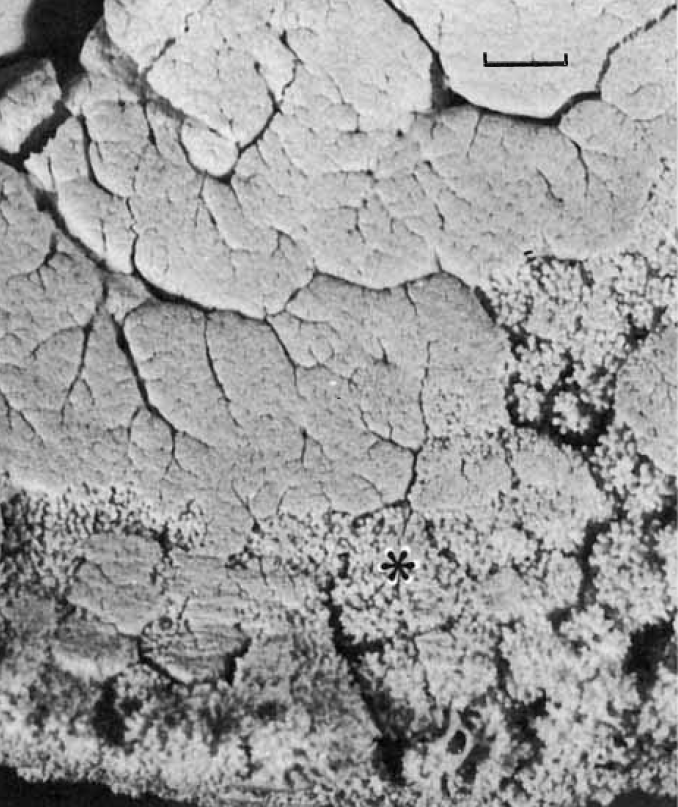
\includegraphics[width=0.35\textwidth,height=2in]{figures/images/upperlobe_haefeli1988.png}}                
  \subfloat[]{\label{fig:honey}\includegraphics[width=0.35\textwidth,height=2in]{figures/images/TB_to_aveolarduct_BerkeleyLungLabtour.png}}\\
  \subfloat[]{\label{fig:pores}\includegraphics[width=0.35\textwidth,height=2in]{figures/images/aveolarPores_BerkeleyLungLabLungtour.png}}
\subfloat[]{\label{fig:acini}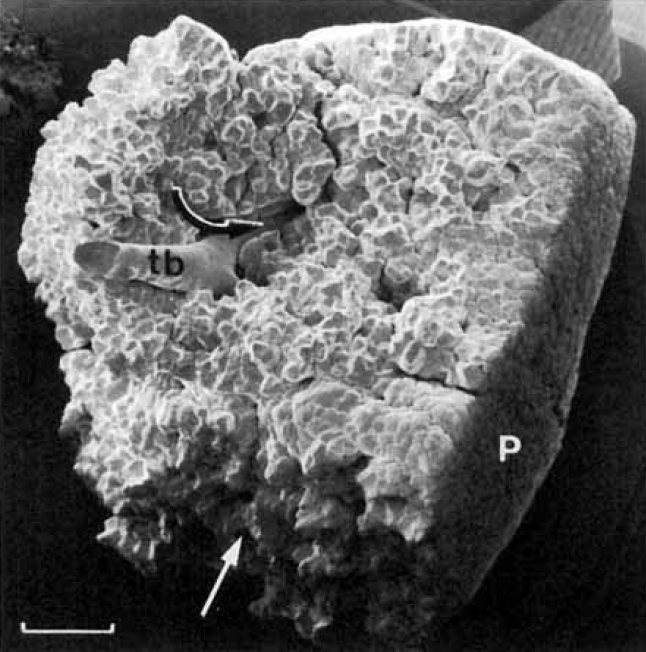
\includegraphics[width=0.35\textwidth,height=2in]{figures/images/acinus_HAEFELI-BLEUER1988.png}}
\caption{ (a) Portions of silicone rubber casts of upper lobes
of human lungs; asterisk marks incompletely filled regions. The outline of individual unfilled acinar units can also be seen. Scale marker, $5\;\mbox{mm}$. (b) Transition from terminal bronchiole to alveolar duct, from conducting airway to oxygen transfer area, diameter of terminal bronchiole is $0.5 \;\mbox{mm}$. (c) A few alveoli in an alveolar duct. The dark round openings are pores between alveoli. The alveolar wall is quite thin and contains a network of capillaries. The average diameter of one alveoli is $0.2\;\mbox{mm}$. (d) Scanning electron micrograph of complete acinus with transitional bronchiole
(tb) and surface abutting on pleura (P). Note the irregular surface where alveolar sacs of adjacent acini interdigitate (straight arrow). Scale marker, 1 mm. Images are reproduced from \cite{lunglab}.
 }
  \end{center}
   \label{fig:acinar_units}
\end{figure}
%
\begin{table}[h]
\begin{center}
\scalebox{0.76}{
\begin{tabular}{|l|c|c|c|c|c|c|}
\hline
Generation & Diameter & Length  & Flow rate 10L/min & Re & Flow rate 100L/min & Re \\
           & cm            & cm         &Velocity (m/s) &  & Velocity (m/s) & \\

\hline 
Trachea & 1.80 & 12.0 & 65.8 & 775 & 658 & 7750  \\
1 & 1.22 & 4.76 & 71.6 & 573 & 716 & 5730\\
5 & 0.35 & 1.07 & 53.6 & 123 & 536 & 1230\\
10 & 0.13 & 0.46 & 12.55 & 10.6 & 125 & 106\\
15 & 0.066 & 0.20 & 1.48 & 0.63 & 14.8 & 6.30\\
20 & 0.045 & 0.083 & 0.10 & 0.031 & 1.00 & 0.31\\

\hline
\end{tabular}
}
\end{center}
\caption{Shows dimensions, velocity and the corresponding Reynolds number for different sections of the airway tree during slow and rapid breathing. 
%Terminal bronchioles appear at around generation 15-16 which are then followed by respiratory bronchioles, the first generation to have alveoli. 
These values have been taken from \cite{pedley1970prediction}. }
\label{table:tree}
\end{table}
%
\begin{figure}[H]
  \centering
{\label{fig:mouse}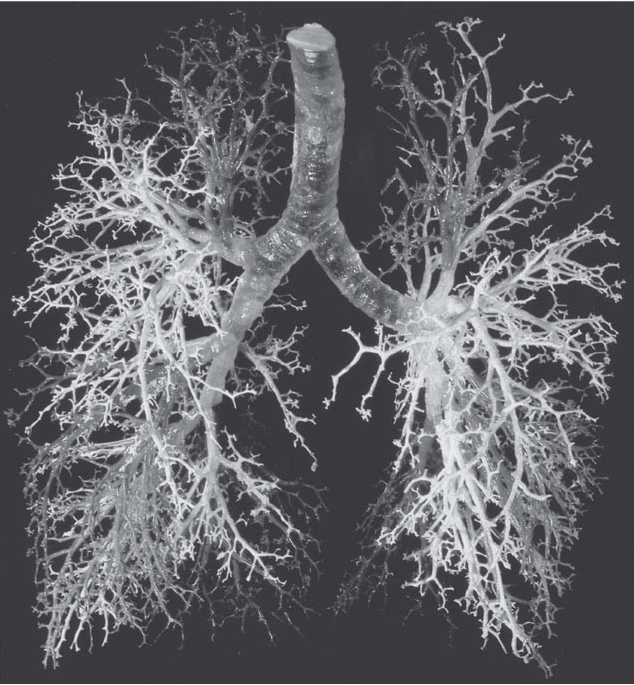
\includegraphics[width=0.5\textwidth]{figures/images/lung_west.pdf}}                
  \label{fig:acinar_units}
\caption{A rubber cast of the conducting of a human lung. The image is reproduced from \cite{west2008respiratory}.}
\label{fig:rubber_tree}
\end{figure}

%\subsubsection{Lung parenchyma} 
 Lung parenchyma refers to the portion of the lung made up of the small air chambers (alveoli) participating in gas exchange. The alveoli are made up of collagen, elastin fibers and membranous structures containing the capillary network, see Figure \ref{fig:pores}. Alveoli are arranged in sponge like structures and fill the entire volume of the lungs surrounding the conducting passages. Figure \ref{fig:sponge} shows a rubber cast of lung parenchyma, the dark lines outline the branching structure of the airways.
%The interior design of lung parenchyma is determined by the branching of the conducting airways. 
The right and left lung are partitioned into three and two lobes, respectively. Lung segments of conic shape are then the first subdivision of these lobes. These structures are bounded by connective tissue such that surgical separation is often possible. In the right lung, there are usually ten segments whereas only nine can be found in the left lung. Within the segments, the bronchi branch about six to twelve times. The terminal bronchioles which appear after roughly $15-16$ branching generations then finally feed into approximately $30,000$ so-called acini, see Figure \ref{fig:acini}. These acini represent the largest lung units of which all airways are alveolated and thus participate in gas exchange \cite{WeichertThesis}.
%
%
\begin{comment}
\subsection{Collateral ventilation.} 
Need to get a copy of the following paper:
``Collateral ventilation.
Menkes H, Traystman R, Terry P.
Abstract: Ventilation may bypass obstructed airways through collateral channels, including interalveolar pores of Kohn, bronchiole-alveolar communications of Lambert, and interbronchiolar pathways of Martin. Resistance through these channels, like resistance through small airways, increases with decreasing lung volume and with hypocapnia. But whereas the distention of collateral channels and small airways by a variety of factors is similar, the efficiency of ventilation through collateral channels is less than the efficiency through airways. Gas inspired through collateral channels is contaminated with alveolar gas from surrounding lung so that the dead space for collateral ventilation is increased. When one part of the lung ventilates out of phase with the surrounding lung, pulmonary interdependence promotes more homogeneous ventilation. In the presence of airways obstruction, interdependence may be a primary factor governing the rate of collateral ventilation. In man, collateral ventilation is unimportant in normal lungs. However, with disease, it may be critical in producing or compensating for abnormalities. For example, the long time constant for collateral ventilation in the middle lobe may be responsible for atelectasis, which results in the middle lobe syndrome. On the other hand, the short time constant for collateral ventilation in emphysema may be essential for the distribution of ventilation beyond obstructed airways.''

Also need to get:
``Collateral Ventilation and Gas Exchange during Airway Occlusion in the Normal Human Lung
Nicholas W. Morrell, C. Michael Roberts, Tony Biggs, and W. Anthony Seed''
\end{comment}
\begin{comment}

\begin{table}[H]
\begin{center}
\scalebox{0.7}{
\begin{tabular}{ l c c c c c}
\hline Parameter &  Description & Value& Reference  \\
\hline
$\rho^{s}$ & Density of alveolar tissue & ${1065\;\mbox{kg}}\,\mbox{m}^{-3}$ & \cite{hogg1969regional} \\
$\rho^{s}$ & Density of the alveolar wall & ${1000\;\mbox{kg}}\,\mbox{m}^{-3}$ & \cite{lande2006analysis}\\
$\rho^{f}$ & Density of of air at 27C$^\circ$ & ${1.18 \;\mbox{kg}}\,\mbox{m}^{-3}$ & Wiki \\
$\phi_{0}$ & Estimated reference porosity in the lung & $0.93$ & \cite{WeichertThesis} \\
$\mu^{f}$ & Viscosity for air at 27C$^\circ$ & $1.86 \times 10^{-5} \; \mbox{kg}\,\mbox{m}^{-1}\,\mbox{s}^{-1}$ & Wiki \\
$\bb{\kappa} $ &Permeability of the porous media (rough approximation) & $10^{-10}-10^{-12} \; \mbox{m}^{2}$ & \cite{owen2001mechanics},\cite{lande2006analysis}\\
$p $ &Mean airway pressure
 for high-frequency oscillation & $2000 \; \mbox{kg}\,\mbox{m}^{-1}\,\mbox{s}^{-2}$ & \cite{owen2001mechanics} \\
 $\hat{v} $ & Poisson ratio of porous lung at airway pressure $2000\,\mbox{Pas}$& $0.3$ & \cite{owen2001mechanics} \\
 
  $E $ & Young's modulus of lung tissue at airway pressure $2000\,\mbox{Pas}$& $8000$ $\mbox{kg}\,\mbox{m}^{-1}\,\mbox{s}^{-2}$  & \cite{owen2001mechanics} \\
  
  $\bb{u}^{s} $ & Tissue displacement near the diaphragm assuming sinusoidal motion & $0.05$ $\mbox{m}$  & \cite{gorman2002diaphragm} \\

  $\bb{a}^{s} $ & Tissue acceleration near the diaphragm assuming sinusoidal motion & $0.02$ $\mbox{m}\,\mbox{s}^{-2}$  & calculated \\

\hline
\end{tabular}
}
\end{center}
\caption{A collection of various parameters and typical values associated with lung parenchyma.} \label{tab:summary_equations}
\label{tab:parameters}
\end{table}
\end{comment}
%

%\section{Literature review}

%\input{/users/lorenzb/Dphil/poroelasticity_papers/coupling_paper/contents/literature}

\section{Computational lung models}
\label{section:review_models}
%
There exist a large number of computational ventilation and deformation models for the lung. Some models are designed to model particular phenomena whilst others are more general. They also range in spatial complexity from 0D compartment type models to 3D models which are able to incorporate `patient-specific' geometries extracted from CT images. In this review, we will focus on models that couple ventilation with tissue deformation and can be used as patient-specific models. A review of popular compartment based lung models can be found in \citet{bates2009lung}. 
%
One study that couples ventilation and tissue deformation using a one way coupling approach and then applies the model to a full 3D geometry is described in \citet{tawhai2010image}. Here a mechanics model for elastic deformation of compressible lung tissue is used to provide flow and pressure boundary conditions for an embedded airway model which makes the resultant ventilation distribution dependent on the tissue deformation due to gravity. In \citet{Swan2012}, air flow is simulated in patient specific conducting airways which are coupled to geometrically simplified terminal acinar units with varying volume dependent compliance. The fluid flow in the airways is approximated by Poiseuille flow with an added correction term for airway bifurcations. The end terminal acinar units are able to expand but are assumed to be independent of neighbouring acinar units. This does not allow for feedback from neighbouring acini that are infact tightly connected by a matrix of fibers, collagen and capillaries. 
%This model confirms experimental evidence that in the healthy lungs tissue compliance has a far greater effect than airway resistance on the spatial distribution of ventilation, and hence a realistic description of tissue deformation is essential in models of ventilation. 
Other sophisticated flow models of the whole airway tree, also exist \citep{yin2013multiscale,ismail2013coupled}. These models solve the full 3D Navier-Stokes equations in the upper airways, segmented from CT images, to capture high Reynolds number effects. The 3D fluid model is then coupled to a 0D laminar flow model of the lower airways. %None of these models incorporate the feedback of tissue deformation on ventilation and vice versa, and only loosely couple tissue deformation to ventilation.  


\section{Poroelastic models for lung parenchyma and other biological tissue}
%\label{section:poroelastic_review}
Some early work on a mechanical model of lung parenchyma as a poroelastic medium has already been proposed in \citet{kowalczyk1993mechanical}. This work developed a similar poroelastic model to the one we propose, however it has only been applied to a very simple 2D geometry. Also in \citet{owen2001mechanics} homogenisation theory has been used to derive macroscopic poroelastic equations for average air flows and tissue displacements in lung parenchyma during high frequency ventilation. The resulting model is a one dimensional system of equations that is used to investigate the effect of high-frequency ventilation on strain in the parenchymal tissue. The use of a poroelastic model has also been applied to modelling other biological tissues. For example modelling protein based hydrogels embedded with cells \citep{galie2011linear}, perfusion of blood flow in the beating myocardium \citep{chapelle2010poroelastic,cookson2011novel}, the modelling of brain oedema (swelling) \citep{li2010three} and hydrocephalus \citep{wirth2006axisymmetric}. Another application is the modelling of interstitial fluid and tissue in articular cartilage and intervertebral discs \citep{mow1980biphasic,holmes1990nonlinear,galbusera2011comparison}.




\begin{comment}
%One study presented a framework for coupling models of ventilation and tissue deformation \cite{tawhai2006imaging}. First, changes in geometry of the lung mesh are determined and used to compute flow through an airway model. Pressures are then interpolated throughout the lung mesh to provide hydrostatic pressures that act as input loads for the mechanics model, which is then solved to predict shape change. These deformations are used to compute local volume changes which feed back as inputs to the flow-pressure problem and the system is solved iteratively. In these models tissue deformation is not directly dependent on ventilation, however an integrated model of ventilation and tissue mechanics model will be particularly important for understanding respiratory diseases since nearly all pulmonary diseases lead to some abnormality of lung tissue mechanics  \cite{suki2011lung}. For example, Chronic Obstructive Pulmonary Disease (COPD) encompasses emphysema (destruction of alveolar tissue) and chronic 
bronchitis which can cause severe bronchoconstriction and atelectasis (air trapping), both of which can significantly alter tissue properties. If the tissue mechanics are affected so too will the ventilation and vice versa emphasising the importance of a model that fully couples the tissue mechanics and ventilation in the lung. 

%There has been one study that presents a framework for coupling models of ventilation and tissue deformation \cite{tawhai2006imaging}. First, changes in geometry of the lung mesh are determined and used to compute flow through an airway model. Pressures are then interpolated throughout the lung mesh to provide hydrostatic pressures that act as input loads for the mechanics model, which is then solved to predict shape change. These deformations are used to compute local volume changes which feed back as inputs to the flow-pressure problem and the system is solved iteratively.

 %Although it is assumed that lung tissue is a continuum with uniform material properties, simulations of tissue deformation in a realistic geometry can give rise to a considerable degree of heterogeneity. 
%Including this model of tissue deformation in a ventilation model clearly predicts more physiologically consistent ventilation distributions than simply assuming that tissue compliance is constant or proportional to lung height. Therefore we conclude  that it is an essential feature in functional computational models of ventilation which aim to describe ventilation and perfusion matching or changes in ventilation distribution with disease.
%Another model that incorporates subject-specific anatomical geometry and approximates the airways by Poiseuille flow with an added correction term for airway bifurcations is presented in \cite{HedgesThesis}, here the aim is to predict forced expiration (FEV1) values. 

\end{comment}



 
%The model confirms experimental evidence that in the healthy lungs tissue
%compliance has a far greater effect than airway resistance on the spatial distribution of ventilation, and hence a realistic description of tissue deformation is essential in models of ventilation.
%Although it is assumed here that lung tissue is a continuum with uniform material properties, simulations of tissue deformation in a curvilinear geometry can give rise to a considerable degree of heterogeneity. Including this model of tissue deformation in a ventilation model clearly predicts more physiologically consistent ventilation distributions than simply assuming that tissue compliance is constant or proportional to lung height. Therefore we conclude  that it is an essential feature in functional computational models of ventilation which aim to describe ventilation and perfusion matching or changes in ventilation distribution with disease.''  \cite{SwanThesis}

 %However in this model, tissue deformation is not directly dependent on ventilation.


%Due to the often high Reynolds numbers in the upper airways, 3D fluid flow models have been used to model this sections of the airway tree. Clearly approximating the entire airway tree using 3D fluid flow remains intractable due to constraints on imaging resolution and computational power. Therefore smaller airways still need to be generated using a volume-filling branching algorithm \cite{tawhai2004ct} and then approximated by simpler 1D flow equations. The coupling of a 3D flow model to a 1D flow model for a complete airway tree has already been done in \cite{lin2009multiscale} and is achieved through mass conservation. i.e. the flow rates at the exit faces of the 3-D airway model can be determined by summing the flow rates at the terminal bronchioles using the connectivity information between the 3-D airway exit faces and the associated downstream 1-D airway branches. However this summing of flow rates is unable to account for any changes in resistances in the airway tree which might have been introduced 
%due to disease, for example bronchoconstriction or the collapsing of airways which is common in many types of COPD. There has also been sophisticated work on 3D to 1D fluid flow coupling for modelling blood flow with compliant vessels in the cardiovascular system \cite{formaggia2001coupling} and cerebral vasculature \cite{passerini20093d}.



%\input{/users/lorenzb/Dphil/poroelasticity_papers/large_deformation/contents/review}
\section{Finite element methods for poroelasticity}
The method that we use for spatially discretising our equations in this work is the finite element method (FEM) for obtaining approximations to the solution of partial differential equations.

After many decades of research there remain numerous challenges associated with the numerical solution of the poroelastic equations. When using the finite element method the main challenge is to ensure stability and convergence of the method and prevent numerical instabilities that often manifest themselves in the form of spurious oscillations in the pressure. It has been suggested that this problem is caused by the saddle point structure in the coupled equations resulting in a violation of the famous Ladyzhenskaya-Babuska-Brezzi (LBB) condition \citep{haga2012causes}, highlighting the need for a stable combination of mixed finite elements. Another numerical challenge in practical 3D applications is the algebraic system arising from the finite element discretisation. This can lead to a very large matrix system that has many unknowns and is severely ill-conditioned, making it difficult to solve using standard iterative solvers. Therefore low-order finite element methods that allow for efficient preconditioning are preferred \citep{white2011block,ferronato2010fully}.

\subsection{Linear three-field discretisations}
The poroelastic equations are often solved in a reduced displacement and pressure formulation, from which the fluid flux can then be recovered \citep{murad1994stability,white2008stabilized}. \citet{murad1994stability} have analysed the stability and convergence of this reduced displacement pressure $(\boldsymbol{u}/ p)$ formulation and were able to show error bounds for inf-sup stable combinations of finite element spaces (e.g. Taylor-Hood elements). In this paper we will keep the fluid flux variable resulting in a three-field, displacement, fluid flux, and pressure formulation. Keeping the fluid flux as a primary variable has the following advantages:
\begin{enumerate}[label=\roman*]
 \item It avoids the calculation of the fluid flux in post-processing. 
\item Physically meaningful boundary conditions can be applied at the interface when modelling the interaction between a fluid and a poroelastic structure \citep{badia2009coupling}.
 \item It allows for greater accuracy in the fluid velocity field. This can be of interest whenever a consolidation model is coupled with an advection diffusion equation, e.g. to account for thermal effects, contaminant transport or the transport of nutrients or drugs within a porous tissue \citep{khaled2003role}.
 \item It allows for an easy extension of the fluid model from a Darcy to a Brinkman flow model, for which there are numerous applications in modelling biological tissues \citep{khaled2003role}.
 \item It reduces the order of the spatial derivative of the pressure, allowing for a discontinuous pressure approximation without any additional penalty terms.
\end{enumerate}

\citet{phillips2007coupling,phillips2007couplingtwo}, have proven error estimates when solving the three-field formulation problem using continuous piecewise linear approximations for displacements and mixed low-order Raviart Thomas elements for the fluid flux and pressure variables. However this method was found to be susceptible to spurious pressure oscillations \citep[see,][]{phillips2009overcoming}. To overcome these pressure oscillations, \citet{li2012discontinuous} analysed a discontinuous three-field method, and \citet{yi2013coupling} analysed a nonconforming three-field method.
%In \citet{li2012discontinuous}, a discontinuous method and in \citet{yi2013coupling} a nonconforming three-field method is analysed. These papers were motivated by the need for a method that is able to overcome pressure oscillations \citep[see,][]{phillips2009overcoming} experienced by the method in \citet{phillips2007coupling,phillips2007couplingtwo}. 
In addition to these monolithic approaches there has been considerable work on operating splitting (iterative) approaches for solving the poroelastic equations \citep{wheeler2007iteratively,feng2010fully,kim2011stability}. Although these methods are often able to take advantage of existing elasticity and fluid finite element software, and result in solving a smaller system of equations, these schemes are often only conditionally stable. To ensure that the method is unconditionally stable, monolithic approaches are often preferred. The method proposed in this work is monolithic, and will therefore retain the advantage of being unconditionally stable .

%\subsection{Stability of Darcy-Stokes formulation}
%Numerous stabilization techniques for finite element methods have already been proposed in order to satisfy the LBB condition, most extensively for the model equations of Stokes and Darcy flow, which despite their simplicity retain all the difficulties of a saddle point problem. This will be discussed again in more detail in section \ref{sec:mixed}. Another good introduction on stabilization techniques for the Stokes problem can be found in chapter 5 of \citet{elman2005finite}. For a comparison of low-order stabilization techniques for the Darcy problem we refer to \citet{bochev2006computational}. Most stabilized methods lead to a modified variational formulation in which an additional term is added to the mass balance equation, modifying the incompressibility constraint
%in such a way that stability of the mixed formulation is increased,
%while still maintaining optimal convergence of the method. These stabilization techniques are of great interest to us since solving the three-field poroelasticity problem is essentially equivalent to coupling the Stokes equations (elasticity of the porous mixture) with the Darcy equations (fluid flow through pores), with a modified incompressibility constraint that combines the divergence of the displacement velocity and the fluid flux. 







%After many decades of research there remain numerous challenges associated with the numerical solution of the poroelastic equations valid in small and large deformations. When using the finite element method the main challenge is to ensure stability and convergence of the method and prevent numerical instabilities that often manifest themselves in the form of oscillations in the pressure. It has been suggested that this problem is caused by the saddle point structure in the coupled equations resulting in a violation of the famous Ladyzhenskaya-Babuska-Brezzi (LBB) condition \citep{haga2012causes}, highlighting the need for a stable combination of mixed finite elements. Another numerical challenge in practical 3D applications is the algebraic system arising from the finite element discretization. These theoretical stability issues have already been studied for some linear (small deformation) poroelasticity formulations \citep{murad1994stability,haga2012causes} and numerous remedies have been proposed \citep{phillips2007coupling,phillips2007couplingtwo,li2012discontinuous,yi2013coupling,berger2014stabilized}.
\subsection{Methods valid in large deformations}


We will now give a brief overview of different approaches for solving the poroelastic equations valid in large deformations. There has been some work on operating splitting (iterative) approaches where the poroelastic equations are separated into a fluid problem and deformation problem \citep{chapelle2010poroelastic}. Again, this approach is only conditionally stable. Some notable quasi-static incompressible large deformation monolithic approaches include a mixed-penalty formulation, and a mixed solid velocity-pressure formulation, both outlined in \citep{almeida1998finite}, the solid velocity-pressure formulation is similar to the commonly used reduced $(\boldsymbol{u}/p)$ formulation \citep{ateshian2010finite}. These two-field $(\boldsymbol{u}/p)$ formulations require a stable mixed element pair such as the popular Taylor-Hood element to satisfy the LBB inf-sup stability requirement. To reduce the number of unknowns, and allow for an equal-order, piecewise linear approximation, a stabilized reduced $(\boldsymbol{u}/ p)$ formulation has been proposed in \citep{white2008stabilized}. This method introduces a stabilization term to the mass conservation equation to overcome the spurious pressure oscillations. The key difficulty, however, that this stabilized element cannot escape is that jumps in material coefficients may introduce large solution gradients across the
interface, requiring severe mesh refinement. This is because a continuous pressure element is used, which is unable to reliably capture jumps in the pressure solution \citep{white2008stabilized}. In \citep{levenston1998variationally} a three-field (displacement, fluid flux, pressure) formulation has been outlined, however this method uses a low-order mixed finite element approximation without any stabilization and therefore is not inf-sup stable.





 


%\input{/users/lorenzb/Dphil/poroelasticity_papers/ima_submission/introduction_jcam}

\chapter{Poroelasticity theory}
\input{/users/lorenzb/Dphil/poroelasticity_papers/large_deformation/contents/intro_theory}
\section{Kinematics}
\input{/users/lorenzb/Dphil/poroelasticity_papers/large_deformation/contents/continuum_mechanics_theory}

%\section{Mixture theory}
\input{/users/lorenzb/Dphil/poroelasticity_papers/large_deformation/contents/mixture_theory}


\section{Linear poroelasticity}
\label{sec:themodel}
To allow us to perform rigorous analysis of the proposed finite element scheme presented in Chapter \ref{chap:linear_poro}, we will now assume small deformations to yield a linear model of poroelasticity. This model is often referred to as the `Biot model' in the geomechanics community and contains some additional terms. We will introduce the full Biot model here for use with a 2D cantilever bracket problem later tested in section \ref{section:overcoming}, and to highlight that any subsequent theory developed in later chapters can be extended to the full Biot model. The governing equations of the Biot model, with displacement $\dispcont$, fluid flux $\fluxcont$, and pressure $\pcont$ as primary variables are summarized below:  
\begin{subequations}
\begin{align}
\label{eqn:strong_mixture_momentum}
- \nabla \cdot \mathbf{\sigma}  =\mathbf{f} \;\;\; \mbox{in}\; \Omega \times (0,T),\\
{\perm^{-1}\mathbf{z}} + \nabla p =  \mathbf{b} \;\;\; \mbox{in}\; \Omega\times (0,T), \\
\nabla \cdot \mathbf{z} + \pderiv{}{t}(\alpha\nabla \cdot \mathbf{u} + c_{0} p )  = g   \;\;\; \mbox{in}\; \Omega \times (0,T),
\\
\mathbf{u} =\mathbf{u}_{D}   \;\;\; \mbox{on}\; \Gamma_{D} \times (0,T),
\\
\mathbf{\sigma}\mathbf{n} = \mathbf{t}_{N}   \;\;\; \mbox{on}\; \Gamma_{N} \times (0,T),
\\
p = p_{D}   \;\;\; \mbox{on}\; \Gamma_{P} \times (0,T),
\\
\mathbf{z}\cdot \mathbf{n} = {q_{D}}   \;\;\; \mbox{on}\; \Gamma_{F} \times (0,T),
\\
\mathbf{u}(0,\cdot) = \mathbf{u}^{0},  \;\;\; p(0) = p^{0}, \;\;\; \mbox{in}\; \Omega.
\end{align}
\label{eqn:strong_cont_system_biot}
\end{subequations}
Here $\mathbf{\sigma}$ is the total stress tensor given by $\mathbf{\sigma}=\lambda \mbox{tr}(\mathbf{\epsilon}(\dispcont))\identity + 2\mu_{s}\mathbf{\epsilon}(\dispcont)-\alpha p\mathbf{I}$, with the linear strain tensor defined as $\mathbf{\epsilon}(\dispcont)=\frac{1}{2}\left(\nabla \dispcont + \left( \nabla \dispcont \right)^{T} \right)$, $g$ is the fluid source term, $\mathbf{f}$ is the body force on the mixture, and $\mathbf{b}$ is the body force on the fluid.  Here $\Omega$ is a bounded domain in $\mathbb{R}^{2}$ or $\mathbb{R}^{3}$, and for the purpose of defining boundary conditions, $\partial\Omega=\Gamma_D+\Gamma_N$ for displacement and stress boundary conditions and  $\partial\Omega=\Gamma_P+\Gamma_F$ for pressure and flux boundary conditions, with outward pointing unit normal $\mathbf{n}$. The parameters along with a description are given in Table \ref{tab:parameters}.
\begin{table}[H]
\begin{center}
\scalebox{0.9}{
\begin{tabular}{ l c c }
\hline
\bf Parameter &    \\
\hline
Lam\'{e}'s first parameter &  $\lambda$,  \\
Lam\'{e}'s second parameter (shear modulus)  &  $\mu_{s}$,  \\
Dynamic permeability tensor &  $\perm$,  \\
%Solid skeleton density &  $\rho_s$  \\
%Fluid density &  $\rho_f$  \\
Biot-Willis constant &  $\alpha$,  \\
Constrained specific storage coefficient &  $c_{0}$.
\end{tabular}
}
\end{center}
\caption{Poroelasticity parameters.} 
\label{tab:parameters}
\end{table}
\noindent A derivation and more detailed explanation of these equations can be found in \citet{phillips2007coupling} and \citet{showalter2000diffusion}. In this work we will mainly consider a simplification of the full Biot model (\ref{eqn:strong_cont_system_biot}), by setting $\alpha=1$ and $c_{0}=0$. This yields a fully incompressible poroelastic model that retains all the numerical difficulties associated with approximating the original system of equations (\ref{eqn:strong_cont_system_biot}), see Remark \ref{remark:extension}. The linear fully saturated and incompressible poroelastic model is given by: 
\begin{subequations}
\begin{align}
\label{eqn:strong_mixture_momentum_simple}
-(\lambda+\mu_{s}) \nabla (\nabla\cdot\mathbf{u})-\mu_{s} \nabla^{2} \mathbf{u} + \nabla p = \mathbf{f} \;\;\; \mbox{in}\; \Omega\times (0,T),\\
{\perm^{-1}\mathbf{z}} + \nabla p =  \mathbf{b} \;\;\; \mbox{in}\; \Omega\times (0,T),\\
\nabla \cdot (\mathbf{u}_{t} + \mathbf{z} )  = g   \;\;\; \mbox{in}\; \Omega\times (0,T),
\\
\mathbf{u} =\mathbf{u}_{D}   \;\;\; \mbox{on}\; \Gamma_{D}\times (0,T),
\\
\mathbf{\sigma}\mathbf{n} = \mathbf{t}_{N}   \;\;\; \mbox{on}\; \Gamma_{N}\times (0,T),
\\
p = p_{D}   \;\;\; \mbox{on}\; \Gamma_{P}\times (0,T),
\\
\mathbf{z} \cdot \mathbf{n} = {q_{D}}   \;\;\; \mbox{on}\; \Gamma_{F}\times (0,T),
\\
\mathbf{u}(0,\cdot) = \mathbf{u}^{0}  \;\;\;  \mbox{in}\;\Omega.
\end{align}
\label{eqn:linear_simple_system}
\end{subequations}

\noindent This model is the small deformation version of the simplified and reformulated large deformation poroelasticity model (\ref{eqn:simple_mixture_model}), and will be the small deformation model considered from here onwards.


\begin{remark}
The extension of the theoretical results presented in Chapter \ref{chap:linear_poro} from (\ref{eqn:linear_simple_system}) to the full Biot equations (\ref{eqn:strong_cont_system_biot}), with $\alpha \in \mathbb{R}_{> 0} \text{ and } c_{0}\in \mathbb{R}_{> 0}$ is straightforward. In the analysis in Chapter \ref{chap:linear_poro}, the constant $\alpha$ would just get absorbed by a general constant $C$. When $c_{0}>0$, an additional pressure term is introduced into the mass conservation equation. Since this term is coercive, it only improves the stability of the system.
\label{remark:extension}
\end{remark}








%% FEM intro
\chapter{Finite element method}

\section{Introduction}
%Miguel
A large proportion of the mathematical models in science and engineering take the
form of differential equations. Only in the simplest cases, or under strong assumptions,
is it possible to find exact analytical solutions to the equations in the model.
%Often, one has to rely on numerical techniques for finding approximate solutions
%for particular parameter sets using computers. 
%The finite element method is a general
%technique for the numerical solution of differential equations. 
%
%The method was introduced by engineers in the late 1950's and early 1960's for the numerical
%solution of PDEs in structural engineering. When the mathematical study
%of the finite element method started in the mid 1960's it soon became clear that in
%fact the method is a general technique for numerical solution of partial differential
%equations with roots in the variational methods in mathematics introduced at the
%beginning of the 20th century.
%
%
%
%
%Lyia
Numerical methods are an established means of solving differential equations that are
of practical interest in a variety of applied problems. Finite difference, finite volume
and finite element methods are the most widely used types of such methods. Their
basic idea is replacing the infinite-dimensional problem by a finite-dimensional
approximation, which is, generally speaking, easier to compute.
%
%The main idea of finite difference methods is to approximate the derivatives appearing
%n the equations with finite differences at a set of discrete points in the domain
%of interest. Their advantages include relative simplicity of derivation and implementation.
%However, finite difference methods are best suited for simple domain shapes
%and regular meshes, while using them for problems on complex geometries requires
%non-standard treatment even for standard differential equations. For an introduction
%to finite differences in partial differential equations we refer to [90, 116, 114].
%Finite volume methods [87, 121] rely on the application of the divergence theorem
%within small subdomains of the original domain – finite volumes – and approximating
%fluxes through volume boundaries. These methods are traditionally used in the
%field of computational fluid dynamics due to their conservative properties, although
%9
%formulating problems on complex geometries is again far from trivial.
Finite element methods are based on weakening the restrictions on the solution
space in the continuous setting, and searching for the approximate solution in the
subspace which spans basis functions supported on small regions inside the domain.
These methods are well-suited to solving problems on complex domains, and are
therefore widely used in practical applications.
In this work we consider only finite element methods (FEMs) for solving partial
differential equations.
This chapter comprises an overview of several theoretical and practical aspects of classical FEMs. The theory and notation presented here are essential in developing
the techniques that form the core of this thesis. Most of the work presented in this chapter is based on work already presented in \citet{arthursthesis,asnerthesis,bernabeusthesis,brenner2008mathematical,f1991mixed}.


%
%Chris
%The method that we use for spatially discretising our equations in this work is the finite
%element method (FEM) for obtaining approximations to the solution of partial differential
%equations. It was introduced in its present form in 1942 by Richard L. Courant as an
%appendix to his paper on variational methods [75], although it does not then appear in
%the literature again for another sixteen years [76]. It was further developed by engineers
%during the late 1950s and early 1960s as a method of solving equations in structural engineering
%[77], and has since developed into a general tool for the numerical approximation
%of solutions to PDEs.
\section{Norms and spaces}
Let $\Omega$ be a bounded domain in $\mathbb{R}^{2}$ or $\mathbb{R}^{3}$, and $\partial\Omega$ be the associated boundary. The space of square integrable functions is then given by
\begin{equation*}
L^{2}(\Omega)  = \left\lbrace  u : \int_{\Omega} |u(x)|^{2} \mbox{d}x < \infty \right\rbrace,
\end{equation*}
with norm
\begin{equation*}
\ltwonorm{u}  = \left\lbrace \int_{\Omega} |u(x)|^{2} \mbox{d}x  \right\rbrace^{1/2}.
\end{equation*}
This space is equipped with the inner product
\begin{equation*}
(u,v)  :=  \int_{\Omega} u(x)v(x) \mbox{d}x,
\end{equation*}
such that $\ltwonorm{u}=(u,v)^{1/2}$. Throughout this thesis we shall frequently refer to the Sobolev spaces
$H^{1}(\Omega)$ and $H^{2}(\Omega)$. The definitions of these are as follows:
%
\begin{equation*}
H^{1}(\Omega)  = \left\lbrace  u  \in L^{2}(\Omega): \frac{\partial u }{\partial x_{j}} \in L_{2}(\Omega) , \; j=1,\ldots ,n, \right\rbrace,
\end{equation*}
\begin{equation*}
H^{2}(\Omega)  = \left\lbrace  u  \in L^{2}(\Omega): \frac{\partial u }{\partial x_{j}} \in L_{2}(\Omega) , \; j=1,\ldots ,n, \;  \frac{\partial^{2} u }{\partial x_{i} \partial x_{j}} \in L_{2}(\Omega), \; i,j=1,\ldots ,n \right\rbrace.
\end{equation*}
The corresponding norms are defined as
\begin{equation*}
\honenorm{u}  = \left\lbrace \ltwonorm{u}^{2} + \sum_{j=1}^{n} \ltwonorm{\frac{\partial u }{\partial x_{j}}}   \right\rbrace^{1/2},
\end{equation*}
\begin{equation*}
\htwonorm{u}  = \left\lbrace \ltwonorm{u}^{2} + \sum_{j=1}^{n} \ltwonorm{\frac{\partial u }{\partial x_{j}}}  + \sum_{i,j=1}^{n} \ltwonorm{\frac{\partial^{2} u }{\partial x_{i} \partial x_{j}}}  \right\rbrace^{1/2}.
\end{equation*}
We also define the divergence space 
\begin{equation*}
H_{div}(\Omega)=\left\lbrace \boldsymbol{v}\in L^{2}(\Omega): \nabla \cdot \boldsymbol{v} \in L^{2}(\Omega) \right\rbrace.
\end{equation*}
The set of functions of $L^{2}(\partial \Omega)$ which are traces of functions of $H^{1}(\Omega)$ onto the boundary, constitutes a subspace of $L^{2}(\partial \Omega)$ denoted by $H^{1/2}(\partial \Omega)$. We will also briefly use linear and bounded functionals (dual spaces) of $H^{1},H^{1/2}$ and $H_{div}$, which will be denoted by $H^{-1},H^{-1/2}$ and $H_{div}^{-1}$, respectively. 

We define the following norms for continuous in time functions $u$ such that the norm $L^2(0,T; X)$ satisfies
\begin{equation*}
 || u ||_{L^2( X) }= \left( \int_0^T || u (s,\cdot) ||^2_X ~ds \right)^{1/2},
\end{equation*}
and the norm $L^{\infty}(0,T; X)$ satisfies
\begin{equation*}
 || u ||_{L^{\infty}(X) }= \sup\left\lbrace ||{u (s,\cdot)}||_{X} : s \in [0,T] \right\rbrace,
\end{equation*}
where $X$ is any given function space over $\Omega$. We partition $[0,T]$ into $N$ evenly spaced non-overlapping regions $(t_{n-1}, t_n]$, $n=1,2,\dots, N$. For any sufficiently smooth function $u(t,x)$ we define $u^n(x) = u(t_n,x)$. Let the discrete approximation for all time to be the piecewise constant in time functions $v(t,{\bf x})  := v^n({\bf x})$ for $t \in (t_{n-1}, t_n]$. For such piecewise constant in time functions, $v$, we define the norms
\begin{equation*}
 || v ||_{L^2( X) }= \left( \sum_{n=1}^N \Delta t   || v^n||^2_X \right)^{1/2},
\end{equation*}
and
\begin{equation*}
 || v ||_{L^{\infty}( X) }= \max\left\lbrace ||{v^n}||_{X}, n=1,2,...,N \right\rbrace.
\end{equation*}




\begin{comment}

Finally we define the following continuous time-dependent norms 
\begin{equation*}
   \doublenorm{v}_{L^{2}(L^{2})} = \left( \int_{0}^{T} \ltwonorm{v(\cdot,t_{n})}^{2} dt \right)^{1/2}            ,                                                                                                                                                                                                                                                                                                                                                                                                                                                                                                                                                                                                                                                                                                                                                                                                                                                                                                                                                                                                                                                                                         \end{equation*}
   \begin{equation*}
   \doublenorm{v}_{L^{\infty}(L^{2})} =  \sup\left\lbrace \ltwonorm{v(\cdot,t_{n})} : t_{n} \in [0,T] \right\rbrace,                                                                                                                                                                                                                                                                                                                                                                                                                                                                                                                                                                                                                                                                                                                                                                                                                                                                                                                                                                                                                                                                                                    \end{equation*}
and their discrete in time counterparts
\begin{equation*}
  \doublenorm{v}_{l^{2}(L^{2})} = \left( \sum_{n=0}^{N} \Delta t_{n} \ltwonorm{v(\cdot,t_{n})}^{2} \right)^{1/2}            ,                                                                                                                                                                                                                                                                                                                                                                                                                                                                                                                                                                                                                                                                                                                                                                                                                                                                                                                                                                                                                                                                                         \end{equation*}
   \begin{equation*}
  \doublenorm{v}_{l^{\infty}(L^{2})} =  \max\left\lbrace \ltwonorm{v(\cdot,t_{n})} : t_{n} \in [0,t_{1},t_{2},...,T] \right\rbrace.                                                                                                                                                                                                                                                                                                                                                                                                                                                                                                                                                                                                                                                                                                                                                                                                                                                                                                                                                                                                                                                                                           \end{equation*} Definitions for slightly different combinations of temporal and spatial norms such as $\doublenorm{v}_{H^{1}(L^{2})}$ are straightforward adaptations of the above. Additional shorthand notation will be introduced throughout the thesis as is needed.

\end{comment}




%Let $L^{2}(\Omega)  := \left\lbrace  u : \int_{\Omega} u^{2} < \infty %\right\rbrace$ be the usual space of square integrable functions with inner %product $(v,w)=  \int_{\Omega} v(x)w(x) \mbox{d}x $ and norm $\ltwonorm{v}= %(v,v)^{1/2}$. We further define $L_{0}^{2}=\lbrace \pconttest \in L^{2}(\Omega): %\int_{\Omega} \pconttest = 0  \rbrace$.  
%
%We also introduce the space of functions with derivatives $\partial^{{\alpha}}v \in L^{2}(\Omega)$ for $|{\alpha}| \leq m$, where $ {\alpha}=\left\lbrace \alpha_{1}, \alpha_{2} \right\rbrace$, $|{\alpha}|= \alpha_{1}+\alpha_{2}$, $\alpha_{i}$ non-negative integers, equipped with the inner product $(v,w)_{m}=  \int_{\Omega} \partial^{\alpha} v(x) \partial^{\alpha}w(x) \mbox{d}x $ and norm $\hmnorm{v}= (v,v)_{m}^{1/2}$. 
%
%
%
\section{Model problem}
It is instructive to begin at a simple level and proceed by incrementally adding to the
complexity of the equations we are discretising when explaining the use of the FEM, so
we begin by considering the classical heat equation: given $T>0$, for $t \in[0,T]$ find $u(t,x)$ such that
\begin{subequations}
\begin{align}
\label{eqn:heat_strong}
\frac{\partial u}{\partial t} - \nabla \cdot \nabla u = 0\;\;\; \mbox{in} \; \Omega_{t},\\
\boldsymbol{n} \cdot \nabla u = {g}_{N}   \;\;\; \mbox{on}\; \Gamma_{N},
\\
\label{eqn:heat_dirichlet}
 u = {g}_{D}   \;\;\; \mbox{on}\; \Gamma_{D},
\\
 u(0,x) = u^{0}(x)   \;\;\; \mbox{in}\; \Omega.
\end{align}
\label{eqn:laplace}
\end{subequations}
Here $\Omega$ is a bounded domain in $\mathbb{R}^{2}$ or $\mathbb{R}^{3}$, with boundary $\partial\Omega = \Gamma_{N}  \cup \Gamma_{D} $, that has an outward pointing unit normal $\boldsymbol{n}$. The initial condition is given by $u^{0}(x)$. In the case where ${g}_{N}= 0$, system (\ref{eqn:laplace}) can describe the evolution of heat in an
object with geometry described by $\Omega$, where we have perfect thermal insulation on $\Gamma_{N}$ and fixed temperature distributions given by the function ${g}_{D}$ defined on the boundary due to some part of the environment with fixed temperature contacting the object along $\Gamma_{D}$.

\subsection{Weak formulation}

The strong form of (\ref{eqn:laplace}) requires $u$ to be at least twice differentiable. To weaken the regularity restrictions we multiply equation (\ref{eqn:heat_strong}) by an arbitrary function $v$, called a test function, and integrate over $\Omega$: 
\begin{equation*}
\left( \frac{\partial u}{\partial t},v \right)  -\left(\nabla \cdot \nabla u,v \right) = 0.
\end{equation*}
Applying the divergence theorem, this equation can be rewritten:
\begin{multline*}
\left( \frac{\partial u}{\partial t},v \right)  -\left(\nabla u \cdot \normal ,v \right)_{\partial \Omega}+ \left(\nabla u,\nabla v \right)\\= \left( \frac{\partial u}{\partial t},v \right)  -\left(\nabla u \cdot \normal ,v \right)_{\Gamma D}-\left(g_{N} ,v \right)_{\Gamma N}+ \left(\nabla u,\nabla v \right)=0.
\end{multline*}
Here $\left(\cdot ,\cdot\right)_{\Gamma_{N}}$ and $\left(\cdot ,\cdot\right)_{\Gamma_{D}}$ denote the inner product taken over $\Gamma_{N}$ and $\Gamma_{D}$, respectively. Taking note of the Dirichlet condition (\ref{eqn:heat_dirichlet}), and letting $v = 0$ on $\Gamma_{D}$, we arrive at the following equation:
\begin{equation*}
\left( \frac{\partial u}{\partial t},v \right) + \left(\nabla u,\nabla v \right)=\left(g_{N} ,v \right)_{\Gamma N}.
\end{equation*}
Note that in this equation the second derivatives of $u$ need not exist. With that in mind, both the solution and the test functions can come from the space $H^1(\Omega)$, as long as they satisfy the appropriate Dirichlet boundary conditions. For convenience we will use the notation $X_{D}=\left\lbrace v \in H^{1}(\Omega) | v = u_{D} \;\mbox{on} \; \Gamma_{D} \right\rbrace$ and $X_{0}=\left\lbrace v \in H^{1}(\Omega) | v = 0 \;\mbox{on} \; \Gamma_{D} \right\rbrace$. The weak formulation of (\ref{eqn:heat_strong}) is as follows: Find $u\in X_{D}$ such that
\begin{equation}
\left( \frac{\partial u}{\partial t},v \right) + \left(\nabla u,\nabla v \right)=\left(g_{N} ,v \right)_{\Gamma N}\;\;\forall v \in X_{0}.
\label{eqn:heat_weak}
\end{equation}

\subsection{Time discretisation}

We also need to choose a method of treating the time derivative. In this work, we do so using Euler difference quotients, and so we make the approximation $u_{t}(t+\Delta t,x) \approx \frac{u(t+\Delta t,x) - u(t,x)}{\Delta t}$ for some constant time step $\Delta t$. We write $u(x)^{n}$ for the the temporally-semidiscrete approximation to $u(n\Delta t,x)$, and our numerical scheme will yield approximations at times $t=0,\Delta t,2\Delta t,...,T$. Inserting this difference quotient and assuming that $\Delta T$ divides $T$, equation (\ref{eqn:heat_weak}) becomes: for $n=1,2,...,\frac{T}{\Delta t}$, find $u^{n}\in X_{D}$ such that
\begin{equation}
\left( u^{n},v \right) + \Delta t \left(\nabla u^{n},\nabla v \right)=\left(g_{N} ,v \right)_{\Gamma N}+\left( u^{n-1},v \right) \;\;\forall v \in X_{0}.
\label{eqn:heat_weak}
\end{equation}
%
\subsection{Finite element discretisation}
In order to solve this problem numerically, we must make it finite dimensional by discretising it suitably. The finite element approximation space is constructed as follows: first, the problem domain is partitioned into small element domains, and second, the element is defined by prescribing for each element domain a set of nodes and nodal values, and defining  suitable basis functions on these, for example, as piecewise-linear basis functions. 

Element domains are normally shaped as triangles or squares in $\mathbb{R}^{2}$, tetrahedra or hexahedra in $\mathbb{R}^{3}$. All the nodes, edges and faces of element domains constitute
the problem mesh. Defining local basis functions completes the finite element space. For a rigorous definition of finite elements, and a description of different types of elements we refer to \citet{brenner2008mathematical}. 

Let $\mathcal{T}^{h}$ be a partition of $\Omega$ into non-overlapping elements $K$. We denote by $h$ the size of the largest element in $\mathcal{T}^{h}$. On the given partition $\mathcal{T}^{h}$  we then define the following finite element spaces, to solve the model problem:
%
\begin{equation*}
X_{hD}=\left\lbrace u  \in C^{0}(\Omega) : u |_{K} \in P_{1}(K); u  = u_{D} \;\mbox{on} \;\Gamma_{D} ; \forall K \in \mathcal{T}^{h} \right\rbrace,
\label{eqn:fespace_modelD}
\end{equation*}
\begin{equation*}
X_{h0}=\left\lbrace u  \in C^{0}(\Omega) : u |_{K} \in P_{1}(K); u  = 0 \;\mbox{on} \;\Gamma_{D} ; \forall K \in \mathcal{T}^{h} \right\rbrace,
\label{eqn:fespace_model0}
\end{equation*}
where  $P_{1}(K)$ is the space of linear polynomials on $K$, and $C^{0}(\Omega)$ is the space of continous functions on $\Omega$. The discretised problem, for each time step, is to find $u^{n}_{h}\in X_{hD}$ such that 
\begin{equation}
\left( u^{n}_{h},v_{h} \right) + \Delta t \left(\nabla u_{h}^{n},\nabla v_{h} \right)=\left(g_{N} ,v_{h} \right)_{\Gamma N}+\left( u^{n-1}_{h},v_{h} \right) \;\;\forall v_{h} \in X_{h0}.
\label{eqn:heat_weak_disc}
\end{equation}
We now choose the Lagrangian basis $\left\lbrace \phi_{1},\phi_{2},...,\phi_{m} \right\rbrace$ of $X^{h}$ defined by the nodal values at the nodes $\left\lbrace \mathbf{x}_{1},\mathbf{x}_{2},...,\mathbf{x}_{m} \right\rbrace$, namely
%
\begin{equation*}
\phi_{i}(\mathbf{x}_{j}) =\delta_{i,j}= \left\lbrace
  \begin{array}{l l}
    1,\;\;i=j\\    
    0,\;\;i \neq j
  \end{array} \right. ,
\end{equation*}
%
%
We observe that a basis of $X_{h0}$ can be constructed by removing $\phi_{i}$ with $\mathbf{x}_{i}\in \Gamma_{D}$ from the basis of $X_{h}$. Let us assume that the indices of such basis functions are
$1,...,m,$ and therefore $X_{h0} = \mbox{span}\left\lbrace \phi_{1},...,\phi_{m} \right\rbrace$. The finite-dimensional weak
problem (\ref{eqn:heat_weak_disc}) is equivalent to: Find $u^{n}_{h}\in X_{hD}$ such that 
\begin{equation}
\left( u^{n}_{h},\phi_{i} \right) + \Delta t \left(\nabla u^{n}_{h},\nabla \phi_{i} \right)=\left(g_{N} ,\phi_{i} \right)_{\Gamma N}+\left( u^{n-1}_{h},\phi_{i} \right) \;\;\forall i=1,...,m.
\label{eqn:heat_weak_basis}
\end{equation}
Any function from $X_{h}$ can be presented in the form of a basis expansion. Let this basis expansion for $u_{h}$ be
\begin{equation*}
u_{h}^{n}=\sum^{m}_{i=1} u_{i}^{n}\phi_{i},
\end{equation*}
with $u_{i}^{n}=u_{h}^{n}(\mathbf{x}_{i})$. We define the vector of nodal values to be $\mathbf{u}^{n} = \left[u_{1}^{n},...,u_{m}^{n} \right]^{T}$. Substituting this expression into (\ref{eqn:heat_weak_basis}), we finally obtain a linear system which we can solve for $\mathbf{u}^{n}$:
\begin{equation}
(\mathbf{M}+\Delta t \mathbf{A})\mathbf{u}^{n}=\mathbf{M}\mathbf{u}^{n-1} + \mathbf{g},
\label{eqn:heat_linear_system}
\end{equation}
 where we have defined the following matrices and vectors:
 \begin{equation*}
  \mathbf{A}=[\mathbf{a}_{ij}], \;\; \mathbf{a}_{ij}=\int_{\Omega} \nabla \mathbf{\phi}_{i} \cdot \nabla\mathbf{\phi}_{j}\,\mbox{d}x,
 \end{equation*}
 \begin{equation*}
  \mathbf{M}=[\mathbf{m}_{ij}], \;\; \mathbf{m}_{ij}=\int_{\Omega}  \mathbf{\phi}_{i} \cdot \mathbf{\phi}_{j}\,\mbox{d}x, 
 \end{equation*}
  \begin{equation*}
  \mathbf{g}=[\mathbf{g}_{i}], \;\; \mathbf{g}_{i}=\int_{\Gamma_{N}}{{g}_{N}} \cdot {\phi}_{i}\,\mbox{d}s, 
 \end{equation*}
%\begin{equation*}
%  \mathbf{u}^{n}=(u_{1}^{n},...,u_{m}^{n})^{T}. 
% \end{equation*}
%Matrices $\mathbf{A}$ and $\mathbf{M}$ are often referred as the stiffness and mass matrices, with terminology from early applications of FEM in structural mechanics.
%
The linear system of equations (\ref{eqn:heat_linear_system}) can be solved using standard methods such as Gaussian elimination.








\section{Mixed methods}
\label{sec:mixed}
Before considering the discretisation of the poroelasticity equations in chapter ?? we first consider the problems of Dracy and Stokes flow. Solving the three-field poroelasticity problem is essentially equivalent to coupling the Stokes equations (elasticity of the porous mixture) with the Darcy equations (fluid flow through pores), with a modified incompressibility constraint that combines the divergence of the displacement velocity and the fluid flux. 
%These, along with poroelasticty, require mixed finite element methods to ensure stability of the discretisation.
Mixed methods refer to the discretisation of different variable using different finite elements. 
%This section closely follows work already presented in \citet{burman2007unified}. 
Be begin with a unified formulation of both the Darcy and Stokes flow equations:% find $\boldsymbol{u}$, $p$ such that
%
%
\begin{subequations}
\begin{align}
\boldsymbol{A}(\boldsymbol{u})+ \nabla p = \boldsymbol{f}\;\;\; \mbox{in} \; \Omega_{t},\\
\nabla \cdot \boldsymbol{u} =0\;\;\; \mbox{in} \; \Omega_{t},
\end{align}
\label{eqn:mixed_stokes_darcy}
\end{subequations}
where $\boldsymbol{u}$ denotes the velocity vector and $p$ the pressure and $\boldsymbol{f}\in[L^{2}(\Omega)]^{d}$, with $d=2,3$. For simplicity we assume Dirichlet conditions on the boundary, that is, $\boldsymbol{u}=0$ on $\Gamma_{D}$ for Stokes and $\boldsymbol{u} \cdot \boldsymbol{n}  = 0$ on for Darcy.
%
For the choice of $\boldsymbol{A}$ we focus on two cases
\begin{itemize}
\item $\boldsymbol{A}(\boldsymbol{u}):=   \permscalar\boldsymbol{I}\boldsymbol{u}$, corresponding to Darcy's equation.
\item $\boldsymbol{A}(\boldsymbol{u}):= -2 \mu_{f} \nabla \cdot \mathbf{\epsilon}(\boldsymbol{u})$, corresponding to Stokes equation.
\end{itemize}
In order to formulate our finite element method we first introduce the weak formulation of problem (\ref{eqn:mixed_stokes_darcy}). We introduce the spaces
\begin{equation*}
W^{D}=\left\lbrace \boldsymbol{v} \in H_{div}(\Omega): \boldsymbol{v} \cdot \boldsymbol{n} = 0 \; \mbox{on} \; \partial \Omega \right\rbrace,
\end{equation*}
\begin{equation*}
W^{S}=\left\lbrace \boldsymbol{v} \in [H_{1}(\Omega)]^{d}: \boldsymbol{v} = 0 \; \mbox{on} \; \Gamma_{D} \right\rbrace,
\end{equation*}
and 
\begin{equation*}
L^{2}_{0}=\left\lbrace q \in L_{2}(\Omega): \int_{\Gamma} q \; \mbox{d}x=0 \right\rbrace.
\end{equation*}
We denote the product space $W^{X} \times L^{2}_{0}$ by $\mathcal{W}^{X}$ where $X$ is chosen to be $D$ for the Darcy equation or $S$ for the Stokes equation. We also define the following norm on $\mathcal{W}^{X}$:
\begin{equation*}
\doublenorm{(\boldsymbol{u},p)}_{\mathcal{W}^{X}}^{2}=\doublenorm{\boldsymbol{u}}_{l,\Omega}^{2}+\doublenorm{\nabla \cdot \boldsymbol{u}}_{0,\Omega}^{2}+\doublenorm{p}_{0,\Omega}^{2},
\end{equation*}
with $l=0$ for Darcy and $l=1$ for Stokes. Let $a(\boldsymbol{u},\boldsymbol{v})$ be the bilinear form corresponding to the weak formulation of $A(\boldsymbol{u})$ and consider the combined bilinear form
\begin{equation*}
B[(\boldsymbol{u},p),(\boldsymbol{v},q)]=a(\boldsymbol{u},\boldsymbol{v})-(p,\nabla \cdot \boldsymbol{v}) + (q,\nabla \cdot \boldsymbol{u}).
\end{equation*}
The continuous weak formulation of (\ref{eqn:mixed_stokes_darcy}) is now to find $(\boldsymbol{u},p) \in \mathcal{W}^{X}$ such that
%
\begin{equation*}
B[(\boldsymbol{u},p),(\boldsymbol{v},q)]= (\boldsymbol{f},\boldsymbol{v}) \;\; \forall (\boldsymbol{u},p) \in \mathcal{W}^{X}.
\end{equation*}
%
By considering the discrete subspace $\mathcal{W}^{X}_{h} \in \mathcal{W}^{X}$, we arrive at the following discrete formulation of the problem: find $(\boldsymbol{u}_{h},p_{h})\in \mathcal{W}^{X}_{h}$ such that:
%
\begin{equation*}
B[(\boldsymbol{u}_{h},p_{h}),(\boldsymbol{v}_{h},q_{h})]= (\boldsymbol{f},\boldsymbol{v}_{h}) \;\; \forall (\boldsymbol{v}_{h},q_{h}) \in \mathcal{W}^{X}_{h}.
\label{eqn:mixed_disc}
\end{equation*}
%
%
%
%For a particular choice of mixed finite elements we have %to prove that (\ref{eqn:mixed_disc}) satisfies the %following discrete inf-sup condition
%
To ensure stability and convergence of the discretisation, the discrete subspace (mixed element) has to be chosen such that the following discrete inf-sup condition \citep{babuvska1971error} is fullfilled. Let $\gamma>0$ be a constant independent of any mesh parameters.  
\begin{equation}
  \gamma \doublenorm{(\boldsymbol{u}_{h},p_{h})}_{\mathcal{W}^{X}_{h}} \leq \sup_{(\boldsymbol{v}_{h},q_{h})\in \mathcal{W}^{X}_{h}}\frac{B_{h}[(\boldsymbol{u}_{h},p_{h}),(\boldsymbol{v}_{h},q_{h})]}{\doublenorm{(\boldsymbol{v},q)}_{\mathcal{W}^{X}_{h}}} \;\; \forall (\boldsymbol{u},p) \in \mathcal{W}^{X}_{h}.
\label{eqn:mixed_infsup}
\end{equation}
Establishing this condition ensures wellposedness of the discretization so that the linear system arising from the fully discrete method is non-singular and can be solved using standard methods. It is not trival to prove $(\ref{eqn:mixed_infsup})$ for different finite element combinations. This has been a major research topics for many decades, and zillions of papers have been published. In table \ref{tab:mixied_elements_stokes} we have documented some popular standard finite element pairs for solving the Stokes and Darcy equations, and outlined whether these satisfy (\ref{eqn:mixed_infsup}), and therefore yield a stable and optimally converging method or not. Note that many other possible discretisations exists.
\begin{comment}
\begin{table}[h]
\begin{center}
\scalebox{0.9}{
\begin{tabular}{ l c c c}
\hline Mixed element &Stokes&Darcy & Reference \\
\hline
P1-P1   & \xmark & \xmark & \citet{burman2007unified}\\
P2-P1 & \cmark& \xmark & \citet{brezzi1991mixed,burman2007unified}\\
P1-P1+stab & \cmark& \cmark&\citet{bochev2006computational}\\
P1-P0 & \xmark& \xmark&\citet{burman2007unified}\\
RT-P0 & \xmark& \cmark&\cite{raviart1977mixed}\\
P1-P0+stab  & \cmark& \cmark& \citet{burman2007unified}\\
\hline
\end{tabular}
}
\end{center}
\caption{Possible finite element combinations for Stokes and Darcy flow, showing whether a particular choice of elements is stable and optimally converging or not.} \label{tab:mixied_elements_stokes}
\end{table}
\end{comment}
%
\begin{table}[h]
\begin{center}
\scalebox{0.9}{
\begin{tabular}{ l c c c}
\hline Mixed element &Stokes&Darcy  \\
\hline
P1-P1   & \xmark & \xmark  \\
P2-P1 & \cmark& \xmark  \\
P1-P1+stab & \cmark &\cmark \\
P1-P0 & \xmark& \xmark \\
RT-P0 & \xmark& \cmark \\
P1-P0+stab  & \cmark& \cmark \\
\hline
\end{tabular}
}
\end{center}
\caption{Possible finite element combinations for Stokes and Darcy flow, showing whether a particular choice of elements is stable and optimally converging or not.} \label{tab:mixied_elements_stokes}
\end{table}

%In table \ref{tab:mixied_elements_stokes} P1 denotes piecewise linear elements; P2 piecewise quadratic elements; P0 piecewise constant elements, and RT denotes the Raviart-Thomas elements, which are divergence free elements \citet{}; stab refers to a mixed formulation that has been stabilized.
%
The naive choice of piecewise linear finite elements for both the velocities and the pressure (P1-P1) or piecewise linear finite elements for the velocities and piecewise constants (P1-P0) for the pressure results in an ill posed discretizations \citep{burman2007unified}. Intuitively, this is because the velocity space is not rich enough to constrain the pressures, thus resulting in spurious pressure oscillations. A detailed explanation of this along with some worked examples can be found in \citet[section 5.3]{elman2005finite}. The Taylor-Hood element (P2-P1) is a commonly used element for the Stokes equations. However for the Dracy equations this element does not convergence at the right order and fails to converge for the divergence of the velocities
\citep{burman2007unified}. The Raviart-Thomas element (RT-P0), first proposed in \citet{raviart1977mixed} is a divergence free element, often used to solve the Darcy equations. Velocities are required to have continuous normal components
across element interfaces, whereas tangential components are discontinuous. Pressure fields are discontinuous and must not be of too high order, otherwise the inf–sup condition is violated \citep{masud2002stabilized}. More details on how to construct this element are given in \citet{quarteroni2008numerical}. However this element is not able to control $H^{1}$ velocities, and therefore can not be used to solve the Stokes equations.  
%
%Only normal
%velocity degrees of freedom are present on element interfaces while all velocity degrees of freedom are
%present in element interiors.Within the classical mixed variational framework, this is the price one pays for
%success. \citep{masud2002stabilized}
%
%
When the finite element discretisation is based on a discrete subspace that does not satisfy the discrete inf-sup condition (\ref{eqn:mixed_infsup}), a procedure aiming at stabilizing the discrete system may be accomplished. The philosophy of stabilized methods is to
strengthen formulations by adding an extra term, often to the mass conservation equation, so that discrete approximations, which would otherwise be
unstable, become stable and convergent \citep{masud2002stabilized}. 
%
Numerous stabilization techniques exist. To stabilize the equal order piecewise linear pair, a  polynomial pressure projection has been proposed that results in a stable element for both the Stokes and Darcy equations (P1-P1+stab) \citet{bochev2006computational}. Also, a pressure jump stabilization that uses a  piecewise constant pressure approximation and is stable and optimally converging for both the Stokes and Darcy equation has been analysed by \citet{burman2007unified}.

 


%\subsection{Stability of Darcy-Stokes formulation}
%Numerous stabilization techniques for finite element methods have already been proposed in order to satisfy the LBB condition, most extensively for the model equations of Stokes and Darcy flow, which despite their simplicity retain all the difficulties of a saddle point problem. This will be discussed again in more detail in section \ref{sec:mixed}. Another good introduction on stabilization techniques for the Stokes problem can be found in chapter 5 of \citet{elman2005finite}. For a comparison of low-order stabilization techniques for the Darcy problem we refer to \citet{bochev2006computational}. Most stabilized methods lead to a modified variational formulation in which an additional term is added to the mass balance equation, modifying the incompressibility constraint
%in such a way that stability of the mixed formulation is increased,
%while still maintaining optimal convergence of the method. These stabilization techniques are of great interest to us since solving the three-field poroelasticity problem is essentially equivalent to coupling the Stokes equations (elasticity of the porous mixture) with the Darcy equations (fluid flow through pores), with a modified incompressibility constraint that combines the divergence of the displacement velocity and the fluid flux. 



%Success has been achieved on a wide variety of problems, and this is the approach we have adopted herein
%The discontinuous pressure elements satisfy mass conservation locally and globally. 


%devoted to proving this condition for the mixed problem (\ref{eqn:mixed_stokes_darcy}) using various finite element conditions. Discretising (\ref{eqn:mixed_stokes_darcy}) using the finite element method is not trivial, and only certain combinations of elements yield a stable and optimally converging approximation. 






%%Stabilized poroelasticity 
\chapter{Stabilized low-order finite element approximation for linear three-field poroelasticity}
\label{chap:linear_poro}
%%%%%%%%%%%%%%%%%%%%%%%%%%%%%%%%%%%%%%%%%%%%%%%%%%%%%%%%%%%%%%%%%%%%%%%%%%%%%%%%%%%%%%%%%%%%%%%%%%%%
%                                         Introduction                                             %
%%%%%%%%%%%%%%%%%%%%%%%%%%%%%%%%%%%%%%%%%%%%%%%%%%%%%%%%%%%%%%%%%%%%%%%%%%%%%%%%%%%%%%%%%%%%%%%%%%%%

\section {Introduction}
\label{sec:intro}

In this chapter we develop a stabilized, low-order, mixed finite element method for poroelastic models of biological tissues and restrict our attention to the fully saturated, incompressible, small deformation case. Our mixed scheme uses the lowest possible approximation order: piecewise constant approximation for the pressure and piecewise linear continuous elements for the displacement and fluid flux.

To ensure stability, a mixed finite element method must satisfy the \newline Ladyzhenskaya-Babuska-Brezzi (LBB) condition. In this work we use a local pressure jump stabilization method pioneered by \cite{burman2007unified} for the study of Stokes and Darcy flows that are coupled via an interface. This approach provides the natural $H^{1}$ stability for the displacements and $H{div}$ stability for the fluid flux. The naive approach of using the stabilization of the pressure, as is done for the Darcy and Stokes equations in \cite{burman2007unified}, results in an approximation that does not converge at an optimal rate. Stabilization using the time derivative of pressure in the stabilization term is shown to be crucial for stability and optimal convergence with refinement and counterexamples are provided in Section \ref{sec:results}.

In section \ref{sec:model} we formulate the model and its continuous weak formulation and construct a fully-discrete approximation. We prove existence and uniqueness of solutions to this discrete model at each time step in section \ref{sec:stability}, provide an energy estimate over time in section \ref{sec:energy}, and derive an optimal order a-priori error estimate in section \ref{sec:apriori}. Finally in section \ref{sec:results}, we present numerical experiments to illustrate the convergence of the method and its ability to overcome pressure oscillations.







%Poroelasticity is a mixture theory in which a complex fluid-structure interaction is approximated by a superposition of the solid and fluid components.  Developments of the continuum theory can be found, for example, in \cite{coussy2004poromechanics} and \cite{boer2005trends}. Poroelastic models have been developed to study numerous geomechanical applications ranging from reservoir engineering \cite{phillips2007coupling} to earthquake fault zones \cite{white2008stabilized}. Fully saturated, incompressible poroelastic models have been proposed for a variety of biological tissues and processes, including lung parenchyma \cite{kowalczyk1993mechanical}, protein-based hydrogels embedded within cells \cite{galie2011linear}, blood flow in the beating myocardium \cite{chapelle2010poroelastic,cookson2011novel}, brain oedema and hydrocephalus \cite{li2010three,wirth2006axisymmetric}, and interstitial fluid and tissue in articular cartilage and intervertebral discs \cite{mow1980biphasic,holmes1990nonlinear,galbusera2011comparison}.

%We develop a stabilized, low-order, mixed finite element method for poroelastic models of biological tissues and restrict our attention to the fully saturated, incompressible case, and in order to simplify our presentation, we also assume small deformations. In contrast to \cite{murad1994stability,white2008stabilized,murad1994stability}, who study a reduced displacement and pressure formulation, we retain the fluid flux variable as a primary variable resulting in a three-field, displacement, fluid flux, and pressure formulation. This avoids post processing to calculate the fluid flux and material stress, and allows physically meaningful boundary conditions to be applied at the interface when modelling the interaction between a fluid and a poroelastic structure \cite{badia2009coupling}. A three-field approach can be readily extended from a Darcy to a Brinkman flow model, for which there are numerous applications in modelling biological tissues \cite{khaled2003role}. Our mixed scheme uses the lowest possible approximation order, piecewise constant approximation for the pressure and piecewise linear continuous elements for the displacement and fluid flux, since continuous pressure elements often struggle to capture the steep gradients at the interface between the high-permeable and low-permeable region. The resulting linear system is symmetric and has a block structure that is well suited for effective preconditioning.

%To ensure stability, a mixed finite element method must satisfy the Ladyzhenskaya-Babuska-Brezzi (LBB) condition. Stabilization techniques have been proposed for the Stokes equations, see e.g. \cite{elman2005finite} (chapter 5) and for Darcy flow, see e.g. \cite{bochev2006computational}. Most stabilization techniques construct a modified variational formulation in which an additional term is added to the mass balance equation. In this work we use a local pressure jump stabilization method pioneered by \cite{burman2007unified} for the study of Stokes and Darcy flows that are coupled via an interface. This approach provides the natural $H^{1}$ stability for the displacements and $H{div}$ stability for the fluid flux. % Preconditioning for the proposed method will be part of future work.

%In earlier approaches to solving the three-field problem, \cite{phillips2007coupling,phillips2007couplingtwo} developed a mixed finite element method using continuous piecewise linear approximations for displacements and mixed low-order Raviart Thomas elements for the fluid flux and pressure variables. However their method was found to be susceptible to pressure oscillations \cite{phillips2009overcoming}. To overcome these pressure oscillations, \cite{li2012discontinuous} and \cite{yi2013coupling} analysed a discontinuous and nonconforming three-field methods respectively. 



%%%%%%%%%%%%%%%%%%%%%%%%%%%%%%%%%%%%%%%%%%%%%%%%%%%%%%%%%%%%%%%%%%%%%%%%%%%%%%%%%%%%%%%%%%%%%%%%%%%%
%                                    The poroelastic model                                         %
%%%%%%%%%%%%%%%%%%%%%%%%%%%%%%%%%%%%%%%%%%%%%%%%%%%%%%%%%%%%%%%%%%%%%%%%%%%%%%%%%%%%%%%%%%%%%%%%%%%%

\section {The poroelastic model}
\label{sec:model}


%%%%%%%%%%%%%%%%%%%%%%%%%%%%%%%%%%%%%%%%%%%%%%%%%%%%%%%%%%%%%%%%%%%%%%%%%%%%%%%%%%%%%%%%%%%%%%%%%%%%
%     Governing equations
%%%%%%%%%%%%%%%%%%%%%%%%%%%%%%%%%%%%%%%%%%%%%%%%%%%%%%%%%%%%%%%%%%%%%%%%%%%%%%%%%%%%%%%%%%%%%%%%%%%%

\subsection{Governing equations}
\label{sec:nondimensional}

Following \cite{phillips2007coupling} and \cite{showalter2000diffusion}, we recall the governing equations (\ref{eqn:linear_simple_system}) for a fully saturated, incompressible poroelastic model
\begin{subequations}
\label{strong_cont_system}
\begin{align}
-(\lambda+\mu) \nabla (\nabla\cdot\mathbf{u}) - \mu \nabla^{2} \mathbf{u} +   \nabla p = \mathbf{f} \quad &\mbox{in}\; \Omega\times (0,T),\\
\perminv \mathbf{z} + \nabla p =  \mathbf{b} \quad   &\mbox{in}\; \Omega\times (0,T), \\
 \nabla \cdot ( \mathbf{u}_{t} + \mathbf{z} )  = g \quad  &\mbox{in}\; \Omega\times (0,T), \\
\mathbf{u} = \mathbf{u}_{D} \quad & \mbox{on}\; \Gamma_{D}\times (0,T), \\
\mathbf{\sigma}\mathbf{n} = \mathbf{t}_{N} \quad  &\mbox{on}\; \Gamma_{N}\times (0,T), \\
\mathbf{z} \cdot \mathbf{n} = {q_{D}} \quad  &\mbox{on}\; \Gamma_{F}\times (0,T), \\
p = p_{D}  \quad  &\mbox{on}\; \Gamma_{P}\times (0,T), \\
\mathbf{u}(0,\cdot) = \mathbf{u}^{0}\quad  &\mbox{in}\;\Omega.
\end{align}
\end{subequations}
%where $\dispcont$ is the displacement, $\fluxcont$ is the fluid flux and $\pcont$ is the pressure. Here $\mathbf{f}$ is the body force on the solid, $\mathbf{b}$ is the body force on the fluid and $g$ is the fluid source term, $\lambda$ and $\mu$ are the first and second Lam\'e parameters respectively, and $\perm$ is the dynamic permeability tensor. We will assume the Biot-Willis constant $\alpha=1$, and the constrained specific storage coefficient $c_0=0$. Our analysis can be extended to the situation when these last two assumptions do not hold, but it is necessarily more complicated. We consider $\Omega$ to be a bounded domain in $\mathbb{R}^{2}$ or $\mathbb{R}^{3}$, and for the purpose of defining boundary conditions, $\partial\Omega=\Gamma_D \cup \Gamma_N$ for displacement and stress boundary conditions and $\partial\Omega=\Gamma_P \cup \Gamma_F$ for pressure and flux boundary conditions, with outward pointing unit normal $\mathbf{n}$.
\begin{rem}
\label{remark:bdy}
Since the above resulting system of equations is linear, for ease of presentation,  we will assume all Dirichelet boundary conditions are homogeneous, ie., $\mathbf{u}_{D} = {\bf 0}, {q_{D}} = 0, p_{D}=0$.  %Hence, $\mixedspace = \mixedspacetest$.
\end{rem}



%%%%%%%%%%%%%%%%%%%%%%%%%%%%%%%%%%%%%%%%%%%%%%%%%%%%%%%%%%%%%%%%%%%%%%%%%%%%%%%%%%%%%%%%%%%%%%%%%%%%
%     Weak formulation
%%%%%%%%%%%%%%%%%%%%%%%%%%%%%%%%%%%%%%%%%%%%%%%%%%%%%%%%%%%%%%%%%%%%%%%%%%%%%%%%%%%%%%%%%%%%%%%%%%%%

\subsection{Weak formulation}
\label{sec:weak_formulation}

We define the following spaces for displacement, fluid flux and pressure respectively,
\begin{eqnarray*}
\dispspace &=& \lbrace \dispcont \in (H^{1} (\Omega))^d :\dispcont= {\bf 0} \;\mbox{on} \;\Gamma_{D} \rbrace, \\
\fluxspace &=& \lbrace \fluxcont \in H_{div}(\Omega):\fluxcont \cdot \normal = 0 \;\mbox{on} \;\Gamma_{F} \rbrace, \\
\pspace    &=& \left\lbrace
  \begin{array}{l l}
    L^{2}(\Omega)     &\; \text{if} \; \Gamma_{N} \cup \Gamma_{P} \neq \emptyset \\
    L^{2}_{0}(\Omega) &\; \text{if} \;\Gamma_{N} \cup \Gamma_{P}=\emptyset,
  \end{array} \right \rbrace,
\end{eqnarray*}
where
$L^{2}_{0}(\Omega) = \left\lbrace q \in L^{2}(\Omega) : \int_{\Omega} q\;\mbox{d}x=0\right\rbrace,$
which we combine to construct the mixed solution space
\begin{equation*}
\mixedspace = \left\lbrace \dispspace  \times \fluxspace  \times  \pspace \right\rbrace.
\end{equation*}
%The test functions lie in $\mixedspacetest = \left\lbrace \mathbf{W}^{E}_{0}  \times \mathbf{W}^{D}_{0}  \times  \mathcal{L}(\Omega)\right\rbrace$ where $\mathbf{W}^{E}_{0}=\lbrace \dispconttest \in (H^{1}( \Omega))^d:\dispconttest=0 \;\mbox{on} \;\Gamma_{D} \rbrace$, and $\mathbf{W}^{D}_{0}=\lbrace \fluxconttest \in H_{div}( \Omega):\fluxconttest \cdot \normal =0 \;\mbox{on} \;\Gamma_{F} \rbrace$.
We define the bilinear form
\begin{equation*}
a(\dispcont,\dispconttest) = \int_{\Omega}2\mu (\epsilon(\dispcont):\epsilon(\dispconttest))
                           + \lambda (\nabla \cdot \dispcont)(\nabla \cdot \dispconttest) \; {\rm d}x,
\end{equation*}
for $\dispcont, \dispconttest \in \dispspace$. This bilinear form is continuous such that
\begin{equation}
\label{eqn:a_cont}
a(\dispcont,\dispconttest) \leq C_{c} \honenorm{ \dispcont }\honenorm {\dispconttest}
  \; \forall \dispcont,\dispconttest \in (H^{1}(\Omega))^d.
\end{equation}
Using Korn's inequality \cite{brenner2008mathematical,ciarlet2002}, and $\int_{\Omega} \lambda (\nabla \cdot \dispconttest  )(\nabla \cdot \dispconttest  ) \geq 0 $ we have
\begin{equation}
\anorm{\dispconttest}^{2}=a( \dispconttest,\dispconttest)\geq 2\mu \ltwonorm{\epsilon(\dispconttest)}^{2}\geq C_{k}\honenorm{\dispdisctest}^{2}\;\;\forall \dispconttest \in \dispspace.
\label{eqn:a_coercive}
\end{equation}
Since $\perm$ is assumed to be a symmetric and strictly positive definite tensor, there exists eigenfunctions $\lambda_{min},\lambda_{max} > 0 $ such that $\forall \mathbf{x} \in \Omega, \; \lambda_{min} \ltwonorm{\mathcal{\mathbf{\eta}}} \leq  \mathbf{\eta}^{t} \perm(\mathbf{x})\mathbf{\eta} \leq  \lambda_{max} \ltwonorm{\mathcal{\mathbf{\eta}}} \;\; \forall \mathbf{\eta} \in \mathbb{R}^{d}$, and
\begin{equation}
\label{eqn:m_coercive}
{\lambda_{min}^{-1}}\ltwonorm{\fluxconttest}^{2} \geq (\perminv \fluxconttest,\fluxconttest) \geq {\lambda_{max}^{-1}}\ltwonorm{\fluxconttest}^{2} \; \forall \fluxconttest \in \fluxspace.
\end{equation}

The continuous weak problem is: Find $\dispcont(x,t) \in \dispspace$, $\fluxcont(x,t) \in \fluxspace$, and $\pcont(x,t) \in \pspace$ for any time $t\in[0,T]$ such that:
\begin{subequations}
\label{eqns:weak_cont_system}
\begin{align}
& a(\dispcont,\dispconttest) - (\pcont,\nabla \cdot \dispconttest)=(\mathbf{f},\dispconttest) + (\mathbf{t}_{N},\dispconttest)_{\Gamma_{N}} \; \forall \dispconttest\in \dispspace,
\label{eqn:weak_cont_elast_mom} \\
&(\perminv \fluxcont,\fluxconttest) - (\pcont,\nabla \cdot \fluxconttest) = (\mathbf{b},\fluxconttest)
%- (p_{D},\fluxconttest\cdot \normal)_{\Gamma_{P}}
\; \forall\fluxconttest\in \fluxspace,
\label{eqn:weak_cont_flux_mom} \\
&(\nabla \cdot  {\dispconttime},\pconttest) + (\nabla \cdot \fluxcont,\pconttest) = (g,\pconttest) \; \forall\pconttest\in \pspace. \label{eqn:weak_cont_mass}
\end{align}
\end{subequations}
We will assume the following regularity requirements on the data,
\begin{equation}
\label{eqns:weak_cont_system_data}
\begin{gathered}\begin{aligned}
&\mathbf{f}\in C^{1}([0,T]; (H^{-1}(\Omega))^{d}),  \\
&\mathbf{b}\in C^{1}([0,T]; H_{div}^{-1}(\Omega)),
\end{aligned}\end{gathered}
\qquad
\begin{gathered}\begin{aligned}
&\mathbf{t}_{N}\in C^{1}([0,T]; H^{-1/2}(\Gamma_{N})), \\
&g\in C^{0}([0,T]; (L^{2}(\Omega))^{d}).
\end{aligned}\end{gathered}
%&\dispcont_{D}\in C^{1}([0,T]; H^{1/2}(\Gamma_{D})),
%&p_{D}\in C^{0}([0,T]; L^{2}(\Gamma_{P})), \\
%&q_{D}\in C^{0}([0,T]; TrW), \\
\end{equation}
%where $TrW:=\left\lbrace \mathbf{w}\cdot\mathbf{n}|_{\Gamma_{f}}: \mathbf{w}\in H_{div}(\Omega)  \right\rbrace$.
For the initial conditions we require that $\mathbf{u}^{0} \in  (H^{1}(\Omega))^{d}$.
%\begin{equation}
%\mathbf{u}^{0} \in  (H^{1}(\Omega))^{d}.%,\;\;\; \mathbf{z}^{0} \in  (H_{div}(\Omega))^{d}, \;\;\; p^{0} \in \pspace.
%\label{eqn:initial}
%\end{equation}
{The well-posedness of the continuous two-field formulation has been proven by \cite{showalter2000diffusion}. \cite{lipnikov2002numerical} proves well-posedness for the continuous three-field formulation (\ref{eqns:weak_cont_system}). In this work we also establish the well-posedness of (\ref{eqns:weak_cont_system}) as a result of the energy estimates proven in section \ref{sec:energy}, see remark \ref{remark:wellposedness}.}

 

%%%%%%%%%%%%%%%%%%%%%%%%%%%%%%%%%%%%%%%%%%%%%%%%%%%%%%%%%%%%%%%%%%%%%%%%%%%%%%%%%%%%%%%%%%%%%%%%%%%%
%     Fully-discrete model
%%%%%%%%%%%%%%%%%%%%%%%%%%%%%%%%%%%%%%%%%%%%%%%%%%%%%%%%%%%%%%%%%%%%%%%%%%%%%%%%%%%%%%%%%%%%%%%%%%%%

\subsection{Fully-discrete model}
\label{sec:fully_discrete}
%Let $\mathcal{T}^{h}$ be a partition of $\Omega$ into non-overlapping elements $K$, where $h$ denotes the size of the largest element in $\mathcal{T}^{h}$ and assume that the partition is quasi-uniform. 
We define the following finite element spaces,
\begin{eqnarray*}
\dispspacedisc &=& \left\lbrace \dispdisc  \in C^{0}(\Omega): \dispdisc |_{K} \in P_{1}(K) \ \forall K \in \mathcal{T}^{h}, \dispdisc  = 0 \; \mbox{on} \;\Gamma_{D} \right\rbrace,  \\
\fluxspacedisc &=&\left\lbrace \fluxdisc  \in C^{0}(\Omega): \fluxdisc |_{K} \in P_{1}(K) \ \forall K \in \mathcal{T}^{h},  \fluxdisc \cdot \normal = 0 \; \mbox{on} \;\Gamma_{F} \right\rbrace, \\
\pspacedisc &=& \left\lbrace
  \begin{array}{l l}
    \left\lbrace \pdisc: \pdisc |_{K} \in P_{0}(K) \ \forall K \in \mathcal{T}^{h} \right\rbrace & \; \text{if $\Gamma_{N} \cup \Gamma_{P} \neq \emptyset$}\\
    \left\lbrace \pdisc: \pdisc |_{K} \in P_{0}(K), \int_{\Omega}  \pdisc =0 \ \forall K \in \mathcal{T}^{h}\right\rbrace & \; \text{if $\Gamma_{N} \cup \Gamma_{P}=\emptyset$}
  \end{array} \right. ,
\end{eqnarray*}
where $P_{0}(K)$ and $P_{1}(K)$ are respectively the spaces of constant and linear polynomials on $K$. We partition $[0,T]$ into $N$ evenly spaced non-overlapping regions $(t_{n-1}, t_n]$, $n=1,2,\dots, N$ , where $t_n-t_{n-1} = \Delta t$. For any sufficiently smooth function $v(t,x)$ we define $v^n(x) = v(t_n,x)$  and the discrete time derivative by $v_{\Delta t}^{n} := \frac{v^{n}-v^{n-1}}{\Delta t}$.

The fully discrete weak problem is: For $n = 1,2, \ldots,N$, $\dispdisc^{n} \in \dispspacedisc$, find $\fluxdisc^{n} \in \fluxspacedisc$ and $\pdisc^{n} \in \pspacedisc $ such that
\begin{subequations}
\begin{align}
&a(\dispdisc^{n},\dispdisctest)-(\pdisc^{n},\nabla \cdot \dispdisctest) =(\mathbf{f}^{n},\dispdisctest)+(\mathbf{t}_{N},\dispdisctest)_{\Gamma_{N}}
\; \forall \dispdisctest\in \dispspacedisc,
\label{eqn:weak_fulldisc_elast_mom} \\
&(\perminv \fluxdisc^{n},\fluxdisctest)-(\pdisc^{n},\nabla \cdot \fluxdisctest)
= (\mathbf{b}^{n},\fluxdisctest)
%-(p_{D},\fluxdisctest\cdot \normal)_{\Gamma_{P}}
\; \forall \fluxdisctest\in \fluxspacedisc,
\label{eqn:weak_fulldisc_flux_mom} \\
&(\nabla \cdot \dispdisctimediscn,\pdisctest)+(\nabla \cdot \fluxdisc^{n},\pdisctest) + J\left(\pdisctimediscn,\pdisctest\right)
=(g^{n},\pdisctest)  \; \forall \pdisctest\in \pspacedisc.
\label{eqn:weak_fulldisc_mass}
\end{align}
\label{eqns:weak_fulldisc_system}
\end{subequations}
The stabilization term is
\begin{equation}
J(\pcont,\pconttest)= \delta \sum_{K} \int_{\partial K \backslash \partial \Omega} h_{\partial K} [\pcont][\pconttest] \;\mbox{d}s.
\end{equation}
Here $\delta$ is a stabilization parameter that is independent of $h$ and $\Delta t $.  Here $ h_{\partial K} $ denotes the size (diameter) of an element edge in 2D or face in 3D, and $[\cdot]$ is the jump across an edge or face (taken on the interior edges only). We will see in the numerical results, section \ref{sec:results} that the convergence is not sensitive to $\delta$. The set of all elements is denoted by $K$, $ h_{\partial K} $ denotes the size of an element edge in 2D or face in 3D, and $[\cdot]$ is the jump across an edge. As an example consider $[\pdisc]$, the jump operator on the piecewise constant pressure.  The jump in pressure $[\pdisc]$ across an element or face $E$ adjoining elements $T$ and $S$ is defined such that
\begin{equation*}
(\pdisc|_{T} - \pdisc|_{S})  \normal_{E,T}=(\pdisc|_{S} - \pdisc|_{T})  \normal_{E,S}.
\end{equation*}
Here $\normal_{E,T}$ is the outward normal from element $T$, with respect to edge $E$, $\normal_{E,S}$ is the corresponding inward facing normal, and $\pdisc|_{T}$ and $\pdisc|_{S}$ denote the pressure in element $T$ and $S$, respectively.

We also assume
\begin{subequations}
\begin{align}
a(\dispdisc^{0},\dispdisctest)
&= a(\dispcont^{0},\dispdisctest)\; \forall \dispdisctest\in \dispspacedisc,
\label{eqn:a_initial} \\
J(\pdisc^{0},\pdisctest) &= J(\pcont^{0},\pdisctest)\; \forall \pdisctest\in \pspacedisctest,
\label{eqn:p_initial}
\end{align}
\label{eqns:weak_disc_initial}
\end{subequations}
where $p^{0} \in \pspace$.


 

\section{Norms and inequalities}
\label{sec:norms_inequalities}
In this section we will introduce some norms and inequalities required for the remainder of this chapter. Throughout this work, we will let $C$ denote a generic positive constant, whose value may change from instance to instance, but is independent of any mesh parameters.
%\subsection{Schwarz' Inequality (Cauchy-Schwarz)}
\subsection{Useful inequalities}
Detailed derivations of the following four inequalities can be found in \citet{brenner2008mathematical}. If $f,g \in L^{2}(\Omega)$ then by the \textbf{Cauchy-Schwarz} inequality  we have 
\begin{equation*}
 \int_{\Omega}|f(x)g(x)|dx \leq \ltwonorm{f}\ltwonorm{g}.
\label{cs}
\end{equation*}
%See (1.1.5) in \cite{brenner2008mathematical}. Squaring both side the inequality yields
%\begin{equation*}
%\left( \int_a^b f(x)g(x) \, dx \right)^2 \leq \left( \int_a^b f(x)^2 \, dx \right) \left( \int_a^b g(x)^2 \, dx \right)
%\end{equation*}
%
%\subsubsection{Triangle Inequality }
%\label{cs}
From the \textbf{triangle inequality} we have
\begin{equation*}
\ltwonorm{f + g}\leq \ltwonorm{f} + \ltwonorm{g}.
\end{equation*}
%
For any real numbers $a$ and $b$, by \textbf{Young's inequality},
\begin{equation*}
 ab \leq \frac{\epsilon}{2} a^{2} + \frac{1}{2\epsilon}b^{2} \;\;\forall \epsilon > 0.
\end{equation*}
This inequality is sometimes referred to as the arithmetric-geometric mean inequality.
%
Next, the \textbf{Poincar\'{e} inequality}, also known as Poincar\'{e}-Friedrich's inequality says
\begin{equation*}
\ltwonorm{v}\leq C_{p} \ltwonorm{\nabla v} \;\; \forall v \in H^{1}(\Omega).
\end{equation*}
%

\subsection{J-norm}
The stabilization term gives rise to the semi-norm 
\begin{equation*}
\jnorm{q}:=J(q,q)^{1/2}.
\end{equation*}
Using the scaling argument, also used in \citet{burman2007unified}, 
\begin{equation}
\label{eqn:scaling_arg}
\ltwonormdk{h^{1/2}   {p_h}} \leq c_{z} \ltwonormk{  {p_h}},
\end{equation}
Cauchy-Schwarz and the triangle inequality the following bounds for the stabilization term hold.
\begin{equation}
\label{J_bound}
\jnorm{p_h} \leq C\ltwonorm{p_h} \; \mbox{and} \; 
J(p_h,\pdisctest,)  \leq  \jnorm{p_h}\jnorm{\pdisctest}, \; \forall  p_h, q_h \in \pspacedisc.
\end{equation}
Furthermore, for any   $q \in H^{1}(\Omega)$,
\begin{equation}
\label{zero_jump}
J(p,q) = 0 , \; \forall p \in \pspace ,
\end{equation}
see lemma 1.23 in \cite{di2011mathematical}.



\subsection{Approximation results}
We now give some approximation results that will be useful later. Let $\projlinear:  H^{1}(\Omega) \rightarrow \dispspacedisc$ and $\projconst: L^2(\Omega) \rightarrow \pspacedisc$  be Cl\'ement projections (interpolation operators), see \cite{ciarlet2002}.
\begin{lemma}
\label{interp_error}
For all ${\bf v} \in \left( H^{2}(\Omega) \right)^{d}$ and  $q \in  H^{1}(\Omega)$ the interpolation operators satisfy: For $s=0,1$
\begin{eqnarray}
||{{\bf v} - \projlinear {\bf v}}||_{s,\Omega} & \leq & Ch^{2-s} \htwonorm{{\bf v}},  \\
 \ltwonorm{q - \projconst q} & \leq & Ch \honenorm{q}, \\
 \jnorm{q - \projconst q} & \leq & Ch \honenorm{q}.
\end{eqnarray}
\end{lemma}
\begin{proof}
The first two results are standard \citet{brenner2008mathematical}. The final result is obtained by using the element error estimate provided in \cite{verfurth1998posteriori} and  then summing over all elements.
\end{proof}

Due to the surjectivity of the divergence operator, for every $p \in  L^2(\Omega)$  there exists a function ${\vp} \in (H^1(\Omega))^d$ such that  $\nabla \cdot {\vp} = -p$ and $\honenorm{{\vp}} \leq c\ltwonorm{p} $. This last inequality can be shown to hold by considering the famous inf-sup condition related to the continous Stokes problem \citep{brezzi1991mixed,brenner2008mathematical}. We assume that the projection, $\projscott{\vp}$, is stable such that
\begin{equation}
 \honenorm{\projscott{\vp}} \leq  \hat{c}\ltwonorm{p}.
\label{clem_bound}
\end{equation}
Furthermore, for any element $ K \in \mathcal{T}^{h}$
\begin{equation}
\label{Clem_error}
||{{\vp} - \projscott {\vp}}||_{L^2(K)} \leq C h ||{{\vp}}||_{H^1( \omega_K)} ,
\end{equation}
where $\omega_K$ is a domain made of the elements in $\mathcal{T}^{h}$ neighboring $K$, i.e. the union of all elements $J\in \mathcal{T}^{h}$ such that $\overline{K} \cap \overline{J} \neq \emptyset$. For more details about the properties of this projection we refer to section 4.8 in \citet{brenner2008mathematical}. This projection will allow us to obtain stability of the pressure and avoid spurious pressure oscillations. The discrepancy between the projection and its continuous counterpart will eventually be made up by the stabilization term, shown in section \ref{sec:existence_uniqueness}.
%
Combining the above with the trace inequality, see lemma 3.1 in \cite{verfurth1998posteriori},
\begin{equation}
\label{traceineq}
\ltwonormdk{  ({\vp} - \projscott {\vp})  \cdot \normal }^{2} \leq C \ltwonormk{{\vp} - \projscott {\vp} } (h^{-1}\ltwonormk{ {\vp} - \projscott {\vp} }  + \honenormk{{\vp} - \projscott {\vp} }  ),
\end{equation}
we obtain
\begin{equation}
\label{Clem_error_Kbdy}
\ltwonormdk{({\vp} - \projscott {\vp}) \cdot \normal )}^{2} \leq C h ||{{\vp}}||_{H^1( \omega_K)} ^{2}.
\end{equation}
Taking into account $\honenorm{{\vp}} \leq c\ltwonorm{p} $, we may write
\begin{equation}
\label{clem_jump_error}
\sum_{K} \int_{\partial K } h^{-1} |({\vp} - \projscott {\vp}) \cdot \normal|^{2} \;ds \leq c_{t} \ltwonorm{p}^{2}.
\end{equation}


We also have the following approximation for the time-discretization error:
For all ${\bf v} \in H^2(0,T; (L^2(\Omega))^d)$
\begin{equation}
\label{eq: time deriv error}
\sum_{n=1}^{N} \Delta t \ltwonorm{{\bf v}_{\Delta t}^{n} - \frac{\partial {\bf v}}{\partial t} (t^n,\cdot) }^{2}
\leq \Delta t^{2}  \int_{0}^{T} \ltwonorm{{\bf v}_{tt} }^{2} \mbox{d}s.
\end{equation}
See \citep{brenner2008mathematical,thomee2006galerkin} for details.

\subsection{Triple-norms}
For all $[{\bf v},{\bf w},q]  \in \left[( H^{1}(\Omega))^d \times H_{div} (\Omega) \times L^2 (\Omega) \right]$ we define the norm
\begin{equation}
\label{eqn:triple_norm}
\triplenorm{[{\bf v},{\bf w},q] }^2
:=\honenorm{{\bf v}}^2 + {\Delta t}^2\ltwonorm{\nabla \cdot {\bf w}}^2 + {\Delta t} \ltwonorm{{\bf w}}^2  + \ltwonorm{q}^2 + \jnorm{q}^2.
\end{equation}

For all $[{\bf v},{\bf w},q]  \in \left[L^{\infty} (0,T; ( H^{1}(\Omega))^d ) \times L^2(0,T;H_{div} (\Omega)) \times L^2(0,T; L^2(\Omega)) \right]$  the norm
\begin{equation}
\label{eqn:triple_norm time}
\triplenormtime{[{\bf v},{\bf w},q] }^2
:=  || {\bf v} ||_{L^{\infty}(H^1)}^2 + || {\bf w} ||_{L^{2}(L^2)}^2 + || q ||_{L^2(L^2)}^2,
\end{equation}



\section{Existence and uniqueness of solutions to the fully-discrete model}
\label{sec:stability}
\label{sec:existence_uniqueness}


Well-posedness of the unstabilized fully-discretized system (\ref{eqns:weak_fulldisc_system}) (i.e., for $\delta=0$), with the use of a low order Raviart-Thomas approximation for the fluid velocity is shown by \cite{phillips2007couplingtwo} for $c_{0}>0$, and by \cite{lipnikov2002numerical} for $c_{0} \geq 0$.
Although as the permeability tends to zero and the porous mixture becomes impermeable, the three-field linear poroelasticity tends to a mixed linear elasticity problem \cite{haga2012causes}. Hence, in this case this element becomes unstable, as expected since the elasticity $P1-P0$ approximation is known to be unstable.
%The discretization methods presented in \cite{phillips2007couplingtwo} and \cite{lipnikov2002numerical} both use piecewise linear approximations for displacements and mixed low-order Raviart Thomas elements for the fluid flux and pressure variables, which is unstable for the mixed linear elasticity problem. We hypothesise that this is why the method presented by \cite{phillips2007couplingtwo} experiences numerical instabilities, \cite{phillips2008couplingdiscontinuous} and \cite{phillips2009overcoming}.
Our method is stable for both the Darcy problem (as the elasticity coefficients tend to infinity) and the mixed linear elasticity problem (as the permeability tends to zero), and  is therefore stable for all permeabilities and elasticity coefficients.


%%%%%%%%%%%%%%%%%%%%%%%%%%%%%%%%%%%%%%%%%%%%%%%%%%%%%%%%%%%%%%%%%%%%%%%%%%%%%%%%%%%%%%%%%%%%%%%%%%%%
%     Existence and uniqueness
%%%%%%%%%%%%%%%%%%%%%%%%%%%%%%%%%%%%%%%%%%%%%%%%%%%%%%%%%%%%%%%%%%%%%%%%%%%%%%%%%%%%%%%%%%%%%%%%%%%%

%\subsection{Existence and uniqueness}

Combining the fully discrete equations (\ref{eqn:weak_fulldisc_elast_mom}), (\ref{eqn:weak_fulldisc_flux_mom}) and (\ref{eqn:weak_fulldisc_mass}), after first multiplying (\ref{eqn:weak_fulldisc_flux_mom}) and (\ref{eqn:weak_fulldisc_mass}) by $\Delta t$, gives the equivalent problem; For $n = 1,2,\ldots, n$ find $\disctriple$ such that
\begin{eqnarray*}
\label{Btimestep_weakform}
&&B_{h}^{n}[\disctriple,\disctripletest] \nonumber \\
&& \quad = (\mathbf{f}^{n},\dispdisctest) + (\mathbf{t}_{N},\dispdisctest)_{\Gamma_{N}}
          + \Delta t(\mathbf{b}^{n},\fluxdisctest)
          %- \Delta t (p_{D},\fluxdisctest\cdot \normal)_{\Gamma_{P}}
          +\Delta t(g^{n},\pdisctest) \nonumber \\
&& \qquad + (\nabla \cdot \dispdisc^{n-1} ,\pdisctest)
          + J(\pdisc^{n-1},\pdisctest)\;\;\;\; \forall \disctripletest \in \mixedspacedisc,
\end{eqnarray*}
where
\begin{multline}
B_{h}^{n}[\disctriple,\disctripletest] \\
=a(\dispdisc^{n},\dispdisctest)+ \Delta t(\perminv \fluxdisc^{n}, \fluxdisctest) - (\pdisc^{n}, \nabla \cdot \dispdisctest)  - \Delta t (\pdisc^{n}, \nabla \cdot \fluxdisctest) \\ + (\nabla \cdot \dispdisc^{n},\pdisctest)  + \Delta t ( \nabla \cdot \fluxdisc^{n},\pdisctest) + J(\pdisc^{n},\pdisctest).
\label{combined_weak_form_fem}
\end{multline}

The linear form  satisfies the following continuity property
\begin{equation*}
|B_{h}^{n}[\disctriple,\disctripletest] | \leq C \triplenorm{\disctriplen} \triplenorm{\disctripletest}.
\end{equation*}
We apply Babuska's theory \cite{babuvska1971error} to show well-posedness (existence and uniqueness) of this discretized system at a particular time step. This requires us to prove a discrete inf-sup type result (Theorem \ref{discrete_infsup}) for the combined bilinear form (\ref{combined_weak_form_fem}).
\begin{theorem}
\label{discrete_infsup}
Let $\gamma>0$ be a constant independent of any mesh parameters. Then the finite element formulation (\ref{eqns:weak_fulldisc_system}) satisfies the following discrete inf-sup condition
\begin{equation}
  \gamma \triplenorm{\disctriplen} \leq \sup_{\disctripletest \in \mixedspacedisctest}\frac{B_{h}^{n}[\disctriple,\disctripletest]}{\triplenorm{\disctripletest}} \;\; \forall \disctriple \in \mixedspacedisc.
\end{equation}
Hence, given a solution at the previous time step the linear system arising from the fully discrete method for the subsequent time step is non-singular.
\end{theorem}
\noindent The following proof follows ideas presented by \cite{burman2007unified}.\newline

\begin{proof}

\noindent \newline {\em{Step 1, bounding $\honenorm{\dispdiscn}$, ${\Delta t}^{1/2}\ltwonorm{\fluxdiscn}$, and $\jnorm{\pdiscn}$.}} \newline
Choose $\disctripletest = (\dispdiscn, \fluxdiscn,\pdiscn)$, then using (\ref{eqn:a_coercive}) and (\ref{eqn:m_coercive}), we obtain,
\begin{multline}
B_{h}^{n}[\disctriple,\disctriple]=a(\dispdiscn,\dispdiscn)+ {\Delta t}(\perminv \fluxdiscn,\fluxdiscn) +J(\pdiscn,\pdiscn) \\ \geq C_{k} \honenorm{\dispdiscn}^{2} + {\lambda_{max}^{-1}}{\Delta t}\ltwonorm{\fluxdiscn}^{2}  +\jnorm{\pdiscn}^{2}.
\label{ltwo_bound}
\end{multline}\newline

\noindent {\em Step 2, bounding $\ltwonorm{\pdiscn}$.} \newline
Choose $\disctripletest = (\projscott {\vphn} ,0,0)$ and add $0=\ltwonorm{\pdiscn}^{2} + (\pdiscn, \nabla \cdot {\vphn})$ to obtain
\begin{equation}
 B_{h}^{n}[\disctriple,(\projscott {\vphn},0,0)] = a(\dispdiscn,\projscott {\vphn}) + \ltwonorm{\pdiscn}^{2} + (\pdiscn, \nabla \cdot ( {\vphn} - \projscott {\vphn} )).
 \label{p_bound_B}
\end{equation}
\noindent Focusing on the third term in (\ref{p_bound_B}) only, we apply the divergence theorem and split the integral over local elements to get
\begin{equation*}
 (\pdiscn, \nabla \cdot ({\vphn} - \projscott {\vphn}))= \sum_{K} \int_{\partial K }  \pdiscn   ({\vphn} - \projscott {\vphn}) \cdot \normal \;{d}s=\sum_{K} \frac{1}{2}\int_{\partial K }  [\pdiscn]   ({\vphn} - \projscott {\vphn}) \cdot \normal \;ds.
\end{equation*}
We thus have
\begin{equation*}
  B_{h}^{n}[\disctriple,(\projscott {\vphn},0,0)]  =\ltwonorm{\pdiscn}^{2}+  a(\dispdiscn,\projscott {\vphn})+  \sum_{K} \frac{1}{2}\int_{\partial K }  [\pdiscn]   ({\vphn} - \projscott {\vphn}) \cdot \normal \;{d}s.
\end{equation*}
Now first applying the Cauchy-Schwarz inequality and (\ref{eqn:a_cont}) on the right hand side to get
\begin{multline*}
  B_{h}^{n}[\disctriple,(\projscott {\vphn},0,0)]  \geq \ltwonorm{\pdiscn}^{2} - C_{c} \honenorm{\dispdiscn} \honenorm{\projscott {\vphn}} \\ -  \sum_{K} \frac{1}{2} \left( \int_{\partial K } \left(h^{1/2} [\pdiscn]\right)^{2} \;ds \right)^{1/2} \cdot \left( \int_{\partial K } \left( h^{-1/2} ({\vphn} - \projscott {\vphn}) \cdot \normal\right)^{2} \;ds \right)^{1/2}.
\end{multline*}
Now apply Young's inequality and (\ref{clem_bound}) to obtain
\begin{multline*}
  B_{h}^{n}[\disctriple,(\projscott {\vphn},0,0)]  \geq \ltwonorm{\pdiscn}^{2} -  \frac{C_{c}^{2}}{2\epsilon} \honenorm{\dispdiscn}^{2}-\frac{\epsilon \hat{c}}{2} \ltwonorm{\pdiscn}^{2} \\ -  \frac{1}{2\epsilon\delta}  J(\pdiscn,\pdiscn) - \frac{\epsilon}{2} \sum_{K} \int_{\partial K } h^{-1} |({\vphn} - \projscott {\vphn}) \cdot \normal|^{2} \;ds .
\end{multline*}

Applying (\ref{clem_jump_error}) we obtain
\begin{multline}
 B_{h}^{n}[\disctriple,(\projscott {\vphn},0,0)] \geq  -\frac{C_{c}^{2}}{2\epsilon} \honenorm{\dispdiscn}^{2}+ \left(1-\left(\hat{c}+{c_{t}}\right) \frac{\epsilon}{2}\right) \ltwonorm{\pdiscn}^{2} -  \frac{1}{2 \epsilon \delta} \jnorm{\pdiscn}^{2}.
    \label{ltwopbound}
\end{multline} \newline

\noindent {\em Step 3, bounding $\Delta t \ltwonorm{\nabla \cdot \fluxdiscn}$}.\newline  Choosing $\disctripletest=(0,0,\Delta t \nabla \cdot \fluxdiscn)$ yields
\begin{equation*}
  B_{h}^{n}[\disctriple,(0,0,\Delta t\nabla \cdot \fluxdiscn)]= (\nabla \cdot\dispdiscn,\Delta t\nabla \cdot \fluxdiscn) + \Delta t^{2}\ltwonorm{\nabla \cdot \fluxdiscn}^{2} + J(\pdiscn,\Delta t\nabla \cdot \fluxdiscn).
\end{equation*}
We bound the first term using the Cauchy-Schwarz inequality followed by Young's inequality such that
\begin{equation*}
(\nabla \cdot\dispdiscn,\Delta t\nabla \cdot \fluxdiscn) \leq \frac{C_{p}}{2\epsilon}\honenorm{\dispdiscn}^{2}+ \frac{\epsilon\Delta t^{2}}{2}\ltwonorm{\nabla \cdot \fluxdiscn}^{2}.
\end{equation*}
We can also bound the third term as before using the Cauchy-Schwarz inequality followed by Young's inequality such that
\begin{multline}
J(\pdiscn,\Delta t\nabla \cdot \fluxdiscn) \leq \frac{1}{2\epsilon}J(\pdiscn,\pdiscn) + \frac{\epsilon\Delta t^{2}}{2}J(\nabla \cdot \fluxdiscn,\nabla \cdot \fluxdiscn) \\
= \frac{1}{2\epsilon}J(\pdiscn,\pdiscn) + {\epsilon \delta \Delta t^{2}}\sum_{K} \int_{\partial K }  |h^{1/2}\nabla \cdot \fluxdiscn|^{2} \;ds \\ \leq \frac{1}{2 \epsilon}J(\pdiscn,\pdiscn) + {\epsilon \delta c_{z}  \Delta t^{2}}\ltwonorm{\nabla \cdot \fluxdiscn}^{2}.
\label{eqn:J_pdivzbound}
\end{multline}
%Where we have used the fact that ${\nabla\cdot\fluxdiscn} \in \pspacedisc $ in conjunction with (\ref{J_bound}). 
Here we have used the scaling argument (\ref{eqn:scaling_arg}) which relates line and surface integrals and assumes that ${\nabla\cdot\fluxdiscn}$ is element-wise constant, and (\ref{J_bound}). This yields
\begin{multline}
  B_{h}^{n}[\disctriple,(0,0, \Delta t \nabla \cdot \fluxdiscn)] \geq (1-{\epsilon\delta c_{z}}-\frac{\epsilon}{2})\Delta t^{2}\ltwonorm{\nabla \cdot \fluxdiscn}^{2} \\-\frac{1}{2 \epsilon }\jnorm{\pdiscn}^{2}-\frac{C_{p}}{2 \epsilon }\honenorm{\dispdiscn}^{2}.
  \label{divfluxbound}
\end{multline} \newline


\noindent {\em Step 4, Combining steps 1-3.} \newline
Finally we can combine (\ref{ltwo_bound}), (\ref{ltwopbound}) and (\ref{divfluxbound}) to get control over all the norms by choosing $\disctripletest=(\beta \dispdiscn + \projscott {\vphn}, \beta \fluxdiscn, \beta \pdiscn +   \Delta t \nabla \cdot \fluxdiscn   )$, which yields
\begin{multline}
  B_{h}^{n}[\disctriple,(\beta \dispdiscn + \projscott {\vphn},  \beta  \fluxdiscn, \beta \pdiscn +  \Delta t \nabla \cdot \fluxdiscn )] \geq  \\ (\beta C_{k}-\frac{C_{c}^{2}+C_{p}}{2\epsilon}) \honenorm{\dispdiscn}^{2}      +  \beta{\lambda_{max}^{-1}} {\Delta t} \ltwonorm{\fluxdiscn}^{2} + \left(1-{\epsilon \delta c_{z}  }-\frac{\epsilon}{2}\right)\Delta t^{2}\ltwonorm{\nabla \cdot \fluxdiscn}^{2}  \\ + \left(1-\left(\hat{c}+c_{t}\right) \frac{\epsilon}{2}\right) \ltwonorm{\pdiscn}^{2} + \left(\beta - \frac{1}{2 \epsilon } - \frac{1}{2 \epsilon \delta} \right) \jnorm{\pdiscn}^{2},
\end{multline}
where we can choose
\begin{equation*}
\beta \geq \max\left[ \frac{C^{2}_{c}+C_{p}}{2 \epsilon C_{k}} + \frac{1 -\bar{C} \epsilon }{ C_{k}}, \lambda_{max}\left( 1 - \bar{C} \epsilon \right),   \frac{1}{2 \epsilon } + \frac{1}{2 \epsilon \delta} +1- \bar{C} \epsilon \right],
\end{equation*}
with $\bar{C}=\max\left[  \frac{\hat{c}+{c}_{t}}{2} , \delta {c}_{z}   -\frac{1}{2} \right] $. This yields
\begin{equation*}
 B_{h}^{n}[\disctriple,(\beta \dispdiscn + \projscott {\vphn}, \beta \fluxdiscn, \beta \pdiscn + \nabla \cdot \fluxdiscn )] \geq  (1- \bar{C}\epsilon) \triplenorm{\disctriplen}^{2}.
\end{equation*}
To complete the proof, we let ${\disctripletest=(\beta \dispdiscn + \projscott {\vphn}, \beta \fluxdiscn, \beta \pdiscn +   \Delta t \nabla \cdot \fluxdiscn   )}$ and show that for $\epsilon$ sufficiently small there exists  a constant $C$ such that $\triplenorm{\disctriplen} \geq C \triplenorm{\disctripletest}$.
Using the triangle inequality and  (\ref{clem_bound}) we obtain
\begin{eqnarray*}
&&\triplenorm{(\beta \dispdiscn + \projscott {\vphn}, \beta \fluxdiscn, \beta \pdiscn + \Delta t\nabla \cdot \fluxdiscn   )}^2 \\
&&\quad \leq C \left( \beta^2\honenorm{\dispdiscn}^2 + \honenorm{\projscott {\vphn}}^2 + \Delta t^2 (1+\beta)^2 \ltwonorm{\nabla \cdot \fluxdiscn}^2 + \beta^2 {\Delta t} \ltwonorm{\fluxdiscn}^2 \right . \\
&&\qquad\qquad \left . + \beta^2\ltwonorm{\pdiscn}^2 + \beta^2 \jnorm{\pdiscn}^2 + {\Delta t}^2 \jnorm{\nabla \cdot \fluxdiscn}^2 \right) \\
&&\quad \leq C \triplenorm{\disctriplen}^2,
\end{eqnarray*}
as desired.
\end{proof}


\section{Energy estimate for the fully-discrete model}
\label{sec:energy}

In this section we construct two new combined bilinear forms, $B^n_{\Delta t,h}$ (lemmas \ref{lemma_bf} and \ref{corollary_BF}) and $\mathcal{B}_{h}^{n}$ (lemmas \ref{lemma_bstar} and \ref{corollary_Bstar}). These bilinear forms are bounded below by Lemmas \ref{lemma_bf} and \ref{lemma_bstar} respectively. Lemma \ref{corollary_BF} uses lemma \ref{lemma_bf} to provide a bound on $\dispdisc, \fluxdisc$ and $\pdisc$. Lemma \ref{corollary_Bstar} uses lemma \ref{lemma_bstar} to provide a bound on $\nabla \cdot \fluxdisc$.

%%%%%%%%%%%%%%%%%%%%%%%%%%%%%%%%%%%%%%%%%%%%%%%%%%%%%%%%%%%%%%%%%%%%%%%%%%%%%%%%%%%%%%%%%%%%%%%%%%%%
%                            Bounds on the displacement, fluid flux and pressure                   %
%%%%%%%%%%%%%%%%%%%%%%%%%%%%%%%%%%%%%%%%%%%%%%%%%%%%%%%%%%%%%%%%%%%%%%%%%%%%%%%%%%%%%%%%%%%%%%%%%%%%

\subsection{Bound on the displacement, fluid flux and pressure}
\label{sec:linear_form_one}
Adding (\ref{eqn:weak_fulldisc_elast_mom}), (\ref{eqn:weak_fulldisc_flux_mom}) and (\ref{eqn:weak_fulldisc_mass}), and assuming
%$p_{D}=0$ on $\Gamma_{p}$ and
$\mathbf{t}_{N}=0$ on $\Gamma_{t}$, we get the following
\begin{equation}
\label{eqn:B_weakform}
B_{\Delta t,h}^{n}[\disctriple,\disctripletest] =  (\mathbf{f}^{n},\dispdisctest) +  (\mathbf{b}^{n},\fluxdisctest)    +(g^{n},\pdisctest) \; \forall \disctripletest \in \mixedspacedisc,
\end{equation}
where
\begin{multline}
B_{\Delta t,h}^{n}[\disctriple,\disctripletest]  =   a(\dispdisc^{n},\dispdisctest)+   (\perminv \fluxdisc^{n}, \fluxdisctest) -   (\pdisc^{n}, \nabla \cdot \dispdisctest)  \\-  (\pdisc^{n}, \nabla \cdot \fluxdisctest) 
  + (\nabla \cdot\dispdisctimediscn,\pdisctest) +  ( \nabla \cdot \fluxdisc^{n}, \pdisctest) + J(\pdisctimediscn,\pdisctest).
\label{eqn:BF}
\end{multline}

\begin{lemma}
\label{lemma_bf}
$\disctriple$ satisfies
\begin{multline*}
  \left( \sum_{n=1}^{N} \Delta t B_{\Delta t,h}^{n}[\disctriple, ( \dispdisctimediscn + \projscott{\vphn},  \fluxdisc^{n}, \pdisc^{n}     )] \right .\\
  \left . + \honenorm{\dispdisc^{0}}^{2} + \jnorm{\pdisc^{0}}^{2} + \honetimenorm{\dispdisc}^{2} + \jtimenorm{\pdisc}^{2} \right )  \\
  \geq C \left( \honenorm{\dispdisc^{N}}^{2}+ \jnorm{\pdisc^{N}}^{2}+ \ltwotimenorm{\fluxdisc}^{2} +\ltwotimenorm{\pdisc}^{2}  \right).
\end{multline*}
\end{lemma}
\begin{proof}

%%%\input{energy_BF}
For $n = 1,2, \ldots , N$ we choose $\disctripletest = ( \dispdisctimediscn + \projscott \vphn, \fluxdisc^{n},  \pdisc^{n}$) in (\ref{eqn:BF}), multiplying by $\Delta t$, and summing over all time steps, we get
\begin{multline}
\sum_{n=1}^{N} \Delta t  B_{\Delta t,h}^{n}[\disctriple, ( \dispdisctimediscn + \projscott {\vphn},  \fluxdisc^{n}, \pdisc^{n}     )]  \\
= \sum^{N}_{n=1} \Delta t a(\dispdisc^{n},\dispdisctimediscn)  + \sum^{N}_{n=1} \Delta tJ( \pdisctimediscn ,\pdisc^{n})+ \sum^{N}_{n=1} \Delta t \perminv(\fluxdisc^{n}, \fluxdisc^{n}) \\
+\sum^{N}_{n=1} \Delta t a(\dispdisc^{n},\projscott \vphn) -\sum^{N}_{n=1} \Delta t (\pdisc^{n},\nabla \cdot \projscott \vphn)  .
\label{eqn:sum_BF}
\end{multline}
%
We now bound each of the above terms on the right hand side of (\ref{eqn:sum_BF}) individually before combining the results. 
\begin{IEEEeqnarray*}{rCl}
\sum^{N}_{n=1} \Delta t a({\dispdisc^{n}},\dispdisctimediscn)&=&\sum^{N}_{n=1} \Delta t  \left( \frac{1}{\Delta t}\anorm{\dispdisc^{n}}^{2} -  \frac{1}{\Delta t}a(\dispdisc^{n},\dispdisc^{n-1}) \right) \\
& \geq &\frac{ C_{k} }{2} \honenorm{\dispdisc^{N}}^{2} - \frac{C_{c}}{2}\honenorm{\dispdisc^{0}}^{2},
\IEEEyesnumber
\label{eqn:lemmabf_1}
\end{IEEEeqnarray*}
where we have used (\ref{eqn:a_cont}) and (\ref{eqn:a_coercive}) in the last step. Using (\ref{ltwopbound}) we have
\begin{multline*}
\sum^{N}_{n=1} \Delta t a(\dispdisc^{n},\projscott \vp)-\sum^{N}_{n=1} \Delta t (\pdisc^{n},\nabla \cdot \projscott \vp)   \geq  -\frac{C_{c}}{2\epsilon} \honetimenorm{\dispdisc}^{2}\\
 + \left(1-\left(\hat{c}+\frac{c_{t}}{2}\right) \frac{\epsilon}{2}\right) \ltwotimenorm{\pdisc}^{2} -  \frac{1}{4 \epsilon}  \jtimenorm{\pdisc}^{2}.
\IEEEyesnumber
\label{eqn:lemmabf_2}
\end{multline*}
Using (\ref{eqn:m_coercive}),
\begin{IEEEeqnarray*}{rCl}
\sum^{N}_{n=1} \Delta t (\perminv(\fluxdisc^{n},  \fluxdisc^{n} )))&\geq&{\lambda_{max}^{-1}} \ltwotimenorm{\fluxdisc}^{2}.
\IEEEyesnumber\label{eqn:lemmabf_3}
\end{IEEEeqnarray*}
The intermediate steps for the next bound have been omitted because they are very similar to (\ref{eqn:lemmabf_1}). Thus
\begin{IEEEeqnarray*}{rCl}
\sum^{N}_{n=1} \Delta t J(\pdisctimediscn, \pdisc^{n})&\geq& \frac{1}{2} \jnorm{\pdisc^{N}}^{2}-\frac{1}{2} \jnorm{\pdisc^{0}}^{2}.
\IEEEyesnumber\label{eqn:lemmabf_4}
\end{IEEEeqnarray*}
\noindent We can now combine these intermediate results (\ref{eqn:lemmabf_1}), (\ref{eqn:lemmabf_2}), (\ref{eqn:lemmabf_3}) and (\ref{eqn:lemmabf_4}) to obtain from (\ref{eqn:sum_BF})
\begin{multline}
\sum_{n=0}^{N} \Delta t  B_{\delta t,h}^{n}[\disctriple, ( \dispdisctimediscn + \projscott {\vp},  \fluxdisc^{n}, \pdisc^{n}     )]  + \frac{C_{c}}{2}\honenorm{\dispdisc^{0}}^{2}\\ + \frac{C_{c}}{2\epsilon}\honetimenorm{\dispdisc}^{2}  + \frac{1}{4 \epsilon} \jtimenorm{\pdisc}^{2} + \frac{1}{2} \jnorm{\pdisc^{0}}^{2} \\ \geq  \frac{ C_{k} }{2}\honenorm{\dispdisc^{N}}^{2} + \frac{1}{2}\jnorm{\pdisc^{N}}^{2}  + \lambda_{max}^{-1} \ltwotimenorm{\fluxdisc}^{2}  
+\left(1-C{\epsilon}\right) \ltwotimenorm{\pdisc}^{2} .  
\label{eqn:lemmabf_finalworking} 
\end{multline}
Finally, choosing $\epsilon$ sufficiently small completes the proof.

\end{proof}

\begin{lemma}
\label{corollary_BF}
$\disctriple$ satisfies
\begin{equation*}
  \honenorm{\dispdisc^{N}}^{2}+ \jnorm{\pdisc^{N}}^{2}+ \ltwotimenorm{\fluxdisc}^{2} +\ltwotimenorm{\pdisc}^{2} \leq C(T).
\end{equation*}
\end{lemma}
\begin{proof}

%%%\input{energy_BF_corollary}
For $n = 1,2, \ldots , N$ we choose $\disctripletest = ( \dispdisctimediscn + \projscott \vphn, \fluxdisc^{n},  \pdisc^{n}$) in (\ref{eqn:BF}),  multiplying by $\Delta t$, and summing yields
\begin{multline*}
\sum^{N}_{n=1} \Delta t B^n_{\Delta t, h} [\disctriplen,(\dispdisctimediscn + \projscott \vphn, \fluxdisc^{n} ,\pdisc^{n} )]
=  \sum^{N}_{n=1} \Delta t (\mathbf{f}^{n},\dispdisctimediscn + \projscott \vphn) \\
  + \sum^{N}_{n=1} \Delta t (\mathbf{b}^{n},\fluxdisc^{n})  +\sum^{N}_{n=1} \Delta t(g^{n},\pdisc^{n}).
\end{multline*}
Let us note that,
\begin{IEEEeqnarray*}{rCl}
\sum^{N}_{n=1} \Delta t (\mathbf{f}^{n},\dispdisctimediscn ) &=& \sum^{N}_{n=1} (\mathbf{f}^{n},\dispdisc^{n}-\dispdisc^{n-1}) \\&=& (\mathbf{f}^{N},\dispdisc^{N})-(\mathbf{f}^{1},\dispdisc^{0})-\sum_{n=1}^{N-1}(\mathbf{f}^{n+1}-\mathbf{f}^{n},\dispdisc^{n}),
\label{eqn:discrete_int}
\IEEEyesnumber
\end{IEEEeqnarray*}
and further that
\begin{multline*}
-\sum_{n=1}^{N-1}(\mathbf{f}^{n+1}-\mathbf{f}^{n},\dispdisc^{n})\leq C \sum_{n=1}^{N-1}\ltwonorm{\mathbf{f}^{n+1}-\mathbf{f}^{n}} \ltwonorm{\dispdisc^{n}}\\ \leq C \sum_{n=1}^{N-1} \left\lbrace \int_{t_{n}}^{t_{n+1}} {\ltwonorm{{\mathbf{f}}_{t}}} \right\rbrace^{1/2}\honenorm{\dispdisc^{n}}  \leq C \left( \frac{1}{2 \epsilon } \ltwotimecontnorm{{\mathbf{f}}_{t}}^{2} + \frac{\epsilon}{2} \ltwotimenorm{\dispdisc}^{2} \right).
\end{multline*}
Now using the above, lemma \ref{lemma_bf},  the Cauchy-Schwarz and  Young's inequalities, choosing $\epsilon$ sufficiently small, and noting (\ref{clem_bound}), we arrive at
\begin{multline*}
\honenorm{\dispdisc^{N}}^{2} + \jnorm{\pdisc^{N}}^{2}  +  \ltwotimenorm{\fluxdisc}^{2} + \ltwotimenorm{\pdisc}^{2}  \leq   C \left( \honetimenorm{\dispdisc}^{2} +  \jtimenorm{\pdisc}^{2} +   \ltwonorm{\mathbf{f}^{N}}^{2}  \right. \\
   + \left. \ltwotimecontnorm{{\mathbf{f}}_{t}}^{2} + \ltwonorm{\dispdisc^{0}}^{2} + \jnorm{\pdisc^{0}}^{2}  + \ltwotimenorm{{\mathbf{f}^{1}}}^{2}  +\ltwotimenorm{{\mathbf{f}}}^{2} +  \ltwotimenorm{{\mathbf{b}}}^{2}   + \ltwotimenorm{g}^{2} \right) .
\end{multline*}
Using Lemma \ref{corollary_BF} and regularity to bound the third term and upwards on the righthand side we obtain \
\begin{equation*}
\honenorm{\dispdisc^{N}}^{2} + \jnorm{\pdisc^{N}}^{2}  +  \ltwotimenorm{\fluxdisc}^{2} + \ltwotimenorm{\pdisc}^{2}  \leq   C \left( 1 + \honetimenorm{\dispdisc}^{2} +  \jtimenorm{\pdisc}^2 \right) .
\end{equation*}
Upon applying the Gronwall lemma to the above inequality we obtain the desired result.


\end{proof}


%%%%%%%%%%%%%%%%%%%%%%%%%%%%%%%%%%%%%%%%%%%%%%%%%%%%%%%%%%%%%%%%%%%%%%%%%%%%%%%%%%%%%%%%%%%%%%%%%%%%
%                                Bound on the fluid flux in $H_{div}$                              %
%%%%%%%%%%%%%%%%%%%%%%%%%%%%%%%%%%%%%%%%%%%%%%%%%%%%%%%%%%%%%%%%%%%%%%%%%%%%%%%%%%%%%%%%%%%%%%%%%%%%


\subsection{Bound on the divergence of the fluid flux}
\label{sec:linear_form_two}

In order to bound the divergence of the fluid flux we now define the bilinear form $\mathcal{B}_{h}^{n}$. We first show how we derive $\mathcal{B}_{h}^{n}$ from the fully-discrete weak form (\ref{eqns:weak_fulldisc_system}), for which we know that a solution $\disctriple$ exists for test functions $\disctripletest \in \mixedspacedisctest$.
Adding (\ref{eqn:weak_fulldisc_elast_mom}) and (\ref{eqn:weak_fulldisc_flux_mom}), assuming
%$p_{D}=0$ on $\Gamma_{p}$ and
$\mathbf{t}_{N}=0$ on $\Gamma_{t}$, and summing we have
\begin{multline}
 \sum_{n=1}^{N}    a(\dispdisc^{n},\dispdisctest)+ \sum_{n=1}^{N}   (\perminv \fluxdisc^{n}, \fluxdisctest)    - \sum_{n=1}^{N}   (\pdisc^{n}, \nabla \cdot \dispdisctest)    - \sum_{n=1}^{N}   (\pdisc^{n}, \nabla \cdot \fluxdisctest)    \\ =
\sum_{n=1}^{N}   (\mathbf{f}^{n},\dispdisctest)  + \sum_{n=1}^{N}   (\mathbf{b}^{n},\fluxdisctest) \;\;    \;\; \forall \disctripletest \in \mixedspacedisctest.
\label{eqn:Bstar1}
\end{multline}
For the purposes of this proof we now introduce initial conditions for the fluid flux and the pressure, $\mathbf{z}^{0}  \in  H_{div}(\Omega)$ and $p^0 \in \pspace$ respectively. We also define their projections into their respective finite element spaces by  $\mathbf{z}^{0}_h := \projconst \mathbf{z}^{0}$ and $p^0_h := \projconst p^0$.

Adding (\ref{eqn:weak_fulldisc_elast_mom}) and (\ref{eqn:weak_fulldisc_flux_mom}), and  summing from $0$ to $N-1$,
we have
\begin{multline}
\sum_{n=1}^{N}    a(\dispdisc^{n-1},\dispdisctest)+ \sum_{n=1}^{N}   (\perminv \fluxdisc^{n-1}, \fluxdisctest)   - \sum_{n=1}^{N}   (\pdisc^{n-1}, \nabla \cdot \dispdisctest)   - \sum_{n=1}^{N}   (\pdisc^{n-1}, \nabla \cdot \fluxdisctest)    \\ =
\sum_{n=1}^{N}   (\mathbf{f}^{n-1},\dispdisctest)  + \sum_{n=1}^{N}   (\mathbf{b}^{n-1},\fluxdisctest) \;\;  \;\; \forall \disctripletest \in \mixedspacedisctest.
\label{eqn:Bstar2}
\end{multline}
Taking (\ref{eqn:weak_fulldisc_mass}), multiplying by $\Delta t$, and summing we have
\begin{multline}
 \sum_{n=1}^{N} \Delta t (\nabla \cdot \dispdisctimediscn,\pdisctest)  +  \sum_{n=1}^{N} \Delta t ( \nabla \cdot \fluxdisc^{n}, \pdisctest) + \sum_{n=1}^{N} \Delta t J(\pdisctimediscn,\pdisctest) \\
=  \sum_{n=1}^{N} \Delta t(g^{n},\pdisctest) \;\; \;\;\forall \disctripletest \in \mixedspacedisctest.
\label{eqn:Bstar3}
\end{multline}
Now adding (\ref{eqn:Bstar1}) and (\ref{eqn:Bstar3}), and subtracting (\ref{eqn:Bstar2}) we get
\begin{eqnarray*}
\label{eqn:Bstar_weakform}
&&\sum_{n=1}^{N} \Delta t \mathcal{B}_{h}^{n}[\disctriple,\disctripletest] \\
&& \quad = \sum_{n=1}^{N} \Delta t (\mathbf{f}^{n}_{\Delta t},\dispdisctest)
         + \sum_{n=1}^{N} \Delta t (\mathbf{b}^{n}_{\Delta t },\fluxdisctest) + \sum_{n=1}^{N} \Delta t (g^{n},\pdisctest)
           \; \forall \disctripletest \in \mixedspacedisctest,
\end{eqnarray*}
where
\begin{multline}
\mathcal{B}_{h}^{n}[\disctriple,\disctripletest]
=a(\dispdisctimediscn,\dispdisctest)+(\perminv \fluxdisctimediscn, \fluxdisctest) \\
 - (\pdisctimediscn, \nabla \cdot \dispdisctest)  - (\pdisctimediscn, \nabla \cdot \fluxdisctest) + (\nabla \cdot \dispdisctimediscn,\pdisctest)  +   ( \nabla \cdot \fluxdisc^n,\pdisctest) + J(\pdisctimediscn,\pdisctest).
\label{eqn:B_star}
\end{multline}


With these preliminaries, we may now bound $\mathcal{B}_{h}^{n}$ from below.
\begin{lemma}
\label{lemma_bstar}
For all  $\beta > \beta^{\star} > 0$,   $\disctriple$ satisfies
\begin{multline*}
  \sum_{n=1}^{N} \Delta t \; \mathcal{B}_{h}^{n}[\disctriple, ( \beta \dispdisctimediscn + \projscott v_{p} ,  \beta \fluxdisc^{n}, \beta\pdisctimediscn    + \nabla \cdot \fluxdisc^{n} )] + \ltwonorm{\fluxdisc^{0}}^{2} \geq \\ C\left( \honetimenorm{\dispdisctimedisc}^{2}+ \ltwonorm{\fluxdisc^{N}}^{2}+ \ltwotimenorm{ \pdisctimedisc}^{2}+ \jtimenorm{ \pdisctimedisc}^{2} +\ltwotimenorm{\nabla \cdot \fluxdisc}^{2}  \right).
\end{multline*}
\end{lemma}
\begin{proof}

%%%\input{energy_Bstar}
For $n = 1,2, \ldots , N$ we choose $\disctripletest = (\beta \dispdisctimediscn + \projscott \vphn,   \beta \fluxdisc^{n},   \beta \pdisctimediscn + \nabla \cdot \fluxdisc^{n} $) in (\ref{eqn:Bstar_weakform})
\begin{multline}
\sum_{n=1}^{N} \Delta t  \mathcal{B}_{h}^{n}[\disctriple, ( \beta \dispdisctimediscn + \projscott \vp  ,  \beta \fluxdisc^{n}, \beta\pdisctimediscn   + \nabla \cdot \fluxdisc^{n}  )] \\
=\sum^{N}_{n=1} \Delta t a(\dispdisctimediscn,\beta \dispdisctimediscn)
+ \sum^{N}_{n=1} \Delta t \perminv(\fluxdisctimediscn,  \beta\fluxdisc^{n})
+ \sum^{N}_{n=1} \Delta t (\nabla \cdot \fluxdisc^{n}, \nabla \cdot \fluxdisc^{n}) \\
+ \sum^{N}_{n=1} \Delta t( \dispdisctimediscn , \nabla \cdot \fluxdisc^{n})
+ \sum^{N}_{n=1} \Delta tJ( \pdisctimediscn ,\nabla \cdot \fluxdisc^{n} )
+ \sum^{N}_{n=1} \Delta tJ( \pdisctimediscn , \beta\pdisctimediscn) \\
+ \sum^{N}_{n=1} \Delta t a(\dispdisctimediscn,\projscott \vp)
- \sum^{N}_{n=1} \Delta t (\pdisctimediscn,\nabla \cdot \projscott \vp).
\label{eqn:sum_Bstar}
\end{multline}
For all $\epsilon > 0$ using  (\ref{eqn:a_coercive}), (\ref{eqn:m_coercive}), the Cauchy-Schwarz, Young's and  Poincar\'{e} inequalities, (\ref{J_bound}) and (\ref{eqn:scaling_arg}) on $ \nabla \cdot \fluxdisc^{n}$, and an approach similar to step 2 in the proof of Theorem \ref{discrete_infsup} for the final two terms on the righthand side, we obtain

\begin{multline}
\sum_{n=1}^{N} \Delta t  \mathcal{B}_{h}^{n}[\disctriple, ( \beta \dispdisctimediscn + \projscott {\vp},  \beta \fluxdisc^{n}, \beta\pdisctimediscn   + \nabla \cdot \fluxdisc^{n}  )]  \\
\geq \left( \beta C_{k}  - \frac{C_{p}+C_{c}}{2 \epsilon } \right) \honetimenorm{\dispdisctimedisc}^{2}    + \frac{\beta\lambda_{max}^{-1}}{2} \ltwonorm{\fluxdisc^{N}}^{2}  +\left(\beta -   \frac{3}{4 \epsilon}\right) \jtimenorm{\pdisctimedisc}^{2} \\
+ \left(1 -  {\epsilon}(1+c_{z})\right) \ltwotimenorm{\nabla \cdot \fluxdisc }^{2} -\frac{ \beta \lambda_{min}^{-1} }{2}\ltwonorm{\fluxdisc^{0}}^{2}  + \left(1-C{\epsilon}\right) \ltwotimenorm{\pdisctimedisc}^{2}.
\label{eqn:lemmabstar_final}
\end{multline}
Finally choosing $\epsilon$ sufficiently small and $\beta \geq \max \left[ \frac{C_{p}}{2 C_{k} \epsilon }, \frac{3}{4 \epsilon }\right] $ completes the proof.

\end{proof}

The following Lemma shows the divergence control of the fluid flow.
\begin{lemma}
\label{corollary_Bstar}
$ \fluxdisc$ obtained from (\ref{eqn:Bstar_weakform}) satisfies
\begin{equation*}
 \ltwotimenorm{\nabla \cdot \fluxdisc}^{2} \leq C.
\end{equation*}
\end{lemma}
\begin{proof}

%%%\input{energy_Bstar_corollary}
For $n = 1,2, \ldots , N$ we choose $\disctripletest = (\beta \dispdisctimediscn + \projscott \vphn,   \beta \fluxdisc^{n},   \beta \pdisctimediscn + \nabla \cdot \fluxdisc^{n} $) in (\ref{eqn:Bstar_weakform})  yielding
\begin{eqnarray*}
&&\sum^{N}_{n=1} \Delta t \mathcal{B}_{h}^{n}[\disctriplen,(\beta \dispdisctimediscn + \projlinear \vphn, \fluxdisc^{n} ,\beta \pdisctimediscn + \nabla \cdot \fluxdisc^{n})]  \\
&& \quad =  \sum^{N}_{n=1} \Delta t (\mathbf{f}^{n}_{\Delta t},\beta \dispdisctimediscn + \projlinear \vphn) + \sum^{N}_{n=1} \Delta t (\mathbf{b}^{n}_{\Delta t},\beta\fluxdisc^{n}) +\sum^{N}_{n=1} \Delta t(g^{n},\beta\pdisctimediscn+ \nabla \cdot \fluxdisc^{n}).
\end{eqnarray*}

Using lemma \ref{lemma_bstar}, the Cauchy-Schwarz and Young's inequalities, and (\ref{clem_bound}), along with ideas already presented in the proof of lemma \ref{corollary_BF}
\begin{multline*}\honetimenorm{\dispdisctimedisc}^{2} +  \ltwotimenorm{\pdisctimedisc}^{2} +   \jtimenorm{\pdisctimedisc}^{2}  +  \ltwonorm{\fluxdisc^{N}}^{2}
+ \ltwotimenorm{\nabla \cdot \fluxdisc}^{2} \\
\leq  C \left(  \ltwotimecontnorm{{\mathbf{f}}_{t}}^{2} +   \ltwotimecontnorm{{\mathbf{b}}_{t}}^{2}  +  \ltwotimenorm{\pdisc}^{2}  +\ltwotimenorm{\fluxdisc}^{2} \right.  \left. +   \ltwotimecontnorm{{g}}^{2}  \right) .
\end{multline*}
Finally, using Lemma \ref{corollary_BF} to bound $\ltwotimenorm{\pdisc}$, applying a Gronwall lemma, and using regularity, we obtain the desired result.

\end{proof}
%\begin{graybox}


%%%%%%%%%%%%%%%%%%%%%%%%%%%%%%%%%%%%%%%%%%%%%%%%%%%%%%%%%%%%%%%%%%%%%%%%%%%%%%%%%%%%%%%%%%%%%%%%%%%%
%                                        The energy estimate                                       %
%%%%%%%%%%%%%%%%%%%%%%%%%%%%%%%%%%%%%%%%%%%%%%%%%%%%%%%%%%%%%%%%%%%%%%%%%%%%%%%%%%%%%%%%%%%%%%%%%%%%

\subsection{The energy estimate}
\label{sec:energy_estimate}

\begin{theorem}
\label{theorem_energy}
The solution to the fully-discrete problem (\ref{eqns:weak_fulldisc_system}) satisfies the energy estimate
\begin{equation*}
  \honetimeinftynorm{\dispdisc}^{2}+ \jtimeinftynorm{\pdisc}^{2}+ \ltwotimenorm{\fluxdisc}^{2} +\ltwotimenorm{\pdisc}^{2} +\ltwotimenorm{\nabla \cdot \fluxdisc}^{2} \leq C.
\end{equation*}
\end{theorem}
%\end{graybox}
\begin{proof}
The proof follows from combining lemma \ref{corollary_BF} and lemma \ref{corollary_Bstar}, and noting that these lemmas hold for all time steps $n=0, 1,..., N$. This then gives the desired discrete in time $L^{\infty}$ bounds.
\end{proof}
\begin{rem}
\label{remark:wellposedness}
Having proven Theorem \ref{theorem_energy}, it is now a standard calculation to show that the discrete Galerkin approximation converges weakly, as $\Delta t, h \rightarrow 0$, to the continuous problem with respect to continuous versions of the norms of the energy estimate in Theorem \ref{theorem_energy}. This in turn shows that the continuous variational problem is well-posed. Due to the linearity of the variational form and noting that $\jnorm{\mathbf{v}} \rightarrow  0$ as $h \rightarrow 0$, these calculations are straight forward and closely follow the existence and uniqueness proofs presented in \cite{vzenivsek1984existence} and \cite{barucq2005some} for the linear two-field Biot problem and a nonlinear Biot problem, respectively.
\end{rem}


\section{A-priori error analysis}
\label{sec:apriori}
Lemma \ref{garlerkinorthog} provides a Galerkin orthogonality result obtained by comparing continuous and discrete weak forms, which is the corner stone of the error analysis.  Lemma \ref{interp_error} is a standard approximation result for projections. Lemma \ref{fully_discrete_main_error} bounds the auxiliary errors for displacement, flux and pressure in the appropriate norms and Lemma \ref{fully_discrete_div_error} bounds the auxiliary error for the divergence of the flux. Since Lemmas \ref{fully_discrete_main_error} and \ref{fully_discrete_div_error} bound the auxiliary errors at the same order as the projection errors, combining projection and auxiliary errors in Theorem \ref{error} provides an optimal error estimate.

%%%\input{apriori_definitions}
%\subsection{Notation}
We define the finite element error functions
\begin{eqnarray*}
\fedisp :=\dispcont - \dispdisc, ,\; \; \;  \feflux:=\fluxcont - \fluxdisc, \;\; \;  \fep:={\pcont} - {\pdisc}.
\label{eqn:fe_error_def}
\end{eqnarray*}
We introduce the following projection errors:
\begin{eqnarray*}
\intdisp:=\dispcont - \projlinear\dispcont, \; \intflux :=\fluxcont - \projlinear \fluxcont,\; \eta_p :={\pcont} - \projconst{\pcont},\;
\label{eqn:proj_error_def}
\end{eqnarray*}
where we have assumed $\fluxcontn \in (H^1(\Omega))^d$.

Auxiliary errors:
\begin{equation}
\auxdispn (\cdot ):=\projlinear\dispcontn-\dispdisc^{n} (\cdot ),\; \auxfluxn (\cdot ):=\projlinear\fluxcontn-\fluxdisc^{n} (\cdot ),\; \auxpn (\cdot ):= \projconst\pcontn-\pdisc^{n} (\cdot ),\;
\label{eqn:aux_def}
\end{equation}
and time-discretization errors:
\begin{equation}
\disptimerrn (\cdot ):= \frac{\dispcontn-\dispcont(t_{n-1},\cdot)}{\Delta t}  - \frac{ \partial \dispcontn }{\partial t},\;
\ptimerrn:= \frac{\pcontn-\pcont(t_{n-1},\cdot)}{\Delta t}  - \frac{ \partial \pcontn }{\partial t}.
\end{equation}


%%%%%%%%%%%%%%%%%%%%%%%%%%%%%%%%%%%%%%%%%%%%%%%%%%%%%%%%%%%%%%%%%%%%%%%%%%%%%%%%%%%%%%%%%%%%%%%%%%%%
%                                      Galerkin orthogonality                                      %
%%%%%%%%%%%%%%%%%%%%%%%%%%%%%%%%%%%%%%%%%%%%%%%%%%%%%%%%%%%%%%%%%%%%%%%%%%%%%%%%%%%%%%%%%%%%%%%%%%%%


\subsection{Galerkin orthogonality}
We now give a Galerkin orthogonality type argument for analysing the difference between the fully-discrete approximation and the true solution. For this we introduce the continuous counterpart of the fully-discrete combined weak form (\ref{eqn:B_weakform}) given by
\begin{equation*}
\label{eqn:Bcont_weakform}
B^{n}[\conttriple,\conttripletest] = (\mathbf{f}(t_{n},\cdot),\dispconttest)  +   (\mathbf{b}(t_{n},\cdot),\fluxconttest)   + (g(t_{n},\cdot),\pconttest) \; \forall \conttripletest \in \mixedspacetest,
\end{equation*}
where
\begin{eqnarray*}
\label{B_weak_form_cont}
B^{n}[\conttriple,\conttripletest]&=&a({\dispcontn},\dispconttest)+\perminv( \fluxcontn, \fluxconttest) - ({\pcontn}, \nabla \cdot \dispconttest) \\
&& - ({\pcontn}, \nabla \cdot \fluxconttest) + (\nabla \cdot \dispconttimen,\pconttest)  + (\nabla \cdot \fluxcontn,\pconttest ).
\end{eqnarray*}

\begin{lemma}
\label{garlerkinorthog}
Assuming  $\conttriplen \in \left(H^{1}(\Omega) \right)^{d} \times H_{div}(\Omega)  \times \left( H^{1}(\Omega)\cap \pspace \right)$
\begin{equation*}
B_{\Delta t,h}^{n}[\feerrortriple,\disctripletest] = (\nabla \cdot \disptimerrn,\pdisctest )+  J(\ptimerrn,\pdisctest) \;\; \forall \disctripletest \in \mixedspacedisctest.
\end{equation*}
\end{lemma}
\begin{proof}
Subtracting the discrete weak form (\ref{eqn:B_weakform}) from the continuous weak form (\ref{eqn:Bcont_weakform}), we obtain
\begin{equation*}
 B^{n}[\conttriple,\disctripletest]-B_{\Delta t,h}^{n}[\disctriple,\disctripletest]=0, \;\;  \forall \disctripletest \in \mixedspacedisctest.
\end{equation*}
%Giving
%\begin{multline*}
%a({\dispcontn-\dispdisc^{n}},\dispdisctest)+(\perminv( \fluxcontn-\fluxdisc^{n}), \fluxdisctest) - (\pcontn-\pdisc^{n}, \nabla \cdot \dispdisctest)  - (\pcontn-\pdisc^{n}, \nabla \cdot \fluxdisctest) \\ + (\nabla \cdot (\fluxcontn - \fluxdisc^{n} ),\pconttest^{n}) +  (\nabla \cdot  ( \dispconttimen  -\dispdisctimediscn ),\pdisctest)  - J(\pdisctimediscn,\pdisctest)=0.
%\end{multline*}
Now add $J(\pconttimen,\pconttest)=0$ to the left hand side, see  (\ref{zero_jump}). Finally add $ (\nabla \cdot \left ( \dispconttimediscn -\dispconttimen  \right),\pconttest) + J( \pconttimediscn -\pconttimen,\pconttest  )$ to the left and the righthand side to obtain the desired result.
%\begin{multline}
%a({\dispcontn-\dispdisc^{n}},\dispconttest)+(\perminv( \fluxcontn-\fluxdisc^{n}), \fluxdisctest)   - (\pcontn-\pdisc^{n}, \nabla \cdot \dispdisctest)   - (\pcontn-\pdisc^{n}, \nabla \cdot \fluxdisctest) + (\nabla \cdot (\fluxcontn - \fluxdisc^{n} ),\pconttest) \\ + (\nabla \cdot  ( \dispconttimediscn - \dispdisctimediscn ),\pconttest)  + J(\pconttimediscn - \pdisctimediscn,\pdisctest)     =   (\nabla \cdot \left ( \dispconttimediscn -\dispconttimen  \right),\pdisctest) \\  + J( \pconttimediscn -\pconttimen,\pdisctest  ).
%\end{multline}
\end{proof}

%%%%%%%%%%%%%%%%%%%%%%%%%%%%%%%%%%%%%%%%%%%%%%%%%%%%%%%%%%%%%%%%%%%%%%%%%%%%%%%%%%%%%%%%%%%%%%%%%%%%
%                                      Auxiliary error estimates                                   %
%%%%%%%%%%%%%%%%%%%%%%%%%%%%%%%%%%%%%%%%%%%%%%%%%%%%%%%%%%%%%%%%%%%%%%%%%%%%%%%%%%%%%%%%%%%%%%%%%%%%

\subsection{Auxiliary error estimates}

\begin{lemma}
\label{fully_discrete_main_error}
% Assuming $\dispcont  \in H^{2}\left(0,T; \left(L^{2}(\Omega) \right)^{d}\right)  \cap H^1\left( 0,T; \left( H^2(\Omega) \right)^d \right)$, $ \fluxcont \in L^{2}\left(0,T;\left(H^{1}(\Omega) \right)^{d}\right)$ and $ p \in   H^{2}\left(0,T;H^{1}(\Omega)\cap \pspace \right)$, then the finite element solution (\ref{eqns:weak_fulldisc_system}) satisfies the error estimate
\begin{equation}
\triplenormtime{[\auxdisp,\auxflux,\auxp] }^2 + \jtimeinftynorm{\auxp}^2 \leq  C(T) ( h^2+ \Delta t^2).
\end{equation}
\end{lemma}


%%%\input{apriori_proof}
\begin{proof}
Using  Lemma \ref{garlerkinorthog} and choosing $\dispdisctest^n=\auxdispntime + \projscott \vphn$, $\fluxdisctest^n=  \auxfluxn $, $\pdisctest^n=  \auxpn$,  we get
\begin{eqnarray*}
&&B_{\Delta t,h}^{n}[({\auxdispn+\intdispn}, {\auxfluxn+\intfluxn}, \auxpn+\intpn),
                      (\auxdispntime + \projscott \vphn,  \auxfluxn, \auxpn)] \\
&& \qquad = (\nabla \cdot \disptimerrn, \auxpn)+  J(\ptimerrn, \auxpn).
\end{eqnarray*}
Rearranging gives
\begin{eqnarray*}
&&B_{\Delta t,h}^{n}[({\auxdispn}, {\auxfluxn}, \auxpn),(\auxdispntime + \projscott \vphn,  \auxfluxn, \auxpn)] \\
&& \qquad = (\nabla \cdot \disptimerrn, \auxpn)+  J(\ptimerrn, \auxpn)
         - B_{\Delta t,h}^{n}[({\intdispn}, {\intfluxn},\intpn),(\auxdispntime + \projscott \vphn,  \auxfluxn, \auxpn)].
\end{eqnarray*}
Expanding the righthand side, noting that $(\intpn, \nabla \cdot( \auxdispntime+ \projscott \vp))=0,\;( \intpn, \nabla \cdot  \auxfluxn )=0$, multiplying both sides by $\Delta t$ and summing gives
\begin{eqnarray}
\label{theta_bilin}
\sum_{n=1}^N \Delta t B_{\Delta t,h}^{n}[({\auxdispn}, {\auxfluxn}, \auxpn),(\auxdispntime + \projscott \vphn,  \auxfluxn, \auxpn)] \nonumber = \sum_{i=1}^7 \Phi_{i},
\end{eqnarray}
where
\begin{equation*}
\begin{gathered}\begin{aligned}
&\Phi_{1}:= -\sum^{N}_{n=1} \Delta ta({\intdispn},\auxdispntime), \\
&\Phi_{3}:=-\sum^{N}_{n=1} \Delta t a(\intdispn, \projscott \vp), \\
&\Phi_{5}:=  \sum^{N}_{n=1} \Delta t(\nabla \cdot \disptimerrn, \auxpn ), \\
&\Phi_{7}:= -\sum^{N}_{n=1} \Delta t (\auxpn, \nabla\cdot (\intdispntime + \intfluxn)).
\end{aligned}\end{gathered}
\begin{gathered}\begin{aligned}
&\Phi_{2}:= -\sum^{N}_{n=1} \Delta t(\perminv(\intfluxn,  \auxfluxn )), \\
&\Phi_{4}:= -\sum^{N}_{n=1} \Delta t J(\intpntime, \auxpn), \\
&\Phi_{6}:= \sum^{N}_{n=1} \Delta tJ(\ptimerrn, \auxpn), \\
&\phantom{\Phi_{7}:= -\sum^{N}_{n=1} }
\end{aligned}\end{gathered}
\end{equation*}

%%%\input{apriori_individual_bounds}
We now individually consider the terms on the right hand side of (\ref{theta_bilin}):

To bound the first quantity, we use (\ref{eq: time deriv error}), Lemma \ref{interp_error}, the triangle, Cauchy-Schwarz and Young's inequalities, $\auxdisp^{0}=0$, and (\ref{eqn:a_cont}),
\begin{eqnarray}
\label{eqn:rhs_1}
\Phi_{1}&=& - \sum^{N}_{n=1} a({\intdispn},\auxdispn-\auxdispnm) \nonumber \\
 &=&-a(\intdisp^{N},\auxdisp^{N}) + \sum^{N}_{n=1} a({\intdispn-\intdispnm},\auxdispnm) \nonumber \\
 &=&-a(\intdisp^{N},\auxdisp^{N}) +\Delta t\sum^{N}_{n=1} a\left(  \left(I-\projlinear\right)
       \left(\disptimerrn + \frac{ \partial \dispcontn }{\partial t}\right) ,\auxdispnm\right) \nonumber \\
 &\leq& {\epsilon C}\honenorm{\auxdisp^{N}}^{2} + \frac{C h^2}{\epsilon}\htwonorm{\dispcont^{N}}^{2} + {\epsilon C } \honetimenorm{\auxdisp}^{2}+ \frac{ C h^2}{2\epsilon} \htwotimenorm{\dispcont_t}^{2} + \frac{C \Delta t^{2}}{2\epsilon}  \honetimenorm{\dispcont_{tt}}^{2}. \nonumber \\
\end{eqnarray}
Next, using (\ref{eqn:m_coercive}), Young's inequality,  (\ref{clem_bound}) and Lemma \ref{interp_error},
\begin{equation*}
\label{eqn:rhs_2}
\Phi_{2} \leq \frac{\epsilon}{ 2 } \ltwotimenorm{\auxflux}^{2} +  \frac{\lambda_{min}^{-2} h^2}{ 2 \epsilon } \honetimenorm{\fluxcont}^{2}.
\end{equation*}
Using (\ref{eqn:a_cont}), Young's inequality and  Lemma \ref{interp_error},
\begin{equation*}
\label{eqn:rhs_3}
\Phi_{3}\leq \frac{ \epsilon}{ 2 } \honetimenorm{\projscott \vphn}^{2} +  \frac{  C}{ 2 \epsilon}\honetimenorm{\intdisp}^{2}
\leq \frac{ \epsilon \hat{c}^{2}}{ 2 } \ltwotimenorm{\auxp}^{2} +  \frac{C h^2}{ 2 \epsilon }\htwotimenorm{\dispcont}^{2}.
\end{equation*}
The bound on $\Phi_4$ is obtained using a similar argument to the bound on $\Phi_1$,
\begin{equation*}
\label{eqn:rhs_4}
\Phi_{4} \leq {\epsilon }  \jtimenorm{\auxp}^{2}+ \frac{h^2 }{2\epsilon}  \honetimenorm{p_t}^{2} + \frac{\Delta t^{2}}{2\epsilon}  \honetimenorm{p_{tt}}^{2}.
\end{equation*}
Using the Cauchy-Schwarz and Young's inequalities and lemma \ref{interp_error},
\begin{equation*}
\label{eqn:rhs_6}
\Phi_{5} \leq  \frac{ \epsilon}{2} \ltwotimenorm{\auxp}^{2} + \frac{\Delta t^{2} }{2\epsilon}  \ltwotimenorm{\dispcont_{tt}}^{2} \mbox{ and }
\Phi_{6} \leq  \frac{ \epsilon}{2} \jtimenorm{\auxp}^{2} + \frac{ \Delta t^{2} }{2\epsilon}   \ltwotimenorm{p_{tt}}^{2}.
\end{equation*}
Finally, using the Cauchy-Schwarz and Young's inequalities, and a similar argument to the bound on $\Phi_1$,
\begin{equation*}
\label{eqn:rhs_7}
\Phi_{7} \leq  \frac{ 3\epsilon }{2} \ltwotimenorm{\auxp}^{2} + \frac{h^2 }{2\epsilon}  \htwotimenorm{ \dispcont_t}^{2} + \frac{\Delta t^{2}}{2\epsilon} \honetimenorm{\dispcont_{tt}}^{2} + \frac{ h^2 }{2\epsilon}  \htwotimenorm{\fluxcont}^2.
\end{equation*}


\noindent Combining these bounds with an application of coercivity Lemma \ref{lemma_bf} to (\ref{theta_bilin}), noting the assumed regularity of the continuous solution and  choosing $\epsilon$ sufficiently small, gives
\begin{equation}
\label{eqn:combine_results_1}
\honenorm{\auxdisp^{N}}^{2} + \jnorm{\auxp^{N}}^{2}  +  \ltwotimenorm{\auxflux}^{2}  + \ltwotimenorm{\auxp}^{2}
\leq  C\left( \honetimenorm{\auxdisp}^{2} + \jtimenorm{\auxp}^{2} + h^2 + \Delta t^2 \right).
\end{equation}
An application of Gronwall's lemma gives
\begin{equation*}
\honenorm{\auxdisp^{N}}^{2} + \jnorm{\auxp^{N}}^{2}  +  \ltwotimenorm{\auxflux}^{2}  + \ltwotimenorm{\auxp}^{2}
   \leq   C(T) \left( h^2 + \Delta t^2 \right).
\end{equation*}
Because the above holds for all time steps $n=0, 1,..., N$, we can get the desired $L^{\infty}$ bounds to complete the proof of the theorem.
\end{proof}


We now present an a-priori auxiliary error estimate of the fluid flux, in its natural $Hdiv$ norm.
\begin{lemma}
\label{fully_discrete_div_error}
Assuming $\dispcont  \in H^{2}\left(0,T; \left(H^{1}(\Omega) \right)^{d}\right)  \cap H^1\left( 0,T; \left( H^2(\Omega) \right)^d \right)$, $ \fluxcont \in L^{2}\left(0,T;\left(H^{2}(\Omega) \right)^{d}\right)$ and $ p \in   H^{2}\left(0,T;J \cap \pspace \right) \cap H^1(0,T;H^1(\Omega)) $, then the finite element solution (\ref{eqns:weak_fulldisc_system}) satisfies the auxillary error estimate
\begin{eqnarray}
\ltwotimenorm{\nabla \cdot \auxflux}^{2} \leq C(T) ( h^2+ \Delta t^2).
\end{eqnarray}
\end{lemma}

%%%\input{apriori_proof_div}
\begin{proof}

Similarly to the approach taken in obtaining (\ref{eqn:Bstar_weakform}) we may easily obtain the following identity
\begin{eqnarray*}
\sum_{n=1}^{N} \Delta t  \mathcal{B}_{h}^{n}[(\auxdispn,\auxfluxn,\auxpn ),( \beta\auxdispntime + \projscott \vthetadtn,  \beta \auxfluxn, \beta \auxpntime + \nabla \cdot \auxfluxn  )]  = \sum_{i=1}^{6} \Psi_{i} ,
\label{eqn:apriori_div_sum}
\end{eqnarray*}
where
\begin{equation*}
\begin{gathered}\begin{aligned}
&\Psi_{1} = -\sum^{N}_{n=1} \Delta ta({\intdispntime},\beta\auxdispntime+ \projscott \vthetadtn), \\
&\Psi_{3} =  \sum^{N}_{n=1} \Delta t J(\intpntime,\beta \auxpntime + \nabla \cdot \auxfluxn), \\
&\Psi_{5} =  \sum^{N}_{n=1} \Delta tJ(\ptimerrn,\beta \auxpntime+\nabla \cdot \auxfluxn ),
\end{aligned}\end{gathered}
\
\begin{gathered}\begin{aligned}
&\Psi_{2} = -\sum^{N}_{n=1} \Delta t (\nabla \cdot ( \intdispntime +  \intfluxn) ,\nabla \cdot \auxfluxn  + \beta \auxpntime), \\
&\Psi_{4} = -\sum^{N}_{n=1} \Delta t(\perminv(\intfluxntime, \beta \auxfluxn )), \\
&\Psi_{6} =  \sum^{N}_{n=1} \Delta t(\nabla \cdot \disptimerrn,\beta \auxpntime +\nabla \cdot \auxfluxn  ).
\end{aligned}\end{gathered}
\end{equation*}
We now bound the terms on the right hand side of (\ref{eqn:apriori_div_sum}) using machinery developed during the previous proof:
%
%To bound the first quantity, we use (\ref{eq: time deriv error}), Lemma \ref{interp_error}, the triangle, Cauchy-Schwarz and Young's inequalities, $\auxdisp^{0}=0$, (\ref{clem_bound}), (\ref{J_bound}), (\ref{eqn:a_cont}), and Lemma \ref{interp_error},
\begin{eqnarray}
&&\Psi_{1} \leq  \frac{C\epsilon}{ 2 } \honetimenorm{\auxdisptime}^{2} + \frac{\hat{c}^{2}\epsilon}{ 2 } \ltwotimenorm{\auxptime}^{2} +  \frac{ Ch^2}{2\epsilon} \htwotimenorm{\dispcont_t}^{2} \nonumber \\
&& \qquad + \frac{C}{2\epsilon} \Delta t^{2} \honetimenorm{\dispcont_{tt}}^{2},
\label{eqn:rhsdiv_1} \\
&&\Psi_{2} \leq  \epsilon \ltwotimenorm{\nabla \cdot \auxflux }^{2} +{  \epsilon }\ltwotimenorm{\auxptime }^{2} + \frac{ Ch^2}{2\epsilon}  \left(  \htwotimenorm{\dispcont_t}^{2} +  \htwotimenorm{\fluxcont}^{2} \right) \nonumber \\
&& \qquad + \frac{C}{2\epsilon} \Delta t^{2} \honetimenorm{\dispcont_{tt}}^{2} ,
\label{eqn:rhsdiv_2} \\
&& \Psi_{3} \leq  {\epsilon C}\ltwotimenorm{\nabla \cdot \auxflux}^{2} + {\epsilon} \jtimenorm{\auxpntime }^{2}  +
 \frac{ Ch^2}{2\epsilon} \honetimenorm{\pcont_t}^{2} \\
&& \qquad+ \frac{C}{2\epsilon} \Delta t^{2} \jtimenorm{\pcont_{tt}}^{2},
\label{eqn:rhsdiv_3} \\
&&\Psi_{4} \leq   \epsilon \ltwotimenorm{\auxflux}^{2} +
 \frac{ Ch^2}{2\epsilon} \honetimenorm{\fluxcont_t}^{2} + \frac{C}{2\epsilon} \Delta t^{2} \ltwotimenorm{\fluxcont_{tt}}^{2},
\label{eqn:rhsdiv_4} \\
&& \Psi_{5} \leq \epsilon \jtimenorm{\auxptime}^{2} + { \epsilon C} \ltwotimenorm{\nabla \cdot \auxflux}^{2}+ \frac{ C \Delta t^{2} }{2\epsilon}   \jtimenorm{ \pcont_{tt} }^{2},
\label{eqn:rhsdiv_5} \\
&& \Psi_{6} \leq { \epsilon}\ltwotimenorm{\auxptime}^{2} +  \epsilon \ltwotimenorm{\nabla \cdot \auxflux}^{2}+ \frac{C}{2\epsilon} \Delta t^{2} \honetimenorm{\dispcont_{tt}}^{2}.
\label{eqn:rhsdiv_6}
\end{eqnarray}
We can now combine the individual bounds (\ref{eqn:rhsdiv_1}), (\ref{eqn:rhsdiv_2}), (\ref{eqn:rhsdiv_3}), (\ref{eqn:rhsdiv_4}), (\ref{eqn:rhsdiv_5}), and (\ref{eqn:rhsdiv_6}), with the coercivity result Lemma \ref{lemma_bstar}, choose $\beta$ sufficiently large, use the assumption $\auxflux^{0}=0$, the assumed regularity of ${\mathbf{u}}, {\mathbf{z}}$ and $p$, and choose $\epsilon$ sufficiently small to obtain
\begin{equation*}
\ltwonorm{\auxflux^{N}}^{2}   + \ltwotimenorm{\nabla \cdot \auxflux}^{2}
 \leq
C \ltwotimenorm{\auxflux}^{2}+ C(h^2 + \Delta t^2).
\end{equation*}
Applying Gronwall's lemma, we get the desired result.
\end{proof}


%\begin{graybox}


%%%%%%%%%%%%%%%%%%%%%%%%%%%%%%%%%%%%%%%%%%%%%%%%%%%%%%%%%%%%%%%%%%%%%%%%%%%%%%%%%%%%%%%%%%%%%%%%%%%%
%                                     The a priori error estimate                                  %
%%%%%%%%%%%%%%%%%%%%%%%%%%%%%%%%%%%%%%%%%%%%%%%%%%%%%%%%%%%%%%%%%%%%%%%%%%%%%%%%%%%%%%%%%%%%%%%%%%%%

\subsection{The a priori error estimate}

Combining the previous lemmas we have the following.

\begin{theorem}
\label{error}
Assuming $\dispcont  \in H^{2}\left(0,T; \left(L^{2}(\Omega) \right)^{d}\right) \cap H^1\left( 0,T; \left( H^2(\Omega) \right)^d \right)$, $ \fluxcont \in L^{2}\left(0,T;\left(H^{1}(\Omega) \right)^{d}\right)$ and $ p \in   H^{2}\left(0,T;H^{1}(\Omega)\cap \pspace \right)$, then the finite element solution (\ref{eqns:weak_fulldisc_system}) satisfies the error estimate
\begin{eqnarray*}{}
\label{full_error}
\triplenormtime{\fedisp,\feflux,\fep}^2  &\leq&  C(h^2 +\Delta t^2 ).
\end{eqnarray*}
Assuming $\dispcont  \in H^{2}\left(0,T; \left(H^{1}(\Omega) \right)^{d}\right)  \cap H^1\left( 0,T; \left( H^2(\Omega) \right)^d \right)$, $ \fluxcont \in L^{2}\left(0,T;\left(H^{2}(\Omega) \right)^{d}\right)$ and $ p \in   H^{2}\left(0,T;J \cap \pspace \right) \cap H^1(0,T;H^1(\Omega)) $, then the finite element solution (\ref{eqns:weak_fulldisc_system}) satisfies the error estimate
\begin{eqnarray*}
\label{full_div_error}
\triplenormtime{\fedisp,\feflux,\fep}^2 +  \ltwotimenorm{\nabla\cdot \feflux}^2    &\leq&  C(h^2 +\Delta t^2 ).
\end{eqnarray*}
\end{theorem}

\begin{proof}
We first write the errors as $\fedisp^n = \intdispn + \auxdispn$, and similarly for the other variables. Using lemma \ref{interp_error} we can bound the projection errors, and using lemma \ref{fully_discrete_main_error} and lemma \ref{fully_discrete_div_error} we can bound the auxillary errors to give the desired result.
\end{proof}


%\begin{remark}
%\label{remark:extension}
%The extension of these theoretical results to the full Biot equations (\ref{eqn:strong_cont_system_biot}), with $\epsilon \in \mathbb{R}_{> %0} \text{ and } c_{0}\in \mathbb{R}_{> 0}$ is straightforward. The constant $\epsilon$ would just get absorbed by the general constant $C$. %When $c_{0}>0$, an additional pressure term is introduced in the mass conservation equation. This term only adds coercivity to the system %and would therefore only aid the stability analysis.
%\end{remark}



 \section{Implementation}
For the implementation we used the C++ library libmesh \citep{kirk2007libmesh}, and the multi-frontal direct solver mumps \citep{amestoy2000multifrontal} to solve the resulting linear system. To solve the full Biot model problem (\ref{eqn:strong_cont_system_biot}), we need to solve the following linear system at each time step:
 \begin{equation*}
 \begin{bmatrix}
  \mathbf{A} & 0 & \alpha\mathbf{B}^{T} \\
  0 & \mathbf{M} & \mathbf{B}^{T} \\
 - \alpha \mathbf{B} & -\Delta t \mathbf{B} & c_{0}\mathbf{Q} +\mathbf{J}
 \end{bmatrix}
 \begin{bmatrix}
  \mathbf{u}^{n} \\
  \mathbf{z}^{n} \\
 \mathbf{p}^{n}
 \end{bmatrix}=
 \begin{bmatrix}
  \mathbf{r} \\
  \mathbf{s} \\
  \Delta t \, \mathbf{g} - \mathbf{B} \mathbf{u}^{n-1} + c_{0}\mathbf{Q}\mathbf{p}^{n-1} + \mathbf{J} \mathbf{p}^{n-1} 
 \end{bmatrix},
 \end{equation*}
 where we have defined the following matrices and vectors:
 \begin{equation*}
  \mathbf{A}=[\mathbf{a}_{ij}], \;\; \mathbf{a}_{ij}=\int_{\Omega}2\mu_{s} \nabla \mathbf{\phi}_{i} : \nabla\mathbf{\phi}_{j} + \lambda (\nabla\cdot \mathbf{\phi}_{i}) (\nabla\cdot \mathbf{\phi}_{j}),
 \end{equation*}
 \begin{equation*}
  \mathbf{M}=[\mathbf{m}_{ij}], \;\; \mathbf{m}_{ij}=\int_{\Omega}\permscalar  \mathbf{\phi}_{i} \cdot \mathbf{\phi}_{j}, 
 \end{equation*}
\begin{equation*}
  \mathbf{B}=[\mathbf{b}_{ij}], \;\; \mathbf{b}_{ij}=-\int_{\Omega}  {\psi}_{i} \nabla \cdot \mathbf{\phi}_{j} ,
 \end{equation*}
 \begin{equation*}
  \mathbf{Q}=[\mathbf{q}_{ij}], \;\; \mathbf{q}_{ij}=\int_{\Omega}  {\psi}_{i} \cdot {\psi}_{j}, 
 \end{equation*}
 \begin{equation*}
  \mathbf{J}=[\mathbf{j}_{ij}], \;\; \mathbf{j}_{ij}= \delta \sum_{K} \int_{\partial k \backslash \partial \Omega} h_{\partial K} [{\psi}_{i}][{\psi}_{j}] \;\mbox{d}s,
 \end{equation*}
  \begin{equation*}
  \mathbf{r}=[\mathbf{r}_{i}], \;\; \mathbf{r}_{i}=\int_{\Omega}  \mathbf{f}_{i} \cdot {\phi}_{i} + \int_{\Gamma_{t}}{\mathbf{t}_{N}}_{i} \cdot {\phi}_{i}, 
 \end{equation*}
  \begin{equation*}
  \mathbf{s}=[\mathbf{s}_{i}], \;\; \mathbf{s}_{i}=\int_{\Omega}  \mathbf{b}_{i} \cdot {\phi}_{i}-\int_{\Gamma_{p}} p_{D} {\phi}_{i} \cdot \mathbf{n},
 \end{equation*}
  \begin{equation*}
  \mathbf{g}=[\mathbf{g}_{i}], \;\; \mathbf{g}_{i}=\int_{\Omega}  g {\psi}_{i}.
 \end{equation*}
Here $\mathbf{\phi}_{i}$ are vector valued linear basis functions such that the displacement vector can be written as $\mathbf{u}^{n}= \sum_{i=1}^{n_{u}}\mathbf{u}^{n}_{i}\mathbf{\phi}_{i}$, with $\sum_{i=1}^{n_{u}}\mathbf{u}^{n}_{i}\mathbf{\phi}_{i} \in \dispspacedisc$. Similarly for the relative fluid vector we have $\mathbf{z}^{n}= \sum_{i=1}^{n_{z}}\mathbf{z}^{n}_{i}\mathbf{\phi}_{i}$, with $\sum_{i=1}^{n_{z}}\mathbf{z}^{n}_{i}\mathbf{\phi}_{i} \in \fluxspacedisc$. The scalar valued constant basis functions ${\psi}_{i}$ are used to approximate the pressure, such that $\mathbf{p}^{n}= \sum_{i=1}^{n_{p}}{p}^{n}_{i}{\psi}_{i}$, with $\sum_{i=1}^{n_{p}}{p}^{n}_{i}{\psi}_{i} \in \pspacedisc$.



\subsection{Algorithm to assemble the stabilization matrix}
\label{sec:stabilization}

%Let $\mathcal{T}_{h}$ be a partition of $\Omega$ into triangles (quadilaterals) in $2$D or tetrahedrals (hexahedra) in $3$D, and $\mathcal{K}\in \mathcal{T}_{h}$ be an element in this partition.
Let $K \in \mathcal{T}_{h}$ be an element and $\mathcal{D}(K)$ be the pressure degree of freedom associated with element $K$.  We define $\mathcal{A}(K)$ to be the set of elements $L \in \mathcal{T}_{h}$ neighboring $K$.

\begin{algorithm}[H]
  \caption{Stabilization matrix $\boldsymbol{J}$ assembly}
  \label{algo:stabilization}
  \begin{algorithmic}
    \FOR {every $K \in \mathcal{T}_{h}$ }
      \FOR {every $L \in \mathcal{A}(K)$ }
        \STATE Calculate $h_{\partial K}$
        \STATE $i \leftarrow \mathcal{D}(K)$
        \STATE $j \leftarrow \mathcal{D}(L)$
        \STATE $\boldsymbol{J}_{ii}\; \leftarrow \boldsymbol{J}_{ii} + (\delta h_{\partial K} \mbox{ in 2D},\delta h_{\partial K}^{3/2} \mbox{ in 3D}) $
        \STATE $\boldsymbol{J}_{ij}\leftarrow \boldsymbol{J}_{ij}\;-(\delta h_{\partial K} \mbox{ in 2D},\delta h_{\partial K}^{3/2} \mbox{ in 3D})  $
      \ENDFOR
    \ENDFOR
  \end{algorithmic}
\end{algorithm}

\section{Numerical Results}
\label{sec:results}
We first present convergence studies for both two- and three-dimensional test problems which illustrate the predicted convergence rates for the fully-discrete finite element method. We then apply our method to the popular 2D cantilever bracket problem and demonstrate that our stabilization techniques overcomes the spurious pressure oscillations that have been experienced by other methods. Finally, a 3D unconfined compression problem is presented that highlights the added mass effect of the method for different choices of the stabilization parameter $\delta$.

%\subsection{Implementation}
%For the implementation we used the C++ library libmesh \cite{kirk2007libmesh}, and the multi-frontal direct solver mumps \cite{amestoy2000multifrontal} to solve the resulting linear system.
%To solve the full Biot model problem (\ref{eqn:strong_cont_system_biot}), we need to solve the following linear system at each time step:
% \begin{equation*}
% \begin{bmatrix}
%  \mathbf{A} & 0 & \alpha\mathbf{B}^{T} \\
%  0 & \mathbf{M} & \mathbf{B}^{T} \\
% - \alpha \mathbf{B} & -\Delta t \mathbf{B} & c_{0}\mathbf{Q} +\mathbf{J}
% \end{bmatrix}
% \begin{bmatrix}
%  \mathbf{u}^{n} \\
%  \mathbf{z}^{n} \\
% \mathbf{p}^{n}
% \end{bmatrix}=
% \begin{bmatrix}
%  \mathbf{r} \\
%  \mathbf{s} \\
%  \Delta t \, \mathbf{g} - \mathbf{B} \mathbf{u}^{n-1} + c_{0}\mathbf{Q}\mathbf{p}^{n-1} + \mathbf{J} \mathbf{p}^{n-1}
% \end{bmatrix},
% \end{equation*}
% where we have defined the following matrices and vectors:
% \begin{eqnarray*}
%&&\mathbf{A}=[\mathbf{a}_{ij}], \;\; \mathbf{a}_{ij}=\int_{\Omega}2\mu_{s} \nabla \mathbf{\phi}_{i} : \nabla\mathbf{\phi}_{j} + \lambda (\nabla\cdot \mathbf{\phi}_{i}) (\nabla\cdot \mathbf{\phi}_{j}), \\
%&&\mathbf{M}=[\mathbf{m}_{ij}], \;\; \mathbf{m}_{ij}=\int_{\Omega}\permscalar  \mathbf{\phi}_{i} \cdot \mathbf{\phi}_{j}, \\
%&& \mathbf{B}=[\mathbf{b}_{ij}], \;\; \mathbf{b}_{ij}=-\int_{\Omega}  {\psi}_{i} \nabla \cdot \mathbf{\phi}_{j} , \\
%&&\mathbf{Q}=[\mathbf{q}_{ij}], \;\; \mathbf{q}_{ij}=\int_{\Omega}  {\psi}_{i} \cdot {\psi}_{j}, \\
%&&\mathbf{J}=[\mathbf{j}_{ij}], \;\; \mathbf{j}_{ij}=
% \delta \sum_{K} \int_{\partial k \backslash \partial \Omega} h_{\partial K} [{\psi}_{i}][{\psi}_{j}] \;\mbox{d}s, \\
%&&\mathbf{r}=[\mathbf{r}_{i}], \;\; \mathbf{r}_{i}=\int_{\Omega}  \mathbf{f}_{i} \cdot {\phi}_{i} + \int_{\Gamma_{t}}{\mathbf{t}_{N}}_{i} \cdot {\phi}_{i}, \\
%&&\mathbf{s}=[\mathbf{s}_{i}], \;\; \mathbf{s}_{i}=\int_{\Omega}  \mathbf{b}_{i} \cdot {\phi}_{i}-\int_{\Gamma_{p}} p_{D} {\phi}_{i} \cdot \mathbf{n}, \\
%&& \mathbf{g}=[\mathbf{g}_{i}], \;\; \mathbf{g}_{i}=\int_{\Omega}  g {\psi}_{i}.
% \end{eqnarray*}
%Here $\mathbf{\phi}_{i}$ are vector valued linear basis functions such that the displacement vector can be written as $\mathbf{u}^{n}= \sum_{i=1}^{n_{u}}\mathbf{u}^{n}_{i}\mathbf{\phi}_{i}$, with $\sum_{i=1}^{n_{u}}\mathbf{u}^{n}_{i}\mathbf{\phi}_{i} \in \dispspacedisc$. Similarly for the relative fluid vector we have $\mathbf{z}^{n}= \sum_{i=1}^{n_{z}}\mathbf{z}^{n}_{i}\mathbf{\phi}_{i}$, with $\sum_{i=1}^{n_{z}}\mathbf{z}^{n}_{i}\mathbf{\phi}_{i} \in \fluxspacedisc$. The scalar valued constant basis functions ${\psi}_{i}$ are used to approximate the pressure, such that $\mathbf{p}^{n}= \sum_{i=1}^{n_{p}}{p}^{n}_{i}{\psi}_{i}$, with $\sum_{i=1}^{n_{p}}{p}^{n}_{i}{\psi}_{i} \in \pspacedisc$.
%

\subsection{2D test problem}
\label{sec:2D_test_problem}

Choosing $\lambda = \mu =  \alpha = 1$, $c_0 = 0$ and $\mathbf{k}=\mathbf{I}$ in (\ref{strong_cont_system}) we solve the problem
\begin{subequations}
\begin{align}
-2 \nabla \left( \nabla \cdot \mathbf{u} \right) - \nabla^{2} \mathbf{u} + \nabla p = \mathbf{f} \;\;\; \mbox{in}\; \Omega,\\
{\mathbf{z}} + \nabla p =  0 \;\;\; \mbox{in}\; \Omega,\\
\nabla \cdot (\mathbf{u}_{t} + \mathbf{z} )  = g   \;\;\; \mbox{in}\; \Omega,\\
\mathbf{u}(t) =\mathbf{u}_{D}   \;\;\; \mbox{on}\; \Gamma_{d}, \\
\mathbf{z}(t) \cdot \mathbf{n} = {q_{D}}   \;\;\; \mbox{on}\; \Gamma_{f}, \\
\mathbf{u}(0,\mathbf{x}) = 0, ~~
p(0,\mathbf{x}) = 0 \;\;\;\; \mathbf{x} \in  \Omega.
\end{align}
\label{eqn:simplified_system}
\end{subequations}
The domain, $\Omega$, is the unit square and the source terms and boundary conditions are chosen so that the true solution is  
\begin{equation*}
 \dispcont = \begin{pmatrix}
 -\frac{1}{4 \pi}\cos(2\pi x)\sin(2\pi y)\sin(2\pi t)  \\
 -\frac{1}{4 \pi}\sin(2\pi x)\cos(2\pi y)\sin(2\pi t)
 \end{pmatrix},
\;
 \mathbf{z} =\begin{pmatrix}
 -2\pi\cos(2\pi x)\sin(2\pi y)\sin(2\pi t)  \\
 -2\pi\sin(2\pi x)\cos(2\pi y)\sin(2\pi t)
 \end{pmatrix},
\end{equation*}
and  $p=\sin(2\pi x)\sin(2\pi y)\sin(2\pi t)$, with $t\in[0,0.25]$.


\subsubsection{Choice of $\delta$}
The most appropriate choice of stabilization parameter $\delta$ is not known a priori. Small values of $\delta$ can result in spurious pressure solutions, as shown in Figure \ref{fig:unstable} for $\delta=0.1$. Larger values of the stabilization parameter produce smooth pressure solution, as shown in Figure \ref{fig:stable} for a value of $\delta=1$. The value of $\delta$ required to produce a stable solution depends on the geometry and material parameters of the particular problem under investigation, but is independent of any mesh parameters.

\begin{figure}[H]
\begin{center}
\subfloat[]{\label{fig:unstable}}{\includegraphics[width=0.49\textwidth]{pressure_disc_NE16_0_01_STAB_025t.eps}}
\subfloat[]{\label{fig:stable}}  {\includegraphics[width=0.49\textwidth]{pressure_disc_NE16_10STAB_025t.eps}}
\caption{(a) Unstable pressure field, caused by not choosing the stabilization parameter $\delta$ large enough, with $\delta=0.1$, at $t=0.25$. (b) Stable pressure field, with $\delta=1$ at $t=0.25$.}
\end{center}
\end{figure}




\subsubsection{2D convergence study}
The convergence of the method with discretization parameters is illustrated in Figure \ref{fig:2D_conv_u_linf_h1} -- \ref{fig:2D_conv_z_l2_l2}  for $\delta=1,10,100$. The convergence rates observed in the appropriate norms agree with the theoretically derived error estimates. %Figure \ref{fig:2d} and Figure \ref{fig:2d025t} show the deformation, pressure, and fluid flux in the $x$ and $y$ directions at time $t=0.125$ and $t=0.25$, respectively.
%The correct form of the of the stabilization term is not trivial due to the time dependence in the poroelastic equations. The correct form has been derived using the previously presented numerical analysis.

\begin{figure}[H]
\begin{center}
  \subfloat[]{\label{fig:2D_conv_u_linf_h1}} {\includegraphics[width=0.43\textwidth]{linf_h1_disp.eps}}
  \subfloat[]{\label{fig:2D_conv_divz_l2_l2}}{\includegraphics[width=0.43\textwidth]{l2_hdiv_flux.eps}}
  \subfloat[]{\label{fig:2D_conv_p_linf_l2}} {\includegraphics[width=0.43\textwidth]{linf_l2_p.eps}}\\
  \subfloat[]{\label{fig:2D_conv_u_l2_l2}}   {\includegraphics[width=0.43\textwidth]{l2_l2_disp.eps}}
  \subfloat[]{\label{fig:2D_conv_z_l2_l2}}   {\includegraphics[width=0.43\textwidth]{l2_l2_flux.eps}}
\caption{Convergence of the displacement, fluid flux, and pressure errors in their respective norms of the simplified poroelastic 2D test problem with different (stable) values for the stabilization parameter $ \delta$.}
\end{center}
\end{figure}

\subsubsection{Alternative stabilization techniques}

In Figure \ref{fig:alternative_stabilization} we illustrate the convergence of the pressure error for three possible stabilization forms. As demonstrated in Section \ref{sec:2D_test_problem}, the stabilization $J(\pdisctimedisc,\pdisctest)$ yields a stable solution and optimal convergence rate. A more naive approach, inserting the stabilization $J(\pdisc,\pdisctest)$ results in the solution becoming unstable after the first refinement step. This is because the stabilization becomes relatively small as $\Delta t$ decreases. To overcome this issue one could chose to scale the stabilization, and try  $\frac{1}{\Delta t} J(\pdisc,\pdisctest)$. Although this stabilization now stays stable during refinement, it does not converge at an optimal rate. 

\begin{figure}[H]
\begin{center}
\includegraphics[width=0.4\textwidth]{p_linf_l2_break_tight.eps}
\end{center}
\caption{Convergence of the pressure error for three different stabilization forms, with $\delta=1$. \label{fig:alternative_stabilization}}
\end{figure}

%%%%%%%%%%%%%%%%%%%%%%%%%%%%%%%%%%%%%%%%%%%%%%%%%%%%%%%%%%%%%%%%%%%%%%%%%%%%%%%%%%%%%%%%%%%%%%%%%%%%
%     3D convergence study
%%%%%%%%%%%%%%%%%%%%%%%%%%%%%%%%%%%%%%%%%%%%%%%%%%%%%%%%%%%%%%%%%%%%%%%%%%%%%%%%%%%%%%%%%%%%%%%%%%%%

\subsection{3D test problem}
\label{sec:3D_test_problem}

Extending the test problem in Section \ref{sec:2D_test_problem} to the unit cube, we set
\begin{equation*}
 \dispcont = \begin{pmatrix}
 -\frac{1}{6\pi}\cos(2\pi x)\sin(2\pi y)\sin(2\pi z)\sin(2\pi t)  \\
 -\frac{1}{6\pi}\sin(2\pi x)\cos(2\pi y)\sin(2\pi z)\sin(2\pi t)  \\
  -\frac{1}{6\pi}\sin(2\pi x)\sin(2\pi y)\cos(2\pi z)\sin(2\pi t)
 \end{pmatrix},
\end{equation*}
\begin{equation*}
 \mathbf{z} =\begin{pmatrix}
 -2\pi\cos(2\pi x)\sin(2\pi y)\sin(2\pi z)\sin(2\pi t)  \\
 -2\pi\sin(2\pi x)\cos(2\pi y)\sin(2\pi z)\sin(2\pi t)  \\
 -2\pi\sin(2\pi x)\sin(2\pi y)\cos(2\pi z)\sin(2\pi t)
 \end{pmatrix},
\end{equation*}
and
\begin{equation*}
p=\sin(2\pi x)\sin(2\pi y)\sin(2\pi z)\sin(2\pi t).
\end{equation*}
The expected rates of convergence for each variable in the appropriate norm are illustrated in the numerical results presented in figure \ref{fig:3D_conv_u_linf_h1} --  \ref{fig:3D_conv_z_l2_l2} for $\delta=0.001,0.01,0.1$.  The stabilization factor $\delta$ may be chosen to be very much smaller for 3D problems as compared to 2D problems and the effect of the stabilization term on the solution is negligible. This can be explained by the improved ratio of solid displacement and fluid flux nodes to pressure nodes in three dimensions, making the LBB condition easier to satisfy.

\begin{figure}[H]
\begin{center}
  \subfloat[]{\label{fig:3D_conv_u_linf_h1}}  {\includegraphics[width=0.43\textwidth]{linf_h1_disp_3D.eps}}
  \subfloat[]{\label{fig:3D_conv_divz_l2_l2}} {\includegraphics[width=0.43\textwidth]{l2_hdiv_flux_3D.eps}}
  \subfloat[]{\label{fig:3D_conv_p_linf_l2}}  {\includegraphics[width=0.43\textwidth]{linf_l2_p_3D.eps}}    \\
  \subfloat[]{\label{fig:3D_conv_u_l2_l2}}    {\includegraphics[width=0.43\textwidth]{l2_l2_disp_3D.eps}}
  \subfloat[]{\label{fig:3D_conv_z_l2_l2}}    {\includegraphics[width=0.43\textwidth]{l2_l2_flux_3D.eps}}
\caption{Convergence of the displacement, fluid flux, and pressure errors in their respective norms of the simplified poroelastic 3D test problem with different (stable) values for the stabilization parameter $ \delta$.}
\end{center}
\end{figure}


%%%%%%%%%%%%%%%%%%%%%%%%%%%%%%%%%%%%%%%%%%%%%%%%%%%%%%%%%%%%%%%%%%%%%%%%%%%%%%%%%%%%%%%%%%%%%%%%%%%%
%     2D cantilever bracket problem
%%%%%%%%%%%%%%%%%%%%%%%%%%%%%%%%%%%%%%%%%%%%%%%%%%%%%%%%%%%%%%%%%%%%%%%%%%%%%%%%%%%%%%%%%%%%%%%%%%%%


\subsection{2D cantilever bracket problem}
\label{section:overcoming}
%It has been shown in \cite{phillips2009overcoming} that continuous Galerkin methods (CG/mixed) developed in \cite{phillips2007coupling,phillips2007couplingtwo} are susceptible to spurious pressure oscillations. The cause of this pressure instability has been attributed to a phenomenon called `locking' by \cite{phillips2009overcoming}, who give a discussion of locking in poroelasticity and show how it relates to the locking phenomenon found in plane linear elasticity problems. A more recent paper by \cite{haga2012causes} also investigates the cause of these pressure oscillations, they suggest that for low permeabilities the pressure oscillations are caused by a violation of the inf-sup (LBB) condition. Various methods which approximate the displacement using discontinuous and nonconforming elements have been proposed to overcome this problem, see e.g., \cite{li2012discontinuous,phillips2008couplingdiscontinuous,mear2004discontinuous,yi2013coupling}.

We consider the 2D cantilever bracket problem used in \cite{phillips2009overcoming} to illustrate the problem of spurious pressure oscillation. This problem was also used in \cite{mear2004discontinuous} and \cite{yi2013coupling} to demonstrate their methods ability to overcome these spurious pressure oscillations. The cantilever bracket problem (shown in Figure \ref{fig:cantilever_diag}) is solved on a unit square $[0,1]^{2}$. No-flow flux boundary conditions are applied along all sides, the deformation is fixed ($\dispcont=0$) along the left hand-side (${x}=0$), and a downward traction force, $\mathbf{t}_{N}\cdot \normal =-1$, is applied along the top edge ($y = 1$). The right and bottom sides are traction-free. For this numerical experiment, we set $\Delta t = 0.001$, $h=1/96$, $\delta=5\times 10^{-6}$, The material parameters $\lambda$ and $\mu$ are chosen such that Youngs's modulus, $E=10^{5}$ and Poisson's ratio $ \nu=0.4$ and $\alpha=0.93, c_{0}=0, \perm =1\times 10^{-7} \mathbf{I}$, values shown in  \cite{phillips2009overcoming} to typically cause locking. The proposed stabilized finite element method yields a smooth pressure solution without any oscillations as is shown in Figure \ref{fig:cantilever_plot}.
\begin{figure}[H]
\label{fig:cantilever}
  \centering
  \subfloat[]{\label{fig:cantilever_diag}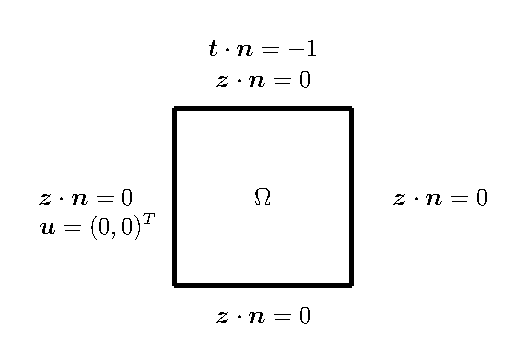
\includegraphics[width=0.5\textwidth]{canteliver_diag_crop.eps}}
  \subfloat[]{\label{fig:cantilever_plot}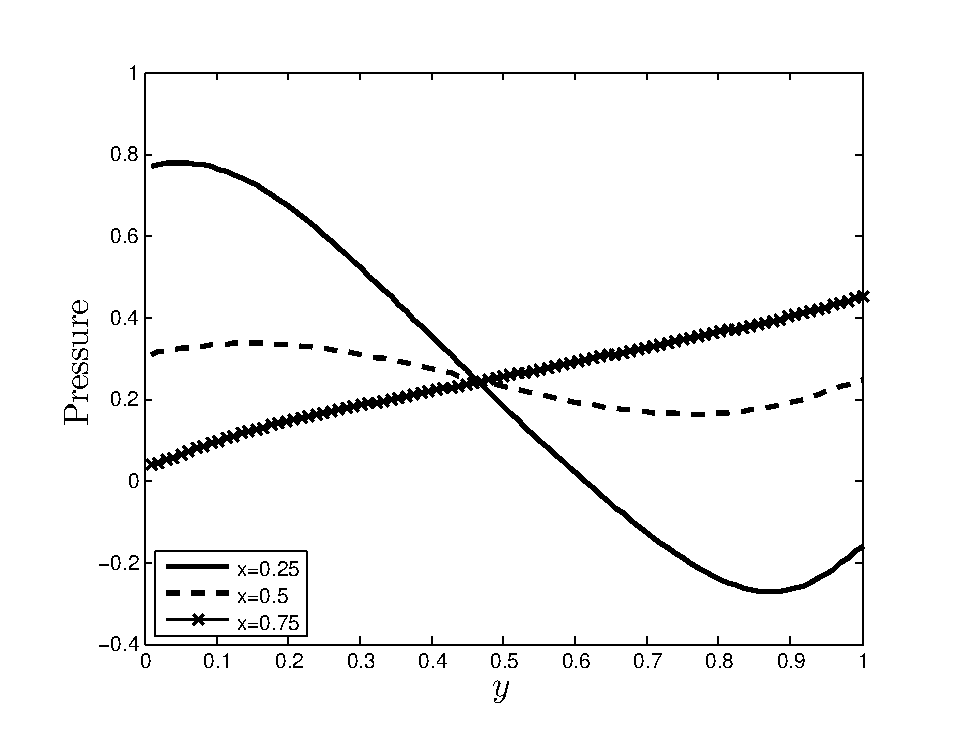
\includegraphics[width=0.5\textwidth]{cantilever_plot.eps}}
\caption{(a) Boundary conditions for the cantilever bracket problem. (b) Pressure solution of the cantilever bracket problem at $t=0.005$.}
\end{figure}

%%%%%%%%%%%%%%%%%%%%%%%%%%%%%%%%%%%%%%%%%%%%%%%%%%%%%%%%%%%%%%%%%%%%%%%%%%%%%%%%%%%%%%%%%%%%%%%%%%%%
%     3D unconfined compression stress relaxation
%%%%%%%%%%%%%%%%%%%%%%%%%%%%%%%%%%%%%%%%%%%%%%%%%%%%%%%%%%%%%%%%%%%%%%%%%%%%%%%%%%%%%%%%%%%%%%%%%%%%

\subsection{3D unconfined compression stress relaxation}
\label{sec:unconfined}
In this test, a cylindrical specimen of porous tissue is exposed to a prescribed displacement in the axial direction while left free to expand radially. (Note that the two plates are not explicitly modelled in the simulation, but are realised through displacement boundary conditions.) After loading the tissue, the displacement is held constant while the tissue relaxes in the radial direction due to interstitial fluid flow through the radial boundary. For the special case of a cylindrical geometry \cite{armstrong1984analysis} found a closed-form analytical solution for the radial displacement $u$ given by
\begin{equation}
 \frac{u}{a}(a,t)=\epsilon_{0}\left[ \nu + (1-2\nu)(1-\nu) \sum^{\infty}_{n=1}\frac{\exp{( -\alpha_n^{2} \frac{M k t}{a^{2}}}) }{ \alpha_{n}^{2}(1-\nu)^{2}-(1-\nu) }  \right].
\end{equation}
where $\alpha_n$ are the solutions to the characteristic equation $J_{1}(x)-(1-\nu)xJ_{0}(x)/(1-2\nu)=0,$ where $J_{0}$ and $J_{1}$ are Bessel functions, $\epsilon_{0}$ is the amplitude of the applied axial strain, $a$ is the radius of the cylinder, and $t_{g}$ is the characteristic time of diffusion (relaxation) $t_{g}= a^{2}/M k$, where $M=\lambda + 2\mu$ is the P-wave modulus of the elastic solid skeleton, and $k$ is the permeability.


%We computed the solution to $T=10\mbox{s}$  using a time step $\Delta t=0.1\mbox{s}$ and the radial displacement predicted by our implementation (Figure \ref{fig:anal_unconfined_plot}) using a value of $\delta=0.001$ gives a root mean squared error of $6.7\times 10^{-4}$ against the analytical solution provided by \cite{armstrong1984analysis}, and yields a stable solution. The same test problem has also been used to verify other poroelastic software such as FEBio \cite{maas2012febio}.
The analytical solution available for this test problem describes the displacement of the outer radius which is directly dependent on the amount of mass in the system since the porous medium is assumed to be incompressible and fully saturated. It is therefore an ideal test problem for analyzing the effect that the added stabilization term has on the conservation of mass. In Figure \ref{fig:anal_unconfined_plot} we can see that for large values of $\delta$ the numerical solution loses mass faster and comes to a steady state that has less mass than the analytical solution. This is a clear limitation of the method and the stability parameter therefore needs to be chosen carefully. However, for 3D problems $\delta$ can be chosen to be very small so this effect is negligible, as can be seen in Figure \ref{fig:anal_unconfined_plot} for a stable value of $\delta=0.001$.

\begin{figure}[H]
  \centering
  \subfloat[]{\label{fig:unconfined_diag}\includegraphics[width=0.4\textwidth]{unconfined_diag.eps}}
  \subfloat[]{\label{fig:unconfined_sim}\includegraphics[width=0.5\textwidth]{unconfined.eps}}
  \label{fig:animals}
\caption{ (a) Sketch of the test problem. The porous medium is being compressed between two smooth impervious plates. The frictionless plates permit the porous medium to expand in order to conserve volume and then to gradually relax as the fluid seeps out radially. (b) Pressure field solution at $t=5$, using a mesh with 28160 tetrahedra.}
\end{figure}
 \begin{figure}[H]
\begin{center}
\includegraphics[width=0.6\linewidth]{unconfined_results_delta.eps}
\caption{Normalized radial displacement versus normalized time calculated using the analytical
solution, and using the proposed numerical method with different values of $\delta$. At $t=0$ the radial expansion is half of the axial compression indicating the instantaneous incompressibility of the poroelastic tissue. The final amount of tissue recoil depends on the intrinsic Poisson ratio of the tissue skeleton.}
\label{fig:anal_unconfined_plot}
\end{center}
\end{figure}


\section{Conclusion}
The local pressure jump stabilization method \cite{burman2007unified} is commonly used to solve the Stokes or Darcy equations using piecewise linear approximations for the velocities, and piecewise constant approximations for the pressure variable. The main contribution of this chapter has been to extend these ideas to three-field poroelasticity. We have presented a stability result for the discretized equations that guarantees the existence of a unique solution at each time step, and derived an energy estimate which can be used to prove weak convergence of the solution to the discretized system to the solution to the continuous problem as the mesh parameters tend to zero. We also derived an optimal error estimate which includes an error for the fluid flux in its natural $H{div}$ norm. We have also presented numerical experiments in 2D and 3D that illustrate the convergence of the method, the effectiveness of the method in overcoming spurious pressure oscillations, and the added mass effect of the stabilization term.


%\begin{abstractchap}
% %\begin{comment}
\begin{abstract}
{A stabilized conforming mixed finite element method for the three-field (displacement, fluid flux and pressure) poroelasticity problem is deveeloped and analyzed. We use the lowest possible approximation order, namely piecewise constant approximation for the pressure, and piecewise linear continuous elements for the displacements and fluid flux. By applying a local pressure jump stabilization term to the mass conservation equation we ensure stability and avoid pressure oscillations. Importantly, the discretization leads to a symmetric linear system. For the fully discretized problem we prove existence and uniqueness, an energy estimate and an optimal a-priori error estimate, including an error estimate for the divergence of the fluid flux. Numerical experiments in 2D and 3D illustrate the convergence of the method, show the effectiveness of the method to overcome spurious pressure oscillations, and evaluate the added mass effect of the stabilization term.}
%Keywords
{poroelasticity; stabilized mixed finite elements; well-posedness;
a-priori error estimates.}
\end{abstract}
%\end{comment}

%\end{abstractchap}

%\input{/users/lorenzb/Dphil/poroelasticity_papers/ima_submission/introduction_jcam}
%\input{/users/lorenzb/Dphil/poroelasticity_papers/ima_submission/themodel_jcam}
%\input{/users/lorenzb/Dphil/poroelasticity_papers/ima_submission/bilinearforms_jcam}
%\input{/users/lorenzb/Dphil/poroelasticity_papers/ima_submission/cont_formulations_jcam}
%\input{/users/lorenzb/Dphil/poroelasticity_papers/ima_submission/full_discrete_model_jcam}
%\input{/users/lorenzb/Dphil/poroelasticity_papers/ima_submission/stability_fully_discrete_jcam}
%\input{/users/lorenzb/Dphil/poroelasticity_papers/ima_submission/energy_fully_discrete_jcam}
%\input{/users/lorenzb/Dphil/poroelasticity_papers/ima_submission/apriori_jcam}
%\section{Implementation}
Since the system of equations (\ref{eqn:full_model}) is highly nonlinear, its solution requires a scheme such as Newton's method. In chapter \ref{chap:large_fem} a finite element scheme using Newton's method for the solution of the poroelastic equations valid in large deformations (\ref{eqn:simple_mixture_model}) has already been presented. In this chapter we adopt the same finite element scheme as presented in chapter \ref{chap:large_fem} for solving the poroelastic equations and expand the linear system (discretized linearization) to include additional matrices required for solving the fluid network and its coupling to the poroelastic medium (equations (\ref{eqn:mixture_mass_reform_full},\ref{eqn:tree_flow},\ref{eqn:tree_mass},\ref{eqn:pressure_coupling})). This results in a monolithic coupling scheme that ensures good convergence even for problems with strong coupling interactions between the poroelastic medium and the fluid network (see section \ref{sec:constriction}). For details on how the stiffness matrix $\boldsymbol{K}$ (discretized linearization of the full lung model (\ref{eqn:full_model})), and the residual vector $\boldsymbol{R}$ are built, see section \ref{sec:fem_appendix}. To solve the nonlinear poroelastic problem using Newton's method at a particular time step, we perform the the steps already described in algorithm \ref{algo:newton}. We set the relative tolerance to be $\mbox{TOL}=10^{-4}$. For the subsequent numerical results shown in section \ref{sec:numerical_results}, a maximum of $5$ Newton iterations were required to solve each time step.






\subsection{Discrete coupling of the fluid network to the poroelastic model}
\label{sec:coupling_appendix}
If we discretize the space using triangles and employ a piecewise constant pressure approximation (one node at the center of each element), the resulting coupling for the simple 2D example (Figure \ref{fig:domains_cont}) is shown in Figure \ref{fig:coupling_disc1}. Once we refine the mesh (Figure \ref{fig:coupling_disc2}), the discretized division of subdomains tends to the subdivision of the original problem (Figure \ref{fig:domains_cont}).
%
The $i$th discretized subdomain $\Omega_{t}^{i}$ is defined as the set of elememts, $E$, closest to the position of the $i$th inlet, denoted by $\mbox{pos}(P_{di})$. 
\begin{equation}
\Omega_{t}^{i} := \left\lbrace E \in \Omega_{t} : ||\mbox{pos}(P_{di}) - \mbox{cent}(E) || <  ||\mbox{pos}(P_{dk}) - \mbox{cent}(E) ||, \;k=1,2...,N \,, k \neq i \right\rbrace,
 \label{discrete_subdomain_definition}
\end{equation} 
where $ \mbox{cent}(E)$ denotes the centroid of an element.
%This highlights that the numerical approximation is not mesh dependent, provided a fine enough mesh discretisation is used.
\begin{figure}[h]
\centering
\subfloat[]{\begin{tikzpicture}[scale=1.35]
  %Coarse discretisation
  \draw[semithick,fill=black!2,fill opacity=0.5] 
    (0,1) to (1,2) to  (2,1) to (0,1) ;
  \draw[semithick,fill=black!2,fill opacity=0.5] 
    (0,1) to (1,0) to  (2,1) to (0,1) ; 
  \draw[semithick,fill=black!2,fill opacity=0.5] 
    (1,2) to (2,1) to  (3,2) to (1,2) ;
   \draw[semithick,fill=black!2,fill opacity=0.5] 
    (1,0) to (2,1) to  (3,0) to (1,0) ;
    \draw[semithick,fill=black!25,fill opacity=0.5] 
    (2,1) to (3,2) to  (4,1) to (2,1) ;
  \draw[semithick,fill=black!25,fill opacity=0.5] 
    (2,1) to (3,0) to  (4,1) to (2,1) ;

   %TREE
  \draw[line width=2pt] (2.2,1.9) -- (2.2,2.5);
  \draw[line width=2pt] (3.4,0.7) -- (2.2,1.9);
  \draw[line width=2pt] (2,0.7) -- (2.2,1.9);
    		     	
	%Labelling
	\draw (3.2,0.55) node {$P_{d2}$};
	\draw (3.1,1.4) node {  $\Omega_{t}^{2}$};
	\draw (2,0.5) node {$P_{d1}$};
	\draw (1,1.4) node {  $\Omega_{t}^{1}$};	
\end{tikzpicture}
\label{fig:coupling_disc1}
}
\subfloat[]{\begin{tikzpicture}[scale=1.35]

  %Top left tri
  \draw[semithick,fill=black!2,fill opacity=0.5] 
    (0,1) to (0.3,1.7141) to  (1,1) to (0,1) ;
   \draw[semithick,fill=black!2,fill opacity=0.5] 
    (1,1) to (1.5,1.5) to  (2,1) to (1,1) ;
  \draw[semithick,fill=black!2,fill opacity=0.5] 
    (0.3,1.7141) to (1,2) to  (1.5,1.5) to (0.3,1.7141) ;
    \draw[semithick,fill=black!2,fill opacity=0.5] 
    (0.3,1.7141) to (1.5,1.5) to  (1,1) to (0.3,1.7141) ;
    
   %Top right tri
   \draw[semithick,fill=black!25,fill opacity=0.5] 
    (2.5,1.5) to (3,2) to  (3.7,1.7141) to (2.5,1.5) ;
       \draw[semithick,fill=black!25,fill opacity=0.5] 
    (2.5,1.5) to (3.7,1.7141) to  (3,1) to (2.5,1.5) ;
  \draw[semithick,fill=black!2,fill opacity=0.5] 
    (2,1) to (2.5,1.5) to  (3,1) to (2,1) ;
   \draw[semithick,fill=black!25,fill opacity=0.5] 
   (3,1) to (3.7,1.7141) to  (4,1) to (3,1) ;

   %Bottom left
   \draw[semithick,fill=black!2,fill opacity=0.5] 
    (0,1) to (0.3,0.2859) to  (1,1) to (0,1) ;
   \draw[semithick,fill=black!2,fill opacity=0.5] 
    (1,1) to (1.5,0.5) to  (2,1) to (1,1) ;
  \draw[semithick,fill=black!2,fill opacity=0.5] 
    (0.3,0.2859) to (1,0) to  (1.5,0.5) to (0.3,0.2859) ;
    \draw[semithick,fill=black!2,fill opacity=0.5] 
    (0.3,0.2859) to (1.5,0.5) to  (1,1) to (0.3,0.2859) ;

 
    %Bottom right
  \draw[semithick,fill=black!25,fill opacity=0.5] 
    (2.5,0.5) to (3,0) to  (3.7,0.2859) to (2.5,0.5) ;
       \draw[semithick,fill=black!25,fill opacity=0.5] 
    (2.5,0.5) to (3.7,0.2859) to  (3,1) to (2.5,0.5) ;
  \draw[semithick,fill=black!2,fill opacity=0.5] 
    (2,1) to (2.5,0.5) to  (3,1) to (2,1) ;
   \draw[semithick,fill=black!25,fill opacity=0.5] 
   (3,1) to (3.7,0.2859) to  (4,1) to (3,1) ;
 
  %Bottom middle - to do
  \draw[semithick,fill=black!2,fill opacity=0.5] 
    (1.5,0.5) to (2,1) to  (2.5,0.5) to (1.5,0.5) ;
  \draw[semithick,fill=black!2,fill opacity=0.5] 
    (1,0) to (1.5,0.5) to  (2,0) to (1,0) ;
  \draw[semithick,fill=black!2,fill opacity=0.5] 
    (2,0) to (2.5,0.5) to  (3,0) to (2,0) ;
  \draw[semithick,fill=black!2,fill opacity=0.5] 
    (1.5,0.5) to (2,0) to  (2.5,0.5) to (1.5,0.5) ;
    
  %Top Middle
  \draw[semithick,fill=black!2,fill opacity=0.5] 
    (1.5,1.5) to (2,1) to  (2.5,1.5) to (1.5,1.5) ;
  \draw[semithick,fill=black!2,fill opacity=0.5] 
    (1,2) to (1.5,1.5) to  (2,2) to (1,2) ;
  \draw[semithick,fill=black!2,fill opacity=0.5] 
    (2,2) to (2.5,1.5) to  (3,2) to (2,2) ;
  \draw[semithick,fill=black!2,fill opacity=0.5] 
    (1.5,1.5) to (2,2) to  (2.5,1.5) to (1.5,1.5) ; 
   %TREE
   \draw[line width=2pt] (2.2,1.9) -- (2.2,2.5);
   \draw[line width=2pt] (3.4,0.7) -- (2.2,1.9);
   \draw[line width=2pt] (2,0.7) -- (2.2,1.9);	
	%Labelling
	%\draw (3.2,0.55) node {$P_{d2}$};
	\draw (3.1,1.4) node {  $\Omega_{t}^{2}$};
	%\draw (2,0.5) node {$P_{d1}$};
	\draw (1,1.4) node {  $\Omega_{t}^{1}$};	
\end{tikzpicture}
\label{fig:coupling_disc2}
}
\caption{(a) Coupling between the discretized domain and the fluid network using a piecewise constant pressure approximation for the example shown in Figure \ref{fig:domains_cont}. (b) Coupling between the discretized domain and the fluid network after mesh refinement.} 
\label{fig:coupling}
\end{figure}



\subsection{Finite element matrices}
\label{sec:fem_appendix}
For the fully-coupled large deformation poroelastic fluid network model we need to solve the linear system $\boldsymbol{K}(\mathfrak{u}_{i}^{n}) \change \mathfrak{u}_{i+1}^{n} = - \boldsymbol{R}(\mathfrak{u}_{i}^{n},\mathfrak{u}^{n-1})$ at each Newton iteration. This can be expanded as
%
 \begin{equation*}
 \begin{bmatrix}
   \mathbf{K}^{e} & 0 & \mathbf{B}^{T} & 0  & 0 & 0 & 0&  0\\
  0 & \mathbf{M} & \mathbf{B}^{T} & \mathbf{L}^{T}  & 0& 0 & 0&  0\\
 -  \mathbf{B} & -\Delta t \mathbf{B} & \mathbf{J} & 0 & 0 & 0&  0 & -\Delta t \mathbf{G}^{T} \\
 0 & \mathbf{L} & 0 & 0 & 0 &  0 & 0 &  0\\
 0 & 0 & 0& 0 &  \mathbf{T}_{11}   &   \cdots & \cdots& \mathbf{T}_{14} \\
 0 & 0 & 0& 0 & \vdots\  & &     & \vdots\\
0 & 0 & 0& 0 & \mathbf{T}_{31}  & \cdots &\cdots & \mathbf{T}_{34}\\
 0 & 0 & \mathbf{G} & 0 & 0 &  -\mathbf{X}  &  0&  0 \\
 \end{bmatrix}
 \begin{bmatrix}
  \change\mathbf{u}^{n} \\
  \change\mathbf{z}^{n} \\
 \change\mathbf{p}^{n}  \\
\change\mathbf\Lambda^{n}  \\
\change\mathbf{P}^{n}  \\
\change\mathbf{P}^{n}_{d}  \\
\change\mathbf{Q}^{n}  \\
\change\mathbf{Q}_{d}^{n}  \\
 \end{bmatrix}=-
 \begin{bmatrix}
  \boldsymbol{r}_{1} \\
  \boldsymbol{r}_{2} \\
 \boldsymbol{r}_{3} -\Delta t \mathbf{G}^{T} \mathbf{Q}_{d}^{n} \\
0 \\
0 \\
0 \\
0 \\
\mathbf{G} \mathbf{p}^{n} - \mathbf{X} \mathbf{P}^{n}_{d}
 \end{bmatrix},
 \end{equation*}
 where we have defined the following matrices and vectors:
 \begin{equation*}
  \boldsymbol{K}^{e}=[\boldsymbol{a}_{kl}], \;\; \boldsymbol{k}^{e}_{kl}=\int_{{\Omega_{t} }} \boldsymbol{E}^{T}_{k}\boldsymbol{D}(\boldsymbol{u}^{n}_{i})\boldsymbol{E}_{l}+  (\nabla \boldsymbol{\phi}_{k})^{T}\boldsymbol{\sigma}_{e}(\boldsymbol{u}^{n}_{i})\nabla \boldsymbol{\phi}_{l}  \; dv,
 \end{equation*}
 \begin{equation*}
  \boldsymbol{M}=[\boldsymbol{m}_{kl}], \;\; \boldsymbol{m}_{kl}=\int_{{\Omega_{t} }} \perminv(\boldsymbol{u}^{n}_{i})  \boldsymbol{\phi}_{k} \cdot  \boldsymbol{\phi}_{l} \; dv,
 \end{equation*}
\begin{equation*}
  \boldsymbol{B}=[\boldsymbol{b}_{kl}], \;\; \boldsymbol{b}_{kl}=-\int_{{\Omega_{t} }}  {\psi}_{k} \nabla \cdot \boldsymbol{\phi}_{l} \; dv,
 \end{equation*}
 \begin{equation*}
  \boldsymbol{J}=[\boldsymbol{j}_{kl}], \;\; \boldsymbol{j}_{kl}= \delta \sum_{K} \int_{\partial k \backslash \partial {\Omega_{t} }} h_{\partial K} [{\psi}_{k}][{\psi}_{k}] \;ds.
 \end{equation*}
  \begin{equation*}
  \boldsymbol{r}_{1}=[\boldsymbol{r}_{1i}], \;\; \boldsymbol{r}_{1i}=  \int_{{\Omega_{t}}} \left(\boldsymbol{\sigma}_{e}(\boldsymbol{u}^{n}_{i})-p^{n}_{i} \boldsymbol{I} \right) : \nabla \boldsymbol{\phi}_{i}  - {\rho}(\boldsymbol{u}^{n}_{i})  \boldsymbol{\phi}_{i}\cdot \boldsymbol{f}  \; dv - \int_{\Gamma_{t}}    \boldsymbol{\phi}_{i} \cdot \boldsymbol{t}_{N}    \; ds,
 \end{equation*}
  \begin{equation*}
  \boldsymbol{r}_{2}=[\boldsymbol{r}_{2i}], \;\; \boldsymbol{r}_{2i}= \int_{{\Omega_{t}}}  \perminv(\boldsymbol{u}^{n}_{i}) \boldsymbol{\phi}_{i} \cdot \boldsymbol{z}^{n}_{i}  -{p}^{n}_{i} \nabla \cdot \boldsymbol{\phi}_{i} -{\rho^{f}}(\boldsymbol{u}^{n}_{i}) \boldsymbol{\phi}_{i}\cdot \boldsymbol{f}  \; dv ,
 \end{equation*}
  \begin{multline*}
  \boldsymbol{r}_{3}=[\boldsymbol{r}_{3i}], \;\; \boldsymbol{r}_{3i}= \int_{{\Omega_{t}}}  {\psi}_{i}   \nabla \cdot  \left( {\boldsymbol{u}^{n}_{i}-\boldsymbol{u}^{n-1}} \right) +  \Delta t {\psi}_{i}  \nabla \cdot \boldsymbol{z}^{n}_{i}   - \Delta t{\psi}_{i} g  \; dv \\ + \delta \sum_{K} \int_{\partial k \backslash \partial {\Omega_{t} }} h_{\partial K} [{\psi}_{i}]\left[{{p}^{n}_{i}-{p}^{n-1}}\right] \;ds.
 \end{multline*}
  \begin{equation*}
  \mathbf{L}=[\mathbf{l}_{ij}], \;\; \mathbf{l}_{ij}=\int_{\Omega} {\epsilon}_{i}  \mathbf{\phi}_{j} \cdot \normal,
 \end{equation*}
\begin{equation*}
\mathbf{X}=[\mathbf{x}_{ij}], \; \mathbf{x}_{ij} := \left\lbrace
  \begin{array}{l l}
    1 &  \text{if $||\mbox{pos}(P_{di}) - \mbox{cent}(E_{j}) || <  ||\mbox{pos}(P_{dk}) - \mbox{cent}(E_{j}) ||, k=1,2...,N \;, k \neq i $},\\
    0 &  \text{otherwise},
  \end{array} \right.
\end{equation*}
%with $\mbox{cent}(E_{j})$ denoting the center of element $E_{j}$.
 \begin{equation*}
  \mathbf{G}=[\mathbf{g}_{ij}], \;\; \mathbf{g}_{ij}=\int_{\Omega} \mathbf{x}_{ij}   \frac{ \mathbf{\phi}_{j}}{|E_{j}|},
 \end{equation*}
$\mathbf{T}$ represents the matrix entries required for the fluid network.\newline

Here $\boldsymbol{\epsilon}_{k}$ are scalar valued linear basis functions such that the Lagrangian multiplier vector at the $i$th iteration can be written as $\boldsymbol{\Lambda}^{n}_{i}= \sum_{k=1}^{n_{\Lambda}}\boldsymbol{\Lambda}^{n}_{i,k}\boldsymbol{\epsilon}_{k}$, and $\mbox{cent}(E_{j})$ denotes the centroid of the $j$th element. All other terms have already been defined in section \ref{sec:newton}.


%\input{/users/lorenzb/Dphil/poroelasticity_papers/ima_submission/simulations}
%\section{Conclusion}
%Stabilized low-order methods can offer significant computational advantages over higher order approaches. In particular, one can employ meshes with fewer degrees of freedom, fewer Gauss points, and simpler data structures. The additional stabilization terms can also improve the convergence properties of iterative solvers. These factors become crucial when considering large-scale, coupled, three-dimensional problems. There has also been a need for a method that is able to overcome both pressure oscillations due to the mixed finite element formulation not satisfying the LBB (inf-sup) condition and due to steep pressure gradients in the solution.

The main contribution of this chapter has been to extend the local pressure jump stabilization method \cite{burman2007unified}, already applied to three-field linear poroelasticity in chapter \ref{chap:linear_poro} to the large deformation case. Thus, the proposed scheme is built on an existing scheme, for which rigorous theoretical results about the stability and optimal convergence have been proven, and numerical experiments have confirmed its ability to overcome spurious pressure oscillations. Due to the discontinuous pressure approximation, sharp pressure gradients due to changes in material coefficients or boundary layer solutions can be captured reliably, circumventing the need for severe mesh refinement. Also, the addition of the stabilization term introduces minimal additional computational work, can be assembled locally on each element using standard element information, and leads to a symmetric addition to the original system matrix, thus preserving any existing symmetry. As the numerical examples have demonstrated, the stabilization scheme is robust and leads to high-quality solutions.


%This is (below) basically outline of paper sections
%We first derived the general poroelasticity equations and then reformulated the model to arrive at the standard quasi-static poroelasticity formulation. We then outlined the linearization and subsequent discretization of the equations, along with a detailed descritpion of the resulting Newton algorithm. Finally we presented numerical experiments in 3D that verify the method against analytical solutions and illustrate the effectiveness of the method to capture stepp pressure gradients due to changes in material parameters of boundary layer solutions.


%In this work we have proposed a stabilization scheme to allow
%for the use of Q4P4 elements, though the same scheme can also
%be applied to simplicial elements and three-dimensions. The method
%employed has several appealing features. It requires only a
%minor modification of standard finite element codes, and adds
%little additional computational cost to the assembly routines. All
%necessary computations can be performed at the element level
%using standard shape-function information, and no higher-order
%derivatives or stress-recovery techniques must be employed. It also
%leads to a symmetric modification of the system






%%Large deformation poroelasticity 
\chapter{A stabilized finite element method for nonlinear poroelasticity valid in large deformations}
\label{chap:large_fem}

\section{Introduction}
In chapter \ref{chap:linear_poro}, we developed a stabilized, low-order, mixed finite-element method for the fully saturated, incompressible, poroelasticity equations, in the linear, small deformation case. In this chapter we extend this work to the nonlinear, large deformation case.

In section \ref{sec:large_model}, we recall the large deformation quasi-static incompressible poroelastic model. In section \ref{sec:fem} we present the stabilized nonlinear finite-element method, and provide some implementation details in section \ref{sec:implementation}. In section \ref{sec:results}, we present a range of 3D  numerical experiments to verify the accuracy of the method and illustrate its ability to reliably capture steep pressure gradients.
\section{The model}
\label{sec:large_model}
%To arrive at the simplified, quasi-static, fully saturated incompressible large deformation poroelasticity formulation, we will introduce some additional model assumptions% that will be justified later (see other document)
%, and introduce the fluid flux variable given by
%\begin{equation}
%  \boldsymbol{z}=\phi(\boldsymbol{v}^{f}-\boldsymbol{v}^{s}).
%\label{eqn:relative_fluid}
%\end{equation}
Following \cite{ateshian2010finite} and \cite{almeida1998finite}, we recall the governing equations (\ref{eqn:simple_mixture_model}) for a fully saturated, incompressible poroelastic model  valid in large deformations. The problem is to find $\boldsymbol{\chi}(\boldsymbol{X},t)$,  $\boldsymbol{z}(\boldsymbol{x},t)$ and $p(\boldsymbol{x},t)$ such that
\begin{equation}
\label{eqn:mixture_momentum_reform}
\begin{gathered}\begin{aligned}
-\nabla \cdot( \boldsymbol{\sigma}_{e} -p\boldsymbol{I}) &= \rho\boldsymbol{f} \\
{\perm^{-1}\boldsymbol{z}} + \nabla p &=  \rho^{f}\boldsymbol{f}  \\
\nabla \cdot (\boldsymbol{v}^{s} + \boldsymbol{z} )  &= g  \\
\boldsymbol{\chi} &= \boldsymbol{X}+\boldsymbol{u}_{D}  \\
(\boldsymbol{\sigma}_{e}-p\boldsymbol{I})\boldsymbol{n} &= \boldsymbol{t}_{N}  \\
\boldsymbol{z} \cdot \boldsymbol{n} &= {q_{D}}  \\
p &= p_{D}  \\
\boldsymbol{\chi}(0) &= \boldsymbol{X} + \boldsymbol{u}^{0}
\end{aligned}\end{gathered}
\;
%\left .
\begin{gathered}\begin{aligned}
&\mbox{in} \; \Omega_{t}, \\
&\mbox{in} \; \Omega_{t}, \\
&\mbox{in} \; \Omega_{t}, \\
&\mbox{on} \; \Gamma_{d}, \\
&\mbox{on} \; \Gamma_{t}, \\
&\mbox{on} \; \Gamma_{f}, \\
&\mbox{on} \; \Gamma_{p}, \\
&\mbox{in} \; \Omega_{0}.
\end{aligned}\end{gathered}
%\qquad \right \}
\end{equation}

where $\boldsymbol{v}^{s}(\boldsymbol{x},t)=  \pderiv{}{t}\boldsymbol{\chi}(\boldsymbol{X},t)$.
\begin{rem}
It is a  straightforward extension to include the solid inertia $\boldsymbol{a}^{s}$ which can the be discretized using a Newmark scheme, see e.g. \cite{chapelle2010poroelastic}, \cite{li2004dynamics}, \cite{sauter2010robust}.
\end{rem}

\section{The stabilized finite element method}
\label{sec:fem}
For ease of presentation, we will assume all Dirichlet boundary conditions are homogeneous, ie., $\boldsymbol{u}_{D} = {\bf 0}, {q_{D}} = 0, p_{D}=0$.  %


%%%%%%%%%%%%%%%%%%%%%%%%%%%%%%%%%%%%%%%%%%%%%%%%%%%%%%%%%%%%%%%%%%%%%%%%%%%%%%%%%%%%%%%%%%%%%%%%%%%%
%     Weak formulation
%%%%%%%%%%%%%%%%%%%%%%%%%%%%%%%%%%%%%%%%%%%%%%%%%%%%%%%%%%%%%%%%%%%%%%%%%%%%%%%%%%%%%%%%%%%%%%%%%%%%

\subsection{Weak formulation}
\label{sec:weak_forms}
To keep the notation similar to chapter \ref{chap:linear_poro}, we solve for the displacement $\boldsymbol{u}(\boldsymbol{X},t) = \boldsymbol{\chi}(\boldsymbol{X},t)-\boldsymbol{X}$ rather than the deformation map $\boldsymbol{\chi}(\boldsymbol{X},t)$, and define the following spaces for deformed location, fluid flux and pressure respectively,
\begin{eqnarray*}
\dispspace &=& \{ \dispcont \in (H^{1} (\Omega))^d :\dispcont= {\bf 0} \;\mbox{on} \;\Gamma_{D} \}, \\
\fluxspace &=& \{ \fluxcont \in H_{div}(\Omega):\fluxcont \cdot \normal = 0 \;\mbox{on} \;\Gamma_{F} \}, \\
\pspace    &=& \left\{
  \begin{array}{l l}
    L^{2}(\Omega)     &\; \text{if} \; \Gamma_{n} \cup \Gamma_{p} \neq \emptyset \\
    L^{2}_{0}(\Omega) &\; \text{if} \;\Gamma_{n} \cup \Gamma_{p} = \emptyset,
  \end{array} \right \},
\end{eqnarray*}
where
$L^{2}_{0}(\Omega) = \left\{ q \in L^{2}(\Omega) : \int_{\Omega} q\;\mbox{d}x=0\right\}$.
We combine these to construct the mixed solution space
\begin{equation*}
\mixedspace = \left\{ \dispspace
  \times \fluxspace  \times  \pspace \right\}.
\end{equation*}


We make use of the identity $\nabla \cdot ( \boldsymbol{\sigma}_{e} \dispconttest)= \nabla \cdot \boldsymbol{\sigma}_{e} \cdot \dispconttest -  \boldsymbol{\sigma}_{e} : \nabla \dispconttest $, and  the symmetry of $\boldsymbol{\sigma}_{e}$ to yield the following continuous weak problem. Find $\dispcont(\boldsymbol{X},t) \in \dispspace$, $\fluxcont(\boldsymbol{x},t) \in \fluxspace$, and $\pcont(\boldsymbol{x},t) \in \mathcal{L}(\Omega)$ for any time $t\in[0,T]$ such that
\begin{equation}
\label{eqns:weak_cont_system}
%\left .
\begin{aligned}
\int_{\Omega_{t}}  \boldsymbol{\sigma}_{e}
                : \nabla^{S} \dispconttest    \; dv
 - \int_{\Omega_{t}}  \pcont   \nabla \cdot \dispconttest  \; dv
&= \int_{\Omega_{t}}  \rho \boldsymbol{f} \cdot \dispconttest  \; dv
 + \int_{\Gamma_{t}} \boldsymbol{t}_{N} \cdot \dispconttest  \; ds \; \forall \dispconttest\in \dispspace, \\
\int_{\Omega_{t}} \perminv \fluxcont \cdot \fluxconttest \; dv
  - \int_{\Omega_{t}}  \pcont  \nabla \cdot\fluxconttest \; dv
&= \int_{\Omega_{t}} \rho^{f} \boldsymbol{f} \cdot \fluxconttest \; dv \; \forall\fluxconttest\in \fluxspace,  \\
\int_{\Omega_{t}} \pconttest \nabla \cdot  \dispconttime \; dv
 + \int_{\Omega_{t}} \pconttest \nabla \cdot \fluxcont \; dv
&= \int_{\Omega_{t}} g   \pconttest \; dv  \; \forall \pconttest \in \mathcal{L}(\Omega).
\end{aligned}
%\quad \right \}
\end{equation}
Here $ \nabla^{S} \boldsymbol{s}=\frac{1}{2}\left( \nabla \boldsymbol{s} + (\nabla \boldsymbol{s})^{T} \right)$ for some vector $\boldsymbol{s}$.

%%%%%%%%%%%%%%%%%%%%%%%%%%%%%%%%%%%%%%%%%%%%%%%%%%%%%%%%%%%%%%%%%%%%%%%%%%%%%%%%%%%%%%%%%%%%%%%%%%%%
%     The fully discrete model
%%%%%%%%%%%%%%%%%%%%%%%%%%%%%%%%%%%%%%%%%%%%%%%%%%%%%%%%%%%%%%%%%%%%%%%%%%%%%%%%%%%%%%%%%%%%%%%%%%%%

\subsection{The fully discrete model}
\label{sec:fully_discrete}

Let $\mathcal{T}^{h}$ be a partition of $\Omega$ into non-overlapping elements $K$, where $h$ denotes the size of the largest element in $\mathcal{T}^{h}$ and assume that the partition is quasi-uniform. We define the following finite element spaces,
\begin{eqnarray*}
\dispspacedisc &=& \left\{ \dispdisc  \in C^{0}(\Omega): \dispdisc |_{K} \in P_{1}(K) \ \forall K \in \mathcal{T}^{h}, \dispdisc  = 0 \; \mbox{on} \;\Gamma_{D} \right\},  \\
\fluxspacedisc &=&\left\{ \fluxdisc  \in C^{0}(\Omega): \fluxdisc |_{K} \in P_{1}(K) \ \forall K \in \mathcal{T}^{h},  \fluxdisc \cdot \normal = 0 \; \mbox{on} \;\Gamma_{F} \right\}, \\
\pspacedisc &=& \left\{
  \begin{array}{l l}
    \left\{ \pdisc: \pdisc |_{K} \in P_{0}(K) \ \forall K \in \mathcal{T}^{h} \right\} & \; \text{if $\Gamma_{n} \cup \Gamma_{p} \neq \emptyset$}\\
    \left\{ \pdisc: \pdisc |_{K} \in P_{0}(K), \int_{\Omega}  \pdisc =0 \ \forall K \in \mathcal{T}^{h}\right\} & \; \text{if $\Gamma_{n} \cup \Gamma_{p}=\emptyset$}
  \end{array} \right. ,
\end{eqnarray*}
where $P_{0}(K)$ and $P_{1}(K)$ are respectively the spaces of constant and linear polynomials on $K$. We partition $[0,T]$ into $N$ evenly spaced non-overlapping regions $(t_{n-1}, t_n]$, $n=1,2,\dots, N$ , where $t_n-t_{n-1} = \Delta t$. For any sufficiently smooth function $v(t,x)$ we define $v^n(x) = v(t_n,x)$  and the discrete time derivative by $v_{\Delta t}^{n} := \frac{v^{n}-v^{n-1}}{\Delta t}$.

The fully discrete weak problem is: For $n = 1,2, \ldots,N$, find $\dispdisc^{n} \in \dispspacedisc$, $\fluxdisc^{n} \in \fluxspacedisc$ and $\pdisc^{n} \in \pspacedisc $ such that


\begin{multline}
\label{eqns:weak_disc_system}
\int_{\Omega_{t}}\boldsymbol{\sigma}_{e,h}^{n}
                 : \nabla^{S} \dispdisctest \; dv
 - \int_{\Omega_{t}}  \pdisc^{n}   \nabla \cdot \dispdisctest  \; dv
= \int_{\Omega_{t}}  \rho \boldsymbol{f}^{n} \cdot \dispdisctest  \; dv
 + \int_{\Gamma_{t}} \boldsymbol{t}_{N}^{n} \cdot \dispdisctest  \; ds \;
   \forall \dispdisctest \in \dispspacedisc, \\
\int_{\Omega_{t}} \perminv \fluxdisc^{n} \cdot \fluxdisctest \; dv
  - \int_{\Omega_{t}}  \pdisc^{n}  \nabla \cdot\fluxdisctest \; dv
= \int_{\Omega_{t}} \rho^{f} \boldsymbol{f}^{n} \cdot \fluxdisctest \; dv \; \forall\fluxdisctest\in \fluxspacedisc,  \\
\int_{\Omega_{t}} \pdisctest \nabla \cdot  \dispdisctimen \; dv
 + \int_{\Omega_{t}} \pdisctest \nabla \cdot \fluxdisc^{n} \; dv + J(\pdisctimediscn,\pdisctest)
= \int_{\Omega_{t}} g^{n}   \pdisctest \; dv  \; \forall \pdisctest \in \pspacedisc.
\end{multline}
 

%The stabilization term is
%\begin{equation}
%J(\pcont,\pconttest)= \delta \sum_{K} \int_{\partial K \backslash \partial \Omega} h_{\partial K} [\pcont][\pconttest] \;\mbox{d}s.
%\end{equation}
%Here $\delta$ is a stabilization parameter that is independent of $h$ and $\Delta t $.  Here $ h_{\partial K} $ denotes the size (diameter) of an element edge in 2D or face in 3D, and $[\cdot]$ is the jump across an edge or face (taken on the interior edges only). %We will see in the numerical results, section \ref{sec:results} that the convergence is not sensitive to $\delta$. 



%\begin{multline}
%\int_{\Omega_{t}}  \nabla \cdot ( \frac{\Delta\dispdisc}{\Delta t } +  \cdot \Delta\fluxdisc ) \cdot \pdisctest  \;dv + %\frac{\delta}{\Delta t} \sum_{K} \int_{\partial k \backslash \partial \Omega} h_{\partial K} [\Delta \pdisc][\pdisctest] %\;{d}s \\ = \int_{\Omega_{t}}  \nabla \cdot ( \overline{\dispdisctimedisc} +  \cdot \overline{\fluxdisc} ) \cdot \pdisctest - g %\cdot \pdisctest \; dv  +  \delta \sum_{K} \int_{\partial k \backslash \partial \Omega} h_{\partial K} %[\overline{\pdisctimedisc
%}][\pdisctest] \;{d}s  \;\; \;\; \forall \pdisctest\in \pspacedisctest.
%\end{multline}

%Comment about straight forward extension to keep solid acceleration, using commonly used newmark scheme and linearization from forcing term.

%\subsection{Existence of a unique solution}

%This particular element is commonly used for ‘mixed’ finite element
%analysis in the infinitesimal regime, and passes the LBB condition for infinitesimal deformation [58].



%%%%%%%%%%%%%%%%%%%%%%%%%%%%%%%%%%%%%%%%%%%%%%%%%%%%%%%%%%%%%%%%%%%%%%%%%%%%%%%%%%%%%%%%%%%%%%%%%%%%
%     Newton's method
%%%%%%%%%%%%%%%%%%%%%%%%%%%%%%%%%%%%%%%%%%%%%%%%%%%%%%%%%%%%%%%%%%%%%%%%%%%%%%%%%%%%%%%%%%%%%%%%%%%%

%outline: linearize the virtual work statement and then discretize
\subsection{Newton's Method}
\label{sec:newton_method}

Since the system of equations (\ref{eqns:weak_disc_system}) is highly nonlinear, its solution requires a scheme such as Newton's method. With Newton's method, an improved solution is obtained from a linear approximation of the nonlinear equation at an already computed solution. This first order Taylor expansion corresponds in finite element applications to the linearization of the weak form, and can be obtained by the directional derivative, explained in section \ref{sec:linearization}. Let $\solntrip^{n}=\{ \dispdiscn, \fluxdiscn, \pdiscn \} $ denote the solution vector at a particular time step, $\solnchangetrip=\{ \dispcontchange,  \fluxcontchange, \pcontchange \} $ denote the solution increment vector, and $\testtrip=\{ \dispdisctest, \fluxdisctest, \pdisctest \} $ the corresponding vector of test functions. Then the nonlinear system of equations (\ref{eqns:weak_disc_system}) can be recast in the form
\begin{equation}
 G(\solntrip,\testtrip)=0,
  \label{eqn:G_zero}
\end{equation}
where
\begin{multline}
G(\solntrip,\testtrip)=
\int_{\Omega_{t}}  \boldsymbol{\sigma}^{n}_{e,h}
                :  \nabla^{S} \dispdisctest 
- \pdiscn  \nabla\cdot \dispdisctest  \\
+ \int_{\Omega_{t}}\perminv \fluxdiscn \cdot \fluxdisctest
- \pdiscn  \nabla \cdot \fluxdisctest + \pdisctest\nabla \cdot ( {\dispdisctimediscn} +  \fluxdiscn ) \;dv  + J(\pdisctimediscn,\pdisctest)\\
- \int_{\Omega_{t}} \rho \boldsymbol{f}^{n}  \cdot \dispdisctest
+ \rho^{f} \boldsymbol{f}^{n} \cdot \fluxdisctest
+ g \pdisctest \; dv
- \int_{\Gamma_{t}}   \boldsymbol{t}_{N}^{n}  \cdot \dispdisctest  \; ds.
 \label{eqn:G_defintion}
\end{multline}
Considering a trial solution $ \solnattrip$, equation (\ref{eqn:G_zero}) can now be linearized in the direction of an increment $\solnchangetrip$ at $\solnattrip$ as
\begin{equation}
 G(\solnattrip,\testtrip) + DG(\solnattrip,\testtrip)[ \solnchangetrip] =0,
\end{equation}
or
\begin{equation}
 DG(\solnattrip,\testtrip)[ \solnchangetrip]= - G(\solnattrip,\testtrip),
\end{equation}
which essentially is Newton's method (see algorithm \ref{algo:newton} for the fully discrete version).

\subsubsection{Linearization}
\label{sec:linearization}
In biphasic tissue problems, it is common to approximate the tangent by taking the nonlinear elasticity term as the only nonlinearity present and ignoring the other nonlinearities \cite{un2006penetration,white2008stabilized}. 


 %This approach has been implemented with success in \cite{un2006penetration}, \cite{oomens1987mixture}, \cite{almeida1997mixed} and also seems to be robust for our proposed method.
The dominant nonlinearity in (\ref{eqn:G_defintion}) is the elasticity term denoted by
\begin{equation}
{E}((\dispdiscn,\pdiscn) ,\dispdisctest)=\int_{\Omega_{t}}
 \boldsymbol{\sigma}^{n}_{e,h}: \nabla^{S} \dispdisctest -  \pdiscn  \nabla\cdot \dispdisctest \; dv.
\end{equation}
For Newton's method we require the directional derivative of ${E}(\dispdisc ,\dispdisctest)$ at a particular trial solution $ \overline{\dispdisc}$ in the direction $\dispcontchange$, given by (see \cite[section 3.5.3]{wriggers2008nonlinear})
\begin{equation}
\begin{gathered}\begin{aligned}
D{E}( (\overline{\dispdiscn}, \overline{\pdiscn}) ,\dispdisctest)[\dispcontchange]
&=\int_{\Omega_{t}} \nabla^{S} \dispdisctest : \overline{\mathbf\Theta^{n}_{h}} :
 \nabla^{S} \dispcontchange  \\
&+
\overline{\boldsymbol{\sigma}^{n}_{e,h}} : \left( (\nabla \dispcontchange)^{T} \cdot \nabla \dispdisctest \right) \; dv,
\end{aligned}\end{gathered}
\end{equation}
where $\overline{\mathbf{\Theta}^{n}_{h}}$ is the fully-discrete, fourth-order spatial tangent modulus tensor and $\overline{\boldsymbol{\sigma}^{n}_{e,h}}$ is the effective (elastic) stress tensor both evaluated at a trial solution $ \overline{\dispdiscn}$. Any variable with a bar above it will correspond to it being evaluated at a trial solution and will therefore be considered as a known quantity. In the fully discrete algorithm \ref{algo:newton}, this trial solution will correspond to the solution of the previous Newton step. The spatial tangent modulus tensor $\mathbf\Theta$, due to its complexity, is described in section \ref{sec:incremental_spatial}. For a detailed explanation and derivation see \cite{wriggers2008nonlinear,bonet1997nonlinear}. The approximate linearization of the nonlinear problem (\ref{eqn:G_zero}) is thus given by
\begin{equation}
\begin{gathered}\begin{aligned}
&DG(\solnattrip , \testtrip ) \solnchangetrip \\
&\approx \int_{\Omega_{t}}  \nabla^{S} \dispdisctest  : \overline{\mathbf \Theta^{n}_{h}} :
         \nabla^{S} \dispcontchange \\
&+ \overline{\boldsymbol{\sigma}_{e,h}} :
            \left( (\nabla \dispcontchange)^{T} \cdot \nabla \dispdisctest \right)
- \pcontchange  \nabla \cdot\dispdisctest \; dv \\
&+ \int_{\Omega_{t}}  \perminvat \fluxcontchange \cdot \fluxdisctest
- \pcontchange  \nabla\cdot \fluxdisctest \;dv
+  \int_{\Omega_{t}} \pdisctest\nabla \cdot \left( \frac{\dispcontchange}{\Delta t }
+  \fluxcontchange \right) \; dv + J(\pdisctimediscn,\pdisctest).
\end{aligned}\end{gathered}
\end{equation}


The fully discretized weak problem at each Newton step, to get an update for the approximate solution, is to find $ \dispcontchange \in \dispspacedisc$, $\fluxcontchange \in \fluxspacedisc$ and $\pcontchange \in \pspacedisc $ such that:

\begin{multline}
\label{eqn:newton_mass}
\int_{\Omega_{t}} \nabla^{S} \dispdisctest : \overline{\mathbf \Theta^{n}_{h}} : \nabla^{S} \dispcontchange  + \overline{\boldsymbol{\sigma}^{n}_{e,h}}:
            \left( (\nabla \dispcontchange)^{T} \cdot \nabla \dispdisctest \right)
 - {\pcontchange}  \nabla \cdot\dispdisctest \; dv \\+ \int_{\Omega_{t}}  \perminvat \fluxcontchange \cdot \fluxdisctest \; dv -  \pcontchange  \nabla \cdot \fluxdisctest \;dv \\+ \int_{\Omega_{t}} \pdisctest \nabla \cdot
       \left( \frac{\dispcontchange}{\Delta t } +  \fluxcontchange \right)  \;dv
+ J\left(\frac{ \pcontchange }{\Delta t},\pdisctest\right) \\
\quad = \int_{\Omega_{t}}
  \frac{1}{2} \overline{\boldsymbol{\sigma}^{n}_{e,h}}:
              \left( \nabla \dispdisctest + (\nabla \dispdisctest)^{T} \right)
- \overline{\pdiscn}  \nabla \cdot \dispdisctest  - \overline{\rho} \boldsymbol{f}^{n} \cdot \dispdisctest \; dv
- \int_{\Gamma_{t}}  \boldsymbol{t}_{N}^{n} \cdot \dispdisctest \; ds \; \\ + \int_{\Omega_{t}}  \perminvat \overline{\fluxdiscn} \cdot \fluxdisctest \; dv -     \overline{\pdiscn} \cdot \nabla \fluxdisctest \;dv -  \overline{\rho^{f}} \boldsymbol{f}^{n} \cdot \fluxconttest \; dv \;\; \\ + \int_{\Omega_{t}}
         \pdisctest \nabla \cdot ( \overline{\dispdisctimedisc} + \overline{\fluxdisc} )
         + J\left(\overline{\pdisctimedisc},\pdisctest\right) - g   \pdisctest \; dv  \;\; \forall (\dispdisctest,\fluxdisctest,\pdisctest )\in\dispspacedisc,\fluxspacedisc,\pspacedisctest.
\end{multline} 
We can rewrite this using more compact notation
\begin{equation}
 DG(\solnattrip,\testtrip) \solnchangetrip = - G(\solnattrip,\testtrip).
\end{equation}


%Finally we can now rewrite the problem of finding the Newton update as
%\begin{equation}
% \mathcal{K}(\solnattripdisc,\testtripdisc)[ \solnchangetripdisc]= - \mathcal{R}(\solnattripdisc,\testtripdisc),
%\end{equation}
%where $ \mathcal{K}(\solnattripdisc,\testtripdisc)[ \solnchangetripdisc]=DG_{h}(\solnattripdisc,\testtripdisc)[\solnchangetripdisc]+J(\pdisctimedisc,\pdisctest)[\solnchangetripdisc]$, and $ \mathcal{R}(\solnattripdisc,\testtripdisc)=G(\solnattripdisc,\testtripdisc)+J(\pdisctimedisc,\pdisctest)$.
%


%%%%%%%%%%%%%%%%%%%%%%%%%%%%%%%%%%%%%%%%%%%%%%%%%%%%%%%%%%%%%%%%%%%%%%%%%%%%%%%%%%%%%%%%%%%%%%%%%%%%
%     Implementation details
%%%%%%%%%%%%%%%%%%%%%%%%%%%%%%%%%%%%%%%%%%%%%%%%%%%%%%%%%%%%%%%%%%%%%%%%%%%%%%%%%%%%%%%%%%%%%%%%%%%%

\section{Implementation details}
\label{sec:implementation}


\subsection{Newton algorithm}
\label{sec:newton}
We will now let $\mathfrak{u}_{i}^{n}:=\{ \dispcont_{i}^{n}, \fluxcont_{i}^{n}, \pcont_{i}^{n} \} $ denote the fully discrete solution at the $i$th step within the Newton method at time $t^{n}$. To ease the notation, we have suppressed the lower case $h$, previously used to denote the spatial discretization. To solve the nonlinear poroelastic problem using Newton's method at a particular time step, we perform the following steps:
\begin{algorithm}[H]
\begin{algorithmic}[1]
  \caption{Fully discrete Newton's algorithm}
    \label{algo:newton}
  \STATE $i=0$
  \STATE $\mathfrak{u}_{0}^{n}=\{ \dispcont^{n-1}, \fluxcont^{n-1}, \pcont^{n-1} \} $
  \WHILE { $||\boldsymbol{R}(\mathfrak{u}_{i}^{n},\mathfrak{u}^{n-1})|| > \mbox{TOL} \; \& \; i < \mbox{ITEMAX}$  }
    \STATE Assemble  $\boldsymbol{R}(\mathfrak{u}_{i}^{n},\mathfrak{u}^{n-1})$ and $\boldsymbol{K}(\mathfrak{u}_{i}^{n})$
    \STATE Solve $\boldsymbol{K}(\mathfrak{u}_{i}^{n}) \xi\mathfrak{u}_{i+1}^{n} = -\boldsymbol{R}(\mathfrak{u}_{i}^{n},\mathfrak{u}^{n-1})$
    \STATE Compute $\mathfrak{u}_{i+1}^{n}=\mathfrak{u}_{i}^{n}+ \xi \mathfrak{u}_{i+1}^{n}$
    \STATE Update the mesh, $ \Omega_{t}= \boldsymbol{X} +\boldsymbol{u}_{i}^{n}$
    \STATE $i=i+1$
  \ENDWHILE
\end{algorithmic}
\end{algorithm}
%\footnotetext{%The deformation state is obtained within the nonlinear solution process by an update of the deformation state during the Newton iteration. This allows us to define to solve the equations in $\Omega_{t}$, or more precisely ${\Omega_{t}}_{i}$. Also note that all the basis functions (and their spatial derivatives) will change with every iteration.
%This method is known in the literature as an updated Lagrange formulation, see e.g. \cite{bathe1975finite} or \cite[chapter 3]{wriggers2008nonlinear}, however it should really be called an updated Eulerian formulation, since the current configuration is being updated during each Newton iteration. This method is also used by \cite{ateshian2010finite,white2008stabilized} to solve the large deformation poroelasticty problem.}
where $\boldsymbol{K}(\mathfrak{u}_{i}^{n})$ and $\boldsymbol{R}(\mathfrak{u}_{i}^{n},\mathfrak{u}^{n-1})$ are the matrix and vector representations of $DG(\mathfrak{u}_{i}^{n})$ and $G(\mathfrak{u}_{i}^{n},\mathfrak{u}^{n-1})$, respectively.
%\begin{equation}
%DG(\mathfrak{u}_{i}^{n}) \change \mathfrak{u}_{i+1}^{n} = - G(\mathfrak{u}_{i}^{n},\mathfrak{u}^{n-1}),
%\end{equation}
At each Newton iteration we solve the linear system
\begin{equation}
\boldsymbol{K}(\mathfrak{u}_{i}^{n}) \change \mathfrak{u}_{i+1}^{n} = - \boldsymbol{R}(\mathfrak{u}_{i}^{n},\mathfrak{u}^{n-1}),
\end{equation}
which can be expanded, and written as
 \begin{equation*}
 \begin{bmatrix}
  \boldsymbol{K}^{e} & 0 & \boldsymbol{B}^{T} \\
  0 & \boldsymbol{M} & \boldsymbol{B}^{T} \\
  -\boldsymbol{B} & -\Delta t \boldsymbol{B} &\boldsymbol{J}
 \end{bmatrix}
 \begin{bmatrix}
  \change \boldsymbol{u}^{n}_{i+1} \\
  \change{z}^{n}_{i+1} \\
 \change \boldsymbol{p}^{n}_{i+1}
 \end{bmatrix}= -
 \begin{bmatrix}
  \boldsymbol{r}_{1}(\boldsymbol{u}^{n}_{i},{p}^{n}_{i}) \\
  \boldsymbol{r}_{2}(\boldsymbol{u}^{n}_{i},\boldsymbol{z}^{n}_{i},{p}^{n}_{i})  \\
  \boldsymbol{r}_{3}(\boldsymbol{u}^{n}_{i},\boldsymbol{u}^{n-1},\boldsymbol{z}^{n}_{i},{p}^{n}_{i})
 \end{bmatrix},
 \end{equation*}
 where we have defined the following matrices:
 \begin{eqnarray*}
&&\boldsymbol{K}^{e}=[\boldsymbol{a}_{kl}], \;\; \boldsymbol{k}^{e}_{kl}=\int_{{\Omega_{t} }} \boldsymbol{E}^{T}_{k}\boldsymbol{D}(\boldsymbol{u}^{n}_{i})\boldsymbol{E}_{l}+  (\nabla \boldsymbol{\phi}_{k})^{T}\boldsymbol{\sigma}_{e}(\boldsymbol{u}^{n}_{i})\nabla \boldsymbol{\phi}_{l}  \; dv, \\
&&\boldsymbol{M}=[\boldsymbol{m}_{kl}], \;\; \boldsymbol{m}_{kl}
 =  \int_{{\Omega_{t} }} \perminv(\boldsymbol{u}^{n}_{i})  \boldsymbol{\phi}_{k} \cdot  \boldsymbol{\phi}_{l} \; dv, \\
&&\boldsymbol{B}=[\boldsymbol{b}_{kl}], \;\; \boldsymbol{b}_{kl}
 = -\int_{{\Omega_{t} }}  {\psi}_{k} \nabla \cdot \boldsymbol{\phi}_{l} \; dv, \\
&& \boldsymbol{J}=[\boldsymbol{j}_{kl}], \;\; \boldsymbol{j}_{kl}
= \delta \sum_{K} \int_{\partial k \backslash \partial {\Omega_{t} }} h_{\partial K} [{\psi}_{k}][{\psi}_{k}] \;ds. \\
&& \boldsymbol{r}_{1} = [\boldsymbol{r}_{1i}], \;\; \boldsymbol{r}_{1i}
=  \int_{{\Omega_{t}}} \left(\boldsymbol{\sigma}_{e}(\boldsymbol{u}^{n}_{i})-p^{n}_{i} \boldsymbol{I} \right) : \nabla \boldsymbol{\phi}_{i}
- {\rho}(\boldsymbol{u}^{n}_{i})  \boldsymbol{\phi}_{i}\cdot \boldsymbol{f}  \; dv - \int_{\Gamma_{t}}    \boldsymbol{\phi}_{i} \cdot \boldsymbol{t}_{N}    \; ds, \\
&& \boldsymbol{r}_{2} = [\boldsymbol{r}_{2i}], \;\; \boldsymbol{r}_{2i}= \int_{{\Omega_{t}}}  \perminv(\boldsymbol{u}^{n}_{i}) \boldsymbol{\phi}_{i} \cdot \boldsymbol{z}^{n}_{i}  -{p}^{n}_{i} \nabla \cdot \boldsymbol{\phi}_{i} -{\rho^{f}}(\boldsymbol{u}^{n}_{i}) \boldsymbol{\phi}_{i}\cdot \boldsymbol{f}  \; dv , \\
&& \boldsymbol{r}_{3} = [\boldsymbol{r}_{3i}], \;\; \boldsymbol{r}_{3i}= \int_{{\Omega_{t}}}  {\psi}_{i}   \nabla \cdot  \left( {\boldsymbol{u}^{n}_{i}-\boldsymbol{u}^{n-1}} \right)
+  \Delta t {\psi}_{i}  \nabla \cdot \boldsymbol{z}^{n}_{i}   - \Delta t{\psi}_{i} g  \; dv  \\
&& \hskip 5cm + \delta \sum_{K} \int_{\partial k \backslash \partial {\Omega_{t} }} h_{\partial K} [{\psi}_{i}]\left[{{p}^{n}_{i}-{p}^{n-1}}\right] \;ds.
 \end{eqnarray*}
Here $\boldsymbol{\phi}_{k}$ are vector valued linear basis functions such that the displacement vector at the $i$th iteration can be written as $\boldsymbol{u}^{n}_{i}= \sum_{k=1}^{n_{u}}\boldsymbol{u}^{n}_{i,k}\boldsymbol{\phi}_{k}$, with $\sum_{k=1}^{n_{u}}\boldsymbol{u}^{n}_{i,k}\boldsymbol{\phi}_{k} \in \dispspacedisc$. Similarly for the fluid flux vector we have $\boldsymbol{z}^{n}_{i}= \sum_{k=1}^{n_{z}}\boldsymbol{z}^{n}_{i,k}\boldsymbol{\phi}_{k}$, with $\sum_{k=1}^{n_{z}}\boldsymbol{z}^{n}_{i,k}\boldsymbol{\phi}_{k} \in \fluxspacedisc$. The scalar valued constant basis functions ${\psi}_{i}$ are used to approximate the pressure, such that $\boldsymbol{p}^{n}_{i}= \sum_{k=1}^{n_{p}}{p}^{n}_{i,k}{\psi}_{k}$, with $\sum_{k=1}^{n_{p}}{p}^{n}_{i,k}{\psi}_{k} \in \pspacedisc$. Also to aid the assembly of the fourth order tensor we have adopted the matrix voigt notation. In particular $\boldsymbol{D}$ is the matrix form of ${\spatialincremental}$, and $\boldsymbol{E}_{k}$ is the matrix version of $\nabla^{S}\boldsymbol{\phi}_{k}$, see (\ref{matrixvoigt}) and (\ref{eqn:sym_matrix}) for details.



\subsection{No-flux boundary condition}
\label{sec:no-flux}

We introduce a Lagrange multiplier $\Lambda$, to enforce the no-flux boundary condition $\boldsymbol{z}\cdot \normal = 0 $ along the boundary $\Gamma_{f}$. Let ${W}^{f}=\{ \Lambda \in H_{div}(\Gamma_{f},\mathbb{R}) \}$. The resulting modified continuous weak-form is now:
\begin{equation}
\begin{gathered}\begin{aligned}
G((\dispcont,\fluxcont,\pcont) ) , (\dispconttest,\fluxconttest,\pconttest) )
+ (\Lambda,\fluxconttest \cdot \normal )_{\Gamma_{f}}
& =0 \; \forall (\dispconttest,\fluxconttest,\pconttest) \in \dispspace, \fluxspace, \pspace,\\
(\fluxcont \cdot \normal,\lambdaconttest  )_{\Gamma_{f}} & =0, \; \forall \lambdaconttest \in {W}^{f}.
\end{aligned}\end{gathered}
\label{eqns:weak_cont_system_integrated}
\end{equation}
The discretization and implementation of this additional constraint is straightforward and results in a linear system with additional degrees of freedom for every node on $\Gamma_{f}$. The terms $(\Lambda,\fluxconttest \cdot \normal )_{\Gamma_{f}}$ and $(\fluxcont \cdot \normal,\lambdaconttest  )_{\Gamma_{f}}$ are nonlinear since the normal is a function of the displacement. However we have found that treating these terms as linear terms does not affect the convergence of the Newton algorithm. Alternatively these terms could be linearized as has been described in detail for the traction boundary condition, see \cite[section 4.2.5]{wriggers2008nonlinear}.







\section{Numerical results}
\label{sec:results}

We  present four numerical examples to test the performance of the proposed stabilized finite element method. The first two examples are from mechanobiology and geotechnical applications, the third is a swelling example that undergoes significant large deformations and the fourth is an application from respiratory physiology. For the implementation we used the C++ library libmesh \cite{kirk2007libmesh}, and the multi-frontal direct solver mumps \cite{amestoy2000multifrontal} to solve the resulting linear systems. For the strain energy law we chose a Neo-Hookean law taken from \cite[eqn. (3.119)]{wriggers2008nonlinear}, with the penalty term chosen such that $0\leq\phi<1$, namely

%from \cite[eqn. (3.119)]{wriggers2008nonlinear},
\begin{equation}
W(\bb{C})=\frac{\mu}{2}(\mbox{tr}(\boldsymbol{C})-3)+\frac{\lambda}{4}(J^{2}-1)-(\mu+\frac{\lambda}{2})\mbox{ln}(J-1+\phi_{0}).
\label{eqn:NeoHookean}
\end{equation}
For further discussion on strain energy laws for porelasticity we refer to \cite{chapelle2014general} and \cite{vuong2014general}. The material parameters $\mu$ and $\lambda$ in (\ref{eqn:NeoHookean}) can be related to the Young's modulus $E$ and the Poisson ratio $\nu$ by $\mu=E/(2(1+\nu))$ and  $\lambda=(E\nu)/((1+\nu)(1-2\nu))$. Details of the effective stress tensor and fourth-order spatial tangent modulus for this particular law can be found in \ref{sec:neo_example}. For the permeability law we chose
\begin{equation}
\perm_{0}(\boldsymbol{C})=k_{0}\boldsymbol{I}.
\end{equation}

%%%%%%%%%%%%%%%%%%%%%%%%%%%%%%%%%%%%%%%%%%%%%%%%%%%%%%%%%%%%%%%%%%%%%%%%%%%%%%%%%%%%%%%%%%%%%%%%%%%%
%     3D unconfined compression stress relaxation
%%%%%%%%%%%%%%%%%%%%%%%%%%%%%%%%%%%%%%%%%%%%%%%%%%%%%%%%%%%%%%%%%%%%%%%%%%%%%%%%%%%%%%%%%%%%%%%%%%%%

\subsection{3D unconfined compression stress relaxation}
\label{sec:unconfined}

In this test, a cylindrical specimen of porous tissue is exposed to a prescribed displacement in the axial direction while left free to expand radially. The original experiment involved a specimen of articular cartilage being compressed via impervious smooth plates as shown in Figure \ref{fig:unconfined_diag}. Note that the two plates are not explicitly modelled in the simulation, but are realised through displacement boundary conditions. After loading the tissue, the displacement is held constant and the tissue is allowed to relax in the radial direction. The fluid pressure was constrained to zero at the outer radial surface. The outer radial boundary is permeable and free-draining, the upper and lower fluid boundaries are impermeable and frictionless. The outer radius and height of the cylinder is $5mm$, whereas the axial compression is $0.01 mm$. The parameters used for the simulation can be found in Table \ref{tab:unconfined_parameters}. For the special case of a cylindrical geometry, \cite{armstrong1984analysis} provides a closed-form analytical solution for the radial displacement on the porous medium in response to a step loading function.

\begin{figure}[h]
  \centering
  \subfloat[]{\label{fig:unconfined_diag}\includegraphics[width=0.45\textwidth]{figures/unconfined_diag.eps}}
  \subfloat[]{\label{fig:unconfined_sim}\includegraphics[width=0.55\textwidth]{figures/unconfined_large.eps}}
  \label{fig:animals}
\caption{ (a) The test problem. (b) Pressure field at $t=200s$ using a mesh with 3080 tetrahedra.}
\end{figure}


\begin{table}[h]
\begin{center}
\scalebox{0.8}{
\begin{tabular}{ l c c c c }
\hline
Parameter    &  Description                     & Value  \\
\hline
$k$          & Dynamic permeability             & $10^{-3} \; \mbox{m}^{3}\,\mbox{s}\,\mbox{kg}^{-1}$  \\
$\nu$        & Poisson's ratio                  & $0.15$  \\
$E$          & Young's modulus                  & $1000$ $\mbox{kg}\,\mbox{m}^{-1}\,\mbox{s}^{-2}$  \\
\hline
$\Delta t$   & Time step used in the simulation & $4\,\mbox{s}$       \\
$T$          & Final time of the simulation     & $1000\,\mbox{s}$    \\
$\delta$   & Stabilization parameter          & $ 10^{-3}$ \\
\hline
\end{tabular}
}
\end{center}
\caption{Parameters used for the unconfined compression test problem.} \label{tab:unconfined_parameters}
\end{table}

The analytical solution for the radial displacement to this unconfined compression test is given by
\begin{equation}
 \frac{u}{a}(a,t)=\epsilon_{0}
 \left[ \nu + (1-2\nu)(1-\nu) \sum^{\infty}_{n=1}
        \frac{\exp{( -\alpha_n^{2} \frac{Mkt}{a^{2}}})}{\alpha_{n}^{2}(1-\nu)^{2}-(1-\nu)}  \right].
\end{equation}
Here $\alpha_n$ are the solutions to the characteristic equation, given by $J_{1}(x)-(1-\nu)xJ_{0}(x)/(1-2\nu)=0,$ where $J_{0}$ and $J_{1}$ are Bessel functions. We also have that $\epsilon_{0}$ is the amplitude of the applied axial strain, $a$ is the radius of the cylinder, and $t_{g}$ is the characteristic time of diffusion given by $t_{g}= a^{2}/M k$, where $M=\lambda + 2\mu$ is the P-wave modulus of the elastic solid skeleton, and $k$ is the permeability. The computed radial displacement (Figure \ref{fig:anal_unconfined_plot}) shows good agreement with the analytical solution provided by \cite{armstrong1984analysis}. The same problem has  been used to test other large deformation poroelastic software such as FEBio \cite{maas2012febio}. The effect of the stabilization parameter on the numerical solution has already been investigated in section \ref{sec:unconfined}.

%The analytical solution available for this test problem describes the displacement of the outer radius which is directly dependent on the amount of mass in the system since the porous medium is assumed to be incompressible and fully saturated. It is therefore an ideal test problem for analyzing the effect that the added stabilization term has on the conservation of mass. In Figure \ref{fig:anal_unconfined_plot} we can see that for large values of $\delta$ the numerical solution looses mass faster and comes to a steady state that has less mass than the analytical solution. This is a clear limitation of the method and the stability parameter therefore needs to be chosen carefully. However, for 3D problems $\delta$ can be chosen to be very small so this effect is negligible, as can be seen in Figure \ref{fig:anal_unconfined_plot} for a stable value of $\delta=0.001$.

\begin{figure}[h]
\begin{center}
\includegraphics[width=0.8\linewidth]{figures/unconfined_large_plot.pdf}
\caption{Radial expansion versus time comparing the analytical and numerical solutions with $\delta=0.001$.}
\label{fig:anal_unconfined_plot}
\end{center}
\end{figure}


%%%%%%%%%%%%%%%%%%%%%%%%%%%%%%%%%%%%%%%%%%%%%%%%%%%%%%%%%%%%%%%%%%%%%%%%%%%%%%%%%%%%%%%%%%%%%%%%%%%%
%     Terzaghi's problem
%%%%%%%%%%%%%%%%%%%%%%%%%%%%%%%%%%%%%%%%%%%%%%%%%%%%%%%%%%%%%%%%%%%%%%%%%%%%%%%%%%%%%%%%%%%%%%%%%%%%

\subsection{Terzaghi's problem}
\label{sec:Terzaghi}

This is a classical geomechanics example with an analytical solution, and has been used to investigate finite element pressure oscillations, caused by overshooting of the numerical solution near the boundary \cite{murad1994stability,white2008stabilized}. The domain consists of a porous column of unit height, bounded at the sides and bottom by rigid and impermeable walls. The top is free to drain ($p_{D}=0$) and has a downward traction force, $p_{0}$, applied to it. The boundary and initial conditions for this 1D problem can be written as
\begin{equation}
\begin{gathered}\begin{aligned}
t_{N} = -p_{0},\;\;p_{D}=0\;\;  &\mbox{on} \; x=0,\\
u=0,\;\;z=0,\;\; &\mbox{on} \; x=1, \\
u=0,\;\;z=0,\;\;p=0 \; &\mbox{in} \; (0,1).
\end{aligned}\end{gathered}
\label{eqn:compression}
\end{equation}
The analytical pressure solution, in non-dimensional form is given by
\begin{equation}
p^{*}=\sum_{n}^{\infty}\frac{2}{\pi(n+1/2)} \sin (\pi(n+1/2)) \exp^{-\pi(n+1/2)(\lambda+2\mu)k t}.
\end{equation}
When the poroelastic medium is subjected to the sudden loading, the saturating fluid undergoes an overpressurization. Subsequently this overpressure progressively vanishes, owing to the
diffusion process of the fluid towards the boundary at the top of the column, which remains drained. For a detailed explanation and derivation of this solution see \cite[section 5.2.2]{wriggers2008nonlinear}. We discretized the column using 60 hexahedra elements and solved the problem using the proposed stabilized low-order finite element method and a higher-order inf-sup stable finite element method that uses a piecewise linear pressure approximation. The simulation results of the pressure for the two methods, taken at $t=0.01s$ and $t=1s$ are shown in Figure \ref{fig:compression}. The material parameters used for the simulation can be found in Table \ref{tab:terzaghi_parameters}. At $t=0.01s$ the piecewise linear (continuous) approximation suffers from overshooting due to the boundary layer solution (Figure \ref{fig:pone001}). The proposed method, which uses a piecewise constant pressure approximation does not suffer from this problem, and captures the pressure boundary layer solution reliably (Figure \ref{fig:pzero001}). At $t=1s$ the boundary layer has grown and both the piecewise linear (Figure \ref{fig:pone1}) and piecewise constant (Figure \ref{fig:pzero1}) approximation yield satisfactory results.

\begin{table}[h]
\begin{center}
\scalebox{0.8}{
\begin{tabular}{ l c c c c }
\hline
Parameter     &  Description                     & Value  \\
\hline
$k_{0}$       & Dynamic permeability             & $10^{-5} \; \mbox{m}^{3}\,\mbox{s}\,\mbox{kg}^{-1}$  \\
$\nu$         & Poisson ratio                    & $0.25$  \\
$E$           & Young's modulus                  & $100$ $\mbox{kg}\,\mbox{m}^{-1}\,\mbox{s}^{-2}$  \\
\hline
$\Delta t$    & Time step used in the simulation & $0.01\,\mbox{s}$    \\
$T$           & Final time of the simulation     & $1\,\mbox{s}$    \\
$\delta$    & Stabilization parameter          & $2\times10^{-5}$ \\
\hline
\end{tabular}
}
\end{center}
\caption{Parameters used for Terzaghi's problem. \label{tab:terzaghi_parameters}}
\end{table}

\begin{figure}[H]
  \centering
  \subfloat[]{\label{fig:pone001} \includegraphics[width=0.5\textwidth]{figures/pone001.eps}}
  \subfloat[]{\label{fig:pzero001}\includegraphics[width=0.5\textwidth]{figures/pzero001.eps}} \newline
  \subfloat[]{\label{fig:pone1}   \includegraphics[width=0.5\textwidth]{figures/pone1.eps}}
  \subfloat[]{\label{fig:pzero1}  \includegraphics[width=0.5\textwidth]{figures/pzero1.eps}}
\caption{(a) Pressure at $t=0.01s$ using a continuous linear pressure approximation. (b) Pressure at $t=0.01s$ using a discontinuous piecewise constant approximation. (c) Pressure at $t=1s$ using a continuous linear pressure approximation. (d) Pressure at $t=1s$ using a discontinuous piecewise constant approximation. \label{fig:compression}}

\end{figure}

%%%%%%%%%%%%%%%%%%%%%%%%%%%%%%%%%%%%%%%%%%%%%%%%%%%%%%%%%%%%%%%%%%%%%%%%%%%%%%%%%%%%%%%%%%%%%%%%%%%%
%     Swelling test
%%%%%%%%%%%%%%%%%%%%%%%%%%%%%%%%%%%%%%%%%%%%%%%%%%%%%%%%%%%%%%%%%%%%%%%%%%%%%%%%%%%%%%%%%%%%%%%%%%%%

\subsection{Swelling test}
\label{sec:swelling}

This  problem is similar to the one in \cite{chapelle2010poroelastic} and highlights the method's ability to reliably capture jumps in the pressure solution due to changes in material parameters. Given a unit cube of material, a fluid pressure gradient is imposed between the two opposite faces at $X=0$ and $X=1$. The pressure $p_{D}$ on the inlet face $X = 0$ is increased very rapidly from zero to a limiting value of $10 \mbox{kPa}$, i.e., $p_{D} = 10^{4} (1-\mbox{exp}(-t^{2}/0.25)) \;\mbox{Pa})$. On the outlet face $X = 1$, the pressure is fixed to be zero, $p_{D} =0$. There are no sources of sinks of fluid. A zero flux condition is applied for the fluid velocity on the four other faces ($Y=0,1, \;Z=0,1$). Normal displacements are required to be zero on the planes $X = 0$, $Y = 0$ and $Z = 0$.  The permeability of the cube $0 < X < 0.5, 0.5 < Y < 1, 0 < Z <0.5$ (1/8 of the volume of the unit cube) is smaller than in the rest of the domain by a factor of 500. The computational domain shown in Figure \ref{fig:swell_setup}, highlighting the region of reduced permeability. The parameters chosen for this test problem are shown in Table \ref{tab:parameters}.

Fluid enters the region from the inlet face and the material swells like a sponge, undergoing large deformation as shown in Figure (\ref{fig:swell_sim}). The evolution of the pressure and the Jacobian at the points at $(0,0,1)$, $(0.5,0,1)$ and $(1,0,1)$ in the reference configuration is shown in Figures (\ref{fig:swell_p}) and (\ref{fig:swell_j}) respectively. These position are indicated by the red, blue and green balls in Figure \ref{fig:swell_setup}. The pressure decreases roughly linearly with $x$, the increase in volume also follows a similar pattern.  The pressure and volume change at the point $(0,1,0)$ (black ball in Figure \ref{fig:swell_setup}) is also shown in Figures (\ref{fig:swell_p}) and (\ref{fig:swell_j}). Due to its reduced permeability this region is much slower to swell and achieve its ultimate equilibrium state and the fluid mainly flows around the area of reduced permeability, see Figure \ref{fig:swell_sim}. The steep pressure gradients at the boundary of the less permeable region seen in Figure \ref{fig:swell_sim} are well approximated by the piecewise constant (discontinuous) pressure space even on this relatively coarse discretization. Continuous pressure spaces would require a much finer discretization in this region.

\begin{figure}[H]
  \centering
  \subfloat[]{\label{fig:swell_setup}\includegraphics[width=0.45\textwidth]{figures/setup_balls.eps}}
  \subfloat[]{\label{fig:swell_sim}\includegraphics[width=0.6\textwidth]{figures/bigswell_1s.eps}}
  \caption{(a) Initial simulation setup. The grey cube represents the area of reduced permeability. The colored balls highlight the position of the points used for tracking the pressure and volume change during the simulation, shown in Figures \ref{fig:swell_p} and \ref{fig:swell_j}. (b) The deformed cube after $1s$. The pressure solution is plotted and the jumps in pressure at the interface between the high and low permeability regions can clearly be seen. The arrows illustrate the fluid-flux profile. \label{fig:animals_two} }

\end{figure}

\begin{table}[h]
\begin{center}
\scalebox{0.9}{
\begin{tabular}{ l c c }
\hline
Parameter    & Value \\
\hline
$k_{0}$      & $10^{-5} \; \mbox{m}^{3}\,\mbox{s}\,\mbox{kg}^{-1}$ \\
$\nu$        & $0.3$ \\
$E$          & $8000$ $\mbox{kg}\,\mbox{m}^{-1}\,\mbox{s}^{-2}$ \\
\hline
$\Delta t$   & $0.02\,\mbox{s}$     \\
$T$          & $20\,\mbox{s}$     \\
$\delta$   & $10^{-4}$     \\
\hline
\end{tabular}
}
\end{center}
\caption{Parameters used for the swelling test problem. \label{tab:parameters}}
\end{table}

\begin{figure}[H]
  \centering
  \subfloat[]{\label{fig:swell_p}\includegraphics[width=0.5\textwidth]{figures/swell_plong.eps}}
  \subfloat[]{\label{fig:swell_j}\includegraphics[width=0.5\textwidth]{figures/swell_jlong.eps}}
\caption{ Pressure (a) and volume change, $J$, (b) are plotted against time for four points, $(0,0,1)$ (red), $(0.5,0,1)$ (blue), $(1,0,1)$ (green), and $(1,0,1)$ (black) in the reference configuration. The position of these balls is also shown in Figure \ref{fig:swell_setup}. \label{fig:animals_three} }
\end{figure}



\section{Conclusion}
%Stabilized low-order methods can offer significant computational advantages over higher order approaches. In particular, one can employ meshes with fewer degrees of freedom, fewer Gauss points, and simpler data structures. The additional stabilization terms can also improve the convergence properties of iterative solvers. These factors become crucial when considering large-scale, coupled, three-dimensional problems. There has also been a need for a method that is able to overcome both pressure oscillations due to the mixed finite element formulation not satisfying the LBB (inf-sup) condition and due to steep pressure gradients in the solution.

The main contribution of this chapter has been to extend the local pressure jump stabilization method \cite{burman2007unified}, already applied to three-field linear poroelasticity in chapter \ref{chap:linear_poro} to the large deformation case. Thus, the proposed scheme is built on an existing scheme, for which rigorous theoretical results about the stability and optimal convergence have been proven, and numerical experiments have confirmed its ability to overcome spurious pressure oscillations. Due to the discontinuous pressure approximation, sharp pressure gradients due to changes in material coefficients or boundary layer solutions can be captured reliably, circumventing the need for severe mesh refinement. Also, the addition of the stabilization term introduces minimal additional computational work, can be assembled locally on each element using standard element information, and leads to a symmetric addition to the original system matrix, thus preserving any existing symmetry. As the numerical examples have demonstrated, the stabilization scheme is robust and leads to high-quality solutions.


%This is (below) basically outline of paper sections
%We first derived the general poroelasticity equations and then reformulated the model to arrive at the standard quasi-static poroelasticity formulation. We then outlined the linearization and subsequent discretization of the equations, along with a detailed descritpion of the resulting Newton algorithm. Finally we presented numerical experiments in 3D that verify the method against analytical solutions and illustrate the effectiveness of the method to capture stepp pressure gradients due to changes in material parameters of boundary layer solutions.


%In this work we have proposed a stabilization scheme to allow
%for the use of Q4P4 elements, though the same scheme can also
%be applied to simplicial elements and three-dimensions. The method
%employed has several appealing features. It requires only a
%minor modification of standard finite element codes, and adds
%little additional computational cost to the assembly routines. All
%necessary computations can be performed at the element level
%using standard shape-function information, and no higher-order
%derivatives or stress-recovery techniques must be employed. It also
%leads to a symmetric modification of the system




%\begin{abstractchap}
% %\begin{comment}
\begin{abstract}
{A stabilized conforming mixed finite element method for the three-field (displacement, fluid flux and pressure) poroelasticity problem is deveeloped and analyzed. We use the lowest possible approximation order, namely piecewise constant approximation for the pressure, and piecewise linear continuous elements for the displacements and fluid flux. By applying a local pressure jump stabilization term to the mass conservation equation we ensure stability and avoid pressure oscillations. Importantly, the discretization leads to a symmetric linear system. For the fully discretized problem we prove existence and uniqueness, an energy estimate and an optimal a-priori error estimate, including an error estimate for the divergence of the fluid flux. Numerical experiments in 2D and 3D illustrate the convergence of the method, show the effectiveness of the method to overcome spurious pressure oscillations, and evaluate the added mass effect of the stabilization term.}
%Keywords
{poroelasticity; stabilized mixed finite elements; well-posedness;
a-priori error estimates.}
\end{abstract}
%\end{comment}

%\end{abstractchap}

%\input{/users/lorenzb/Dphil/poroelasticity_papers/large_deformation/contents/review}
%\input{/users/lorenzb/Dphil/poroelasticity_papers/large_deformation/contents/overview}

%Don't need these
%\input{/users/lorenzb/Dphil/poroelasticity_papers/large_deformation/contents/intro_theory}
%\input{/users/lorenzb/Dphil/poroelasticity_papers/large_deformation/contents/continuum_mechanics_theory}
%\input{/users/lorenzb/Dphil/poroelasticity_papers/large_deformation/contents/mixture_theory}


%Keep these
%\input{/users/lorenzb/Dphil/poroelasticity_papers/large_deformation/contents/intro_fem}
%\input{/users/lorenzb/Dphil/poroelasticity_papers/large_deformation/contents/cont_weak_fem}
%\input{/users/lorenzb/Dphil/poroelasticity_papers/large_deformation/contents/discretized_fem}
%\input{/users/lorenzb/Dphil/poroelasticity_papers/large_deformation/contents/implementation_fem}
%\input{/users/lorenzb/Dphil/poroelasticity_papers/large_deformation/contents/simulations}
%\section{Conclusion}
%Stabilized low-order methods can offer significant computational advantages over higher order approaches. In particular, one can employ meshes with fewer degrees of freedom, fewer Gauss points, and simpler data structures. The additional stabilization terms can also improve the convergence properties of iterative solvers. These factors become crucial when considering large-scale, coupled, three-dimensional problems. There has also been a need for a method that is able to overcome both pressure oscillations due to the mixed finite element formulation not satisfying the LBB (inf-sup) condition and due to steep pressure gradients in the solution.

The main contribution of this chapter has been to extend the local pressure jump stabilization method \cite{burman2007unified}, already applied to three-field linear poroelasticity in chapter \ref{chap:linear_poro} to the large deformation case. Thus, the proposed scheme is built on an existing scheme, for which rigorous theoretical results about the stability and optimal convergence have been proven, and numerical experiments have confirmed its ability to overcome spurious pressure oscillations. Due to the discontinuous pressure approximation, sharp pressure gradients due to changes in material coefficients or boundary layer solutions can be captured reliably, circumventing the need for severe mesh refinement. Also, the addition of the stabilization term introduces minimal additional computational work, can be assembled locally on each element using standard element information, and leads to a symmetric addition to the original system matrix, thus preserving any existing symmetry. As the numerical examples have demonstrated, the stabilization scheme is robust and leads to high-quality solutions.


%This is (below) basically outline of paper sections
%We first derived the general poroelasticity equations and then reformulated the model to arrive at the standard quasi-static poroelasticity formulation. We then outlined the linearization and subsequent discretization of the equations, along with a detailed descritpion of the resulting Newton algorithm. Finally we presented numerical experiments in 3D that verify the method against analytical solutions and illustrate the effectiveness of the method to capture stepp pressure gradients due to changes in material parameters of boundary layer solutions.


%In this work we have proposed a stabilization scheme to allow
%for the use of Q4P4 elements, though the same scheme can also
%be applied to simplicial elements and three-dimensions. The method
%employed has several appealing features. It requires only a
%minor modification of standard finite element codes, and adds
%little additional computational cost to the assembly routines. All
%necessary computations can be performed at the element level
%using standard shape-function information, and no higher-order
%derivatives or stress-recovery techniques must be employed. It also
%leads to a symmetric modification of the system

%

%\begin{comment}

%%Coupled lung model
\chapter{A poroelastic-fluid-network model of the lung}
\label{chap:lung}
\section{Introduction}
The aim of this chapter is not to present the most complete or accurate ventilation or deformation lung model to date. Instead we aim to present a new methodology and highlight some of the modelling assumptions required for a poroelastic lung model. We hope that this model will in future be extended to include sophisticated flow models of the airways, more advanced constitutive laws that make use of additional imaging data to parametrize the model, and improved registration algorithms, to yield a more realistic and accurate full organ lung model.

The rest of this chapter is organized as follows. In section \ref{sec:model} we present the assumptions and define the mathematical lung model and describe its implementation. In section \ref{sec:model_generation} we describe the generation of the computational lung geometry and boundary conditions, and in section \ref{sec:numerical_results} we present numerical simulations of tidal breathing, and investigate the effect of airway constriction and tissue weakening. Finally in section \ref{sec:conclusion}, we conclude and outline future work to improve the current lung model.

\section{Lung model assumptions}
%\label{sec:model}
%
%
%\subsection{Model assumptions}
\label{sec:assumptions}
%
%We will begin by giving a review of the main modelling assumptions and how they might affect the model's ability to predict deformation and ventilation within healthy and diseased lungs.
%

\subsection{Approximating lung parenchyma using a poroelastic medium}

\noindent \newline \textbf{Averaging over the tissue:} One of the major assumptions is that we can approximate the lung parenchyma using a poroelastic continuum description. This makes our model computationally tractable and allows us to use the well established theory of poroelasticity to couple the air with the tissue.

The use of a continuum model can be further supported by looking at the different length scales and structures of the tissue. For the microscopic length scale denoted by $l$ of the parenchyma we will use the diameter of an alveolus that can be approximated to be $0.02 \; \mbox{cm}$ \cite{ochs2004number}. The macroscopic length scale $L$ can be taken to be the diameter of a segment which measures around $4\;\mbox{cm}$ of tissue. So the ratio of the different length scales is small i.e $\epsilon := \frac{l}{L} \approx 0.005 \ll 1$. This along with the assumption that the structure of an acinus is porous (see Figures \ref{fig:pores} and \ref{fig:honey}) and approximately periodic supports the use of averaging techniques over the tissue to obtain a continuum description  in the form of a poroelastic medium. To further simplify the poroelastic equations we assume that the poroelastic continuum can be described by a solid phase (blood and tissue) and a fluid phase (air), where both phases are assumed to be incompressible. The interaction between the fluid pressure and the deformation of the solid skeleton is assumed to obey the effective stress principle. Note that by averaging over the tissue we do not seek to model individual alveoli but introduce macroscopic parameters such as the permeability and elasticity coefficients. In general, lung diseases usually affect significant regions of alveoli (lung tissue), thus, by changing the macro-scale parameters over the affected area of tissue we are still able to model changes in the tissue due to disease.

\noindent \textbf{Ignoring blood flow:}\label{section:blood_flow} Apart from collagen, fibers and air the other major component in the lung is blood. The volume taken up by collagen and  elastin fibers is similar to the volume occupied by the capillaries filled with blood (illustrated in Figure \ref{fig:pores}). In fact, the space not occupied by air is about $7\%$ of the parenchymal volume and is made up of $50\%$ capillary blood and $50\%$ of collagen and elastin fibers \cite{WeichertThesis}. Also the density of blood is similar to the density of tissue and much larger than that of air ($ {1060 \;\mbox{kg}\,\mbox{m}}^{-3}\gg  {1.18 \;\mbox{kg}\,\mbox{m}}^{-3}$). Since the capillaries are constantly filled with blood and the density of blood is similar to that of alveolar tissue we will make the simplifying assumption that the blood is simply part of the tissue (solid phase) and thus ignore accelerations and any redistribution of blood during breathing.

\noindent \textbf{Assuming incompressibility of the solid and the fluid:} Blood and tissue can be assumed to be incompressible. Under physiological conditions, air can also be assumed to be incompressible \cite{ismail2013coupled}.

\noindent \textbf{Ignoring solid inertia forces:}
\label{section:inertia} Simple calculations considering the sinusoidal motion of tissue near the diaphragm during normal breathing yield an estimate of $0.02\, \mbox{ms} ^{-2}$ for the maximum acceleration of lung parenchyma. Compared to the acceleration of gravity this is negligible, and it is therefore reasonable to ignore the inertia forces in the tissue.

\noindent \textbf{Ignoring fluid inertia forces:}
The fluid's Reynolds number in the lower airways that form part of the lung parenchyma, has been estimated to be around $1$ to $0.01$ \cite{pedley1970prediction}. Due to this relatively low Reynolds number we choose to ignore fluid inertia forces in the poroelastic medium. %\cite{ben2006simplified} also showed in their whole lung model that inertia forces can be neglected during quiet breathing.

\noindent \textbf{Ignoring viscous forces in the fluid:}\label{section:viscous_forces}
A dimensional analysis shows that the viscous stress in the fluid is small compared to the drag forces between the fluid and the porous structure, when the ratio of the different length scales is small \cite{markert2007constitutive}. We will therefore neglect the fluid viscous stress implying that the fluid behaves more or less inviscid within the porous structure.

%The magnitude of the viscous stress in the fluid $\left|\left|\nabla \bb{\sigma}_{visc}\right|\right|$ within a poroelastic medium can be evaluated according to \cite{coussy2004poromechanics} as $\left|\left|\nabla \bb{\sigma}_{visc}\right|\right|= \frac{\phi \mu^{f}}{l L} \left|\left|\bb{v}^{f} - \bb{v}^{s} \right|\right|$,
%where $l$ and $L$ are the microscopic and macroscopic characteristic length scales, respectively. This can be balanced with the order of magnitude of  $\left|\left| \frac{\phi^{2}}{\boldsymbol{k}}  \left(\bb{v}^{f} - \bb{v}^{s}\right)  \right|\right|$ that describes the viscous resistance opposed by the shear stress to the fluid flow from the drag at the internal walls of the porous network. To see whether the viscous forces play an important role we take the ratio between these two forces% as is done in section 3.3.1 of \cite{coussy2004poromechanics}
%\begin{equation*}
%  \left|\left|\nabla \bb{\sigma}_{visc}\right|\right| / \left|\left| \frac{\phi^{2}}{\boldsymbol{k}}  \left(\bb{v}^{f} - \bb{v}^{s}\right)  \right|\right|=\frac{\mu_{f} \boldsymbol{k} }{ \phi l L}.
%  \label{viscous_balance}
%\end{equation*}
%Using parameter estimates for healthy human tissue found in Table \ref{tab:lung_sim_parameters}, and the previous estimates of the length scales, we get a non-dimensional value for (\ref{viscous_balance}) of about $0.002 \ll 1$, indicating that viscous forces are insignificant. However, if we were to consider diseased states such as emphysema, where large areas of lung tissue completely break down leaving big holes, it could be argued that the permeability here increases by large amounts that would also cause the above estimate to increase, and suggest that in this case viscous forces could well play an important role, making it important to include them in our model. For simplicity we will choose to ignore this viscous stress for now but it may be included it in a future version of the model by replacing the Darcy flow model with a Brinkman, or even a Stokes flow model for big holes, where the homogenization assumption of a porous structure is not valid.
%\newline

%\noindent \textbf{Constitutive laws:}
%For simplicity we use an isotropic hyperelastic strain energy law to model the tissue.
%%
%%An isotropic strain energy law has already successfully been applied to model the tissue deformation in the healthy lung \cite{tawhai2009supine}.
%%
%Note that for diseased cases such as emphysema or fibrosis this isotropic assumption may become invalid. We also assume that the permeability of the tissue is isotropic. Again the assumption of an isotropic permeability may well become invalid during disease. With the increasing availability of detailed imaging data on the structure of the lung along with further modelling work on constitutive laws for lung tissue, anisotropic laws should be used in the future.
%
\begin{comment}
\begin{figure}[h]
  \centering
\subfloat[]{\label{fig:pores}\includegraphics[width=0.35\textwidth,height=2in]{figures/aveolarPores_BerkeleyLungLabLungtour.png}}  \subfloat[]{\label{fig:honey}\includegraphics[width=0.35\textwidth,height=2in]{figures/TB_to_aveolarduct_BerkeleyLungLabtour.png}}
\caption{(a) Alveoli in an alveolar duct. The dark round openings are pores between alveoli. The alveolar wall is quite thin and contains a network of capillaries. The average diameter of one alveoli is $0.2\;\mbox{mm}$. (b) Transition from terminal bronchiole to alveolar duct, from conducting airway to oxygen transfer area, diameter of terminal bronchiole is $0.5 \;\mbox{mm}$. Images are reproduced from \cite{lunglabshort}.
 }
   \label{fig:acinar_units}
\end{figure}
%
\end{comment}

\subsection{Approximating the airways using a fluid network model}
%
In order to make the coupled model computationally feasible we assume that a simple laminar flow model can describe the air flow in the airways and we make the common {Poiseuille flow assumption}. This flow assumption is also made in \cite{Swan2012,leary2014effects} where the air flow in a whole airway tree, from trachea down to the final bronchioles was assumed to be governed by Poiseuille flow.  Diseases affecting the airway tree can be modelled effectively by changing resistance (airway radius) parameters in the network flow model.

\section{Mathematical model}
\label{section:lung_model}
%We will now introduce the quasi-static fully incompressible poroelasticity equations, used for modelling the lung parenchyma, a simple fluid network model to model the airway tree, and outline how these two parts are coupled together.

\subsection{A poroelastic model for lung parenchyma} 
Having made the assumptions in section \ref{sec:assumptions} for the tissue we are left with the large deformation quasi-static incompressible poroelastic model (\ref{eqn:simple_mixture_model}).%
\subsubsection{Constitutive laws.}
\label{sec:constitutive}
To close the poroelastic model for the tissue (\ref{eqn:simple_mixture_model}) we need to choose constitutive laws for the permeability and strain energy. We will use the same permeability law that has already been proposed in \cite{kowalczyk1994modelling} to model lung parenchyma,
\begin{equation}
\bb{k}_{0} = {k}_{0} \left( J \frac{  \phi  }{\phi_{0}} \right)^{2/3} \boldsymbol{I}.
\label{eqn:perm_law}
\end{equation}
%
Exponential strain energy laws for lung parenchyma exist, for example the popular law by \cite{fung1975stress}. However little is known about how the constants in these laws should be interpreted and altered to model weakening of the tissue in an diseased state. Further, the constants in these laws are thought to have no physical meaning \cite{tawhai2009supine}. To make the interpretation of the elasticity constants and dynamics of the model as simple as possible we chose a Neo-Hookean law taken from \cite{wriggers2008nonlinear}, with the penalty term chosen such that $0\leq\phi<1$,
%
%from \cite[eqn. (3.119)]{wriggers2008nonlinear},
\begin{equation}
W(\bb{C})=\frac{\mu}{2}(\mbox{tr}(\boldsymbol{C})-3)+\frac{\lambda}{4}(J^{2}-1)-(\mu+\frac{\lambda}{2})\mbox{ln}(J-1+\phi_{0}).
\label{eqn:Neo_Hookean}
\end{equation}
The material parameters $\mu$ and $\lambda$ can be related to the more familiar Young's modulus $E$ and the Poisson ratio $\nu$ by $\mu=\frac{E}{2(1+\nu)}$ and  $\lambda=\frac{E\nu}{(1+\nu)(1-2\nu)}$. The values of these constants for modelling lung tissue have been investigated \cite{zhang2004technical,werner2009patient,de1981model} and are shown in Table \ref{tab:lung_sim_parameters}.


\subsection{A network flow model for the airway tree}
The flow rate $Q_{i}$ through the $ith$ pipe segment in the fluid network is given by the pressure-flow relationship
\begin{equation}
 \label{pois_flow_eqn}
 P_{i,1} - P_{i,2} = R_{i} Q_{i},
\end{equation}
where $R_{i}=\frac{8l\mu_{f}}{\pi r^{4}}$ is the Poiseuille flow resistance of a pipe segment ($r$ is the radius, $l$ is the length of the pipe, $\mu_{f}$ is the dynamic viscosity) and $P_{i, 1}$ and $P_{i,2}$ are the pressures at the proximal and distal nodes of the pipe segment, respectively. We also have conservation of flow at branches such that
\begin{equation}
 Q_{i}  = \sum_{Q_{i,j} \in Q_{i}} Q_{i,j},
\end{equation}
where $Q_{i,j}$ are the flow rates of the children branches of the $i$th flow segment. The outlet pressure of the fluid network is set using the boundary condition $P_{0}=\hat{P}$.



\subsubsection{Coupling the fluid network to the poroelastic model.}
We introduce subdomains to identify the region of the domain that is supplied with fluid from a specific branch of the fluid network and returns fluid through that branch. We construct an approximate Voronoi tesselation based on the terminal end locations of the fluid network, so that the $i$th subdomain $\Omega_{t}^{i}$ is the set of finite elements whose centroids are closer to the  $i$th inlet than any of the other inlets. Obviously we have $\Omega_{t}=\sum_{i}^{N} \Omega_{t}^{i}$. The introduction of subdomains allows each endpoint of the fluid network to supply and remove fluid from the poroelastic medium at different spatial locations.   
%
%%% CONTINOUS ONLY %%%%%%%%%%%%%
%
The $i$th subdomain $\Omega_{t}^{i}$ is defined as the volume closest to the position of the $i$th inlet, denoted by $\mbox{pos}(P_{di})$. 
\begin{equation}
\Omega_{t}^{i} := \left\lbrace \boldsymbol{x} \in \Omega_{t} : ||\boldsymbol{x} -\mbox{pos}(P_{di}) || <  ||\boldsymbol{x} -\mbox{pos}(P_{dj}) ||, \;j=1,2...,N \;, j \neq i \right\rbrace.
 \label{subdomain_definition}
\end{equation}
For notational purposes we have added subscript $di$ to the most distal branches that have no further conducting branches coming from them but instead enter a group of acinar units (approximated by the poroelastic model). In Figure \ref{fig:domains_cont} we demonstrate how the domain is coupled to the distal branches using a simple 2D example. The discretization of this 2D example is described in section \ref{sec:coupling_appendix}.


%If we descrtize the space using triangles and employ a piecewise constant pressure approximation (one node at the center of each element), then the resutling coupling . The elements are coupled to the distal branch end poiunts as is shown in Figure \ref{fig:coupling_disc1}. Once we refine the mesh the discretized tend to the domain subdivision of the original problem, as is shown in \ref{fig:coupling_disc2}. This highlights that the numerical approximation is not mesh dependent, provided a fine enough mesh discretisation is used.
%
%

\begin{figure}[h]
\centering
{\begin{tikzpicture}[scale=1.5]
	%Domain	
	\draw[semithick] (1,2) arc (90:270:1cm);
	\draw[semithick] (3,0) arc (-90:90:1cm);
	\draw[semithick] (1,2) -- (3,2);
	\draw[semithick] (1,0) -- (3,0);
	%Shade Omega_2
	\draw[draw=none,fill=black!25,fill opacity=0.5] (3,0) arc (-90:90:1cm) -- (3,2) -- (3,0)  -- (3,2);
\draw[draw=none, fill=black!25,fill opacity=0.5] (2.7,0) -- (2.7,2)  -- (3.005,2)    -- (3.005,0)  -- (2.7,0);
    %Division
    \draw[dashed,color=gray] (2.7,0) -- (2.7,2);	
	%TREE
    \draw[line width=2pt] (2.2,1.9) -- (2.2,2.5);
    \draw[line width=2pt] (3.4,0.7) -- (2.2,1.9);
    \draw[line width=2pt] (2,0.7) -- (2.2,1.9);
    
	%Labelling
	\draw (3.2,0.55) node {$P_{d2}$};
	\draw (3.1,1.4) node {  $\Omega_{t}^{2}$};
	\draw (2,0.5) node {$P_{d1}$};
	\draw (1,1.4) node {  $\Omega_{t}^{1}$};	
\end{tikzpicture}
} 
\caption{A simple example of a 2D domain being split into two subdomains dependent on the position of end points of the fluid network.} 
\label{fig:domains_cont}
\end{figure}
%
%
%
%
%%%% DISCRETIZED ONLY %%%%%%%%%%%%%
%
%The $i$th subdomain $\Omega_{t}^{i}$ is the set of finite elements whose centroids are closer to the  $i$th inlet than any of the other inlets.
%, denoted by $\mbox{pos}(P_{di})$.
%\begin{equation}
%\Omega_{t}^{i} := \left\lbrace \boldsymbol{x} \in \Omega_{t} : ||\boldsymbol{x} -\mbox{pos}(P_{di}) || <  ||\boldsymbol{x} -\mbox{pos}(P_{dj}) ||, \;j=1,2...,N \;, j \neq i \right\rbrace.
% \label{subdomain_definition}
%\end{equation}
%For notational purposes we have added subscript $di$ to the most distal branches that have no further conducting branches coming from them but instead enter a group of acinar units (approximated by the poroelastic model). In Figure \ref{fig:domains_cont} we demonstrate how the domain is coupled to the distal branches using a simple 2D example.

%If we descrtize the space using triangles and employ a piecewise constant pressure approximation (one node at the center of each element), then the resutling coupling . The elements are coupled to the distal branch end poiunts as is shown in Figure \ref{fig:coupling_disc1}. Once we refine the mesh the discretized tend to the domain subdivision of the original problem, as is shown in \ref{fig:coupling_disc2}. This highlights that the numerical approximation is not mesh dependent, provided a fine enough mesh discretisation is used.
%
%
%\begin{figure}[h]
%\centering
%  \subfloat[]{\begin{tikzpicture}[scale=1.15]
%	%Domain	
%	\draw[semithick] (1,2) arc (90:270:1cm);
%	\draw[semithick] (3,0) arc (-90:90:1cm);
%	\draw[semithick] (1,2) -- (3,2);
%	\draw[semithick] (1,0) -- (3,0);
%	%Shade Omega_2
%	\draw[line width=0pt,draw opacity=0,fill=black!25,fill opacity=0.5] (3,0) arc (-90:90:1cm) -- (3,2)
%      -- (3,0)  -- (3,2);
%	\draw[line width=0pt,draw opacity=0,fill=black!25,fill opacity=0.5] (2.7,0) -- (2.7,2)  -- (3,2)    -- (3,0)  -- (2.7,0);
%    %Division
%    \draw[dashed,color=gray] (2.7,0) -- (2.7,2);	
%	%TREE
%    \draw[line width=2pt] (2.2,1.9) -- (2.2,2.5);
%    \draw[line width=2pt] (3.4,0.7) -- (2.2,1.9);
%    \draw[line width=2pt] (2,0.7) -- (2.2,1.9);
%
%	%Labelling
%	\draw (3.2,0.55) node {$P_{d2}$};
%	\draw (3.1,1.4) node {  $\Omega_{t}^{2}$};
%	\draw (2,0.5) node {$P_{d1}$};
%	\draw (1,1.4) node {  $\Omega_{t}^{1}$};	
%\end{tikzpicture}
%\label{fig:domains_cont}
%}
%\subfloat[]{\begin{tikzpicture}[scale=1.15]
%  %Coarse discretisation
%  \draw[semithick,fill=black!2,fill opacity=0.5]
%    (0,1) to (1,2) to  (2,1) to (0,1) ;
%  \draw[semithick,fill=black!2,fill opacity=0.5]
%    (0,1) to (1,0) to  (2,1) to (0,1) ;
%  \draw[semithick,fill=black!2,fill opacity=0.5]
%    (1,2) to (2,1) to  (3,2) to (1,2) ;
%   \draw[semithick,fill=black!2,fill opacity=0.5]
%    (1,0) to (2,1) to  (3,0) to (1,0) ;
%    \draw[semithick,fill=black!25,fill opacity=0.5]
%    (2,1) to (3,2) to  (4,1) to (2,1) ;
%  \draw[semithick,fill=black!25,fill opacity=0.5]
%    (2,1) to (3,0) to  (4,1) to (2,1) ;
%
%   %TREE
%  \draw[line width=2pt] (2.2,1.9) -- (2.2,2.5);
%  \draw[line width=2pt] (3.4,0.7) -- (2.2,1.9);
%  \draw[line width=2pt] (2,0.7) -- (2.2,1.9);
%    		     	
%	%Labelling
%	%\draw (3.2,0.55) node {$P_{d2}$};
%	\draw (3.1,1.4) node {  $\Omega_{t}^{2}$};
%	%\draw (2,0.5) node {$P_{d1}$};
%	\draw (1,1.4) node {  $\Omega_{t}^{1}$};	
%\end{tikzpicture}
%\label{fig:coupling_disc1}
%}
%\subfloat[]{\begin{tikzpicture}[scale=1.15]
%
%  %Top left tri
%  \draw[semithick,fill=black!2,fill opacity=0.5]
%    (0,1) to (0.3,1.7141) to  (1,1) to (0,1) ;
%   \draw[semithick,fill=black!2,fill opacity=0.5]
%    (1,1) to (1.5,1.5) to  (2,1) to (1,1) ;
%  \draw[semithick,fill=black!2,fill opacity=0.5]
%    (0.3,1.7141) to (1,2) to  (1.5,1.5) to (0.3,1.7141) ;
%    \draw[semithick,fill=black!2,fill opacity=0.5]
%    (0.3,1.7141) to (1.5,1.5) to  (1,1) to (0.3,1.7141) ;
%
%   %Top right tri
%   \draw[semithick,fill=black!25,fill opacity=0.5]
%    (2.5,1.5) to (3,2) to  (3.7,1.7141) to (2.5,1.5) ;
%       \draw[semithick,fill=black!25,fill opacity=0.5]
%    (2.5,1.5) to (3.7,1.7141) to  (3,1) to (2.5,1.5) ;
%  \draw[semithick,fill=black!2,fill opacity=0.5]
%    (2,1) to (2.5,1.5) to  (3,1) to (2,1) ;
%   \draw[semithick,fill=black!25,fill opacity=0.5]
%   (3,1) to (3.7,1.7141) to  (4,1) to (3,1) ;
%
%   %Bottom left
%   \draw[semithick,fill=black!2,fill opacity=0.5]
%    (0,1) to (0.3,0.2859) to  (1,1) to (0,1) ;
%   \draw[semithick,fill=black!2,fill opacity=0.5]
%    (1,1) to (1.5,0.5) to  (2,1) to (1,1) ;
%  \draw[semithick,fill=black!2,fill opacity=0.5]
%    (0.3,0.2859) to (1,0) to  (1.5,0.5) to (0.3,0.2859) ;
%    \draw[semithick,fill=black!2,fill opacity=0.5]
%    (0.3,0.2859) to (1.5,0.5) to  (1,1) to (0.3,0.2859) ;
%
%
%    %Bottom right
%  \draw[semithick,fill=black!25,fill opacity=0.5]
%    (2.5,0.5) to (3,0) to  (3.7,0.2859) to (2.5,0.5) ;
%       \draw[semithick,fill=black!25,fill opacity=0.5]
%    (2.5,0.5) to (3.7,0.2859) to  (3,1) to (2.5,0.5) ;
%  \draw[semithick,fill=black!2,fill opacity=0.5]
%    (2,1) to (2.5,0.5) to  (3,1) to (2,1) ;
%   \draw[semithick,fill=black!25,fill opacity=0.5]
%   (3,1) to (3.7,0.2859) to  (4,1) to (3,1) ;
%
%  %Bottom middle - to do
%  \draw[semithick,fill=black!2,fill opacity=0.5]
%    (1.5,0.5) to (2,1) to  (2.5,0.5) to (1.5,0.5) ;
%  \draw[semithick,fill=black!2,fill opacity=0.5]
%    (1,0) to (1.5,0.5) to  (2,0) to (1,0) ;
%  \draw[semithick,fill=black!2,fill opacity=0.5]
%    (2,0) to (2.5,0.5) to  (3,0) to (2,0) ;
%  \draw[semithick,fill=black!2,fill opacity=0.5]
%    (1.5,0.5) to (2,0) to  (2.5,0.5) to (1.5,0.5) ;
%
%  %Top Middle
%  \draw[semithick,fill=black!2,fill opacity=0.5]
%    (1.5,1.5) to (2,1) to  (2.5,1.5) to (1.5,1.5) ;
%  \draw[semithick,fill=black!2,fill opacity=0.5]
%    (1,2) to (1.5,1.5) to  (2,2) to (1,2) ;
%  \draw[semithick,fill=black!2,fill opacity=0.5]
%    (2,2) to (2.5,1.5) to  (3,2) to (2,2) ;
%  \draw[semithick,fill=black!2,fill opacity=0.5]
%    (1.5,1.5) to (2,2) to  (2.5,1.5) to (1.5,1.5) ;
%   %TREE
%   \draw[line width=2pt] (2.2,1.9) -- (2.2,2.5);
%   \draw[line width=2pt] (3.4,0.7) -- (2.2,1.9);
%   \draw[line width=2pt] (2,0.7) -- (2.2,1.9);	
%	%Labelling
%	%\draw (3.2,0.55) node {$P_{d2}$};
%	\draw (3.1,1.4) node {  $\Omega_{t}^{2}$};
%	%\draw (2,0.5) node {$P_{d1}$};
%	\draw (1,1.4) node {  $\Omega_{t}^{1}$};	
%\end{tikzpicture}
%\label{fig:coupling_disc2}
%}
%\caption{(a) A simple example of a 2D domain being split into two subdomains dependent on the position of end points of the fluid network. (b) Coupling between the discretized domain and the fluid network using a piecewise constant pressure approximation. (c) Coupling between the discretized domain and the fluid network after mesh refinement.}
%\label{fig:coupling}
%\end{figure}
%
 We couple the airway network to the poroelastic domain by adding the flow contribution from each distal airway to the poroelastic domain as a source term in the poroelastic mass conservation equation (\ref{eqn:mixture_mass_reform}), such that
\begin{equation}
 \nabla \cdot ( \boldsymbol{v}^{s} + \boldsymbol{z}) = Q_{di} \;\;\;\; \mbox{in}\;\Omega_{t}^{i}.
 \label{fluid_mass_coupling}
\end{equation}
We also couple the airway network to the poroelastic domain by setting the average pressure in the poroelastic domain within $\Omega_{t}^{i}$ to be the same as the corresponding distal pressure node $P_{di}$ of the flow segment $Q_{di}$,
  \begin{equation}
  \frac{1}{|\Omega_{t}^{i}|} \int_{\Omega_{t}^{i}} p = P_{di},
   \label{pressure_coupling}
 \end{equation}
where $|\Omega_{t}^{i}|$ denotes the volume of the segment $\Omega_{t}^{i}$. Equation (\ref{pressure_coupling}) enforces the assumption that the end pressure in a terminal bronchiole is the same as the alveolar pressure in the surrounding tissue. %If we discretize the space using triangles and employ a piecewise constant pressure approximation (one node at the center of each element), the resulting coupling for a simple 2D example is shown in Figure \ref{fig:coupling_disc1}. Once we refine the mesh (Figure \ref{fig:coupling_disc2}), the discretized division of subdomains tends to the subdivision of the original problem (Figure \ref{fig:domains_cont}).
%This highlights that the numerical approximation is not mesh dependent, provided a fine enough mesh discretisation is used.
%
%
\subsection{Summary of the coupled lung model.}
\label{section:model_eqn_summary}
To solve the coupled poroelastic-fluid-network lung model we need to find $\boldsymbol{\chi}(\boldsymbol{X},t)$,  $\boldsymbol{z}(\boldsymbol{x},t)$, $p(\boldsymbol{x},t)$, $P_{i}$ and $Q_{i}$ such that
\begin{subequations}
\begin{align}
\label{eqn:mixture_momentum_reform_full}
-\nabla \cdot( \boldsymbol{\sigma}_{e} -p\boldsymbol{I}) = \rho\boldsymbol{f} \;\;\; \mbox{in} \; \Omega_{t},\\
\label{eqn:fluid_momentum_reform_full}
{\perm^{-1}\boldsymbol{z}} + \nabla p =  \rho^{f}\boldsymbol{f} \;\;\; \mbox{in} \; \Omega_{t}, \\
\label{eqn:mixture_mass_reform_full}
 \nabla \cdot ( \boldsymbol{v}^{s} + \boldsymbol{z}) = Q_{di} \;\;\;\; \mbox{in}\;\Omega_{t}^{i},\\
\boldsymbol{\chi} =\boldsymbol{X}+\boldsymbol{u}_{D}   \;\;\; \mbox{on}\; \Gamma_{d},
\\
(\boldsymbol{\sigma}_{e}-p\boldsymbol{I})\boldsymbol{n} = \boldsymbol{t}_{N}   \;\;\; \mbox{on}\; \Gamma_{t},
\\
\boldsymbol{z} \cdot \boldsymbol{n} = {q_{D}}   \;\;\; \mbox{on}\; \Gamma_{f},
\\
p = p_{D}   \;\;\; \mbox{on}\; \Gamma_{p},
\\
\boldsymbol{\chi}(0) = \boldsymbol{X} + \boldsymbol{u}^{0},   \;\;\;  \mbox{in}\;\Omega_{0},\\ %\hline
\label{eqn:tree_pressure_bc}
P_{0}=\hat{P},\\
\label{eqn:tree_flow}
  P_{i,1} - P_{i,2} = R_{i} Q_{i},\\
  \label{eqn:tree_mass}
Q_{i}  = \sum_{Q_{i,j} \in Q_{i}} Q_{i,j},\\
  \label{eqn:pressure_coupling}
\frac{1}{|\Omega_{t}^{i}|} \int_{\Omega_{t}^{i}} p = P_{di}.
\end{align}
\label{eqn:full_model}
\end{subequations}
%

\section{Implementation}
Since the system of equations (\ref{eqn:full_model}) is highly nonlinear, its solution requires a scheme such as Newton's method. In chapter \ref{chap:large_fem} a finite element scheme using Newton's method for the solution of the poroelastic equations valid in large deformations (\ref{eqn:simple_mixture_model}) has already been presented. In this chapter we adopt the same finite element scheme as presented in chapter \ref{chap:large_fem} for solving the poroelastic equations and expand the linear system (discretized linearization) to include additional matrices required for solving the fluid network and its coupling to the poroelastic medium (equations (\ref{eqn:mixture_mass_reform_full},\ref{eqn:tree_flow},\ref{eqn:tree_mass},\ref{eqn:pressure_coupling})). This results in a monolithic coupling scheme that ensures good convergence even for problems with strong coupling interactions between the poroelastic medium and the fluid network (see section \ref{sec:constriction}). For details on how the stiffness matrix $\boldsymbol{K}$ (discretized linearization of the full lung model (\ref{eqn:full_model})), and the residual vector $\boldsymbol{R}$ are built, see section \ref{sec:fem_appendix}. To solve the nonlinear poroelastic problem using Newton's method at a particular time step, we perform the the steps already described in algorithm \ref{algo:newton}. We set the relative tolerance to be $\mbox{TOL}=10^{-4}$. For the subsequent numerical results shown in section \ref{sec:numerical_results}, a maximum of $5$ Newton iterations were required to solve each time step.






\subsection{Discrete coupling of the fluid network to the poroelastic model}
\label{sec:coupling_appendix}
If we discretize the space using triangles and employ a piecewise constant pressure approximation (one node at the center of each element), the resulting coupling for the simple 2D example (Figure \ref{fig:domains_cont}) is shown in Figure \ref{fig:coupling_disc1}. Once we refine the mesh (Figure \ref{fig:coupling_disc2}), the discretized division of subdomains tends to the subdivision of the original problem (Figure \ref{fig:domains_cont}).
%
The $i$th discretized subdomain $\Omega_{t}^{i}$ is defined as the set of elememts, $E$, closest to the position of the $i$th inlet, denoted by $\mbox{pos}(P_{di})$. 
\begin{equation}
\Omega_{t}^{i} := \left\lbrace E \in \Omega_{t} : ||\mbox{pos}(P_{di}) - \mbox{cent}(E) || <  ||\mbox{pos}(P_{dk}) - \mbox{cent}(E) ||, \;k=1,2...,N \,, k \neq i \right\rbrace,
 \label{discrete_subdomain_definition}
\end{equation} 
where $ \mbox{cent}(E)$ denotes the centroid of an element.
%This highlights that the numerical approximation is not mesh dependent, provided a fine enough mesh discretisation is used.
\begin{figure}[h]
\centering
\subfloat[]{\begin{tikzpicture}[scale=1.35]
  %Coarse discretisation
  \draw[semithick,fill=black!2,fill opacity=0.5] 
    (0,1) to (1,2) to  (2,1) to (0,1) ;
  \draw[semithick,fill=black!2,fill opacity=0.5] 
    (0,1) to (1,0) to  (2,1) to (0,1) ; 
  \draw[semithick,fill=black!2,fill opacity=0.5] 
    (1,2) to (2,1) to  (3,2) to (1,2) ;
   \draw[semithick,fill=black!2,fill opacity=0.5] 
    (1,0) to (2,1) to  (3,0) to (1,0) ;
    \draw[semithick,fill=black!25,fill opacity=0.5] 
    (2,1) to (3,2) to  (4,1) to (2,1) ;
  \draw[semithick,fill=black!25,fill opacity=0.5] 
    (2,1) to (3,0) to  (4,1) to (2,1) ;

   %TREE
  \draw[line width=2pt] (2.2,1.9) -- (2.2,2.5);
  \draw[line width=2pt] (3.4,0.7) -- (2.2,1.9);
  \draw[line width=2pt] (2,0.7) -- (2.2,1.9);
    		     	
	%Labelling
	\draw (3.2,0.55) node {$P_{d2}$};
	\draw (3.1,1.4) node {  $\Omega_{t}^{2}$};
	\draw (2,0.5) node {$P_{d1}$};
	\draw (1,1.4) node {  $\Omega_{t}^{1}$};	
\end{tikzpicture}
\label{fig:coupling_disc1}
}
\subfloat[]{\begin{tikzpicture}[scale=1.35]

  %Top left tri
  \draw[semithick,fill=black!2,fill opacity=0.5] 
    (0,1) to (0.3,1.7141) to  (1,1) to (0,1) ;
   \draw[semithick,fill=black!2,fill opacity=0.5] 
    (1,1) to (1.5,1.5) to  (2,1) to (1,1) ;
  \draw[semithick,fill=black!2,fill opacity=0.5] 
    (0.3,1.7141) to (1,2) to  (1.5,1.5) to (0.3,1.7141) ;
    \draw[semithick,fill=black!2,fill opacity=0.5] 
    (0.3,1.7141) to (1.5,1.5) to  (1,1) to (0.3,1.7141) ;
    
   %Top right tri
   \draw[semithick,fill=black!25,fill opacity=0.5] 
    (2.5,1.5) to (3,2) to  (3.7,1.7141) to (2.5,1.5) ;
       \draw[semithick,fill=black!25,fill opacity=0.5] 
    (2.5,1.5) to (3.7,1.7141) to  (3,1) to (2.5,1.5) ;
  \draw[semithick,fill=black!2,fill opacity=0.5] 
    (2,1) to (2.5,1.5) to  (3,1) to (2,1) ;
   \draw[semithick,fill=black!25,fill opacity=0.5] 
   (3,1) to (3.7,1.7141) to  (4,1) to (3,1) ;

   %Bottom left
   \draw[semithick,fill=black!2,fill opacity=0.5] 
    (0,1) to (0.3,0.2859) to  (1,1) to (0,1) ;
   \draw[semithick,fill=black!2,fill opacity=0.5] 
    (1,1) to (1.5,0.5) to  (2,1) to (1,1) ;
  \draw[semithick,fill=black!2,fill opacity=0.5] 
    (0.3,0.2859) to (1,0) to  (1.5,0.5) to (0.3,0.2859) ;
    \draw[semithick,fill=black!2,fill opacity=0.5] 
    (0.3,0.2859) to (1.5,0.5) to  (1,1) to (0.3,0.2859) ;

 
    %Bottom right
  \draw[semithick,fill=black!25,fill opacity=0.5] 
    (2.5,0.5) to (3,0) to  (3.7,0.2859) to (2.5,0.5) ;
       \draw[semithick,fill=black!25,fill opacity=0.5] 
    (2.5,0.5) to (3.7,0.2859) to  (3,1) to (2.5,0.5) ;
  \draw[semithick,fill=black!2,fill opacity=0.5] 
    (2,1) to (2.5,0.5) to  (3,1) to (2,1) ;
   \draw[semithick,fill=black!25,fill opacity=0.5] 
   (3,1) to (3.7,0.2859) to  (4,1) to (3,1) ;
 
  %Bottom middle - to do
  \draw[semithick,fill=black!2,fill opacity=0.5] 
    (1.5,0.5) to (2,1) to  (2.5,0.5) to (1.5,0.5) ;
  \draw[semithick,fill=black!2,fill opacity=0.5] 
    (1,0) to (1.5,0.5) to  (2,0) to (1,0) ;
  \draw[semithick,fill=black!2,fill opacity=0.5] 
    (2,0) to (2.5,0.5) to  (3,0) to (2,0) ;
  \draw[semithick,fill=black!2,fill opacity=0.5] 
    (1.5,0.5) to (2,0) to  (2.5,0.5) to (1.5,0.5) ;
    
  %Top Middle
  \draw[semithick,fill=black!2,fill opacity=0.5] 
    (1.5,1.5) to (2,1) to  (2.5,1.5) to (1.5,1.5) ;
  \draw[semithick,fill=black!2,fill opacity=0.5] 
    (1,2) to (1.5,1.5) to  (2,2) to (1,2) ;
  \draw[semithick,fill=black!2,fill opacity=0.5] 
    (2,2) to (2.5,1.5) to  (3,2) to (2,2) ;
  \draw[semithick,fill=black!2,fill opacity=0.5] 
    (1.5,1.5) to (2,2) to  (2.5,1.5) to (1.5,1.5) ; 
   %TREE
   \draw[line width=2pt] (2.2,1.9) -- (2.2,2.5);
   \draw[line width=2pt] (3.4,0.7) -- (2.2,1.9);
   \draw[line width=2pt] (2,0.7) -- (2.2,1.9);	
	%Labelling
	%\draw (3.2,0.55) node {$P_{d2}$};
	\draw (3.1,1.4) node {  $\Omega_{t}^{2}$};
	%\draw (2,0.5) node {$P_{d1}$};
	\draw (1,1.4) node {  $\Omega_{t}^{1}$};	
\end{tikzpicture}
\label{fig:coupling_disc2}
}
\caption{(a) Coupling between the discretized domain and the fluid network using a piecewise constant pressure approximation for the example shown in Figure \ref{fig:domains_cont}. (b) Coupling between the discretized domain and the fluid network after mesh refinement.} 
\label{fig:coupling}
\end{figure}



\subsection{Finite element matrices}
\label{sec:fem_appendix}
For the fully-coupled large deformation poroelastic fluid network model we need to solve the linear system $\boldsymbol{K}(\mathfrak{u}_{i}^{n}) \change \mathfrak{u}_{i+1}^{n} = - \boldsymbol{R}(\mathfrak{u}_{i}^{n},\mathfrak{u}^{n-1})$ at each Newton iteration. This can be expanded as
%
 \begin{equation*}
 \begin{bmatrix}
   \mathbf{K}^{e} & 0 & \mathbf{B}^{T} & 0  & 0 & 0 & 0&  0\\
  0 & \mathbf{M} & \mathbf{B}^{T} & \mathbf{L}^{T}  & 0& 0 & 0&  0\\
 -  \mathbf{B} & -\Delta t \mathbf{B} & \mathbf{J} & 0 & 0 & 0&  0 & -\Delta t \mathbf{G}^{T} \\
 0 & \mathbf{L} & 0 & 0 & 0 &  0 & 0 &  0\\
 0 & 0 & 0& 0 &  \mathbf{T}_{11}   &   \cdots & \cdots& \mathbf{T}_{14} \\
 0 & 0 & 0& 0 & \vdots\  & &     & \vdots\\
0 & 0 & 0& 0 & \mathbf{T}_{31}  & \cdots &\cdots & \mathbf{T}_{34}\\
 0 & 0 & \mathbf{G} & 0 & 0 &  -\mathbf{X}  &  0&  0 \\
 \end{bmatrix}
 \begin{bmatrix}
  \change\mathbf{u}^{n} \\
  \change\mathbf{z}^{n} \\
 \change\mathbf{p}^{n}  \\
\change\mathbf\Lambda^{n}  \\
\change\mathbf{P}^{n}  \\
\change\mathbf{P}^{n}_{d}  \\
\change\mathbf{Q}^{n}  \\
\change\mathbf{Q}_{d}^{n}  \\
 \end{bmatrix}=-
 \begin{bmatrix}
  \boldsymbol{r}_{1} \\
  \boldsymbol{r}_{2} \\
 \boldsymbol{r}_{3} -\Delta t \mathbf{G}^{T} \mathbf{Q}_{d}^{n} \\
0 \\
0 \\
0 \\
0 \\
\mathbf{G} \mathbf{p}^{n} - \mathbf{X} \mathbf{P}^{n}_{d}
 \end{bmatrix},
 \end{equation*}
 where we have defined the following matrices and vectors:
 \begin{equation*}
  \boldsymbol{K}^{e}=[\boldsymbol{a}_{kl}], \;\; \boldsymbol{k}^{e}_{kl}=\int_{{\Omega_{t} }} \boldsymbol{E}^{T}_{k}\boldsymbol{D}(\boldsymbol{u}^{n}_{i})\boldsymbol{E}_{l}+  (\nabla \boldsymbol{\phi}_{k})^{T}\boldsymbol{\sigma}_{e}(\boldsymbol{u}^{n}_{i})\nabla \boldsymbol{\phi}_{l}  \; dv,
 \end{equation*}
 \begin{equation*}
  \boldsymbol{M}=[\boldsymbol{m}_{kl}], \;\; \boldsymbol{m}_{kl}=\int_{{\Omega_{t} }} \perminv(\boldsymbol{u}^{n}_{i})  \boldsymbol{\phi}_{k} \cdot  \boldsymbol{\phi}_{l} \; dv,
 \end{equation*}
\begin{equation*}
  \boldsymbol{B}=[\boldsymbol{b}_{kl}], \;\; \boldsymbol{b}_{kl}=-\int_{{\Omega_{t} }}  {\psi}_{k} \nabla \cdot \boldsymbol{\phi}_{l} \; dv,
 \end{equation*}
 \begin{equation*}
  \boldsymbol{J}=[\boldsymbol{j}_{kl}], \;\; \boldsymbol{j}_{kl}= \delta \sum_{K} \int_{\partial k \backslash \partial {\Omega_{t} }} h_{\partial K} [{\psi}_{k}][{\psi}_{k}] \;ds.
 \end{equation*}
  \begin{equation*}
  \boldsymbol{r}_{1}=[\boldsymbol{r}_{1i}], \;\; \boldsymbol{r}_{1i}=  \int_{{\Omega_{t}}} \left(\boldsymbol{\sigma}_{e}(\boldsymbol{u}^{n}_{i})-p^{n}_{i} \boldsymbol{I} \right) : \nabla \boldsymbol{\phi}_{i}  - {\rho}(\boldsymbol{u}^{n}_{i})  \boldsymbol{\phi}_{i}\cdot \boldsymbol{f}  \; dv - \int_{\Gamma_{t}}    \boldsymbol{\phi}_{i} \cdot \boldsymbol{t}_{N}    \; ds,
 \end{equation*}
  \begin{equation*}
  \boldsymbol{r}_{2}=[\boldsymbol{r}_{2i}], \;\; \boldsymbol{r}_{2i}= \int_{{\Omega_{t}}}  \perminv(\boldsymbol{u}^{n}_{i}) \boldsymbol{\phi}_{i} \cdot \boldsymbol{z}^{n}_{i}  -{p}^{n}_{i} \nabla \cdot \boldsymbol{\phi}_{i} -{\rho^{f}}(\boldsymbol{u}^{n}_{i}) \boldsymbol{\phi}_{i}\cdot \boldsymbol{f}  \; dv ,
 \end{equation*}
  \begin{multline*}
  \boldsymbol{r}_{3}=[\boldsymbol{r}_{3i}], \;\; \boldsymbol{r}_{3i}= \int_{{\Omega_{t}}}  {\psi}_{i}   \nabla \cdot  \left( {\boldsymbol{u}^{n}_{i}-\boldsymbol{u}^{n-1}} \right) +  \Delta t {\psi}_{i}  \nabla \cdot \boldsymbol{z}^{n}_{i}   - \Delta t{\psi}_{i} g  \; dv \\ + \delta \sum_{K} \int_{\partial k \backslash \partial {\Omega_{t} }} h_{\partial K} [{\psi}_{i}]\left[{{p}^{n}_{i}-{p}^{n-1}}\right] \;ds.
 \end{multline*}
  \begin{equation*}
  \mathbf{L}=[\mathbf{l}_{ij}], \;\; \mathbf{l}_{ij}=\int_{\Omega} {\epsilon}_{i}  \mathbf{\phi}_{j} \cdot \normal,
 \end{equation*}
\begin{equation*}
\mathbf{X}=[\mathbf{x}_{ij}], \; \mathbf{x}_{ij} := \left\lbrace
  \begin{array}{l l}
    1 &  \text{if $||\mbox{pos}(P_{di}) - \mbox{cent}(E_{j}) || <  ||\mbox{pos}(P_{dk}) - \mbox{cent}(E_{j}) ||, k=1,2...,N \;, k \neq i $},\\
    0 &  \text{otherwise},
  \end{array} \right.
\end{equation*}
%with $\mbox{cent}(E_{j})$ denoting the center of element $E_{j}$.
 \begin{equation*}
  \mathbf{G}=[\mathbf{g}_{ij}], \;\; \mathbf{g}_{ij}=\int_{\Omega} \mathbf{x}_{ij}   \frac{ \mathbf{\phi}_{j}}{|E_{j}|},
 \end{equation*}
$\mathbf{T}$ represents the matrix entries required for the fluid network.\newline

Here $\boldsymbol{\epsilon}_{k}$ are scalar valued linear basis functions such that the Lagrangian multiplier vector at the $i$th iteration can be written as $\boldsymbol{\Lambda}^{n}_{i}= \sum_{k=1}^{n_{\Lambda}}\boldsymbol{\Lambda}^{n}_{i,k}\boldsymbol{\epsilon}_{k}$, and $\mbox{cent}(E_{j})$ denotes the centroid of the $j$th element. All other terms have already been defined in section \ref{sec:newton}.


\section{Model generation}
\label{sec:model_generation}

\subsection{Mesh generation}
We derive a whole organ lung model, of the right lung, from a high-resolution CT image taken at total lung capacity (TLC) and functional residual capacity (FRC). The bulk lung is first segmented from the CT data (slice thickness and pixel size 0.73 mm) using the commercially available segmentation software Mimics\footnotemark[1]. We then use the open-source image processing toolbox iso2mesh \cite{fang2009tetrahedral} to generate a Tetrahedral mesh containing 38369 elements. The conducting airways are also segmented from the CT data taken at TLC level, and a centerline with radial information is calculated. To approximate the remaining airways up to generation 8-13 we use a volume filling airway generation algorithm to generate a mesh of the airway tree containing 13696 nodes, with 2140 terminal branches \cite{bordas2014}.
%

\footnotetext[1]{http://biomedical.materialise.com/mimics}
\subsection{Reference state, boundary conditions and initial conditions}
\label{sec:ref_state_bcs}
%A reference state is typically chosen to associate with a stress-free state. 
%
The poroelastic framework we have described requires a stress free reference state. Biological tissues do not possess a `reference state' in space where the material is free of both stress and strain. The cells that make up tissues are born into stressed states and live out their lives in these stressed states \cite{freed2013implicit}.

In this work, we scale the lung from FRC to a configuration, the reference state, in which the internal stresses and strains are assumed to be zero. The geometry of the reference state is then used as the initial configuration
of the lung model. The lung model is then uniformly inflated from the reference state to create a pre-stressed FRC configuration which has a mean elastic recoil of about $0.49 \times 10^{3} \;\mbox{Pa} $, commonly understood to be a typical value \cite{west2008respiratory}. From there we simulate tidal breathing. A similar approach has also been used in \cite{lee1983finite}.

We register the expiratory (FRC) segmentation to the segmentation at TLC using a simple registration procedure that uses three scalings in the $x,y$ and $z$ direction to map between the bounding boxes of the segmentations at FRC and TLC. This yields a rough estimate of the deformation field for the lung surface from expiration to inspiration. To simulate tidal breathing we assume a sinusoidal breathing cycle and expand the lung surface from FRC to 40$\%$ of the deformation from FRC to TLC,
 \begin{equation}
 \boldsymbol{u}_{D}(t)=  0.2\left(1+\sin\left( \frac{t\pi}{2}+\frac{3\pi}{2}\right)\right)\boldsymbol{u}_{D,TLC}\;\;\; \mbox{on}\; \Gamma_{d}.
 \label{eqn:deform_bc}
 \end{equation}
Here $\boldsymbol{u}_{D,TLC}$ is the deformation of the lung surface from FRC to TLC, obtained using the registration procedure. For our mesh and registration this results in a physiologically realistic tidal volume of $0.59$ liters. We simulate breathing for a total of 8 seconds (2 breathing cycles) resulting in a breathing frequency of 15 breaths per minute. Due to the incompressibility of the poroelastic tissue this also determines the total volume of air inspired/expired and the flowrate at the trachea, see Figure \ref{fig:volume_trachea} and \ref{fig:flowrate_trachea} respectively.
%In future this method should be upgraded to include a non-linear registration procedure to give a more accurate description of the lung surface deformation.
For the fluid boundary condition we have that the whole lung is sealed so that no fluid can escape through the lung surface, with $\boldsymbol{z}\cdot \boldsymbol{n} =0$ along the whole boundary. For the airway network boundary condition we set the outlet pressure of the airway network to zero atmospheric pressure, $P_{0}=0$.
%
\subsection{Simulation parameters}
\label{sec:sim_params}
Several parameters for lung tissue elasticity and poroelasticity have been proposed \cite{zhang2004technical,werner2009patient,lande2006analysis,owen2001mechanics,de1981model}. There is no consensus in the values in the literature. In this study we have chosen parameters from the literature, as shown in Table \ref{tab:lung_sim_parameters}. These parameters are within range of existing models, and result in physiologically realistic simulation results (see section \ref{sec:numerical_results}).
%
\begin{table}[H]
\begin{center}
\scalebox{0.7}{
\begin{tabular}{ l c c c c}
\hline Parameter  & Value& Reference  \\
\hline
$\phi_{0}$ & $0.99$ & \cite{lande2006analysis} \\
${\kappa}_{0} $  & $10^{-5} \; \mbox{m}^{3}\,\mbox{s}\,\mbox{kg}^{-1}$ & \cite{lande2006analysis}\\
 $E $ & $0.73 \times 10^{3} \;\mbox{Pa}$ & \cite{de1981model} \\
 $\nu $ & $0.3$ & \cite{de1981model} \\
  $\mu_{f} $ & $1.92 \times 10^{-5} \; \mbox{kg}\,\mbox{m}^{-1}\,\mbox{s}^{-1}$ & \cite{Swan2012} \\
  \hline
   $T $ & $8s$ & - \\
    $\Delta t  $ & $0.2s$ & - \\
    $\delta  $ & $10^{-5}$ & - \\

\hline
\end{tabular}
}
\end{center}
\caption{Parameters for breathing simulations.}
\label{tab:lung_sim_parameters}
\end{table}
%Also note that we have chosen to not include gravity in our model. This is because we will not be comparing against imaging data and do not wish to additionally complicate the interpretation of simulation results. 
\section{Model exploration}
\label{sec:numerical_results}
We will now explore the behavior of the proposed model using a series of simulations to investigate the coupling between the airways and the tissue, hysteresis effects and how mass is conserved within the tissue.

In the subsequent analysis the total and elastic stress is calculated as $ \sqrt{\lambda_{1}^{2} + \lambda_{2}^{2}+\lambda_{3}^{2}} $, where $\lambda_{1},\lambda_{2},\lambda_{3}$ are the three eigenvalues of the stress tensor, respectively. We define the relative Jacobian, denoted by $J_{V}$, as a measure for ventilation, which is calculated to be the volume ratio between the current state and FRC, i.e., $J_V = J/J_{FRC}$, and is a direct measure of tissue expansion. By running simulations over many breaths we have found that differences between the second breath and subsequent breaths were negligible, and therefore only results from the second breath, $t=4s$ to $t=8s$ are presented. The sagital slice shown in Figure \ref{fig:slice_geometry} gives a good representation of the general dynamics within the tissue. Unless otherwise stated, all subsequent figures that do not show time courses are taken at $t=5.8s$ just before  peak inhalation of the second time breath the simulation.


%Since accelarations of the skeleton are ignored in our model, the differences between the results during the second breath and subsequent breaths were negligible, and therefore only results from the second breath, $t=4s$ to $t=8s$ are presented.

\begin{figure}[h]
  \centering
    \subfloat[]{\label{fig:slice_geometry}\includegraphics[width=0.5\textwidth]{figures/slice_out_shrink.pdf}}
  \subfloat[]{\label{fig:ball_geometry}\includegraphics[width=0.5\textwidth]{figures/disease_out_shrink.pdf}}
\caption{(a) The blue sagital slice indicates the position of subsequent slices used for the data analysis of the tissue. (b) The red ball represents the structurally modified region, used to prescribe airway constriction and tissue weakening.}
\end{figure}
%
\subsection{Normal breathing}
To simulate tidal breathing we apply the boundary conditions and simulation parameters previously discussed in sections \ref{sec:ref_state_bcs} and \ref{sec:sim_params}, respectively.

\subsubsection{Lung volume, flow and pressure drop}
Figure \ref{fig:trachea} details the lung tidal volume, flow rate and pressure drop obtained from simulations of tidal breathing. Due to the incompressibility of the poroelastic medium and the fixed nature of the airway network, the lung tidal volume (Figure \ref{fig:volume_trachea}) and flow rate (Figure \ref{fig:flowrate_trachea}) follow a sinusoidal pattern that matches the form of the deformation boundary condition prescribed by equation (\ref{eqn:deform_bc}). The mean pressure drop of the airways, is shown in Figure \ref{fig:pressure_trachea}, and agrees with previous simulation studies on full airway trees \cite{ismail2013coupled,Swan2012}.
%
\begin{figure}[h]
  \centering
  \subfloat[]{\label{fig:volume_trachea}\includegraphics[width=0.33\textwidth]{figures/volume_tracheaz-crop.pdf}}
  \subfloat[]{\label{fig:flowrate_trachea}\includegraphics[width=0.32\textwidth]{figures/flowrate_tracheaz-crop.pdf}}
   \subfloat[]{\label{fig:pressure_trachea}\includegraphics[width=0.33\textwidth]{figures/pressure_tracheaz-crop.pdf}}
\caption{Simulated natural tidal breathing: (a) lung tidal volume (volume increase from FRC), (b) flow rate at the inlet, (c) mean pressure drop from the inlet to the most distal branches.}
\label{fig:trachea}
\end{figure}
%
\subsubsection{Pathway resistance}
The pathway resistance (Poiseuille flow resistance) from the inlet (right bronchus) to each terminal airway is shown in Figure \ref{fig:H_AR} for the whole tree. In Figure \ref{fig:H_TR} we show the pathway resistance of the terminal airways mapped onto the tissue.
\subsubsection{Airway tree-tissue coupling}
In order to quantify the contribution of airway resistance to tissue expansion (ventilation), measured by $J_{V}$, the correlations between pathway resistance in the tissue and $J_V$ are plotted for each element in Figure \ref{fig:ventilation_scatter}. There is a clear correlation between pathway resistance and tissue expansion, as is expected since the elastic coefficients are constant throughout the lung model. The Pearson correlation coefficients is $-0.55$, hence ventilation decreases as pathway resistance increases, with a p-value $<0.0001$. Figure \ref{fig:pressure_scatter} shows there is also a strong correlation between the pathway resistance and pressure in the poroelastic tissue. Here the Pearson correlation coefficients is also $-0.55$, and pressure decreases (becomes more negative) with pathway resistance, with a p-value $<0.0001$. Note that for a very few regions that are coupled to terminal branches with a low pathway resistance, positive pressures are possible. This results in a pressure gradient that pushes fluid from these well ventilated regions to neighbouring less ventilated regions (collateral ventilation).
%
\begin{figure}[h]
  \centering
\subfloat[]{\label{fig:H_AR}\includegraphics[width=0.5\textwidth]{figures/pathway_res_HD.png}}
  \subfloat[]{\label{fig:H_TR}\raisebox{4.3ex}{\includegraphics[width=0.5\textwidth]{figures/pathway_res_tissue.png}}}
  \label{fig:acinar_units}
\caption{(a) Pathway resistance $(\mbox{Pa}\,\mbox{mm}^{-3}\mbox{s})$ from the inlet to the terminal branches in the airway tree. (b) Pathway resistance mapped onto a slice of tissue. The deformation of both the tree and the tissue in this figure correspond to the reference configuration. }
\end{figure}
%
\begin{figure}[h]
  \centering\
  \subfloat[]{\label{fig:ventilation_scatter}\includegraphics[width=0.5\textwidth]{figures/vent_res_scatter-crop.pdf}}
  \subfloat[]{\label{fig:pressure_scatter}\includegraphics[width=0.5\textwidth]{figures/pressure_res_scatter-crop.pdf}}
\caption{(a) Correlation between tissue expansion (ventilation) and resistance of the pathways from the inlet to the terminal branch. (b) Correlation between pressure in the poroelastic medium (alveolar pressure) and pathway resistance.}
\label{fig:scatter}
\end{figure}
%
The distribution of pressure in the airway tree is shown in Figure \ref{fig:H_TP} and the pressure inside the poroelastic tissue is shown in Figure \ref{fig:H_P}.  Figure \ref{fig:H_surfP} shows the pressure on the lung surface. The patchy pressure field is well approximated by the piecewise constant pressure elements employed by the finite element method used to solve the poroelastic equations. Figure \ref{fig:H_J} shows the distribution of tissue expansion. Despite the heterogeneity in the airway tree the variations in tissue expansion are quite small, since the elastic coefficients are constant throughout the computational domain.
%
\begin{figure}[h]
  \centering
  \subfloat[]{\label{fig:H_TP}\includegraphics[width=0.5\textwidth]{figures/T_H_h.pdf}}
  \subfloat[]{\label{fig:H_P}\includegraphics[width=0.5\textwidth]{figures/P_H_low.pdf}}\\
  \subfloat[]{\label{fig:H_surfP}\includegraphics[width=0.5\textwidth]{figures/P_H_surf_low.pdf}}
  \subfloat[]{\label{fig:H_J}\includegraphics[width=0.43\textwidth]{figures/Jv_H_low.pdf}}
  \label{fig:acinar_units}
\caption{(a) Pressure in the airway tree. (b) Sagital slice showing pressure in the tissue using a linear interpolation. (c) Pressure on the lung surface.  (d) Sagital slice showing tissue expansion from FRC.}
\end{figure}
%


%\subsubsection{Hysteresis}
%Figure \ref{fig:recoil_trachea} shows the change in elastic recoil (total stress) with volume throughout the breathing cycle for three different breathing rates. This curve is also known as a dynamic pressure-volume (PV) curve. The increase of hysteresis in the PV curve and its shift to the right as the breathing rate increases agrees with findings in the literature \cite{rittner2005curves,harris2005pressure}. In our model, this shift and widening of the curve can be attributed to the resistance in the airway tree which causes a larger and more heterogeneous pressure drop and flow distribution within the airways at increased flow rates. For tissue regions coupled to airways with high resistance this results in delayed, out of phase, alveolar recruitment (tissue expansion). This delayed filling of tissue during inspiration and emptying during expiration causes delayed pressure gradients that give rise to the hysteresis seen in Figure \ref{fig:recoil_trachea}. In the literature, hysteresis associated with dynamic pressure volume (PV) curves is mostly hypothesized to be caused by flow-dependent resistances, pendelluft effects, chest wall rearrangement, and recruitment and derecruitment of lung
%units \cite{albaiceta2008static,ranieri1994volume,harris2005pressure}.
%%
%\begin{figure}[h]
%  \centering
%  {\includegraphics[width=0.5\textwidth]{figures/recoil_tracheaz-crop.pdf}}
%\caption{Pressure-volume curve: mean elastic recoil (total stress) against lung tidal volume during one full breathing cycle, for three different breathing rates. The arrows indicate the direction of time during the breathing cycle.}
%\label{fig:recoil_trachea}
%\end{figure}
%



\subsection{Breathing with airway constriction}
\label{sec:constriction}
We now simulate localized constriction of the airways by reducing the radii of the lower airways (with radius less than $4\mbox{mm}$) within a ball near the right middle lobe. This region is represented by a red ball in Figure \ref{fig:ball_geometry}. We reduce the radius of the aforementioned lower airways by $0\%,40\%,50\%,60\%$ and $65\%$. This corresponds to a mean pathway resistance within the ball of $0.0507,0.112,0.188,0.399$ and $0.651\;\mbox{Pa}\,\mbox{mm}^{-3} \mbox{s}$, respectively. Figure \ref{fig:constrict_errorbars} shows the changes in variables of physiological interest within the ball as the pathway resistance increases. The amount of tissue expansion during inspiration decreases as the airways become constricted (airway radius decreases and pathway resistance increases), as shown in Figure \ref{fig:J_Tball}. This is due to the reduced amount of flow in these airways. Further, the standard deviation increases because the pathway resistance of each branch increases by a different amount, depending on its original length and radius. Long and narrow branches will be affected most by the constriction. The pressure decreases with increasing pathway resistance as show in Figure \ref{fig:p_Tball}, since a larger pressure drop is needed to force the air down the constricted branches. Figure \ref{fig:sige_Tball} shows the elastic stress in the tissue decreases as pathway resistance increases due to the decrease in tissue deformation (strain). However, as seen in Figure \ref{fig:C_Se}, a large elastic stress appears near the boundary of the constricted region where the tissue is expanded by the surrounding tissue..
%


\begin{figure}[h]
  \centering
  \subfloat[]{\label{fig:J_Tball}\includegraphics[width=0.316\textwidth]{figures/j_Air_ball-crop.pdf}}  \hspace*{0.1cm}
  \subfloat[]{\label{fig:p_Tball}\includegraphics[width=0.32\textwidth]{figures/p_Air_ball-crop.pdf}} \hspace*{0.1cm}
  \subfloat[]{\label{fig:sige_Tball}\includegraphics[width=0.32\textwidth]{figures/sige_Air_ball-crop.pdf}}
\caption{(a) Mean and standard deviations of the relative Jacobian from FRC, (b) pressure in the tissue and (c) elastic stress are plotted against increasing pathway resistance within the structurally modified region.}
  \label{fig:constrict_errorbars}
\end{figure}
%
%\begin{figure}[h]
%  \centering
%  \subfloat[]{\label{fig:J_Tball}\includegraphics[width=0.316\textwidth]{figures/j_Air_ball-crop.pdf}}  \hspace*{0.1cm}
%  \subfloat[]{\label{fig:p_Tball}\includegraphics[width=0.32\textwidth]{figures/p_Air_ball-crop.pdf}} \hspace*{0.1cm}
%  \subfloat[]{\label{fig:sige_Tball}\includegraphics[width=0.32\textwidth]{figures/sige_Air_ball-crop.pdf}}\\
%  \subfloat[]{\label{fig:J_Cball}\includegraphics[width=0.313\textwidth]{figures/j_C_ball-crop.pdf}}  \hspace*{0.1cm}
%  \subfloat[]{\label{fig:p_Cball}\includegraphics[width=0.33\textwidth]{figures/p_C_ball-crop.pdf}} \hspace*{0.1cm}
%  \subfloat[]{\label{fig:sige_Cball}\includegraphics[width=0.322\textwidth]{figures/sige_C_ball-crop.pdf}}
%\caption{(a) Mean and standard deviations of the relative Jacobian from FRC, (b) pressure in the tissue and (c) elastic stress are plotted against increasing pathway resistance and Young's modulus (d,e,f) within the structurally modified region.}
%  \label{fig:constrict_errorbars}
%\end{figure}
%
The simulations results shown in Figure \ref{fig:constriction_slices} were performed with $65\%$ airway constriction in the lower airways, applied within the structurally modified region. The volume conserving property (mass conservation) of the method is illustrated in Figure \ref{fig:C_J} where the tissue surrounding the constricted area is expanding to compensate for the reduction of tissue expansion due to the constriction within the structurally modified region. Figure \ref{fig:C_P} shows an increase in pressure near the boundary of this region. This facilitates a pressure gradient that allows for air to flow into the constricted region (collateral ventilation) to partially compensate for the reduced amount of ventilation, as is shown in Figure \ref{fig:C_Fz}. The magnitude of the maximum flow within the tissue is $8 \times 10^{-4} \;\mbox{m}\mbox{s}^{-1}$, this is quite small and is due to the low permeability applied homogeneously within the model.
%
%
\label{sec:constriction}
\begin{figure}[h]
  \centering
  \subfloat[]{\label{fig:C_P}\hspace*{-0.5cm}\includegraphics[width=0.5\textwidth]{figures/P_C_low.pdf}}
  \subfloat[]{\label{fig:C_J}\includegraphics[width=0.43\textwidth]{figures/Jv_C_low.pdf}}  \\
   \subfloat[]{\label{fig:C_Se}\includegraphics[width=0.53\textwidth]{figures/S_C_low.pdf}}
    \subfloat[]{\label{fig:C_Fz}\hspace*{0.5cm}\includegraphics[width=0.3\textwidth]{figures/flux.pdf}\hspace*{1.1cm}}
\caption{(a) Sagital slices showing the elastic stress, (b) Relative Jacobian, (c) pressure and (d) direction of the fluid flux near the structurally modified (constricted) region.}
  \label{fig:constriction_slices}
\end{figure}
%
%
\subsection{Breathing with locally weakened tissue}
\label{sec:weakening}
%
We now simulate localized weakening of the tissue by reducing the Young's modulus of the tissue within the structurally modified region represented by the red ball in Figure \ref{fig:ball_geometry}. We reduce the Young's modulus by $0\%,50\%,75\%$ and $90\%$. This corresponds to a modified Young's modulus of $730,365,182.5$ and $73\;\mbox{Pa}$, respectively.
%
Figures \ref{fig:J_Cball}-\ref{fig:sige_Cball} plot $J_V$, the pressure and the elastic stress in within the modified region. As expected the local expansion increases as the tissue weakens, and the elastic stress decreases. Note that in all cases the range (heterogeneity) of local ventilation,  pressure and elastic stress within the modified region increases dramatically as the stiffness of the modified region decreases.
%

\begin{figure}[h]
  \centering
  \subfloat[]{\label{fig:J_Cball}\includegraphics[width=0.313\textwidth]{figures/j_C_ball-crop.pdf}}  \hspace*{0.1cm}
  \subfloat[]{\label{fig:p_Cball}\includegraphics[width=0.33\textwidth]{figures/p_C_ball-crop.pdf}} \hspace*{0.1cm}
  \subfloat[]{\label{fig:sige_Cball}\includegraphics[width=0.322\textwidth]{figures/sige_C_ball-crop.pdf}}
\caption{(a) Mean and standard deviations of the relative Jacobian from FRC, (b) pressure in the tissue and (c) elastic stress are plotted against Young's modulus within the structurally modified region.}
  \label{fig:constrict_errorbars}
\end{figure}
%
Due to the large amount of tissue expansion within the structurally modified region, the tissue immediately surrounding this region is effectively squeezed between the expanded modified region and the surrounding tissue and as a result, expands the least as seen in Figure \ref{fig:W_J}.
%
 \begin{figure}[h]
  \centering
 \includegraphics[width=0.48\textwidth]{figures/Jv_W_low2.pdf}
  \caption{Slice showing the amount of tissue expansion ($J_{V}$) from FRC during inspiration with $90\%$ localized tissue weakening.}
\label{fig:W_J}
\end{figure}
%
%\begin{wrapfigure}{h}{0.5\textwidth}
%  \begin{center}
%    \includegraphics[width=0.48\textwidth]{figures/Jv_W_low2.pdf}
%  \end{center}
%  \caption{Slice showing the amount of tissue expansion ($J_{V}$) from FRC during inspiration with localised tissue weakening.}
%\label{fig:W_J}
%\end{wrapfigure}

%
\subsection{Dynamic hysteresis}
With the current choice of hyperelastic strain energy law (\ref{eqn:Neo_Hookean}) for the tissue mechanics, our model does not produce classic hysteresis effects, often attributed to surface tension within lung tissue \cite{kowalczyk1994modelling}. However, we are able to produce dynamic hysteresis effects, caused by delayed emptying and filling of parts of the lung.

Figure \ref{fig:recoil_trachea} shows the change in elastic recoil (total stress) with volume throughout the breathing cycle for three different breathing rates. This curve is commonly known as a dynamic pressure-volume (PV) curve, and shows the amount of dynamic hysteresis in the system. We will now explain the main features of this curve.

Figure \ref{fig:4sec} and \ref{fig:1sec} both show the distribution of pressure against pathway resistance within the tissue, shortly after inhalation. At this point the lung as a whole has started to exhale air. However some segments of the tissue have a negative pressure and are still filling up. These parts of the lung also tend to have a higher pathway resistance associated with them, which can explain the delayed filling. The reason that these parts of the lung continue to fill up, even during expiration, is that the continuum mechanics model of the tissue aims to achieve an energy minimum where the tissue is inflated evenly throughout the lung, thus pulling open delayed segments of tissue. This is because the elasticity coefficients of the tissue have been parametrized homogeneously for these simulations. These negative pressures in the tissue, due to the delayed filling of parts of the lung, result in a larger total stress (elastic recoil), given by $\bb{\sigma}=\bb{\sigma}_{e}-p\bb{I}$. This effect is especially noticeable when transitioning form inspiration to expiration (and vice versa), causing the curve to shift right when moving from inspiration to expiration (due to delayed filling) and left when moving from expiration to inspiration (due to delayed emptying).


Also, we can clearly see an increase in the heterogeneity of the tissue's pressure distribution with increased breathing rate when comparing Figures \ref{fig:4sec} and \ref{fig:1sec}, for a four second and a one second breathing cycle, respectively. This increase in pressure heterogeneity is caused by the increased flow rates within the tree, and results in an increase in total stress. Therefore, a faster breathing rate causes an increasing amount of hysteresis (widening of the dynamic PV curve in Figure \ref{fig:recoil_trachea}).


The increase of hysteresis in the dynamic PV curve and its shift as the breathing rate increases agrees with findings in the literature \cite{rittner2005curves,harris2005pressure}. In the literature, hysteresis associated with dynamic PV curves is mostly hypothesized to be caused by flow-dependent resistances, pendelluft effects, chest wall rearrangement, and recruitment and derecruitment of lung
units \cite{albaiceta2008static,ranieri1994volume,harris2005pressure}. Dynamic hysteresis has also been shown to exist in balloon type lung models \cite{ismail2013coupled}.


\begin{figure}[H]
  \centering
   {\includegraphics[width=0.5\textwidth]{figures/recoil_tracheaz-crop.pdf}} \caption{ Dynamic pressure-volume curve: mean elastic recoil (total stress) against lung tidal volume during one full breathing cycle, for three different breathing rates. The arrows indicate the direction of time during the breathing cycle.}
   \label{fig:recoil_trachea}
 \end{figure}

\begin{figure}[H]
  \centering
  \subfloat[]{\label{fig:4sec}\includegraphics[width=0.5\textwidth]{figures/pressure_res_scatter_4sec.pdf}} %\hspace*{0.1cm}
  \subfloat[]{\label{fig:1sec}\includegraphics[width=0.5\textwidth]{figures/pressure_res_scatter_1sec.pdf}}
\caption{(a) Pathway resistance against pressure with a $4$ second breathing cycle, 0.2 seconds after peak inhalation. (c) Pathway resistance against pressure with a $1$ second breathing cycle, 0.05 seconds after peak inhalation.}
 \end{figure}



%\begin{figure}[H]
%  \centering
%  \subfloat[]{\label{fig:recoil_trachea}\includegraphics[width=0.5\textwidth]{figures/recoil_tracheaz-crop.pdf}}  \\
%  \subfloat[]{\label{fig:4sec}\includegraphics[width=0.5\textwidth]{figures/pressure_res_scatter_4sec.pdf}} %\hspace*{0.1cm}
%  \subfloat[]{\label{fig:1sec}\includegraphics[width=0.5\textwidth]{figures/pressure_res_scatter_1sec.pdf}}
%\caption{(a) Dynamic pressure-volume curve: mean elastic recoil (total stress) against lung tidal volume during one full breathing cycle, for three different breathing rates. The arrows indicate the direction of time during the breathing cycle. (b) Pathway resistance against pressure with a $4$ second breathing cycle, 0.2 seconds after peak inhalation. (c) Pathway resistance against pressure with a $1$ second breathing cycle, 0.05 seconds after peak inhalation.}
%  \label{fig:constrict_errorbars}
%\end{figure}


%This combination of emptying and filling of parts of the lung results in a complicated pressure and elastic stress distribution within the tissue, and thus leads to a large total stress (elastic recoil).

%
%\begin{figure}[h]
%  \centering
%  {\includegraphics[width=0.5\textwidth]{figures/recoil_tracheaz-crop.pdf}}
%\caption{Pressure-volume curve: mean elastic recoil (total stress) against lung tidal volume during one full breathing cycle, for three different breathing rates. The arrows indicate the direction of time during the breathing cycle.}
%\label{fig:recoil_trachea}
%\end{figure}
%


%The increase in the amount of dynamic hysteresis with increase in breathing rate, shown in Figure \ref{fig:recoil_trachea}, can be explained by the increase in pressure heterogeneity, which again results in a larger total stress. The increase in pressure heterogeneity within the tissue can be seen by comparing Figure \ref{fig:4sec}) and \ref{fig:1sec}, for a four and one second breathing cycle, respectively.
%
%In our model, this shift and widening of the curve can be attributed to the resistance in the airway tree which causes a larger and more heterogeneous pressure drop and flow distribution within the airways at increased flow rates. For tissue regions coupled to airways with high resistance this results in delayed, out of phase, alveolar recruitment (tissue expansion). This delayed filling of tissue during inspiration and emptying during expiration causes delayed pressure gradients that give rise to the hysteresis seen in Figure \ref{fig:recoil_trachea}.
%
%Due to the heterogeneity of the airway tree some segments of lung tissue take longer to inflate than others.

\section{Discussion}
\label{sec:conclusion}
We have presented a mathematical model of the lung that tightly couples tissue deformation with ventilation using a poroelastic model coupled to a fluid network model. We have highlighted the assumptions necessary to arrive at such a model, and outlined its limitations. In comparison with previous ventilation models, the current approach models the tissue as a continuum and is therefore able to regionally conserve mass (which means conserve volume as the solid skeleton and fluid are both incompressible), and to model collateral ventilation. Further it is driven by deformation boundary conditions extracted from imaging data to avoid having to prescribe a pleural pressure which is impractical to be measured experimentally. In simulations of normal breathing, the model is able to produce physiologically realistic global measurements and dynamics. In simulations with altered airway resistance and tissue stiffness, the model illustrates the interdependence of the tissue and airway mechanics and thus the importance of a fully coupled model.
%
\subsection{Contributors of airway resistance and tissue mechanics to lung function}
We have found that there is a strong correlation between airway resistance and ventilation, see Figure \ref{fig:ventilation_scatter}. Also, due to heterogeneity in airway resistance, hysteresis effects appear during breathing (Figure \ref{fig:recoil_trachea}) and result in a complex ventilation distribution, caused by delayed filling and emptying of the tissue. Due to the Poiseuille law that governs the flow through the airways, small changes in airway radii can result in large changes in pathway resistance, which in turn can significantly affect the results of the coupled model. Thus, parametrizing the airways correctly is very important. However this is notoriously difficult since CT data is only available down to the 5-6th generation, and small errors and biases in the segmentation, that get propagated by the airway generation algorithm, can have large influences in determining the simulation results. Changes in tissue elasticity coefficients also play an important role in determining the function of the lung model. This has been demonstrated in section \ref{sec:weakening} where are a reduction in the Young's modulus within a specified region causes significant changes in ventilation, pressure and stress.

%It is difficult to directly compare the importance of airway resistance and tissue mechanics since little is known about the distributions of these in the healthy or diseased lung.



%
\subsection{Limitations and future work}
\label{sec:future_work}
%
In order to move towards a more realistic model of the lung breathing, many steps need to be taken. We will list the main limitations that exist in the airway tree model, the poroelastic model, the boundary conditions and the geometry, and give indications on how these could be addressed in a future model.

\noindent \textbf{Airway tree limitations:} (1) The airway tree flow model currently implemented makes the Poiseuille flow assumption for the whole tree. The Poiseuille flow assumption requires flow to be fully developed and laminar. This may  be true for the smaller airways where the Reynolds number is small but is certainly false for the larger upper airways where high Reynolds number flows occur. Such a model will therefore not be able to capture the high Reynolds number flows and turbulent effects that are known to exists in the upper airways.
This could be improved by modifying the airway resistance at different generations according to the Reynolds number \cite{Swan2012,pedley1970energy}. Further improvements could be made by using a more sophisticated flow model for the airways, such as the 3D-0D model presented in \cite{ismail2013coupled}. (2) The coupling of each terminal branch to the tissue currently assumes that there is no added resistance to air flowing from the terminal branch to each alveolar unit within the tissue. This could be improved by adding a simple resistive (impedance) model considering the volume of tissue that the terminal branch is feeding. This would also slightly increase the mean pressure drop of the lung model. (3) At the moment the airway tree is assumed to be static, and its configuration is not influenced by the deformation and stresses in the tissue. This could be improved by modelling the interaction of stresses and strains on the airway wall, opening up the airways during inspiration.


\noindent \textbf{Poroelastic tissue limitations:} (1) We have assumed a Neo-Hookean law for strain energy law to make the interpretation of the elasticity constants and dynamics of the model as simple as possible. However lung parenchyma is known to follow an exponential stress-strain relation, especially past tidal volume, where a law such as the one proposed by \cite{fung1975stress} might be more appropriate. Also little is known about the form of the strain-energy law during disease (e.g. fibrosis or emphysema). Similarly, for the permeability law little is known about its form for healthy or diseased tissue. Further experiments and modelling investigation would be needed to develop these. (2) Currently the tissue has been parameterized homogeneously to simplify the analysis of the results. Density information from CT images could be used to parameterize the initial porosity and elasticity coefficients. (3) We have ignored the effect of blood in the tissue. The inertia and gravity forces of blood acting on the tissue could be of importance when
predicting deformation and ventilation in the lung. Due to the modular framework of the poroelastic theory it should be possible to include blood as a separate phase in a future version of the model. A vascular tree could also be generated from CT images and coupled to the poroelastic medium. (4) The airflow within the poroelastic tissue has been assumed to be inviscid. However, if we were to consider diseased states such as emphysema, where large areas of lung tissue completely break down leaving big holes, it could be argued that viscous forces could well play an important role, making it important to include them in our model. In a future version of the model the Darcy flow model could be replaced with a Brinkman, or even a Stokes flow model for big holes. %The proposed three-field poroelastic formulation makes it easy to do this.


\noindent \textbf{Boundary condition limitations:} (1) The current registration should be updated to a more sophisticated non-linear registration algorithm (e.g. \cite{jahani2014assessment,yin2013multiscale,heinrich2013mrf}) that is able to account for the complicated deformation of the lung surface during breathing. (2) It is known that the lung surface is able to slide freely within the plueral cavity. This feature could be implemented using methods already presented in \cite{kowalczyk1994modelling} and \cite{ateshian2010finite}.

\noindent \textbf{Geometry limitations:} (1) To model the complete organ and give a more accurate pressure drop, both the right and left lung, and the trachea and mouth should be included. (2) The airway tree generated in this work goes down to generations 8-13. More generations should be added to result in a fuller and more realistic tree. This would also require a finer mesh to approximate the lung tissue to resolve the coupling between each terminal branch and a subregion of lung tissue. (3) Cavities in the lung parenchyma due to large airways are currently not accounted for, i.e. it is assumed that the volume occupied by the airways is zero. To improve on this, a mesh of the lung with the larger upper airways removed would need to be generated. This new mesh could also incorporate a model of the cartilage found in the upper airways. (4) Additional no-flux boundaries should be introduced to represent the well defined and thought to be impermeable boundaries, between lobes (fissures) and lung segments.


%\noindent \textbf{Validation:} For this model to be of practical use it is crucial that it is properly validated. Computed tomography and 4D (dynamic) Magnetic resonance imaging (MRI) can be used to track displacements and calculate volume changes of lung structures. MRI of gases such as Hyperpolarized Xenon \cite{kaushikdiffusion} and Helium 3 can be used to infer the flow and diffusion of gases.


%\subsubsection{Modelling other tissues}
%\noindent \textbf{Other organs:}  The proposed methodology could be adapted to model other biological tissues where blood vessels flow through and interact with a deforming tissue. For example, when modelling perfusion of blood flow in the beating myocardium \cite{chapelle2010poroelastic,cookson2011novel}, modelling brain oedema \cite{li2010three} or hydrocephalus \cite{wirth2006axisymmetric}, or microcirculation of blood and interstitial fluid in the liver lobule \cite{leungchavaphongse2013mathematical}.



\section{Conclusion}
%
The model presented in this chapter can be used to investigate mechanical problems dependent on coupled deformation and ventilation in the lung.
%
%The model presented in this paper is a valid tool for solving the mechanical problem of tightly coupled lung deformation and ventilation during normal breathing and breathing with disease. 
The numerical simulations are shown to be able to reproduce global physiologically realistic measurements. A fully nonlinear formulation permits the inclusion of various constitutive models, allowing investigation into different diseased states during various breathing conditions. A finite element method has been used to discretize the equations in a monolithic way to ensure convergence of the nonlinear problem, even under strong poroelastic-fluid-network coupling conditions. Due to the flexibility of the model, further improvements in its physiological accuracy are possible. It is hoped that the model presented here can form the basis for studies on the importance of airway and tissue heterogeneity on lung function, testing of mechanical hypothesis for the progression of disease, and investigations into phenomena such as hyperinflation, fibrosis and constriction.



%I think you’re confusing validation with personalisation. I think the model is validated enough to perform mechanistic studies (and you should say this). You can’t use it in a patient specific setting without personalisation, which is a whole different game. If you want to go down that route read some of Jiahe Xi, Pablo Lamata and Nic Smith’s cardiac work.


%

%\begin{abstractchap}
% %\begin{comment}
\begin{abstract}
{A stabilized conforming mixed finite element method for the three-field (displacement, fluid flux and pressure) poroelasticity problem is deveeloped and analyzed. We use the lowest possible approximation order, namely piecewise constant approximation for the pressure, and piecewise linear continuous elements for the displacements and fluid flux. By applying a local pressure jump stabilization term to the mass conservation equation we ensure stability and avoid pressure oscillations. Importantly, the discretization leads to a symmetric linear system. For the fully discretized problem we prove existence and uniqueness, an energy estimate and an optimal a-priori error estimate, including an error estimate for the divergence of the fluid flux. Numerical experiments in 2D and 3D illustrate the convergence of the method, show the effectiveness of the method to overcome spurious pressure oscillations, and evaluate the added mass effect of the stabilization term.}
%Keywords
{poroelasticity; stabilized mixed finite elements; well-posedness;
a-priori error estimates.}
\end{abstract}
%\end{comment}

%\end{abstractchap}

%\section{Introduction}
The aim of this chapter is not to present the most complete or accurate ventilation or deformation lung model to date. Instead we aim to present a new methodology and highlight some of the modelling assumptions required for a poroelastic lung model. We hope that this model will in future be extended to include sophisticated flow models of the airways, more advanced constitutive laws that make use of additional imaging data to parametrize the model, and improved registration algorithms, to yield a more realistic and accurate full organ lung model.

The rest of this chapter is organized as follows. In section \ref{sec:model} we present the assumptions and define the mathematical lung model and describe its implementation. In section \ref{sec:model_generation} we describe the generation of the computational lung geometry and boundary conditions, and in section \ref{sec:numerical_results} we present numerical simulations of tidal breathing, and investigate the effect of airway constriction and tissue weakening. Finally in section \ref{sec:conclusion}, we conclude and outline future work to improve the current lung model.

%\input{/users/lorenzb/Dphil/poroelasticity_papers/coupling_paper/contents/literature}
%\input{/users/lorenzb/Dphil/poroelasticity_papers/coupling_paper/contents/physiology}


%Keep these
%\input{/users/lorenzb/Dphil/poroelasticity_papers/coupling_paper/contents/breathing_mechanics}
%\input{/users/lorenzb/Dphil/poroelasticity_papers/coupling_paper/contents/model_assumptions_united}
% Split this up bit (take out/divide up poro theory)
%\input{/users/lorenzb/Dphil/poroelasticity_papers/coupling_paper/contents/proposed_lung_model}
%
%\input{/users/lorenzb/Dphil/poroelasticity_papers/coupling_paper/contents/summary_model_equations}
%\section{Implementation}
Since the system of equations (\ref{eqn:full_model}) is highly nonlinear, its solution requires a scheme such as Newton's method. In chapter \ref{chap:large_fem} a finite element scheme using Newton's method for the solution of the poroelastic equations valid in large deformations (\ref{eqn:simple_mixture_model}) has already been presented. In this chapter we adopt the same finite element scheme as presented in chapter \ref{chap:large_fem} for solving the poroelastic equations and expand the linear system (discretized linearization) to include additional matrices required for solving the fluid network and its coupling to the poroelastic medium (equations (\ref{eqn:mixture_mass_reform_full},\ref{eqn:tree_flow},\ref{eqn:tree_mass},\ref{eqn:pressure_coupling})). This results in a monolithic coupling scheme that ensures good convergence even for problems with strong coupling interactions between the poroelastic medium and the fluid network (see section \ref{sec:constriction}). For details on how the stiffness matrix $\boldsymbol{K}$ (discretized linearization of the full lung model (\ref{eqn:full_model})), and the residual vector $\boldsymbol{R}$ are built, see section \ref{sec:fem_appendix}. To solve the nonlinear poroelastic problem using Newton's method at a particular time step, we perform the the steps already described in algorithm \ref{algo:newton}. We set the relative tolerance to be $\mbox{TOL}=10^{-4}$. For the subsequent numerical results shown in section \ref{sec:numerical_results}, a maximum of $5$ Newton iterations were required to solve each time step.






\subsection{Discrete coupling of the fluid network to the poroelastic model}
\label{sec:coupling_appendix}
If we discretize the space using triangles and employ a piecewise constant pressure approximation (one node at the center of each element), the resulting coupling for the simple 2D example (Figure \ref{fig:domains_cont}) is shown in Figure \ref{fig:coupling_disc1}. Once we refine the mesh (Figure \ref{fig:coupling_disc2}), the discretized division of subdomains tends to the subdivision of the original problem (Figure \ref{fig:domains_cont}).
%
The $i$th discretized subdomain $\Omega_{t}^{i}$ is defined as the set of elememts, $E$, closest to the position of the $i$th inlet, denoted by $\mbox{pos}(P_{di})$. 
\begin{equation}
\Omega_{t}^{i} := \left\lbrace E \in \Omega_{t} : ||\mbox{pos}(P_{di}) - \mbox{cent}(E) || <  ||\mbox{pos}(P_{dk}) - \mbox{cent}(E) ||, \;k=1,2...,N \,, k \neq i \right\rbrace,
 \label{discrete_subdomain_definition}
\end{equation} 
where $ \mbox{cent}(E)$ denotes the centroid of an element.
%This highlights that the numerical approximation is not mesh dependent, provided a fine enough mesh discretisation is used.
\begin{figure}[h]
\centering
\subfloat[]{\begin{tikzpicture}[scale=1.35]
  %Coarse discretisation
  \draw[semithick,fill=black!2,fill opacity=0.5] 
    (0,1) to (1,2) to  (2,1) to (0,1) ;
  \draw[semithick,fill=black!2,fill opacity=0.5] 
    (0,1) to (1,0) to  (2,1) to (0,1) ; 
  \draw[semithick,fill=black!2,fill opacity=0.5] 
    (1,2) to (2,1) to  (3,2) to (1,2) ;
   \draw[semithick,fill=black!2,fill opacity=0.5] 
    (1,0) to (2,1) to  (3,0) to (1,0) ;
    \draw[semithick,fill=black!25,fill opacity=0.5] 
    (2,1) to (3,2) to  (4,1) to (2,1) ;
  \draw[semithick,fill=black!25,fill opacity=0.5] 
    (2,1) to (3,0) to  (4,1) to (2,1) ;

   %TREE
  \draw[line width=2pt] (2.2,1.9) -- (2.2,2.5);
  \draw[line width=2pt] (3.4,0.7) -- (2.2,1.9);
  \draw[line width=2pt] (2,0.7) -- (2.2,1.9);
    		     	
	%Labelling
	\draw (3.2,0.55) node {$P_{d2}$};
	\draw (3.1,1.4) node {  $\Omega_{t}^{2}$};
	\draw (2,0.5) node {$P_{d1}$};
	\draw (1,1.4) node {  $\Omega_{t}^{1}$};	
\end{tikzpicture}
\label{fig:coupling_disc1}
}
\subfloat[]{\begin{tikzpicture}[scale=1.35]

  %Top left tri
  \draw[semithick,fill=black!2,fill opacity=0.5] 
    (0,1) to (0.3,1.7141) to  (1,1) to (0,1) ;
   \draw[semithick,fill=black!2,fill opacity=0.5] 
    (1,1) to (1.5,1.5) to  (2,1) to (1,1) ;
  \draw[semithick,fill=black!2,fill opacity=0.5] 
    (0.3,1.7141) to (1,2) to  (1.5,1.5) to (0.3,1.7141) ;
    \draw[semithick,fill=black!2,fill opacity=0.5] 
    (0.3,1.7141) to (1.5,1.5) to  (1,1) to (0.3,1.7141) ;
    
   %Top right tri
   \draw[semithick,fill=black!25,fill opacity=0.5] 
    (2.5,1.5) to (3,2) to  (3.7,1.7141) to (2.5,1.5) ;
       \draw[semithick,fill=black!25,fill opacity=0.5] 
    (2.5,1.5) to (3.7,1.7141) to  (3,1) to (2.5,1.5) ;
  \draw[semithick,fill=black!2,fill opacity=0.5] 
    (2,1) to (2.5,1.5) to  (3,1) to (2,1) ;
   \draw[semithick,fill=black!25,fill opacity=0.5] 
   (3,1) to (3.7,1.7141) to  (4,1) to (3,1) ;

   %Bottom left
   \draw[semithick,fill=black!2,fill opacity=0.5] 
    (0,1) to (0.3,0.2859) to  (1,1) to (0,1) ;
   \draw[semithick,fill=black!2,fill opacity=0.5] 
    (1,1) to (1.5,0.5) to  (2,1) to (1,1) ;
  \draw[semithick,fill=black!2,fill opacity=0.5] 
    (0.3,0.2859) to (1,0) to  (1.5,0.5) to (0.3,0.2859) ;
    \draw[semithick,fill=black!2,fill opacity=0.5] 
    (0.3,0.2859) to (1.5,0.5) to  (1,1) to (0.3,0.2859) ;

 
    %Bottom right
  \draw[semithick,fill=black!25,fill opacity=0.5] 
    (2.5,0.5) to (3,0) to  (3.7,0.2859) to (2.5,0.5) ;
       \draw[semithick,fill=black!25,fill opacity=0.5] 
    (2.5,0.5) to (3.7,0.2859) to  (3,1) to (2.5,0.5) ;
  \draw[semithick,fill=black!2,fill opacity=0.5] 
    (2,1) to (2.5,0.5) to  (3,1) to (2,1) ;
   \draw[semithick,fill=black!25,fill opacity=0.5] 
   (3,1) to (3.7,0.2859) to  (4,1) to (3,1) ;
 
  %Bottom middle - to do
  \draw[semithick,fill=black!2,fill opacity=0.5] 
    (1.5,0.5) to (2,1) to  (2.5,0.5) to (1.5,0.5) ;
  \draw[semithick,fill=black!2,fill opacity=0.5] 
    (1,0) to (1.5,0.5) to  (2,0) to (1,0) ;
  \draw[semithick,fill=black!2,fill opacity=0.5] 
    (2,0) to (2.5,0.5) to  (3,0) to (2,0) ;
  \draw[semithick,fill=black!2,fill opacity=0.5] 
    (1.5,0.5) to (2,0) to  (2.5,0.5) to (1.5,0.5) ;
    
  %Top Middle
  \draw[semithick,fill=black!2,fill opacity=0.5] 
    (1.5,1.5) to (2,1) to  (2.5,1.5) to (1.5,1.5) ;
  \draw[semithick,fill=black!2,fill opacity=0.5] 
    (1,2) to (1.5,1.5) to  (2,2) to (1,2) ;
  \draw[semithick,fill=black!2,fill opacity=0.5] 
    (2,2) to (2.5,1.5) to  (3,2) to (2,2) ;
  \draw[semithick,fill=black!2,fill opacity=0.5] 
    (1.5,1.5) to (2,2) to  (2.5,1.5) to (1.5,1.5) ; 
   %TREE
   \draw[line width=2pt] (2.2,1.9) -- (2.2,2.5);
   \draw[line width=2pt] (3.4,0.7) -- (2.2,1.9);
   \draw[line width=2pt] (2,0.7) -- (2.2,1.9);	
	%Labelling
	%\draw (3.2,0.55) node {$P_{d2}$};
	\draw (3.1,1.4) node {  $\Omega_{t}^{2}$};
	%\draw (2,0.5) node {$P_{d1}$};
	\draw (1,1.4) node {  $\Omega_{t}^{1}$};	
\end{tikzpicture}
\label{fig:coupling_disc2}
}
\caption{(a) Coupling between the discretized domain and the fluid network using a piecewise constant pressure approximation for the example shown in Figure \ref{fig:domains_cont}. (b) Coupling between the discretized domain and the fluid network after mesh refinement.} 
\label{fig:coupling}
\end{figure}



\subsection{Finite element matrices}
\label{sec:fem_appendix}
For the fully-coupled large deformation poroelastic fluid network model we need to solve the linear system $\boldsymbol{K}(\mathfrak{u}_{i}^{n}) \change \mathfrak{u}_{i+1}^{n} = - \boldsymbol{R}(\mathfrak{u}_{i}^{n},\mathfrak{u}^{n-1})$ at each Newton iteration. This can be expanded as
%
 \begin{equation*}
 \begin{bmatrix}
   \mathbf{K}^{e} & 0 & \mathbf{B}^{T} & 0  & 0 & 0 & 0&  0\\
  0 & \mathbf{M} & \mathbf{B}^{T} & \mathbf{L}^{T}  & 0& 0 & 0&  0\\
 -  \mathbf{B} & -\Delta t \mathbf{B} & \mathbf{J} & 0 & 0 & 0&  0 & -\Delta t \mathbf{G}^{T} \\
 0 & \mathbf{L} & 0 & 0 & 0 &  0 & 0 &  0\\
 0 & 0 & 0& 0 &  \mathbf{T}_{11}   &   \cdots & \cdots& \mathbf{T}_{14} \\
 0 & 0 & 0& 0 & \vdots\  & &     & \vdots\\
0 & 0 & 0& 0 & \mathbf{T}_{31}  & \cdots &\cdots & \mathbf{T}_{34}\\
 0 & 0 & \mathbf{G} & 0 & 0 &  -\mathbf{X}  &  0&  0 \\
 \end{bmatrix}
 \begin{bmatrix}
  \change\mathbf{u}^{n} \\
  \change\mathbf{z}^{n} \\
 \change\mathbf{p}^{n}  \\
\change\mathbf\Lambda^{n}  \\
\change\mathbf{P}^{n}  \\
\change\mathbf{P}^{n}_{d}  \\
\change\mathbf{Q}^{n}  \\
\change\mathbf{Q}_{d}^{n}  \\
 \end{bmatrix}=-
 \begin{bmatrix}
  \boldsymbol{r}_{1} \\
  \boldsymbol{r}_{2} \\
 \boldsymbol{r}_{3} -\Delta t \mathbf{G}^{T} \mathbf{Q}_{d}^{n} \\
0 \\
0 \\
0 \\
0 \\
\mathbf{G} \mathbf{p}^{n} - \mathbf{X} \mathbf{P}^{n}_{d}
 \end{bmatrix},
 \end{equation*}
 where we have defined the following matrices and vectors:
 \begin{equation*}
  \boldsymbol{K}^{e}=[\boldsymbol{a}_{kl}], \;\; \boldsymbol{k}^{e}_{kl}=\int_{{\Omega_{t} }} \boldsymbol{E}^{T}_{k}\boldsymbol{D}(\boldsymbol{u}^{n}_{i})\boldsymbol{E}_{l}+  (\nabla \boldsymbol{\phi}_{k})^{T}\boldsymbol{\sigma}_{e}(\boldsymbol{u}^{n}_{i})\nabla \boldsymbol{\phi}_{l}  \; dv,
 \end{equation*}
 \begin{equation*}
  \boldsymbol{M}=[\boldsymbol{m}_{kl}], \;\; \boldsymbol{m}_{kl}=\int_{{\Omega_{t} }} \perminv(\boldsymbol{u}^{n}_{i})  \boldsymbol{\phi}_{k} \cdot  \boldsymbol{\phi}_{l} \; dv,
 \end{equation*}
\begin{equation*}
  \boldsymbol{B}=[\boldsymbol{b}_{kl}], \;\; \boldsymbol{b}_{kl}=-\int_{{\Omega_{t} }}  {\psi}_{k} \nabla \cdot \boldsymbol{\phi}_{l} \; dv,
 \end{equation*}
 \begin{equation*}
  \boldsymbol{J}=[\boldsymbol{j}_{kl}], \;\; \boldsymbol{j}_{kl}= \delta \sum_{K} \int_{\partial k \backslash \partial {\Omega_{t} }} h_{\partial K} [{\psi}_{k}][{\psi}_{k}] \;ds.
 \end{equation*}
  \begin{equation*}
  \boldsymbol{r}_{1}=[\boldsymbol{r}_{1i}], \;\; \boldsymbol{r}_{1i}=  \int_{{\Omega_{t}}} \left(\boldsymbol{\sigma}_{e}(\boldsymbol{u}^{n}_{i})-p^{n}_{i} \boldsymbol{I} \right) : \nabla \boldsymbol{\phi}_{i}  - {\rho}(\boldsymbol{u}^{n}_{i})  \boldsymbol{\phi}_{i}\cdot \boldsymbol{f}  \; dv - \int_{\Gamma_{t}}    \boldsymbol{\phi}_{i} \cdot \boldsymbol{t}_{N}    \; ds,
 \end{equation*}
  \begin{equation*}
  \boldsymbol{r}_{2}=[\boldsymbol{r}_{2i}], \;\; \boldsymbol{r}_{2i}= \int_{{\Omega_{t}}}  \perminv(\boldsymbol{u}^{n}_{i}) \boldsymbol{\phi}_{i} \cdot \boldsymbol{z}^{n}_{i}  -{p}^{n}_{i} \nabla \cdot \boldsymbol{\phi}_{i} -{\rho^{f}}(\boldsymbol{u}^{n}_{i}) \boldsymbol{\phi}_{i}\cdot \boldsymbol{f}  \; dv ,
 \end{equation*}
  \begin{multline*}
  \boldsymbol{r}_{3}=[\boldsymbol{r}_{3i}], \;\; \boldsymbol{r}_{3i}= \int_{{\Omega_{t}}}  {\psi}_{i}   \nabla \cdot  \left( {\boldsymbol{u}^{n}_{i}-\boldsymbol{u}^{n-1}} \right) +  \Delta t {\psi}_{i}  \nabla \cdot \boldsymbol{z}^{n}_{i}   - \Delta t{\psi}_{i} g  \; dv \\ + \delta \sum_{K} \int_{\partial k \backslash \partial {\Omega_{t} }} h_{\partial K} [{\psi}_{i}]\left[{{p}^{n}_{i}-{p}^{n-1}}\right] \;ds.
 \end{multline*}
  \begin{equation*}
  \mathbf{L}=[\mathbf{l}_{ij}], \;\; \mathbf{l}_{ij}=\int_{\Omega} {\epsilon}_{i}  \mathbf{\phi}_{j} \cdot \normal,
 \end{equation*}
\begin{equation*}
\mathbf{X}=[\mathbf{x}_{ij}], \; \mathbf{x}_{ij} := \left\lbrace
  \begin{array}{l l}
    1 &  \text{if $||\mbox{pos}(P_{di}) - \mbox{cent}(E_{j}) || <  ||\mbox{pos}(P_{dk}) - \mbox{cent}(E_{j}) ||, k=1,2...,N \;, k \neq i $},\\
    0 &  \text{otherwise},
  \end{array} \right.
\end{equation*}
%with $\mbox{cent}(E_{j})$ denoting the center of element $E_{j}$.
 \begin{equation*}
  \mathbf{G}=[\mathbf{g}_{ij}], \;\; \mathbf{g}_{ij}=\int_{\Omega} \mathbf{x}_{ij}   \frac{ \mathbf{\phi}_{j}}{|E_{j}|},
 \end{equation*}
$\mathbf{T}$ represents the matrix entries required for the fluid network.\newline

Here $\boldsymbol{\epsilon}_{k}$ are scalar valued linear basis functions such that the Lagrangian multiplier vector at the $i$th iteration can be written as $\boldsymbol{\Lambda}^{n}_{i}= \sum_{k=1}^{n_{\Lambda}}\boldsymbol{\Lambda}^{n}_{i,k}\boldsymbol{\epsilon}_{k}$, and $\mbox{cent}(E_{j})$ denotes the centroid of the $j$th element. All other terms have already been defined in section \ref{sec:newton}.


%\section{Model generation}
\label{sec:model_generation}

\subsection{Mesh generation}
We derive a whole organ lung model, of the right lung, from a high-resolution CT image taken at total lung capacity (TLC) and functional residual capacity (FRC). The bulk lung is first segmented from the CT data (slice thickness and pixel size 0.73 mm) using the commercially available segmentation software Mimics\footnotemark[1]. We then use the open-source image processing toolbox iso2mesh \cite{fang2009tetrahedral} to generate a Tetrahedral mesh containing 38369 elements. The conducting airways are also segmented from the CT data taken at TLC level, and a centerline with radial information is calculated. To approximate the remaining airways up to generation 8-13 we use a volume filling airway generation algorithm to generate a mesh of the airway tree containing 13696 nodes, with 2140 terminal branches \cite{bordas2014}.
%

\footnotetext[1]{http://biomedical.materialise.com/mimics}
\subsection{Reference state, boundary conditions and initial conditions}
\label{sec:ref_state_bcs}
%A reference state is typically chosen to associate with a stress-free state. 
%
The poroelastic framework we have described requires a stress free reference state. Biological tissues do not possess a `reference state' in space where the material is free of both stress and strain. The cells that make up tissues are born into stressed states and live out their lives in these stressed states \cite{freed2013implicit}.

In this work, we scale the lung from FRC to a configuration, the reference state, in which the internal stresses and strains are assumed to be zero. The geometry of the reference state is then used as the initial configuration
of the lung model. The lung model is then uniformly inflated from the reference state to create a pre-stressed FRC configuration which has a mean elastic recoil of about $0.49 \times 10^{3} \;\mbox{Pa} $, commonly understood to be a typical value \cite{west2008respiratory}. From there we simulate tidal breathing. A similar approach has also been used in \cite{lee1983finite}.

We register the expiratory (FRC) segmentation to the segmentation at TLC using a simple registration procedure that uses three scalings in the $x,y$ and $z$ direction to map between the bounding boxes of the segmentations at FRC and TLC. This yields a rough estimate of the deformation field for the lung surface from expiration to inspiration. To simulate tidal breathing we assume a sinusoidal breathing cycle and expand the lung surface from FRC to 40$\%$ of the deformation from FRC to TLC,
 \begin{equation}
 \boldsymbol{u}_{D}(t)=  0.2\left(1+\sin\left( \frac{t\pi}{2}+\frac{3\pi}{2}\right)\right)\boldsymbol{u}_{D,TLC}\;\;\; \mbox{on}\; \Gamma_{d}.
 \label{eqn:deform_bc}
 \end{equation}
Here $\boldsymbol{u}_{D,TLC}$ is the deformation of the lung surface from FRC to TLC, obtained using the registration procedure. For our mesh and registration this results in a physiologically realistic tidal volume of $0.59$ liters. We simulate breathing for a total of 8 seconds (2 breathing cycles) resulting in a breathing frequency of 15 breaths per minute. Due to the incompressibility of the poroelastic tissue this also determines the total volume of air inspired/expired and the flowrate at the trachea, see Figure \ref{fig:volume_trachea} and \ref{fig:flowrate_trachea} respectively.
%In future this method should be upgraded to include a non-linear registration procedure to give a more accurate description of the lung surface deformation.
For the fluid boundary condition we have that the whole lung is sealed so that no fluid can escape through the lung surface, with $\boldsymbol{z}\cdot \boldsymbol{n} =0$ along the whole boundary. For the airway network boundary condition we set the outlet pressure of the airway network to zero atmospheric pressure, $P_{0}=0$.
%
\subsection{Simulation parameters}
\label{sec:sim_params}
Several parameters for lung tissue elasticity and poroelasticity have been proposed \cite{zhang2004technical,werner2009patient,lande2006analysis,owen2001mechanics,de1981model}. There is no consensus in the values in the literature. In this study we have chosen parameters from the literature, as shown in Table \ref{tab:lung_sim_parameters}. These parameters are within range of existing models, and result in physiologically realistic simulation results (see section \ref{sec:numerical_results}).
%
\begin{table}[H]
\begin{center}
\scalebox{0.7}{
\begin{tabular}{ l c c c c}
\hline Parameter  & Value& Reference  \\
\hline
$\phi_{0}$ & $0.99$ & \cite{lande2006analysis} \\
${\kappa}_{0} $  & $10^{-5} \; \mbox{m}^{3}\,\mbox{s}\,\mbox{kg}^{-1}$ & \cite{lande2006analysis}\\
 $E $ & $0.73 \times 10^{3} \;\mbox{Pa}$ & \cite{de1981model} \\
 $\nu $ & $0.3$ & \cite{de1981model} \\
  $\mu_{f} $ & $1.92 \times 10^{-5} \; \mbox{kg}\,\mbox{m}^{-1}\,\mbox{s}^{-1}$ & \cite{Swan2012} \\
  \hline
   $T $ & $8s$ & - \\
    $\Delta t  $ & $0.2s$ & - \\
    $\delta  $ & $10^{-5}$ & - \\

\hline
\end{tabular}
}
\end{center}
\caption{Parameters for breathing simulations.}
\label{tab:lung_sim_parameters}
\end{table}
%Also note that we have chosen to not include gravity in our model. This is because we will not be comparing against imaging data and do not wish to additionally complicate the interpretation of simulation results. 
%\input{/users/lorenzb/Dphil/poroelasticity_papers/coupling_paper/contents/simulation_lung}
%\section{Conclusion}
%Stabilized low-order methods can offer significant computational advantages over higher order approaches. In particular, one can employ meshes with fewer degrees of freedom, fewer Gauss points, and simpler data structures. The additional stabilization terms can also improve the convergence properties of iterative solvers. These factors become crucial when considering large-scale, coupled, three-dimensional problems. There has also been a need for a method that is able to overcome both pressure oscillations due to the mixed finite element formulation not satisfying the LBB (inf-sup) condition and due to steep pressure gradients in the solution.

The main contribution of this chapter has been to extend the local pressure jump stabilization method \cite{burman2007unified}, already applied to three-field linear poroelasticity in chapter \ref{chap:linear_poro} to the large deformation case. Thus, the proposed scheme is built on an existing scheme, for which rigorous theoretical results about the stability and optimal convergence have been proven, and numerical experiments have confirmed its ability to overcome spurious pressure oscillations. Due to the discontinuous pressure approximation, sharp pressure gradients due to changes in material coefficients or boundary layer solutions can be captured reliably, circumventing the need for severe mesh refinement. Also, the addition of the stabilization term introduces minimal additional computational work, can be assembled locally on each element using standard element information, and leads to a symmetric addition to the original system matrix, thus preserving any existing symmetry. As the numerical examples have demonstrated, the stabilization scheme is robust and leads to high-quality solutions.


%This is (below) basically outline of paper sections
%We first derived the general poroelasticity equations and then reformulated the model to arrive at the standard quasi-static poroelasticity formulation. We then outlined the linearization and subsequent discretization of the equations, along with a detailed descritpion of the resulting Newton algorithm. Finally we presented numerical experiments in 3D that verify the method against analytical solutions and illustrate the effectiveness of the method to capture stepp pressure gradients due to changes in material parameters of boundary layer solutions.


%In this work we have proposed a stabilization scheme to allow
%for the use of Q4P4 elements, though the same scheme can also
%be applied to simplicial elements and three-dimensions. The method
%employed has several appealing features. It requires only a
%minor modification of standard finite element codes, and adds
%little additional computational cost to the assembly routines. All
%necessary computations can be performed at the element level
%using standard shape-function information, and no higher-order
%derivatives or stress-recovery techniques must be employed. It also
%leads to a symmetric modification of the system

%\input{/users/lorenzb/Dphil/poroelasticity_papers/coupling_paper/contents/appendix_paper}

%\end{comment}

%% Conclusion
\chapter{Conclusion}
%In this chapter we conclude the thesis by briefly reviewing the work undertaken and discuss how we achieved the goals outlined in section \ref{sec:goals}. We end with some directions for future work.


\section{Review and remarks}
In this Thesis, we presented a novel finite element method for solving the poroelastic equations valid in small and large deformations. We also presented a mathematical (poroelastic) model of lung parenchyma that is coupled to a fluid network, modelling the airway tree. 
 %We also outlined a computational lung model that tightly couples deformation and ventilation by approximating the lung parenchyma as a poroelastic medium and coupling this to a fluid network, representing the airways. 
To the best of our knowledge, this is the first computational lung model built from patient specific imaging data that is able to capture the tight coupling between the tissue deformation and ventilation, seen in Chronic Obstructive Pulmonary Diseases (COPD), such as emphysema. Numerical software to simulate the lung model on patient specific lung geometries, extracted from imaging data has been implemented, and preliminary simulation results show physiologically realistic phenomena. A detailed summary of the main contributions of each chapter has already been given in section \ref{sec:contributions}.

%has developed a novel numerical method for solving the partial differential equations of poroelasticity. Theoretical results about the stability and convergence of the method have been proven, and extensive numerical experiments have been performed to test the robustness of the method for solving problems in real world applications.


It has not been straightforward to arrive at the final formulation of the proposed stabilized finite element method. Only by performing detailed analysis of the error and stability of the discretized formulation were we able to determine the correct form of the stabilization term that led to a stable and optimally converging method. This highlights the importance of rigorous analysis and testing when developing new numerical schemes. The proposed stabilization performs well for various test problems, for both small and large deformations. A particular nice feature is that in three dimensions only a very small value for $\delta$, the stabilization parameter, is required to yield a stable solution, thus rendering the added mass effect of the stabilization term negligible. This along with the method's simplicity compared to discontinuous and nonconforming finite element methods makes its implementation very appealing.

%Developing the coupled lung model posed not only modelling but also software implementation challenges. To efficiently assemble We found the finite element library libmesh \citep{kirk2007libmesh} to be particularly helpful with this, features allowing the organistaion of parameters dat structures and extension of petsc matrix for the coupling.





The computational lung model outlined in this thesis appears to be a valid tool for solving the mechanical problem of tightly coupling lung deformation and ventilation during normal breathing and breathing with disease. 
%To the best of our knowledge, this is the first computational lung model built from patient specific imaging data that is able to capture the tight coupling between the tissue deformation and ventilation, seen in Chronic Obstructive Pulmonary Diseases (COPD), such as emphysema. 
%
%The numerical simulations are shown to be able to reproduce global physiological realistic measurements. A fully nonlinear formulation permits the inclusion of various constitutive models, allowing investigation into different diseased states during various breathing conditions. A finite element method has been used to discretise the equations in a monolithic way to ensure convergence of the nonlinear problem, even under strong fluid-network-poroelastic-medium coupling conditions. 
%
We hope that due to the flexibility of the model, further improvements in its physiological accuracy, as outlined in section \ref{sec:future_work}, will be made to yield an accurate whole organ lung model.

\begin{comment}
\section{Key findings}
The first part of our work developed a novel method to

Hdiv error

Reliable/stable

The second part of this thesis provided an invaluable stepping stone

Discontiinous pressure elements are good.





Finally, the third part of our thesis shows

Coupling effects are important

Parameters in Lung model are very important, at the moment unkown.
\end{comment}




\section{Future work}
%This section presents open problems related to the advances presented in this Thesis.
There are several areas which might pose interesting future research problems. These areas fall outside the range of coverage here, but provide interesting challenges nonetheless.

\subsection{Numerics}


\textbf{Preconditioning:} By moving towards solving the poroelastic equations on more detailed 3D geometries the resulting linear system can grow to have several million degrees of freedom. For such problems direct solvers become impractical. To ensure robust and fast convergence of iterative methods such as MINRES, we need to precondition the linear system. An effective preconditioner for solving the Stokes problem using stabilized $P1-P0$ elements has already been proposed in \cite{wathen1993fast,silvester1994fast}. This block preconditioning approach could be extended to the three-field poroelasticity case. \newline

\noindent \textbf{A-priori error analysis:} A-priori error estimates could be derived for the finite element formulation of the linear porelasticity problem, which could be used for adaptive mesh refinement in space and time. \newline


%Block preconditioing 
%techniques, similar to the ones already employed to solve the Stokes problem \citep{silvester1993fast,silvester1994fast} could also be applied to allow for the effective use of GMRES solvers when solving problems beyond the capability of direct solvers. 
%Furthermore, when solving the fully coupled poroelastic-fluid-network system of equations, new preconditioners, taking into consideration the structure of the matrix iterative solution methods need to be developed.

\noindent \textbf{Nonlinear elasticity:} There is a growing need for finite element methods of elasticity to capture steep pressure gradients due to material changes. For example changes in tissue types (fat, muscle and skin) when modelling the breast. To our knowledge there are currently no available finite element methods that use a simple to implement, low-order (discontinuous pressure) approximation to solve the incompressible nonlinear  elasticity equations. It would be straightforward to extend the low-order method of nonlinear poroelastcicty to incompressible nonlinear elasticity. 




%Another simple extension of the stabilized nonlinear finite element method for the poroelastic equation valid in large deformations is the application to solving just the nonlinear incompressible elasticity equations valid in large deformations. To our knowledge there currently exists no low-order mixed method taking advantage of a piecewise constant pressure approximation to deal with steep solution gradients caused by varying material coefficients or boundary layer solutions. 

%\subsection{Implementation}

%The practical use of the methods presented here relies heavily on their efficient implementation for large-scale problems. Since the focus of this work was in method development, the flexibility of the code and fast implementation were deemed more important than producing ready-to-use software.  However the software has been developed using the popular finite element library libmesh \citep{kirk2007libmesh}. Simple steps could be taken to fully parallelize the code and run it on a super computer.

%Super-computer libmesh easily extendable to paralell  computers \citep{kirk2007libmesh}, however to develop a truely scalable method is not straightforward, and much care must be taken to reduce overheads during the assembly of the stiffness matrices during each Newton iteration.


\subsection{Applications}
\noindent \textbf{Validation:} For this model to be of practical use it is crucial that it is properly validated, this can be achieved by making use of different imaging modalities and phantom studies where model predictions can be tested. Computed tomography and 4D (dynamic) Magnetic resonance imaging (MRI) can be used to track displacements and calculate volume changes of lung structures. MRI of gases such as Hyperpolarized Xenon \cite{kaushikdiffusion} and Helium 3 can be used to infer the flow and diffusion of gases, and with the use of elastography we are able to image stiffness and strain of lung tissue. Recently there has also been development in using Hyperpolarized Helium 3 MRI to estimate flow velocities and thus calculate pressure gradients \citep{patz2007hyperpolarized}.   \newline


\noindent \textbf{Lung volume reduction surgery:} For patients with severe emphysema invasive surgical procedures such as lung volume reduction surgery (LVRS) and endobronchial valve placement are possible treatments. During LVRS part of the lung is excised in order to improve the configuration of the thoracic cavity, improve elastic recoil, and allow for improved lung inflation of the remaining and presumably better preserved tissue \citep{criner2011national}. Due to the high post-surgery mortality rate of around $5-10$ percent for LVRS and the fact that only some patients show an improvement with this therapy it is currently extremely challenging for doctors to select patients that will benefit from this invasive surgery. Boundary conditions allowing the lung surface to slide along the pleural cavity would have to be implemented, to allow for the removal of whole lobes in the model. A successful computational lung model would predict how much a particular patient will benefit from this high risk treatment, and help clinicians decide whether or not to perform surgery.

In addition to this this various minimally invasive bronchoscopic approaches that also try to cure hyperinflation are being investigated. These include valves that reduce the flow of air into the treated lobe during inspiration, stents that keep communications between pulmonary parenchyma and the segmental airways open, and lung volume reduction coils that aim to cause parenchymal compression and reduces the size of the hyperinflated tissue. More investigation into these techniques and which patients are best suited for a particular treatment is needed. A further developed computational lung model could be used to investigate these approaches and help surgeons plan for surgery by trialing different approaches in silico before the operation. \newline

%For example endobronchial valves are likely to work better in heterogeneous emphysema with little collateral ventilation (ventilation of alveolar structures through passages or channels that bypass the normal airways) i.e different patients would respond better (or worse) to endobronchial valves depending on the amount of collateral ventilation. On the hand the airway bypass procedure is hypothesized to work better with the presence of collateral ventilation. For more details see \cite{cetti2006collateral}.


\noindent \textbf{Modelling other organs:} Finally, the proposed methodology could also be adapted to model other biological tissues where blood vessels flow through and interact with a deforming tissue. For example, when modelling perfusion of blood flow in the beating myocardium \citep{chapelle2010poroelastic,cookson2011novel}, modelling brain oedema \citep{li2010three} or hydrocephalus \citep{wirth2006axisymmetric}, or microcirculation of blood and interstitial fluid in the liver lobule \citep{leungchavaphongse2013mathematical}.


%Furthermore, it would be interesting to investigate the






%UTC\nomenclature{UTC}{Coordinated Universal Time} is 3 hours behind ADT\nomenclature{ADT}{Atlantic Daylight Time} and 10 hours ahead of EST\nomenclature{EST}{Eastern Standard Time}.



\appendix
\chapter{Appendix}
%\section{Notation}

%We summarize the model in the following tables.
%
%\subsection{Full model}
%
%First the complete model
%\begin{table}[H]
%\begin{center}
%\scalebox{0.75}{
%\begin{tabular}{ l c  || c c }
%\hline
%\bf Unknown & \bf Notation     & \bf Equation &  \\
%\hline\bf{{Primary variables}}& &   \bf{{Primary equations (general model)}} & \\ \hline
%Motion of the solid &  $\boldsymbol\chi$  & $\hat\rho^{s} \boldsymbol{a}^{s}+\hat \rho^{f} \boldsymbol{a}^{f} = \nabla \cdot( \boldsymbol{\sigma}_{e}+\boldsymbol{\sigma}_{vis}-p\boldsymbol{I}) + \rho\boldsymbol{f}$ & (\ref{mixture_motion_eulerian})  \\
%Fluid velocity &  $\boldsymbol{v}^{f}$  & $\hat\rho^{f}\boldsymbol{a}^{f}+  \boldsymbol{v}^{f}\left(  \frac{d^{f}\hat{\rho}^{f}  }{dt}  + \hat{\rho}^{f}  \nabla \cdot \boldsymbol{v}^{f} \right)=\nabla \cdot( \boldsymbol{\sigma}_{vis}^{f}- \phi p \boldsymbol{I}) + p \nabla \phi - \phi \perm^{-1}(\boldsymbol{v}^{f}-\boldsymbol{v}^{s}) + \hat\rho^{f}\boldsymbol{f}$   &  (\ref{general_darcy}) \\
%Pressure of the fluid  &  $p$ & $ \nabla \cdot((1-\phi) \boldsymbol{v}^{s}) + \nabla \cdot (\phi \boldsymbol{v}^f)=g $ & (\ref{eqn:continuity}) \\
%\hline\bf{{Secondary variables}} & &   \bf{{Secondary equations}}  \\ \hline
%Deformation gradient tensor &  $\boldsymbol{F}$ & $ \boldsymbol{F}=\frac{\partial }{\partial \boldsymbol{X}}\boldsymbol\chi(\boldsymbol{X},t) $ & (\ref{eqn:deformation_gradient})\\
%Right Cauchy-Green tensor &  $\boldsymbol{C}$ & $\boldsymbol{C}={\boldsymbol{F}}^{T}{\boldsymbol{F}}$ & (\ref{eqn:right_cg_tensor}) \\
%Jacobian &  $J$ & $J=\mbox{det}(\boldsymbol{F})$ & (\ref{eqn:jacobian}) \\
%Velocity of the solid  &  $\boldsymbol{v}^{s}$ & $  \left. \boldsymbol{v}^{s}(\boldsymbol{x},t)
%\right|_{\boldsymbol{x}=\boldsymbol{\chi}(\boldsymbol{X},t)} =  \pderiv{}{t}\boldsymbol{\chi}(\boldsymbol{X},t)$&  (\ref{eqn:spatial_velocity}) \\
%Acceleration of the solid  &  $\boldsymbol{a}^{s}$  & $ \boldsymbol{a}^{s}(\boldsymbol{x},t)|_{\boldsymbol{x}={\chi}(\boldsymbol{X},t)}=   \frac{\partial^{2}}{\partial t^{2}}\boldsymbol\chi(\boldsymbol{X},t) $  & (\ref{eqn:spatial_solid_acceleration})  \\
%Acceleration of the fluid  &  $\boldsymbol{a}^{f}$  & $ \boldsymbol{a}^{f}  = \pderiv{}{t}\boldsymbol{v}^{f} + (\nabla \boldsymbol{v}^{f})\boldsymbol{v}^{f}$ & (\ref{eqn:fluid_acceleration}) \\
%Porosity &  $\phi$ & $ \phi = 1-\frac{1-\phi_{0}}{J}$ &  (\ref{incomp_mixture}) \\
%Mixture density &  $\rho$ & $\rho=\rho^{s}(1-\phi)+\rho^{f}\phi$ & (\ref{rho_mixture})  \\
%Eulerian solid density &  $\hat{\rho_s}$ & $\hat\rho^{s}=\rho^{s}(1-\phi)$ & (\ref{eqn:rhos_hat})  \\
%Eulerian fluid density &  $\hat{\rho_f}$ & $\hat\rho^{f}=\rho^{f}\phi$ & (\ref{eqn:rhof_hat})  \\
%\hline\bf{{Constitutive variables}}& &   \bf{{Constitutive equations}} & \\ \hline
%Solid elastic stress tensor &  $\boldsymbol{\sigma}_{e}$ & $ \boldsymbol\sigma^{s}_{e}=\frac{1}{J}\boldsymbol{F}\cdot 2 \frac{\partial W(\boldsymbol\chi)}{\partial \boldsymbol{C}}  \cdot \boldsymbol{F}^{T}$ & (\ref{eqn:sigma_e}) \\
%Fluid viscous stress tensor &  $\boldsymbol{\sigma}_{vis}$ & $\boldsymbol\sigma^{f}_{vis}= \mu_{f} \phi ( \nabla \boldsymbol{v}_f + (\nabla \boldsymbol{v}_f)^{T} - \frac{2}{3}\nabla \cdot\boldsymbol{v}_f)$ & (\ref{eqn:sigma_vis}) \\
%Permeability tensor &  $\perm$& $ \perm=J^{-1} \boldsymbol{F} \perm_{0} \boldsymbol{F}^{T} $& (\ref{eqn:permeability_const})\\
%\hline
%\end{tabular}
%}
%\end{center}
%\caption{Recapitulating the unknowns and equations of the general poroelasticity model.}
%\label{tab:recap_full_model}
%\end{table}




\section{Spatial tangent modulus}
\label{sec:incremental_spatial}
\label{appendix}
The spatial tangent modulus, fourth-order tensor, can be written as  (see \cite[section 5.3.2]{bonet1997nonlinear} and \cite[section 6.6]{holzapfel2000mechanics} )  
\begin{equation}
{\Theta}_{ijkl}= \frac{1}{J}F_{iI}F_{jJ}F_{kK}F_{lL}\mathbf{C}_{IJKL},
\label{incremental_spatial}
\end{equation}
where ${\mathbf{C}}$ is the associated tangent modulus tensor in the reference configuration, given by
\begin{equation}
{\mathbf{C}}_{IJKL}= \frac{4 \partial^{2} W}{\partial C_{IJ} \partial C_{KL} } + pJ \frac{\partial {C}^{-1}_{IJ}}{\partial {C}_{KL}}.
\end{equation}

\section{Matrix Voigt notation}
To ease the implementation of the spatial tangent modulus we make use of matrix voigt notation. The matrix form of $\mathbf{\Theta}$ is given by $\boldsymbol{D}$, which can be written as (see \cite[section 7.4.2]{bonet1997nonlinear})
\begin{equation}\bb{D}=\frac{1}{2}
\begin{pmatrix}
  2\si_{1111}&2\si_{1122}&2\si_{1133}& \si_{1112}+\si_{1121}&\si_{1113}+\si_{1131}&\si_{1123}+\si_{1132}\\
      & 2\si_{2222} & 2\si_{2233}  &\si_{2212}+\si_{2221} &\si_{2213}+\si_{2231}& \si_{2223}+\si_{2232} \\
      &     & 2 \si_{3333}  &  \si_{3312}+\si_{3321} & \si_{3313}+\si_{3331} & \si_{3323}+\si_{3332} \\
      &     &       & \si_{1212}+\si_{1221} & \si_{1213}+\si_{1231} & \si_{1223} + \si_{1232} \\
      &  \mbox{sym.}   &       &     & \si_{1313}+\si_{1331} & \si_{1323}+\si_{1332} \\
      &     &       &     &        & \si_{2323} + \si_{2332} \\
\end{pmatrix}.
\label{matrixvoigt}
\end{equation}
We also make use of the following implementation friendly matrix notation for $\nabla^{S}\boldsymbol{\phi}_{k}$,
\begin{equation}
\boldsymbol{E}_{k}=
 \begin{bmatrix}
       {\phi}_{k,1} & 0 & 0\\
       0 & {\phi}_{k,2} & 0\\
       0 & 0 & {\phi}_{k,3}\\
       \phi_{k,2} & \phi_{k,1} & 0\\
       0 & {\phi}_{k,3} & {\phi}_{k,2}\\
       {\phi}_{k,3} & 0 & {\phi}_{k,1}\\
      \end{bmatrix} .
 \label{eqn:sym_matrix}
\end{equation}
%See Wriggers and Bonet

%\subsection{Dyalic product notation}
%The {dyadic product} of two vectors $\boldsymbol{a}$ and $\boldsymbol{b}$ is the second-order tensor $\boldsymbol{a} \otimes %\boldsymbol{b}$ defined by
%\begin{equation}
% (\boldsymbol{a} \otimes \boldsymbol{b})\boldsymbol{v}=(\boldsymbol{b}\cdot \boldsymbol{v})\boldsymbol{a},\;\;\;\forall \boldsymbol{v} \in \mathcal{V}.
%\end{equation}
%This implies
%\begin{equation}
% [\boldsymbol{a} \otimes \boldsymbol{b}]_{ij}=a_{i} b_{j}.
%\end{equation}
%We can extend this to build fourth order tensors from the two second order tensors $\boldsymbol{A}$ and $\boldsymbol{B}$ such that
%\begin{equation}
% [\boldsymbol{A} \otimes \boldsymbol{B}]_{ijkl}=A_{ij} B_{kl}.
%\end{equation}
%See \cite{gonzalez2008first} for details.

\section{Neo-Hookean strain energy}
\label{sec:neo_example}
For the numerical examples we have used the following Neo-Hookean strain-energy law
\begin{equation}
W(\bb{C})=\frac{\mu}{2}(\mbox{tr}(\boldsymbol{C})-3)+\frac{\Lambda}{4}(J^{2}-1)-(\mu+\frac{\Lambda}{2})\mbox{ln}(J-1+\phi_{0}).
\end{equation}
Thus, the resulting effective stress tensor is given by
\begin{equation}
\boldsymbol{\sigma}_{e}=\frac{\Lambda}{2}\left(J-\frac{1}{J-1+\phi_{0}}\right)\boldsymbol{I} + {\mu}\left(\frac{\boldsymbol{C}^{T}}{J} - \frac{\boldsymbol{I}}{J-1+\phi_{0}}\right),
\end{equation}
and the spatial tangent modulus tensor is given as
\begin{equation}
\si=\si_{e} + p ( \boldsymbol{I} \otimes \boldsymbol{I} - 2 \mathcal{Z}),
\end{equation} 
where
\begin{multline}
\si_{e}=\left[\Lambda J-2\mu \left( \frac{1}{2(J-1+\phi_{0})} -\frac{J}{2(J-1+\phi_{0})^{2}} \right) \right]\boldsymbol{I}\otimes\boldsymbol{I}\\ + \left[\frac{2 \mu }{J-1+\phi_{0}} - \Lambda(J-\frac{1}{J-1+\phi_{0}} )  \right]\mathcal{B},
\end{multline}
and
\begin{equation}
\mathcal{B}_{ijkl}=\frac{1}{2}(\delta_{ik}\delta_{jl} + \delta_{il}\delta_{jk}), \;\;\;\mathcal{Z}_{ijkl}= \delta_{ik}\delta_{jl}, \;\;\; \boldsymbol{I} \otimes \boldsymbol{I}= \delta_{ij}\delta_{kl}.
\end{equation}
See \cite[chapter 5]{bonet1997nonlinear} and \cite[chapter 3]{wriggers2008nonlinear} for further details.


\begin{comment}
\section{Summary of the simplified poroelastic model}
\begin{table}[H]
\begin{center}
\scalebox{0.9}{
\begin{tabular}{ l c  || c c }
\hline
\bf Unknown & \bf Notation     & \bf Equation &  \\
\hline\bf{{Primary variables}}& &   \bf{{Primary equations}} & \\ \hline
Motion of the solid &  $\boldsymbol\chi$  & $ -\nabla \cdot( \boldsymbol{\sigma}_{e} -p\boldsymbol{I}) = \rho\boldsymbol{f}$ & (\ref{eqn:mixture_momentum_reform})  \\
Fluid flux  &  $\boldsymbol{z}$  &${\perm^{-1}\boldsymbol{z}} + \nabla p =  \rho^{f}\boldsymbol{f}$  &  (\ref{eqn:mixture_momentum_reform}) \\
Pressure of the fluid  &  $p$ & $ \nabla \cdot(\boldsymbol{v}^{s} + \boldsymbol{z})=g $ & (\ref{eqn:mixture_momentum_reform}) \\
\hline\bf{{Secondary variables}} & &   \bf{{Secondary equations}}  \\ \hline
Deformation gradient tensor &  $\boldsymbol{F}$ & $ \boldsymbol{F}=\frac{\partial }{\partial \boldsymbol{X}}\boldsymbol\chi(\boldsymbol{X},t) $ & (\ref{eqn:deformation_gradient})\\
Right Cauchy-Green tensor &  $\boldsymbol{C}$ & $\boldsymbol{C}={\boldsymbol{F}}^{T}{\boldsymbol{F}}$ & (\ref{eqn:right_cg_tensor}) \\
Jacobian &  $J$ & $J=\mbox{det}(\boldsymbol{F})$ & (\ref{eqn:jacobian}) \\
Velocity of the solid  &  $\boldsymbol{v}^{s}$ & $  \left. \boldsymbol{v}^{s}(\boldsymbol{x},t)
\right|_{\boldsymbol{x}=\boldsymbol{\chi}(\boldsymbol{X},t)} =  \pderiv{}{t}\boldsymbol{\chi}(\boldsymbol{X},t)$&  (\ref{eqn:spatial_solid_velocity}) \\
Porosity &  $\phi$ & $ \phi = 1-\frac{1-\phi_{0}}{J}$ &  (\ref{incomp_mixture}) \\
Mixture density &  $\rho$ & $\rho=\rho^{s}(1-\phi)+\rho^{f}\phi$ & (\ref{rho_mixture})  \\
\hline\bf{{Constitutive variables}}& &   \bf{{Constitutive equations}} & \\ \hline
Solid elastic stress tensor &  $\boldsymbol{\sigma}_{e}$ & $ \boldsymbol\sigma^{s}_{e}=\frac{1}{J}\boldsymbol{F}\cdot 2 \frac{\partial W(\boldsymbol\chi)}{\partial \boldsymbol{C}}  \cdot \boldsymbol{F}^{T}$ & (\ref{eqn:sigma_e}) \\
Permeability tensor &  $\perm$& $\perm=J^{-1} \boldsymbol{F} \perm_{0}(\boldsymbol{\chi}) \boldsymbol{F}^{T} $& (\ref{eqn:permeability_const})\\
\hline
\end{tabular}
}
\end{center}
\caption{Recapitulating the unknowns and equations of the reformulated and simplified model (\ref{eqn:mixture_momentum_reform}).}
\label{tab:reform_full_model}
\end{table}
\end{comment}

%\begin{table}[H]
%\begin{center}
%\scalebox{0.9}{
%\begin{tabular}{ l c c }
%\hline
%\bf Parameters &    \\
%\hline
%Initial porosity &  $\phi_{0} $,         \\
%Fluid dynamic viscosity   &  $\mu_{f}$,   \\
%Solid density             &  $\rho_s$     \\
%Fluid density             &  $\rho_f$     \\
%Initial permeability      &  $k_{0}$     \\
%\end{tabular}
%}
%\end{center}
%\caption{Parameters for the simplified model (\ref{eqn:mixture_momentum_reform}).}
%\label{tab:parameters_definitions}
%\end{table}


%To ease the implementation of the spatial tangent modulus we make use of matrix voigt notation. The matrix form of $\mathbf{\Theta}$ is given by $\boldsymbol{D}$, which can be written as (see \cite[section 7.4.2]{bonet1997nonlinear})
%\begin{equation}\bb{D}=\frac{1}{2}
%\begin{pmatrix}
%  2\si_{1111}&2\si_{1122}&2\si_{1133}& \si_{1112}+\si_{1121}&\si_{1113}+\si_{1131}&\si_{1123}+\si_{1132}\\
%      & 2\si_{2222} & 2\si_{2233}  &\si_{2212}+\si_{2221} &\si_{2213}+\si_{2231}& \si_{2223}+\si_{2232} \\
%      &     & 2 \si_{3333}  &  \si_{3312}+\si_{3321} & \si_{3313}+\si_{3331} & \si_{3323}+\si_{3332} \\
%      &     &       & \si_{1212}+\si_{1221} & \si_{1213}+\si_{1231} & \si_{1223} + \si_{1232} \\
%      &  \mbox{sym.}   &       &     & \si_{1313}+\si_{1331} & \si_{1323}+\si_{1332} \\
%      &     &       &     &        & \si_{2323} + \si_{2332} \\
%\end{pmatrix}.
%\label{matrixvoigt}
%\end{equation}

%We also make use of the following implementation friendly notation
%\begin{equation}
%\nabla^{S}\boldsymbol{\phi}_{k}=  \begin{bmatrix}
%       {\phi}_{k,1} & 0 & 0\\
%       0 & {\phi}_{k,2} & 0\\
%       0 & 0 & {\phi}_{k,3}\\
%       \phi_{k,2} & \phi_{k,1} & 0\\
%       0 & {\phi}_{k,3} & {\phi}_{k,2}\\
%       {\phi}_{k,3} & 0 & {\phi}_{k,1}\\
%      \end{bmatrix}
% = \boldsymbol{B}_{k}.
% \label{eqn:sym_matrix}
%\end{equation}
%See Wriggers and Bonet


%%%%%%%%%%%%%%%%%%%%%%%%%%%%%%%%%%%%%%%%%%%%%%%%%%%%%%%%%%%%%%%%%%%%%%%%%%%%%%%%%%%%%%%%%%%%%%%%%%%%
%     Neo-Hookean example
%%%%%%%%%%%%%%%%%%%%%%%%%%%%%%%%%%%%%%%%%%%%%%%%%%%%%%%%%%%%%%%%%%%%%%%%%%%%%%%%%%%%%%%%%%%%%%%%%%%%


%\subsection{Neo-Hookean example}
%\label{sec:neo_example}
%For the numerical examples shown in section \ref{sec:numerical_simulations} we have used the following Neo-Hookean strain-energy law
%\begin{equation}
%W(\bb{C})=\frac{\mu}{2}(\mbox{tr}(\boldsymbol{C})-3)+\frac{\Lambda}{4}(J^{2}-1)-(\mu+\frac{\Lambda}{2})\mbox{ln}J.
%\end{equation}
%Thus, the resulting effective stress tensor is given by
%\begin{equation}
%\boldsymbol{\sigma}_{e}=\frac{\Lambda}{2J}(J^{2}-1)\boldsymbol{I} + \frac{\mu}{J}(\boldsymbol{C}^{T} - \boldsymbol{I}),
%\end{equation}
%and the spatial tangent modulus tensor is given as
%\begin{equation}
%\si=\si_{e} + p ( \boldsymbol{I} \otimes \boldsymbol{I} - 2 \mathcal{Z})
%\end{equation}
%where
%\begin{equation}
%\si_{e}=\Lambda J^{2} \boldsymbol{I}\otimes\boldsymbol{I} + \left[2 \mu - \Lambda(J^{2}-1)  \right]\mathcal{E},
%\end{equation}
%and
%\begin{equation}
%\mathcal{E}_{ijkl}=\frac{1}{2}(\delta_{ik}\delta_{jl} + \delta_{il}\delta_{jk}), \;\;\;\mathcal{Z}_{ijkl}= \delta_{ik}\delta_{jl}, \;\;\; \boldsymbol{I} \otimes \boldsymbol{I}= \delta_{ij}\delta_{kl}.
%\end{equation}
%See \cite[chapter 5]{bonet1997nonlinear} and \cite[chapter 3]{wriggers2008nonlinear} for details.

%Here $\boldsymbol{\mathcal{E}}$ is the fourth order unit tensor. In index notation $\boldsymbol{\mathcal{E}}$ has the form (see \cite[exercise 3.8]{wriggers2008nonlinear})


%%%%%%%%%%%%%%%%%%%%%%%%%%%%%%%%%%%%%%%%%%%%%%%%%%%%%%%%%%%%%%%%%%%%%%%%%%%%%%%%%%%%%%%%%%%%%%%%%%%%
%     Dyadic product notation
%%%%%%%%%%%%%%%%%%%%%%%%%%%%%%%%%%%%%%%%%%%%%%%%%%%%%%%%%%%%%%%%%%%%%%%%%%%%%%%%%%%%%%%%%%%%%%%%%%%%

%\subsection{Dyadic product notation}
%The {dyadic product} of two vectors $\boldsymbol{a}$ and $\boldsymbol{b}$ is the second-order tensor $\boldsymbol{a} \otimes \boldsymbol{b}$ defined by
%\begin{equation}
% (\boldsymbol{a} \otimes \boldsymbol{b})\boldsymbol{v}=(\boldsymbol{b}\cdot \boldsymbol{v})\boldsymbol{a},\;\;\;\forall \boldsymbol{v} \in \mathcal{V}.
%\end{equation}
%This implies
%\begin{equation}
% [\boldsymbol{a} \otimes \boldsymbol{b}]_{ij}=a_{i} b_{j}.
%\end{equation}
%See \cite{gonzalez2008first} for details. We can extend this to build fourth order tensors from the two second order tensors $\boldsymbol{A}$ and $\boldsymbol{B}$ such that
%\begin{equation}
% [\boldsymbol{A} \otimes \boldsymbol{B}]_{ijkl}=A_{ij} B_{kl}.
%\end{equation}
%(Reference for this)


%%%%%%%%%%%%%%%%%%%%%%%%%%%%%%%%%%%%%%%%%%%%%%%%%%%%%%%%%%%%%%%%%%%%%%%%%%%%%%%%%%%%%%%%%%%%%%%%%%%%
%     Incremental constitutive tensor
%%%%%%%%%%%%%%%%%%%%%%%%%%%%%%%%%%%%%%%%%%%%%%%%%%%%%%%%%%%%%%%%%%%%%%%%%%%%%%%%%%%%%%%%%%%%%%%%%%%%


%\subsection{The incremental constitutive tensor}
%The incremental constitutive tensor in the current configuration ${\Theta}$, which is given by (see pdf page 145 in Bonet, section 6.6 in Holzapfel \cite{holzapfel2000mechanics} and section 3.4 in Madsen \cite{marsden1994mathematical})   (Note that in Wriggers chapter 3 pdf page 56 the rhs is different to ones found in other books, however $\Theta_{iklm} = F_{iA}F_{lC}F_{mD}F_{kB}\mathbf{C}_{ABCD}$ might still be correct)
%
%\begin{equation}
%{\Theta}_{iklm}= \frac{1}{J}F_{iI}F_{jJ}F_{kK}F_{lL}\mathbf{C}_{IJKL}.
%\label{incremental_spatial_2}
%\end{equation}
%where ${\mathbf{C}}$, the incremental constitutive tensor in the reference configuration is given by. We can also write ${\mathbf{C}}$ in component form and in term of the second Piola-Kirchoff stress tensor as
%\begin{equation}
%{\mathbf{C}}_{IJKL}= 2\pderiv{{S}_{IJ}}{C_{KL}}.
%\end{equation}
%where
%\begin{equation}
%S_{MN}=\frac{\partial W}{\partial E_{MN}} =2\frac{\partial W}{\partial C_{MN}}.
%\end{equation}

%%%%%%%%%%%%%%%%%%%%%%%%%%%%%%%%%%%%%%%%%%%%%%%%%%%%%%%%%%%%%%%%%%%%%%%%%%%%%%%%%%%%%%%%%%%%%%%%%%%%
%     2nd Piola-Kirchoff Stress Tensor
%%%%%%%%%%%%%%%%%%%%%%%%%%%%%%%%%%%%%%%%%%%%%%%%%%%%%%%%%%%%%%%%%%%%%%%%%%%%%%%%%%%%%%%%%%%%%%%%%%%%


%\subsection{2nd Piola-Kirchoff Stress Tensor, $\boldsymbol{S}$}
%The 2nd Piola-Kirchoff stress tensor (symmetric for isotropic materials) measures the force per unit undeformed area acting on the undeformed body, and therefore is a Lagrangian tensor. It relates to the Cauchy stress tensor $\boldsymbol{\sigma}$ as follows
%\begin{equation}
%\boldsymbol{\sigma}=\frac{1}{J}\boldsymbol{F}\boldsymbol{S}\boldsymbol{F}^{T}.
%\label{cauchytansform}
%\end{equation}

%%%%%%%%%%%%%%%%%%%%%%%%%%%%%%%%%%%%%%%%%%%%%%%%%%%%%%%%%%%%%%%%%%%%%%%%%%%%%%%%%%%%%%%%%%%%%%%%%%%%
%     Principal Invariants
%%%%%%%%%%%%%%%%%%%%%%%%%%%%%%%%%%%%%%%%%%%%%%%%%%%%%%%%%%%%%%%%%%%%%%%%%%%%%%%%%%%%%%%%%%%%%%%%%%%%

%\subsection{Principal Invariants of $\boldsymbol{C}$}
%Let $\lambda_{1},\lambda_{2},\lambda_{3}$ be the eigenvalues of $\boldsymbol{U}=\boldsymbol{C}^{2}$, the symmetrical stretch tensor. Then the principal invariants of $\boldsymbol{C}$ are,
%\begin{equation}
%I_{1} = \mbox{tr}(\boldsymbol{C})=\lambda_{1}^{2}+\lambda_{2}^{2}+\lambda_{3}^{2}
%\end{equation}
%\begin{equation}
%I_{2} = \frac{1}{2}((\mathrm{tr}(\boldsymbol{C}))^{2}-\mathrm{tr}(\boldsymbol{C}^{2}))=\lambda_{1}^{2}+\lambda_{2}^{2}+\lambda_{3}^{2}
%\end{equation}
%\begin{equation}
%I_{3} = \mbox{det}(\boldsymbol{C})=\lambda_{1}^{2}\lambda_{2}^{2}\lambda_{3}^{2}.
%\end{equation}

%%%%%%%%%%%%%%%%%%%%%%%%%%%%%%%%%%%%%%%%%%%%%%%%%%%%%%%%%%%%%%%%%%%%%%%%%%%%%%%%%%%%%%%%%%%%%%%%%%%%
%     Hyperelasticity
%%%%%%%%%%%%%%%%%%%%%%%%%%%%%%%%%%%%%%%%%%%%%%%%%%%%%%%%%%%%%%%%%%%%%%%%%%%%%%%%%%%%%%%%%%%%%%%%%%%%

%\subsection{Hyperelasticity}
%When the work done by the stresses during a deformation process is dependent only on the initial state at time $t=0$ and the final configuration at time $t$, the behavior of the material is said to be path independent and the material is termed hyperelastic. The stored strain energy function $W\equiv W(I_{1},I_{2},I_{3})$ per unit unreformed volume for a hyperelastic and isotropic material relates the 2nd Piola-Kirchoff stress tensor $S$ to the Green strain tensor $E$
%\begin{equation}
%S_{MN}=\frac{\partial W}{\partial E_{MN}} =2\frac{\partial W}{\partial C_{MN}}.
%\end{equation}


%%%%%%%%%%%%%%%%%%%%%%%%%%%%%%%%%%%%%%%%%%%%%%%%%%%%%%%%%%%%%%%%%%%%%%%%%%%%%%%%%%%%%%%%%%%%%%%%%%%%
%     Calculation of the deformation gradient
%%%%%%%%%%%%%%%%%%%%%%%%%%%%%%%%%%%%%%%%%%%%%%%%%%%%%%%%%%%%%%%%%%%%%%%%%%%%%%%%%%%%%%%%%%%%%%%%%%%%

%\subsection{Calculation of the deformation gradient }
%\begin{equation}
%\mathbf{F}^{-1}=\frac{\partial \mathbf{X}}{\partial \mathbf{x} }= \sum_{I=1}^{n}\mathbf{X_{I}}\otimes\nabla_{x}N_{I}.
%\end{equation}
%Then just compute $\mathbf{F}=(\mathbf{F}^{-1})^{-1}$. Here $\nabla_{x}N_{I}$ is the gradient of the test function with respect to the current mesh configuration and $\mathbf{X_{I}}$ is the reference position.



%%coupling paper appendix
%\input{/users/lorenzb/Dphil/poroelasticity_papers/coupling_paper/contents/appendix_paper}
%\input{/users/lorenzb/Dphil/poroelasticity_papers/large_deformation/contents/appendix_paper}

%\bibliographystyle{plainnat}
\bibliographystyle{abbrv}

%\bibliographystyle{plain}

%Central bibliography
%\bibliography{/home/scratch/Dropbox/Dphil/bibliography/lung}
\bibliography{/home/lorenz/Dropbox/Dphil/bibliography/lung}

\end{document}
